% chktex-file 44
% A LaTeX template for MSc Thesis submissions to 
% Politecnico di Milano (PoliMi) - School of Industrial and Information Engineering
%
% S. Bonetti, A. Gruttadauria, G. Mescolini, A. Zingaro
% e-mail: template-tesi-ingind@polimi.it
%
% Last Revision: October 2021
%
% Copyright 2021 Politecnico di Milano, Italy. NC-BY

\documentclass{util/polimi_3i}

%------------------------------------------------------------------------------
%	REQUIRED PACKAGES AND  CONFIGURATIONS
%------------------------------------------------------------------------------

% CONFIGURATIONS
\usepackage{parskip} % For paragraph layout
\usepackage{setspace} % For using single or double spacing
\usepackage{emptypage} % To insert empty pages
\usepackage{multicol} % To write in multiple columns (executive summary)
\setlength\columnsep{15pt} % Column separation in executive summary
\setlength\parindent{0pt} % Indentation
\raggedbottom%

% PACKAGES FOR TITLES
\usepackage{titlesec}
% \titlespacing{\section}{left spacing}{before spacing}{after spacing}
\titlespacing{\section}{0pt}{3.3ex}{2ex}
\titlespacing{\subsection}{0pt}{3.3ex}{1.65ex}
\titlespacing{\subsubsection}{0pt}{3.3ex}{1ex}
\usepackage{color}

% PACKAGES FOR LANGUAGE AND FONT
\usepackage[english]{babel} % The document is in English  
\usepackage[utf8]{inputenc} % UTF8 encoding
\usepackage[T1]{fontenc} % Font encoding
\usepackage[11pt]{moresize} % Big fonts

% PACKAGES FOR IMAGES
\usepackage{graphicx}
\usepackage{transparent} % Enables transparent images
\usepackage{eso-pic} % For the background picture on the title page
\usepackage{subfig} % Numbered and caption sub figures using \subfloat.
\usepackage{tikz} % A package for high-quality hand-made figures.
\usetikzlibrary{}
\graphicspath{{Images/}}% Directory of the images
\usepackage{caption} % Coloured captions
\usepackage{xcolor} % Coloured captions
\usepackage{amsthm,thmtools,xcolor} % Coloured "Theorem"
\usepackage{float}

% STANDARD MATH PACKAGES
\usepackage{amsmath}
\usepackage{amsthm}
\usepackage{amssymb}
\usepackage{amsfonts}
\usepackage{bm}
\usepackage[overload]{empheq} % For braced-style systems of equations.
\usepackage{fix-cm} % To override original LaTeX restrictions on sizes

% PACKAGES FOR TABLES
\usepackage{tabularx}
\usepackage{longtable} % Tables that can span several pages
\usepackage{colortbl}
\usepackage{tabu}
\usepackage{ltablex}
\usepackage{float}

% PACKAGES FOR ALGORITHMS (PSEUDO-CODE)
\usepackage{algorithm}
\usepackage{algorithmic}

% PACKAGES FOR REFERENCES & BIBLIOGRAPHY
\usepackage[colorlinks=true,linkcolor=black,anchorcolor=black,citecolor=black,filecolor=black,menucolor=black,runcolor=black,urlcolor=black]{hyperref} % Adds clickable links at references
\usepackage{cleveref}
\usepackage[square, numbers, sort&compress]{natbib} % Square brackets, citing references with numbers, citations sorted by appearance in the text and compressed
\bibliographystyle{abbrvnat} % You may use a different style adapted to your field

% OTHER PACKAGES
\usepackage{pdfpages} % To include a pdf file
\usepackage{afterpage}
\usepackage{lipsum} % DUMMY PACKAGE
\usepackage{fancyhdr} % For the headers
\usepackage{xcolor} % For color support
\usepackage{enumitem}
\usepackage{multirow} % For multi row in tables
\usepackage{xurl} % For breaking long URLs

\fancyhf{}

% Input of configuration file. Do not change config.tex file unless you really know what you are doing. 
% Define blue color typical of polimi
\definecolor{bluepoli}{cmyk}{0.4,0.1,0,0.4}

% Custom theorem environments
\declaretheoremstyle[
  headfont=\color{bluepoli}\normalfont\bfseries,
  bodyfont=\color{black}\normalfont\itshape,
]{colored}

% Set-up caption colors
\captionsetup[figure]{labelfont={color=bluepoli}} % Set colour of the captions
\captionsetup[table]{labelfont={color=bluepoli}} % Set colour of the captions
\captionsetup[algorithm]{labelfont={color=bluepoli}} % Set colour of the captions

\theoremstyle{colored}
\newtheorem{theorem}{Theorem}[chapter]
\newtheorem{proposition}{Proposition}[chapter]

% Enhances the features of the standard "table" and "tabular" environments.
\newcommand\T{\rule{0pt}{2.6ex}}
\newcommand\B{\rule[-1.2ex]{0pt}{0pt}}

% Pseudo-code algorithm descriptions.
\newcounter{algsubstate}
\renewcommand{\thealgsubstate}{\alph{algsubstate}}
\newenvironment{algsubstates}
  {\setcounter{algsubstate}{0}%
   \renewcommand{\STATE}{%
     \stepcounter{algsubstate}%
     \Statex {\small\thealgsubstate:}\space}}
  {}

% New font size
\newcommand\numfontsize{\@setfontsize\Huge{200}{60}}

% Title format: chapter
\titleformat{\chapter}[hang]{
\fontsize{50}{20}\selectfont\bfseries\filright}{\textcolor{bluepoli} \thechapter\hsp\hspace{2mm}\textcolor{bluepoli}{|   }\hsp}{0pt}{\huge\bfseries \textcolor{bluepoli}
}

% Title format: section
\titleformat{\section}
{\color{bluepoli}\normalfont\Large\bfseries}
{\color{bluepoli}\thesection.}{1em}{}

% Title format: subsection
\titleformat{\subsection}
{\color{bluepoli}\normalfont\large\bfseries}
{\color{bluepoli}\thesubsection.}{1em}{}

% Title format: subsubsection
\titleformat{\subsubsection}
{\color{bluepoli}\normalfont\large\bfseries}
{\color{bluepoli}\thesubsubsection.}{1em}{}

% Shortening for setting no horizontal-spacing
\newcommand{\hsp}{\hspace{0pt}}

\makeatletter
% Renewcommand: cleardoublepage including the background pic
\renewcommand*\cleardoublepage{%
  \clearpage\if@twoside\ifodd\c@page\else
  \null
  \AddToShipoutPicture*{\BackgroundPic}
  \thispagestyle{empty}%
  \newpage
  \if@twocolumn\hbox{}\newpage\fi\fi\fi}
\makeatother

%For correctly numbering algorithms
\numberwithin{algorithm}{chapter}

%----------------------------------------------------------------------------
%	NEW COMMANDS DEFINED
%----------------------------------------------------------------------------

% EXAMPLES OF NEW COMMANDS
\newcommand{\bea}{\begin{eqnarray}} % Shortcut for equation arrays
\newcommand{\eea}{\end{eqnarray}}
\newcommand{\e}[1]{\times10^{#1}}  % Powers of 10 notation

%----------------------------------------------------------------------------
%	ADD YOUR PACKAGES (be careful of package interaction)
%----------------------------------------------------------------------------

%----------------------------------------------------------------------------
%	ADD YOUR DEFINITIONS AND COMMANDS (be careful of existing commands)
%----------------------------------------------------------------------------

%----------------------------------------------------------------------------
%	BEGIN OF YOUR DOCUMENT
%----------------------------------------------------------------------------

\begin{document}

\fancypagestyle{plain}{%
\fancyhf{} % Clear all header and footer fields
\fancyhead[RO,RE]{\thepage} %RO=right odd, RE=right even
\renewcommand{\headrulewidth}{0pt}
\renewcommand{\footrulewidth}{0pt}}

%----------------------------------------------------------------------------
%	TITLE PAGE
%----------------------------------------------------------------------------

\pagestyle{empty} % No page numbers
\frontmatter % Use roman page numbering style (i, ii, iii, iv...) for the preamble pages

\puttitle{
	title= Design Document, % Title of the thesis
    name={\\[0.2cm]Riccardo Bonfanti \\ [0.2cm]Jie Chen}, % Author Name and Surname
	course=, % Study Programme
    ID  = 273115 276324,% Student ID number
	advisor= Prof.Elisabetta Di Nitto, % Supervisor name
    academicyear={2024–2025},%Academic Year
}% These info will be put into your Title page 


%----------------------------------------------------------------------------
%	PREAMBLE PAGES: VERSION HISTORY, TABLE OF CONTENTS, LIST OF FIGURES, TABLE OF TABLES, LIST OF SYMBOLS
%----------------------------------------------------------------------------

\startpreamble % chktex-file 48
\setcounter{page}{1} % Set page counter to 1

\chapter*{Deliverable Information} 
% Define deliverable specific information
\begin{table}[h!]
    \begin{tabu} to \textwidth { X[0.3,r,p] X[0.7,l,p] }
    \hline
    \textbf{Deliverable:} & DD\\
    \textbf{Title:} & Design Document \\
    \textbf{Authors:} & Riccardo Bonfanti, Jie Chen \\
    \textbf{Version:} & 1.0 \\ 
    \textbf{Date:} & 22-December-2024 \\
    \textbf{Download page:} & https://github.com/JieCver1/BonfantiChen \\
    \textbf{Copyright:} & Copyright © 2024, Riccardo Bonfanti, Jie Chen – All rights reserved \\
    \hline
    \end{tabu}
    \end{table}
    
    \setcounter{page}{2}
    
    \newpage
%----------------------------------------------------------------------------
%	LIST OF CONTENTS/FIGURES/TABLES/SYMBOLS
%----------------------------------------------------------------------------

% TABLE OF CONTENTS
\thispagestyle{empty}
\tableofcontents % Table of contents 
\thispagestyle{empty}
\cleardoublepage%

%-------------------------------------------------------------------------
%	THESIS MAIN TEXT
%-------------------------------------------------------------------------
% In the main text of your thesis you can write the chapters in two different ways:
%
%(1) As presented in this template you can write:
%    \chapter{Title of the chapter}
%    *body of the chapter*
%
%(2) You can write your chapter in a separated .tex file and then include it in the main file with the following command:
%    \chapter{Title of the chapter}
%    \input{chapter_file.tex}
%
% Especially for long thesis, we recommend you the second option.

\addtocontents{toc}{\vspace{2em}} % Add a gap in the Contents, for aesthetics
\mainmatter% Begin numeric (1,2,3...) page numbering

% --------------------------------------------------------------------------
% NUMBERED CHAPTERS % Regular chapters following
% --------------------------------------------------------------------------
\clearpage

\chapter{Introduction}\label{sect:introduction}
% chktex-file 44
\renewcommand{\thesection}{\Alph{section}}
\section{Purposes and Goals}\label{sec:purposeandgoals}
\subsection{Purpose}\label{subsec:purpose}
Internships provide students with a valuable opportunity to apply their skills in real job environments while enabling companies to connect with 
fresh talent. However, the process of finding and securing internships can be challenging for both parties.

Students\&Companies (S\&C) is a platform designed to facilitate this connection throughout the internship process. It allows 
students to match their preferences with available opportunities, ensuring internships align with their experiences and skills. 
Companies can specify project requirements to attract suitable candidates.

The platform supports both students and companies in two phases: recommendation and selection. It utilizes keyword searches 
and statistical analyses to evaluate internship and student data, ensuring a match that meets the needs of both parties. 
Students can search for internships and receive notifications about appealing opportunities, while companies can publish offers and get 
alerts when student CVs match their criteria. Once mutual interest is established, the selection phase begins, where the platform assists 
with interviews and finalizes the process. It also monitors the internship journey, providing the possibility to exchange feedback and 
enabling direct communication to address any questions. Additionally, the universities of the students can oversee the process to ensure 
that everything is going smoothly.

\subsection{Goals}\label{subsec:goals}
[G1] All unregistered Users must be able to create an account on the platform using their specific email address and log in to the platform.

[G2] Students must be able to upload their CVs on the platform.

[G3] Students must be able to search for available internship offers on the platform.

[G4] Companies must be able to publish internship offers on the platform.

[G5] Users must receive notifications about relevant events.

[G6] Students and Companies must receive recommendations based on statistical analyses.

[G7] Students must be able to proactively apply for internships, before the submission deadline.

[G8] Companies must be able to set up the interview process.

[G9] During the interview process, students must be able to respond to the company's questions through questionnaires.

[G10] At the end of the interview process, companies must be able to collect the students' responses.

[G11] Companies must be able to send the results of the interviews to the students.

[G12] Students must be able to accept or reject the internship offer after receiving the interview results.

[G13] Students and companies must be able to write feedback regarding their internship experiences.

[G14] Students and companies must be able to communicate with each other during internship process.

[G15] Universities must be able to monitor the internship process of their students.


\newpage
\section{Scope}\label{sec:scope}
\subsection{Scope}\label{subsec:scope}
Students\&Companies (S\&C) aims to provide the best matching service between students and companies for internships. The platform will be available
to students, companies, and universities.

If it is their first time using the platform, Students looking for internships can create an account using their educational institution's email and 
select their university from a list of the ones that collaborate with the platform. 
After creating an account, they need to fill out their profiles to describe their skills, experiences, and preferences. To complete
their profiles, they must also upload their CVs.
Otherwise they can log in to the platform using their credentials.

The universities associated with the students through their educational emails will be notified about the students' registration on the platform. 
The system will then add the registered students to the university’s list, allowing the universities to monitor their internship activities.

Companies wishing to announce internship opportunities can create an account on the platform, if they do not already have one. They need to
provide the necessary information for the internship announcement such as the job description, requirements, and the number of interns needed etc. 
Companies can also specify the skills they are looking for in students.

The platform will extract key information from the students' profiles and the companies' internship announcements, along with historical feedback and 
information collected from previous internships, to recommend the best matches for both parties. Students will receive notifications about 
recommended internships, and companies will be alerted when existing students with matching CVs meet their needs.

Once students apply for the offers they are interested in, the companies will receive the applications and can select the students they wish 
to interview. The platform will assist companies in setting up the interview process and will allow them to record and store students' responses 
using the platform. Students will be able to respond to companies' questions through the tools or channels provided.

At the end of the interviews, companies can send the results to the students. Upon receiving the results, students can decide whether to accept 
or reject the offer, and the companies will be notified of their decisions. If a student accepts the offer and starts the internship, the platform 
will update the internship activities about that student at their universities. Students and companies can use the channels provided by the platform to
communicate with each other during the internship, and also they can provide feedback and complains regarding their experiences in dedicated section
which can be monitored by the students' universities. 

\subsection{Phenomena}
Referring to the Jackson-Zave distinction between the world and the machine in the context of the S\&C platform, the following phenomena are 
identified, specifying which parts are controlled by the machine and which parts are controlled by the world, shown in table~\ref{table:phenomena}.

\begin{table}[H]
    \caption*{\textbf{Phenomena based on the Jackson-Zave model}}
    \centering 
    \begin{tabular}{|c|p{24em}|c|c|}
    \hline
    \rowcolor{bluepoli!40} % comment this line to remove the color
    \small\textbf{Code} & \small\textbf{Phenomenon} & \small\textbf{Shared} & \small\textbf{Control} \T\B \\
    \hline
    \small\textbf{P1} &\small \textbf{User registration} & Yes & World \T\B \\
    \small\textbf{P2} &\small \textbf{User login} & Yes & World \T\B\\
    \small\textbf{P3} &\small \textbf{Check username and password} & No & Machine \T\B\\
    \small\textbf{P4} &\small \textbf{Student creates CV using text editor} & No & World  \T\B \\
    \small\textbf{P5} &\small \textbf{Student uploads CV in profile} & Yes & World  \T\B \\
    \small\textbf{P6} &\small \textbf{Student updates profile information} & Yes & World  \T\B \\
    \small\textbf{P7} &\small \textbf{Student searches available internships} & Yes & World \T\B\\
    \small\textbf{P8} &\small \textbf{Company publishes internship offers} & Yes & World \T\B \\
    \small\textbf{P9} &\small \textbf{Platform notifies users that a deadline has expired} & Yes & Machine \B\\
    \small\textbf{P10} &\small \textbf{Platform suggests recommendations} & Yes & Machine \T\B \\
    \small\textbf{P11} &\small \textbf{Platform adds student to university's list} & No & Machine \T\B \\
    \small\textbf{P12} &\small \textbf{A student submits an application for an internship} & Yes & World \B\\
    \small\textbf{P13} &\small \textbf{Company selects candidates to interview} & Yes & World \T\B\\
    \small\textbf{P14} &\small \textbf{Student participates to the interview} & Yes & World \T\B \\
    \small\textbf{P15} &\small \textbf{Company sends interview results} & Yes & World \B\\
    \small\textbf{P16} &\small \textbf{Student accepts or rejects the internship} & Yes & World \T\B \\
    \small\textbf{P17} &\small \textbf{ST and CO write feedback on the internship} & Yes & World \T\B\\
    \small\textbf{P18} &\small \textbf{ST and CO view feedback on the internship} & Yes & World \B\\
    \small\textbf{P19} &\small \textbf{Student views the offers' description} & Yes & World \T\B \\
    \small\textbf{P20} &\small \textbf{Company views the students' profile} & Yes & World \T\B\\
    \small\textbf{P21} &\small \textbf{University views the list of its students} & Yes & World \B\\
    \small\textbf{P22} &\small \textbf{University tracks the internship process} & Yes & World \T\B\\
    \hline
    \end{tabular}
    \\[10pt]
    \caption{Phenomena in the S\&C context}\label{table:phenomena}
\end{table}

\section{Definitions, Acronyms, Abbreviations}\label{sec:definitions}
\subsection{Definitions}\label{subsec:definitions}
\begin{itemize}
    \item \textbf{Student:} A person who is looking for internships.
    \item \textbf{Company:} An organization which wants to announce internship opportunities to students.
    \item \textbf{University:} An educational institution that is related to students and their internships.
    \item \textbf{User:} A generic term for students, companies, and universities who use the platform.
    \item \textbf{Candidate:} A term for students whose applications are selected and that will take part in the interview process.
    \item \textbf{Internship:} A opportunity offered by companies to students to gain practical experience in a real job environment.
    \item \textbf{CV:} Curriculum Vitae, a document that contains all necessary information about students to be able to apply for internships.
    \item \textbf{Recommendation:} A suggestion made by the platform to students and companies based on statistical analyses and keyword searches.
    \item \textbf{Selection:} The process of choosing students and companies to process the interview.
    \item \textbf{Feedback:} Helpful information written by students and companies about their internship experiences to improve a performance 
    of the two parties.
    \item \textbf{Notification:} A message sent by the platform to inform students and companies about important events, such as new internship 
    offers, matching CVs, interview results etc.
    \item \textbf{Interview:} A meeting between students and companies to decide an assignment of the internship offer.
    \item \textbf{Platform:} The Students\&Companies (S\&C) system that provides the services to students, companies, and universities about
    internships.
    \item \textbf{Keyword:} A significant word or tag used to describe content, such as the skills, experiences, and preferences of students and 
    companies.
    \item \textbf{Comment:} The text that is written by students and companies to provide feedback or complaints about their internship experiences.
    \item \textbf{Complain:} A text that expresses dissatisfaction, issues, or annoyance about the internship experiences.
\end{itemize}

\subsection{Acronyms}\label{subsec:acronyms}
\begin{itemize}
    \item \textbf{S\&C:} Students\&Companies
    \item \textbf{CV:} Curriculum Vitae
    \item \textbf{UI:} User Interface
    \item \textbf{UX:} User Experience
    \item \textbf{API:} Application Programming Interface
    \item \textbf{HTTP:} Hypertext Transfer Protocol
    \item \textbf{HTTPS:} Hypertext Transfer Protocol Secure
    \item \textbf{TLS:} Transport Layer Security
    \item \textbf{REST:} Representational State Transfer

\end{itemize}

\subsection{Abbreviations}\label{subsec:abbreviations}
\begin{itemize}
    \item \textbf{[Gn]:} Used to number the goals, where Gn is the n-th goal.
    \item \textbf{[Pn]:} Used to number the phenomena, where Pn is the n-th phenomenon.
    \item \textbf{[Rn]:} Used to number the requirements, where Rn is the n-th requirement.
    \item \textbf{[An]:} Used to number the domain assumptions, where An is the n-th assumption.
    \item \textbf{CO:} Company
    \item \textbf{ST:} Student
    \item \textbf{UNI:} University
\end{itemize}

\section{Revision History}\label{sec:revisionhistory}
%%TODO

\section{Reference Documents}\label{sec:reference}
\begin{itemize}
    \item `` The World and the Machine: A model for the functional architecture '' by Michael Jackson and Pamela Zave.
    \item Assignment RDD AY 2024–2025.
\end{itemize}

\section{Document Structure}\label{sec:structure}
This document is structured as follows:
\begin{itemize}
    \item \textbf{Section 1: Introduction} 
    \\It contains the purpose, goals, scope, and phenomena identified in the context of the S\&C project, 
    including the specification of definitions, acronyms, and abbreviations of the terms used in this document. In addition, it notes the revision 
    history for updates to the document and the reference documents that were used during the development of this document.
    \item \textbf{Section 2: Overall Description}
    \\ In this section, the general view of the S\&C project is presented, including the product perspective, functions, characteristics, 
    constraints, assumptions, and dependencies. Through the use of UML diagrams, the statecharts, and the scenarios to explain the project's 
    functionalities.
    \item \textbf{Section 3: Specific Requirements}
    \\ A detailed description of the requirements of the project will be provided in this section. Using the various point of views, the external   
    interface requirements, functional requirements, performance requirements, design constraints, software system attributes, and other 
    requirements. In particular to easier understanding, the use cases, sequence diagrams, mapping tables and simple drafts of the user interface 
    will be presented.
    \item \textbf{Section 4: Formal Analysis}
    \\ Using the Alloy language to model the project and to verify the logical consistency of the model. It will also be used to check the
    correctness of the requirements and to present the main features guaranteed by the platform. Also, a part of the scenarios will be presented 
    by predicates using show and run commands.
    \item \textbf{Section 5: Effort Spent}
    The time spent by each group member on each task will be registered in this section. It will be used to present the effort dedicated 
    by each member and to present the progress of the development of the project.
    \item \textbf{Section 6: References}
    \\ The other references that not include in the reference documents will be added in this section.
\end{itemize}

\clearpage
\chapter{Architectural Design}\label{sect:architectural design}
\renewcommand{\thesection}{\Alph{section}}
\section{Overview}\label{sec:overview}
S\&C will be developed as a multi-tiered, client-server architecture, as shown in Figure \ref{fig:tiers_architecture}. The system will be divided into 
three main layers: the presentation layer, the application layer, and the data layer. The presentation layer will be responsible for managing the user 
interface and the user interaction. The application layer will be responsible for managing the application logic. The data layer will be responsible for 
managing the data storage and the data access.

\begin{figure}[H]
    \centering
    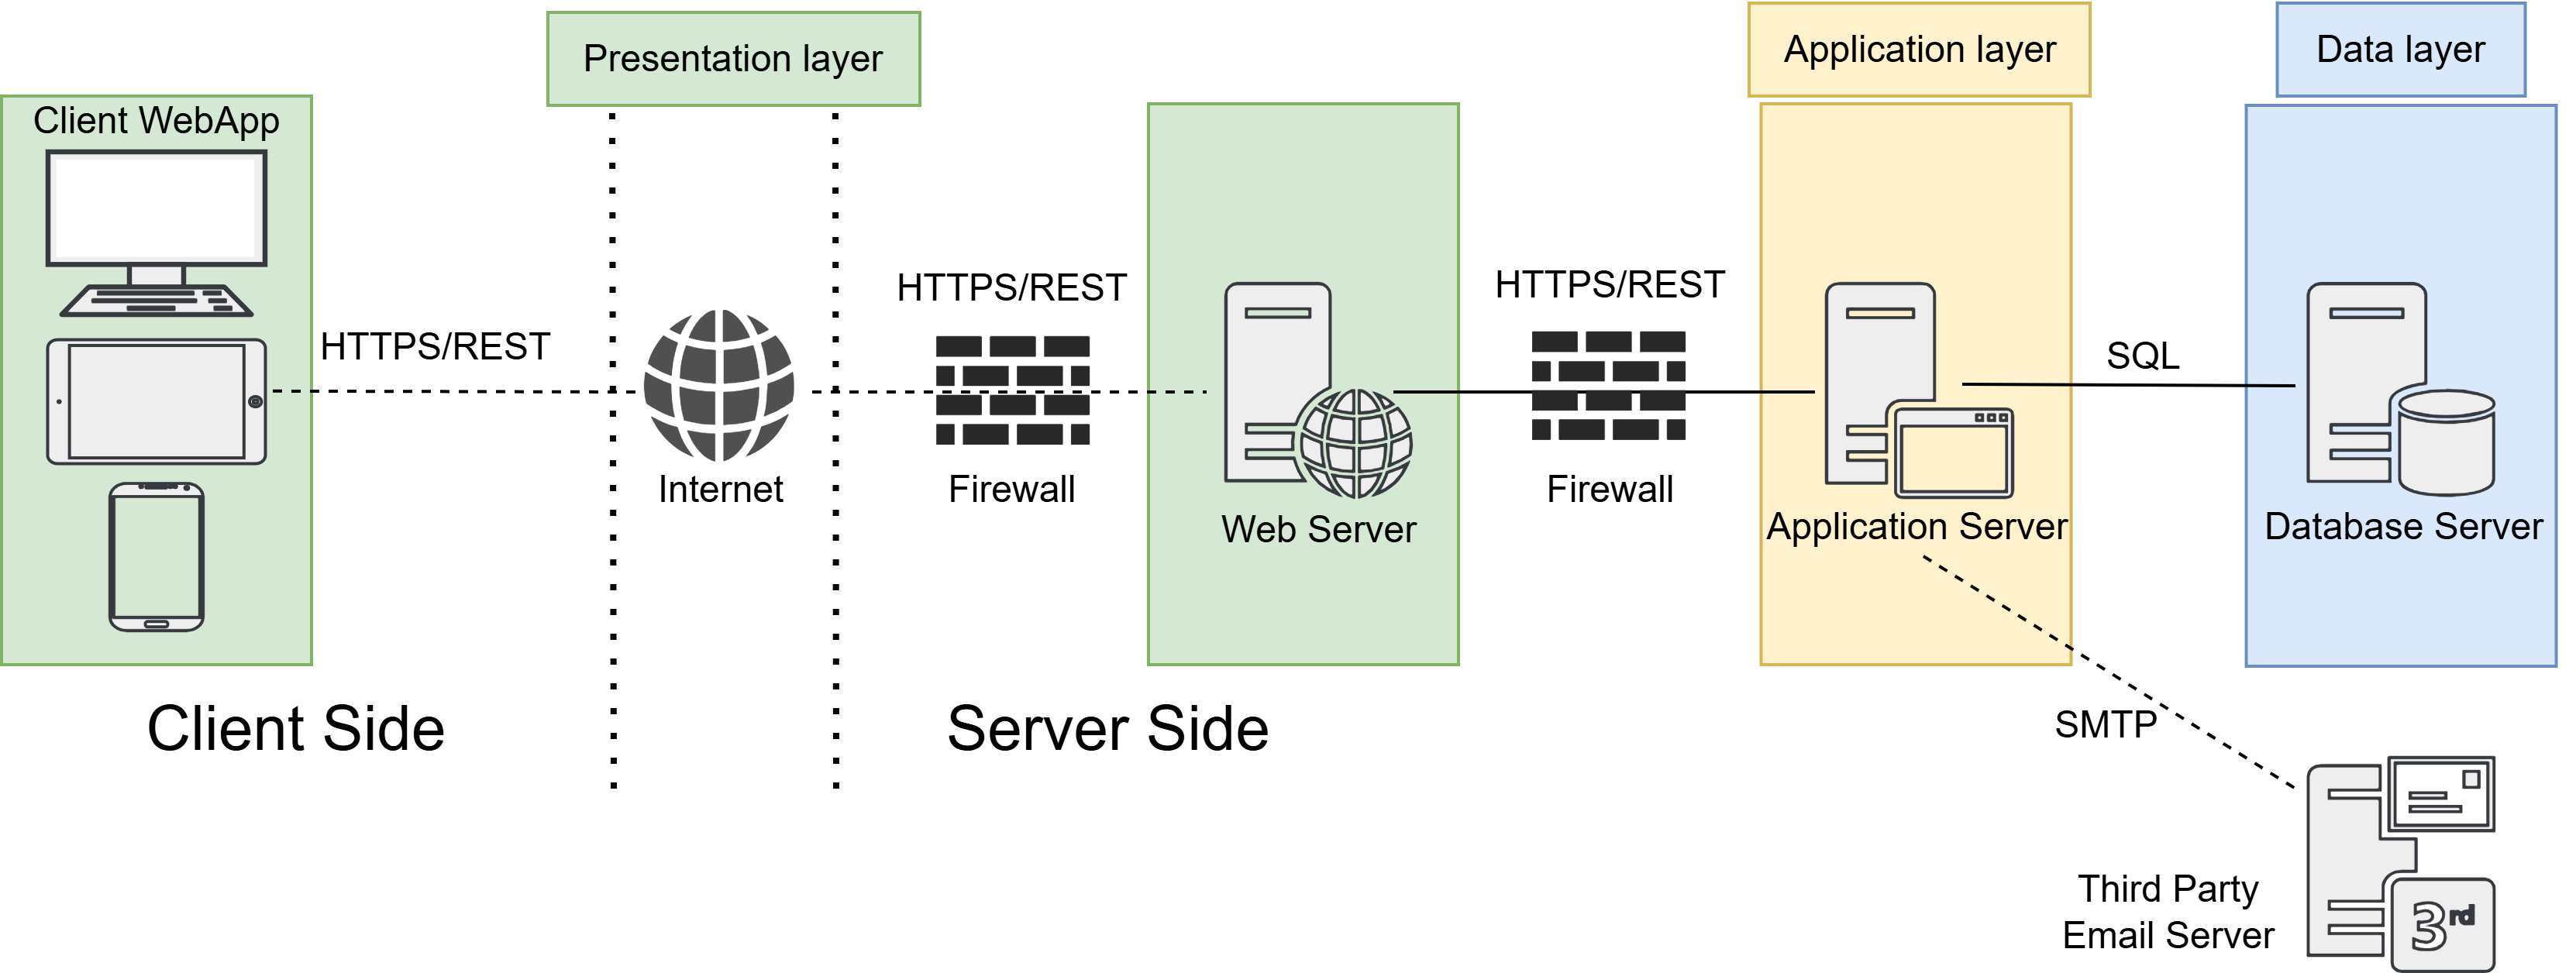
\includegraphics[width=1\textwidth]{Images/tiers_architecture.png}
    \caption{S\&C architectural overview}\label{fig:tiers_architecture}
\end{figure}

In the following paragraph we describe each tier presented in Figure \ref{fig:tiers_architecture}: and what layer it deploys:
\paragraph{Client Side}
\begin{itemize}
    \item \textbf{Web App:} It is the user interface. It will be responsible for managing the user interaction. This means that it will be responsible 
    for hosting part of the presentation layer. 
\end{itemize}

\paragraph{Server Side}
\begin{itemize}
    \item \textbf{Firewall:} It will be responsible for managing the security of the system, by filtering the incoming and outgoing traffic and restricting
    the access based on predefined rules. It will be placed between the Web Server and the Internet and between the Application Server and the Web Server.
    In this way, the web server will reside in a DMZ (Demilitarized Zone), while the application server will reside in a protected internal network.
    \item \textbf{Web Server:} It serves as a gateway between the client and the application server (backend). It will be responsible for hosting part 
    of the presentation layer. For example, it will be responsible for serving the web pages to the client, handling requests routing to the application
    server, managing load balancing, and handling security.
    \item \textbf{Application Server:} It will be responsible for managing the application logic. This means that it will host the application layer. For 
    example, it will be responsible for processing the client requests, execute the business logic, and coordinates with the database and email server.
    \item \textbf{Database Server:} It will be responsible for managing the data storage and the data access. This means that it will host the data layer.
    For example, it will be responsible for storing and retrieving the application data, and executing the database queries.
    \item \textbf{Mail Server:} It will be responsible for managing the email communication. This means that it will be responsible for sending emails to 
    the users. It is triggered by the application server.
\end{itemize}

The Figure \ref{fig:tiers_architecture} also shows how the tiers interact with each other. The Web App interacts with the Web Server through HTTPS/REST 
requests; the Web Server interacts with the Application Server through HTTPS/REST calls; the Application Server interacts with the Database Server through 
SQL queries; and the Application Server interacts with the Mail Server through SMTP requests.



\section{Components view}\label{sec:components view}
In this section we describe the components of the S\&C platform, their interactions, and the interfaces they expose. For understandability we divide the
components into two categories: high-level components and low-level components.

\subsection{High-level components and interactions}\label{subsec:high-level components and interactions}
\begin{figure}[H]
    \centering
    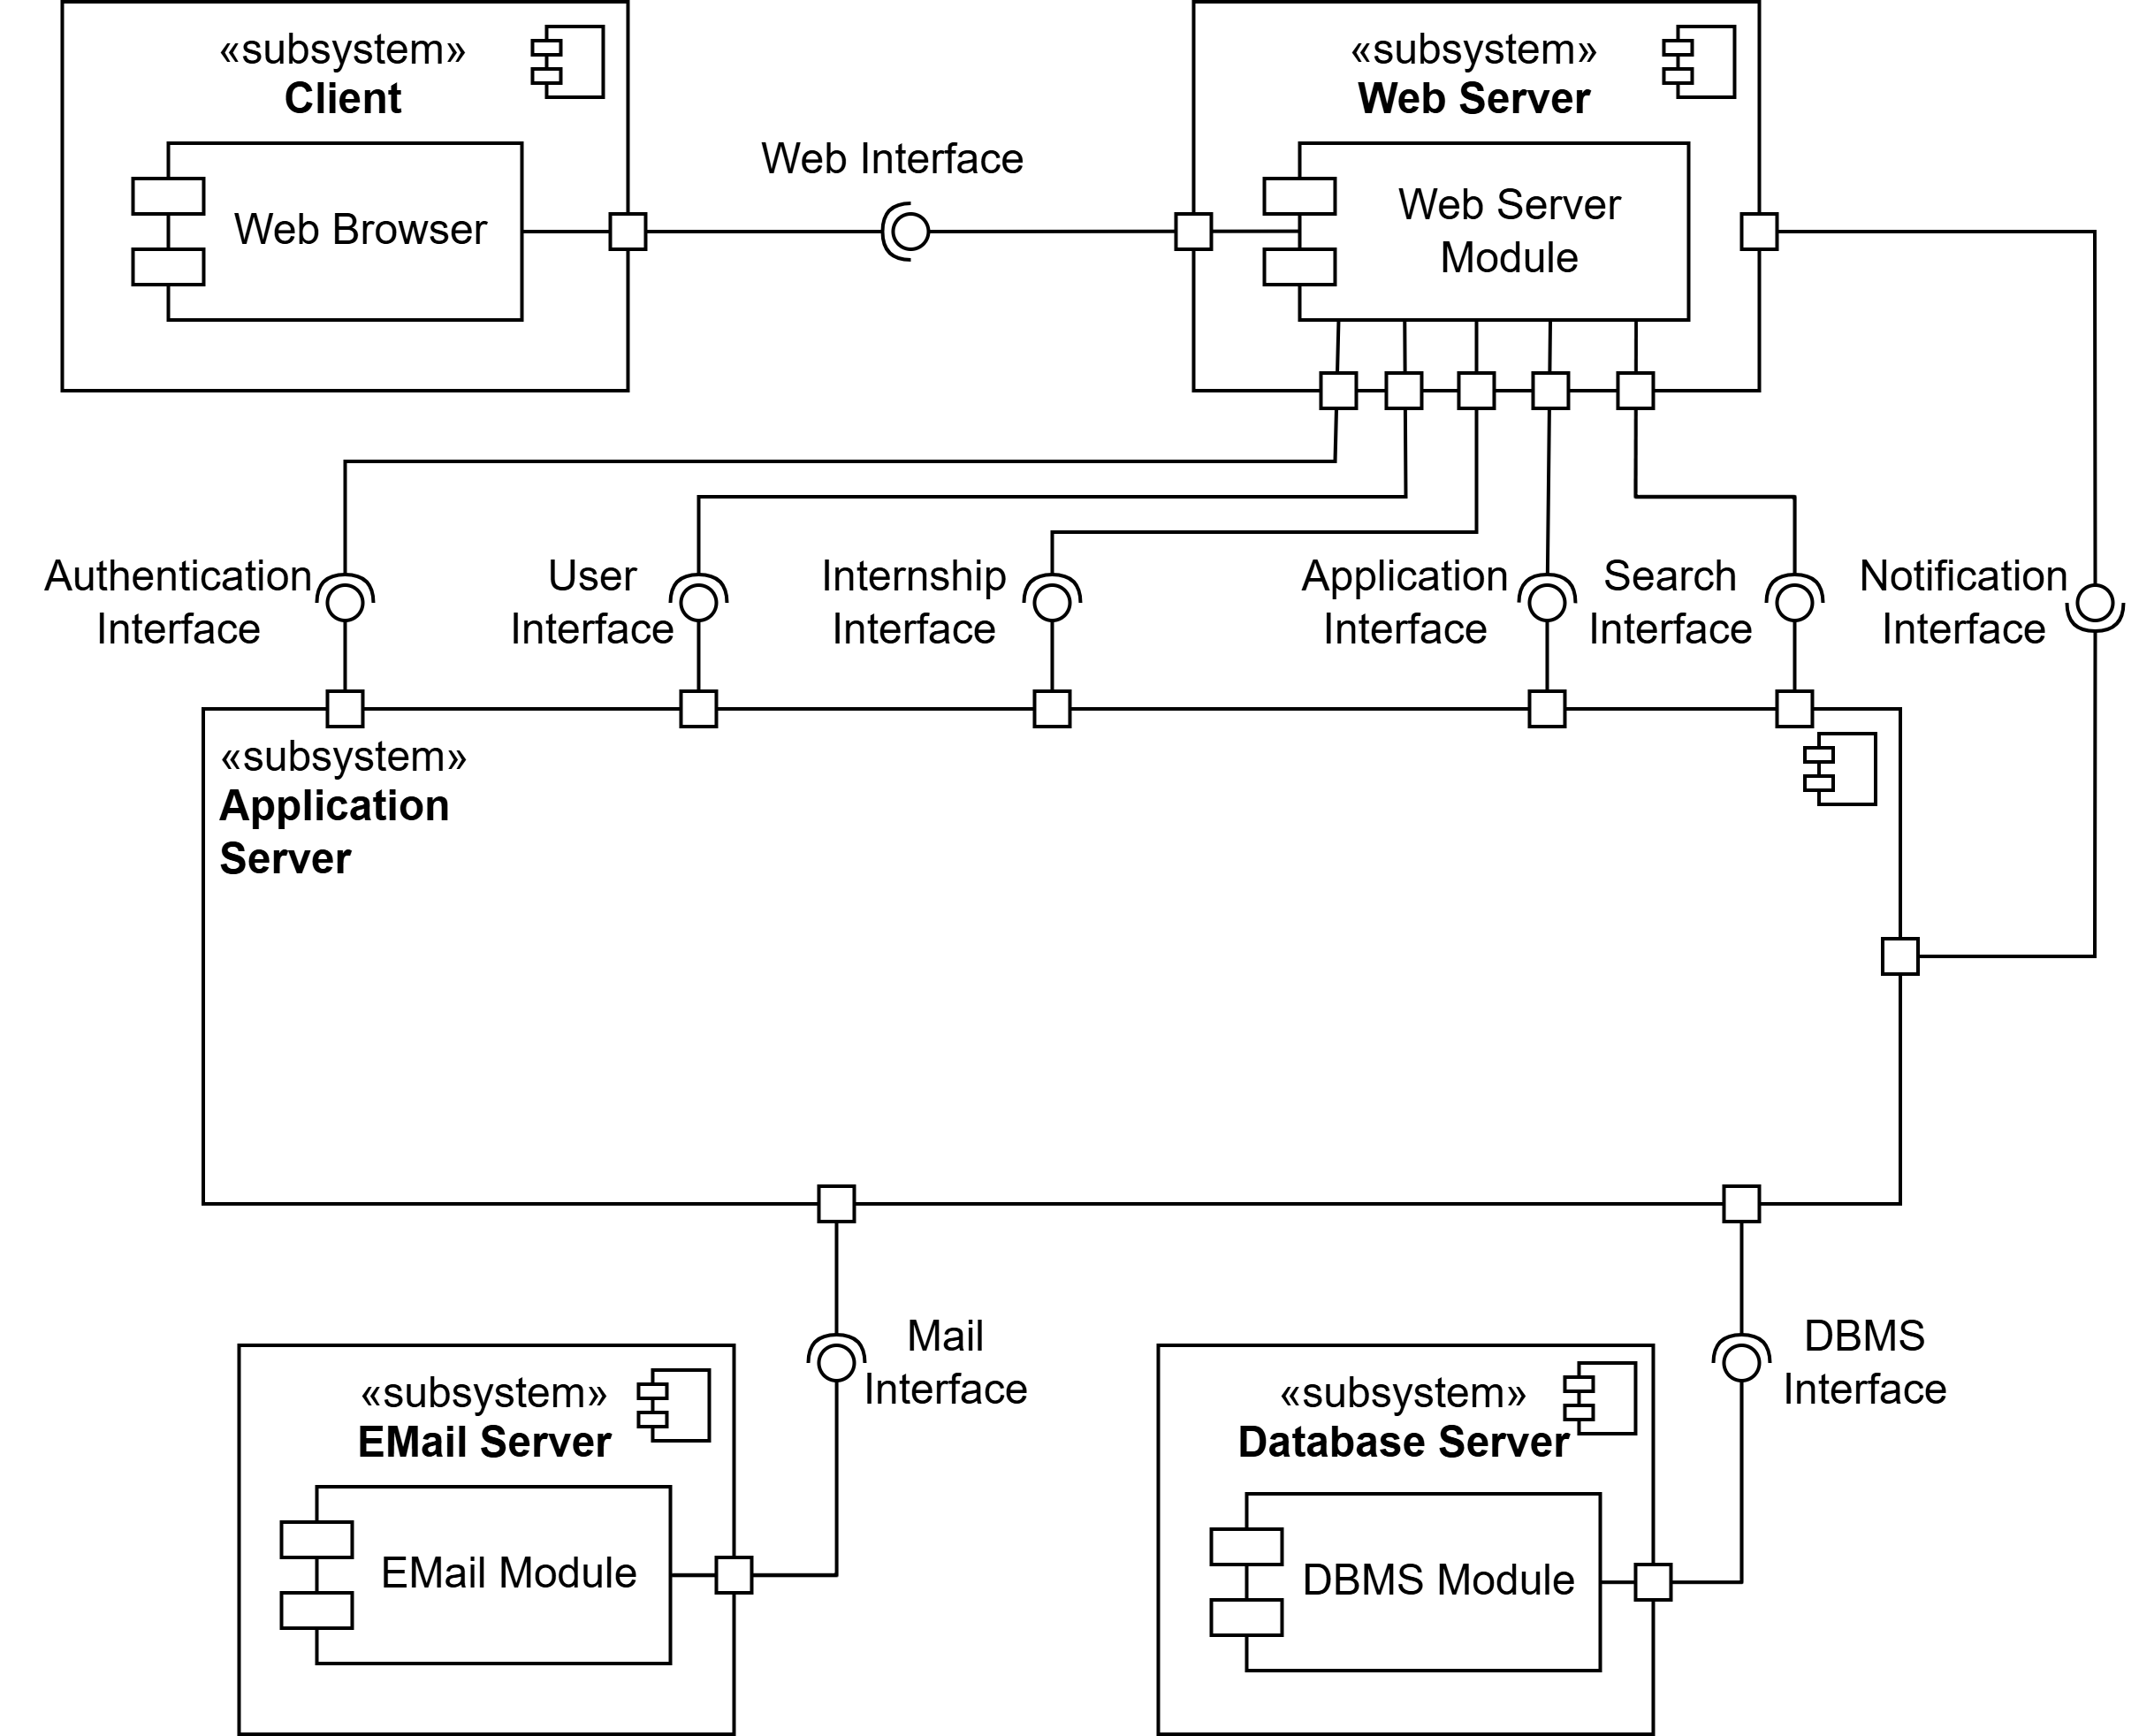
\includegraphics[width=1\textwidth]{Images/Components/HL_Component_Diagram.png}
    \caption{High Level Component Diagram}\label{fig:hl_component_diagram}
\end{figure}
In the figure above we show the high-level components of the S\&C platform. In particular we show which are the components that are run on each tier of 
the system.
\begin{itemize}
    \item \textbf{Web Browser:} It serves as the external interface for the user to interact with the platform. It sends requests to the Web Server and
    receives responses from it. It is responsible for rendering the web pages and handling user input.
    \item \textbf{Web Server Module:} It serves as a gateway between the client and the application server. It handles load balancing and security, 
    ensuring that requests are properly routed through the interfaces that are provided by the application server. It also provides the Notification 
    Interface, which allows the Web Server Module to send notifications to users.
    \item \textbf{Application Server:} Hosts all the system's internal components and provides the following interfaces: Authentication Interface, User 
    Interface, Internship Interface, Application Interface, and Search Interface. 
    \item \textbf{DBMS:} It communicates with the application server through the DBMS Interface and is responsible for managing the data storage and 
    retrieval operations. It ensures data consistency and integrity, and provides mechanisms for data backup and recovery. 
    \item \textbf{Email Server:} It is responsible for the sending of emails for user registration confirmation. The Application Server interacts with 
    the Email Server via the Email Interface to send these emails.
\end{itemize}

\subsection{Low-level components and interactions}\label{subsec:low-level components and interactions}
\begin{figure}[H]
    \centering
    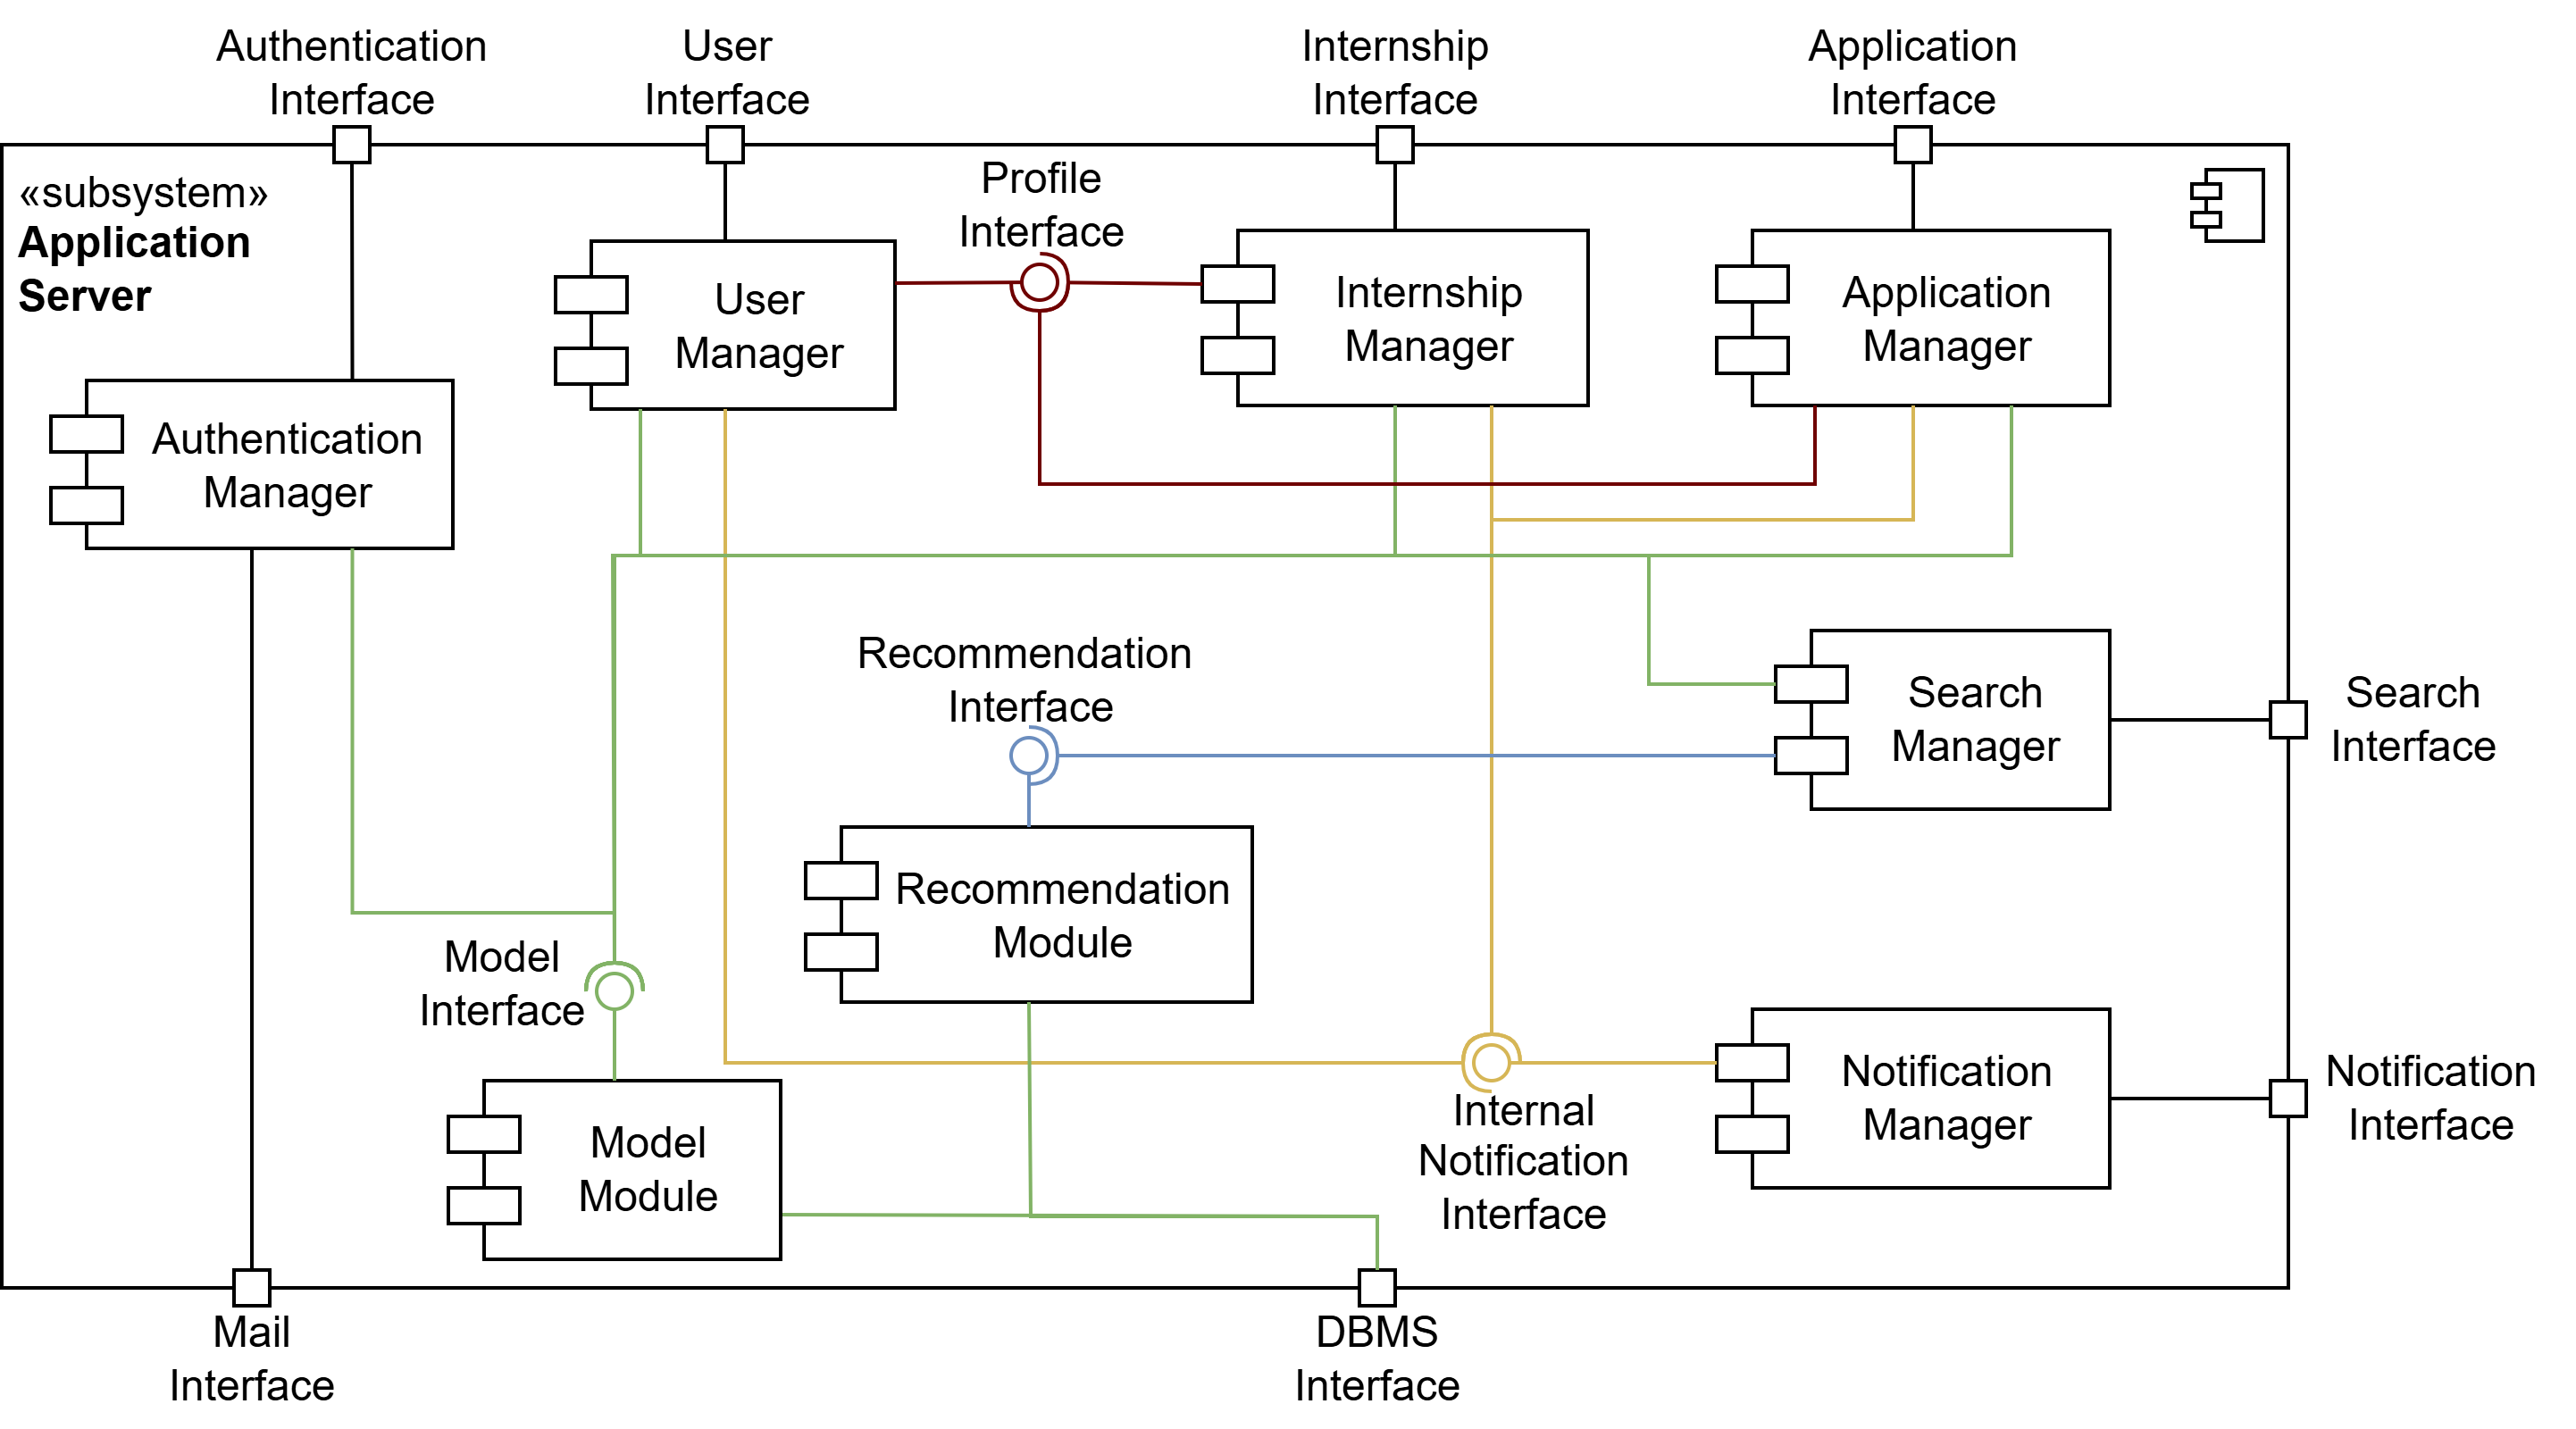
\includegraphics[width=1\textwidth]{Images/Components/LL_Component_Diagram.png}
    \caption{Low Level Component Diagram}\label{fig:ll_component_diagram}
\end{figure}
In Figure \ref{fig:ll_component_diagram}, we show the low-level components of the platform. In particular, these components provide more detailed 
insights into the internal workings of the Application Server. The low-level components are divided as follows:
\subsubsection{Authentication Manager}
This component manages user authentication and authorization processes. It interacts with the Model Module through the provided
interface in order to store and retrieve information from the database. It includes the following subcomponents:
\begin{itemize}
    \item \textbf{Registration Manager:} It is responsible for managing the user registration process, including the creation of new user accounts 
    and sending verification emails through the Mail Interface.
    \item \textbf{Login Manager:} It is responsible for managing the user login process, including verifying user credentials and maintaining user sessions.
\end{itemize}
\begin{figure}[H]
    \centering
    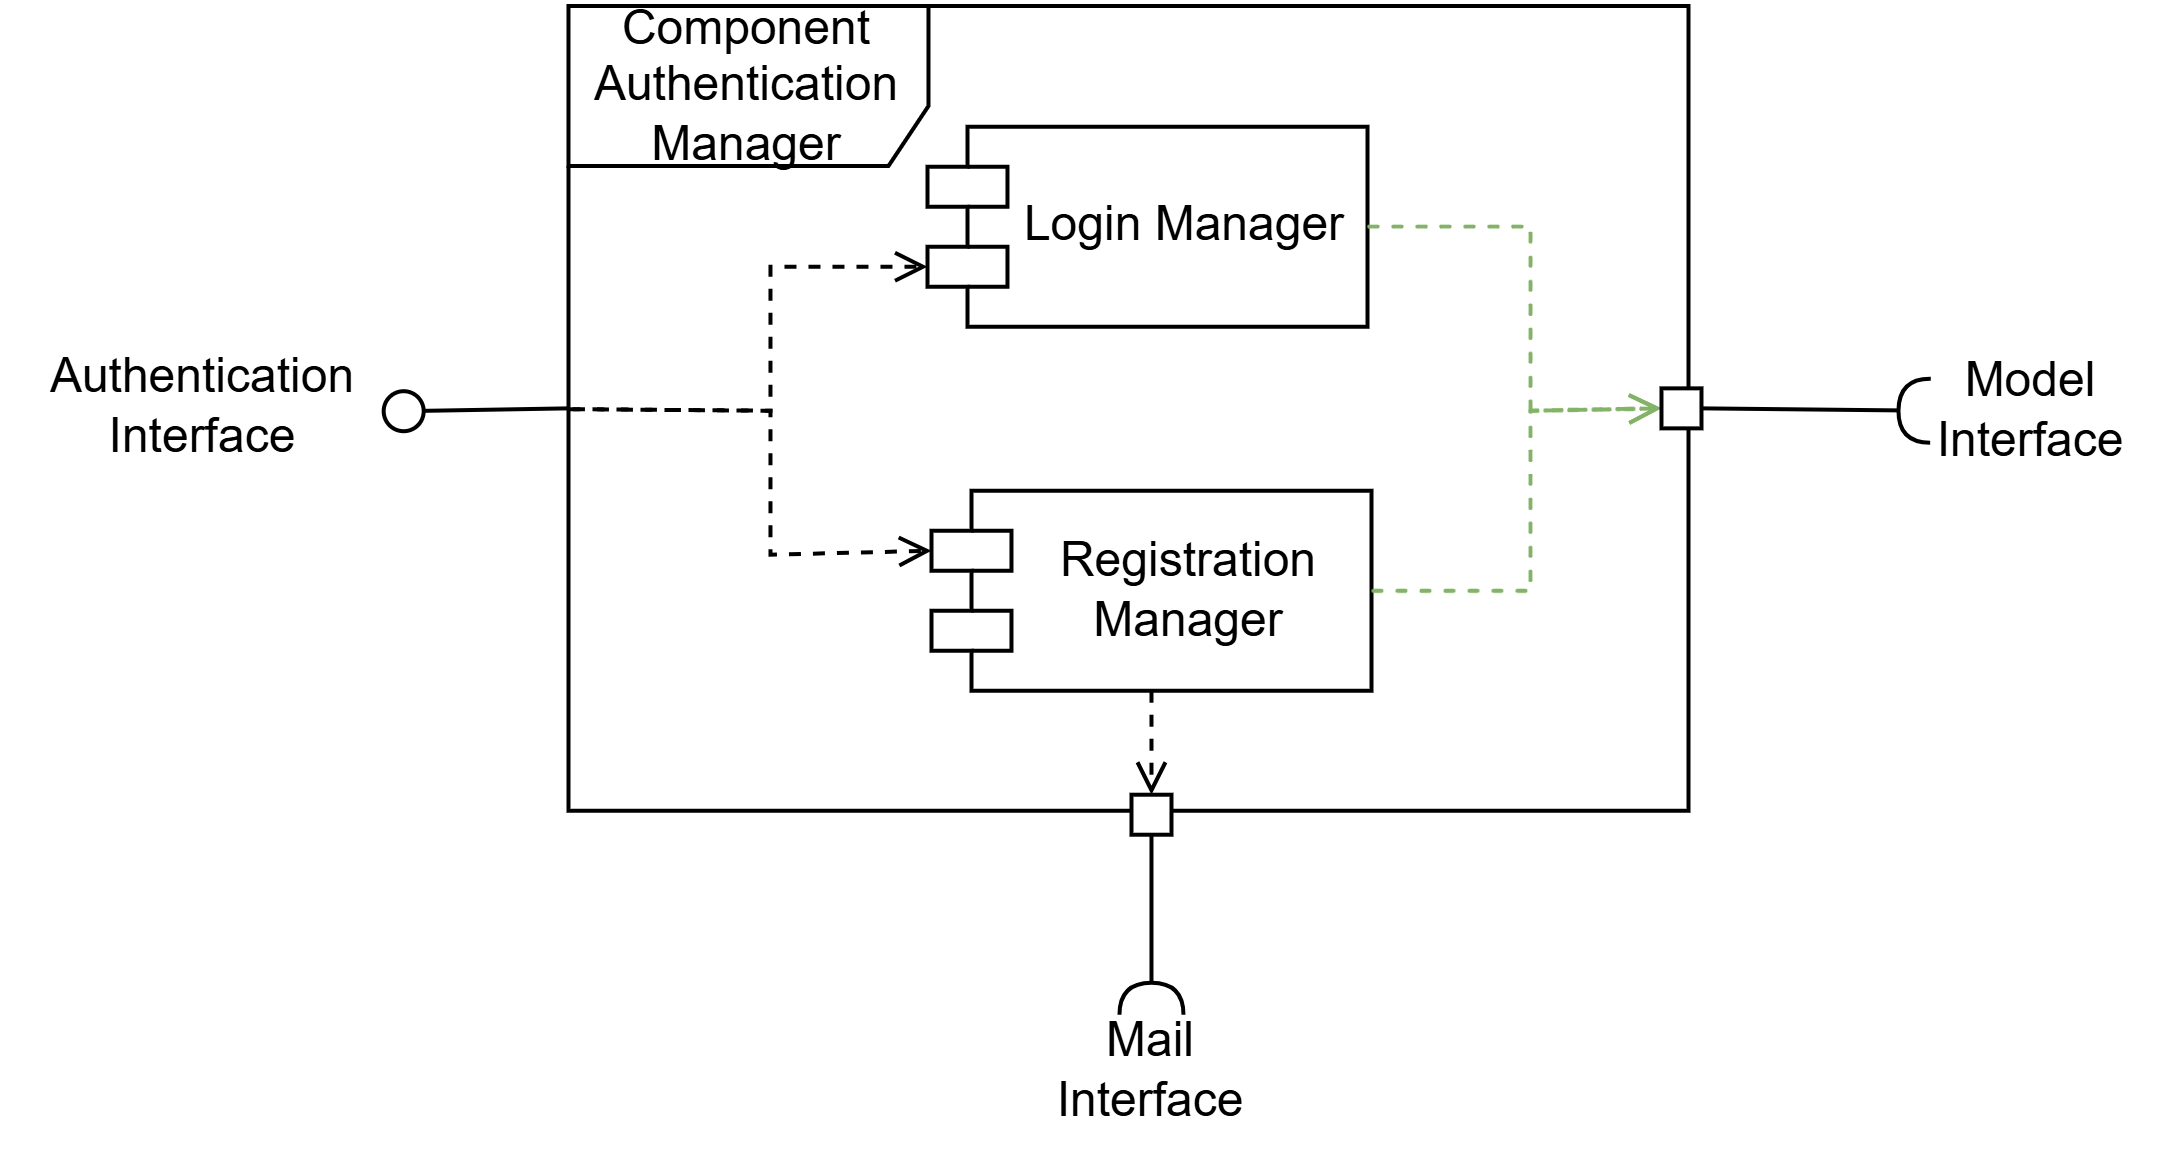
\includegraphics[width=0.75\textwidth]{Images/Components/auth_Component.png}
    \caption{Authentication Manager}\label{fig:auth_manager}
\end{figure}
\subsubsection{User Manager}
This component is responsible for managing user-related operations, such as user profile management and visualization, and handling user-specific 
notifications. It interacts with the Model Module to store and retrieve user information from the database.
\begin{itemize}
    \item \textbf{View Profile Manager:} Provides users with an overview of their activities and notifications. It provides a Profile Interface that
    allows other components to access user data.
    \item \textbf{Profile Modification Manager:} Allows users to view and edit their personal information.
\end{itemize}
\begin{figure}[H]
    \centering
    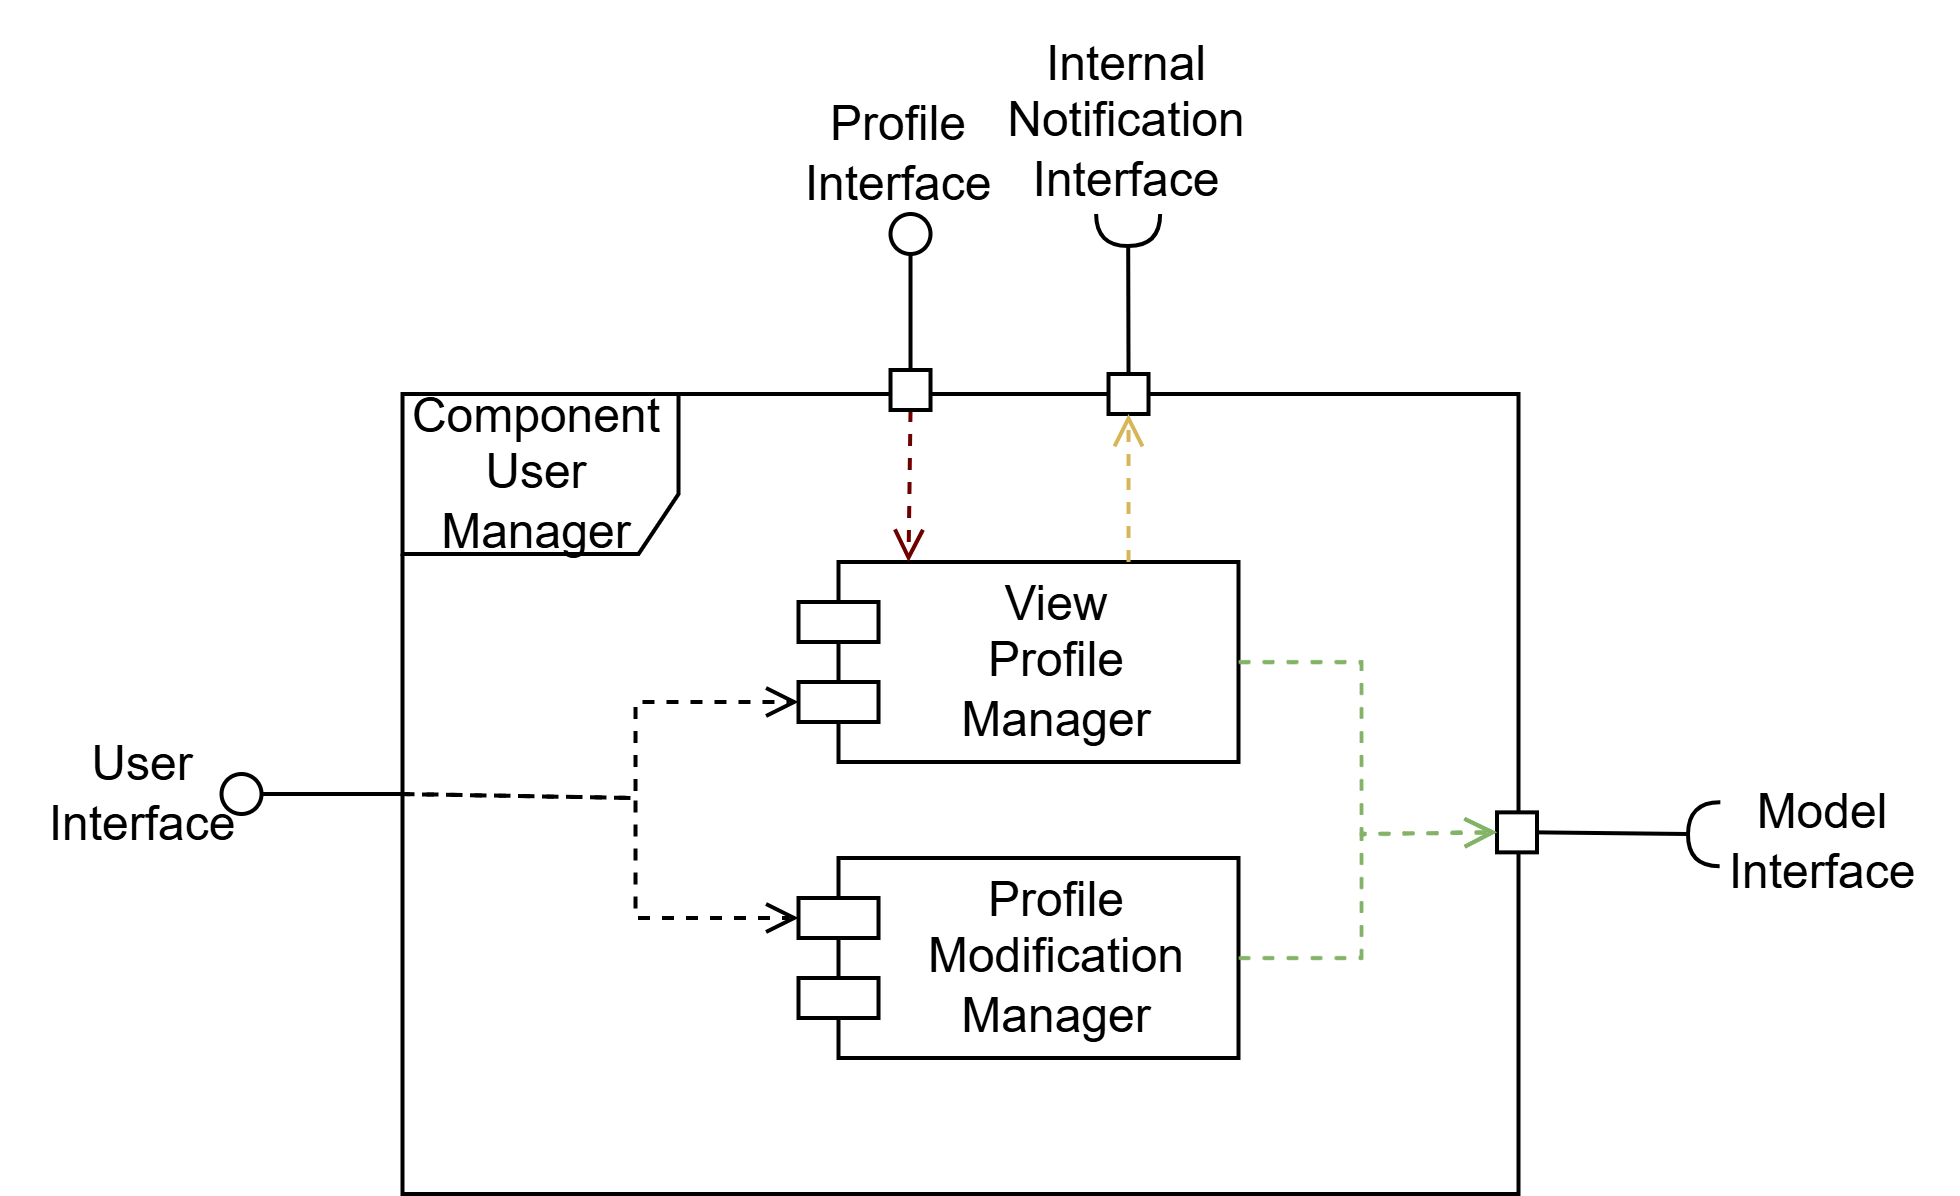
\includegraphics[width=0.75\textwidth]{Images/Components/user_Component.png}
    \caption{User Manager}\label{fig:user_manager}
\end{figure}
\subsubsection{Internship Manager}
The Internship Manager is the component used by the S\&C platform to manage internship-related operations. It interacts with the Model Module to store
and retrieve internship information and related data (such as chat messages and feedback) from the database. It includes the following subcomponents:
\begin{itemize}
    \item \textbf{Creation Manager:} Manages the creation of internship and their posting. 
    \item \textbf{View Internship Information Manager:} Manages the display of internship information when users request them.
    \item \textbf{Selection Manager:} Manages the selection process for internships. It allows companies to go through the list of applications and select 
    candidates for their internships. After the interview phase, it also allows them to decide whether to accept or reject a candidate for the internship. 
    It interacts with the Internal Notification Interface to notify students in case they are selected for interviews and in case they are accepted or rejected 
    for an internship.
    \item \textbf{Chat Manager:} Manages the chat functionality between student and company. It interacts with the Notification Manager through the provided
    interface to notify users when they receive a new message.
    \item \textbf{Feedback Manager:} Manages the feedback system for internships, allowing both companies and students to provide feedback on their internship 
    experience. It interacts with the Notification Manager through the provided interface to notify users when they receive new feedback.
\end{itemize}
The View Internship Information Manager, Chat Manager, and Feedback Manager also interact with the View Profile Manager through the provided Profile Interface,
since they need to show to both students and companies other users profile information.
\begin{figure}[H]
    \centering
    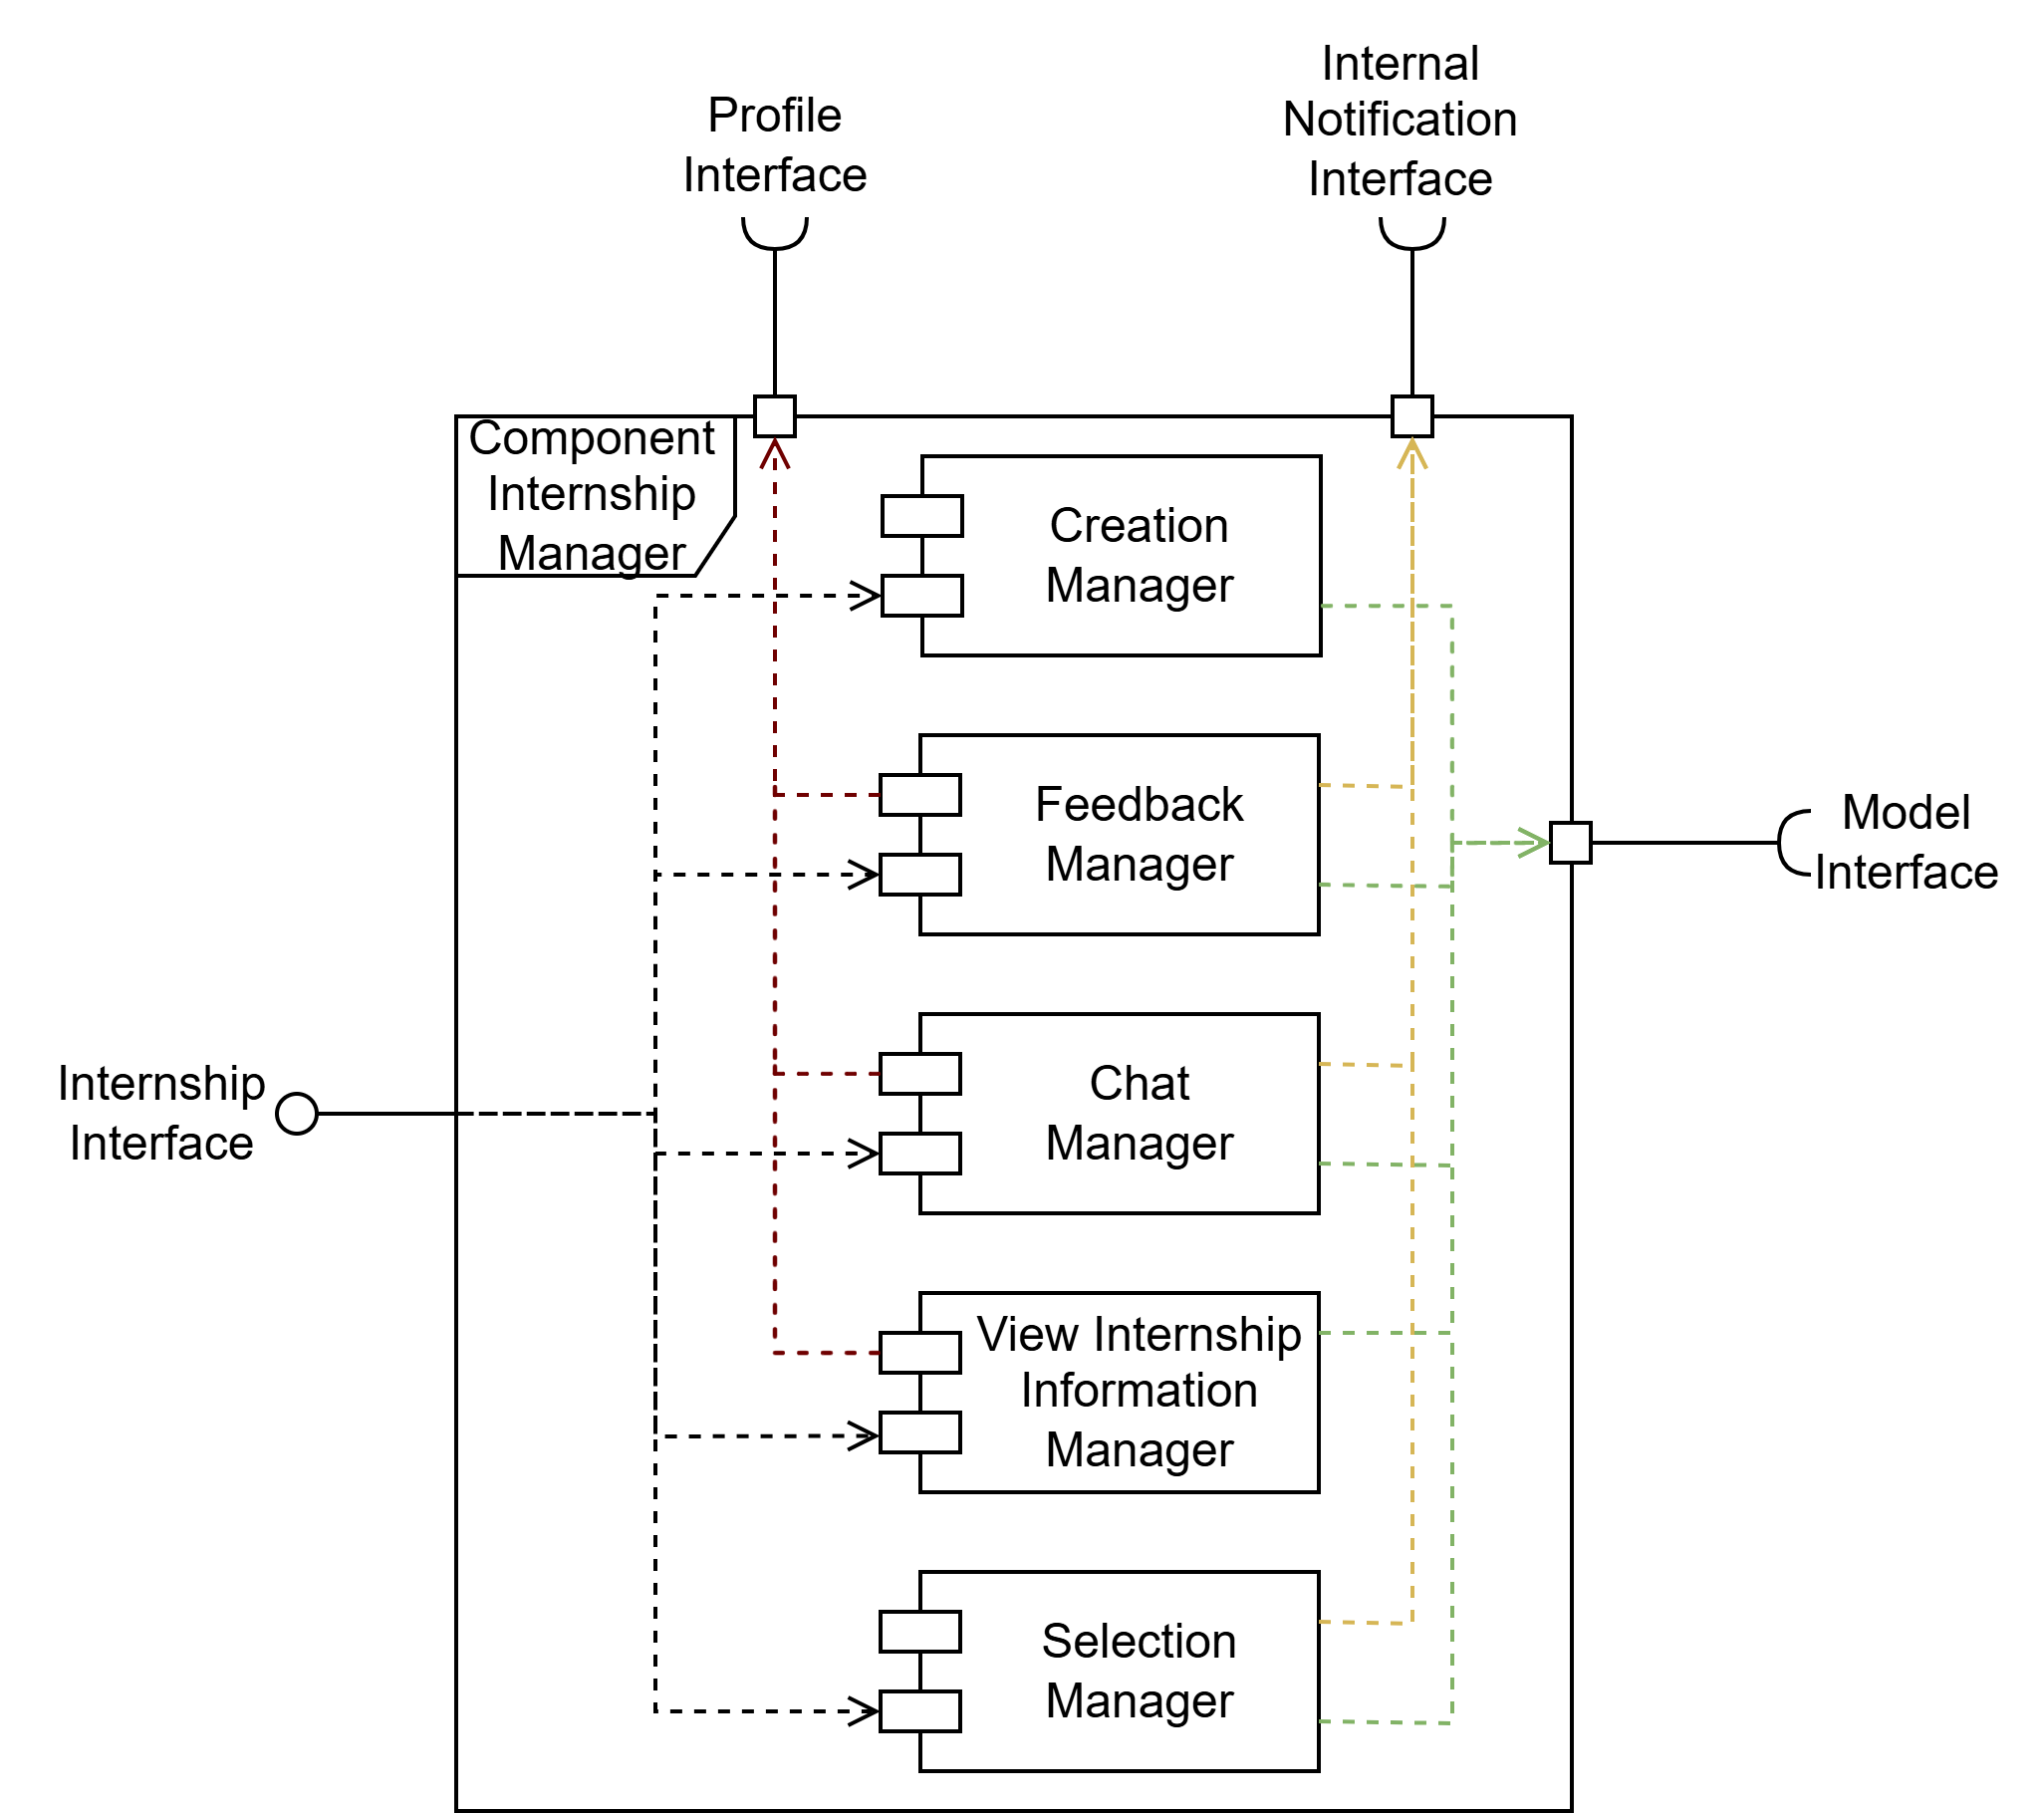
\includegraphics[width=0.75\textwidth]{Images/Components/internship_Component.png}
    \caption{Internship Manager}\label{fig:internship_manager}
\end{figure}
\subsubsection{Application Manager}
The Application Manager is the component used by the S\&C platform to handle every aspect of the application process for internships. It interacts with the
Model Module to store and retrieve application information and related data from the database. It includes the following subcomponents:
\begin{itemize}
    \item \textbf{Submission Manager:} Handles the submission of applications for internships. It allows students to apply for internships and submit their
    applications. It also allows candidates who have been accepted for the internship to accept or reject the offer from the company. It interacts with the 
    Internal Notification Interface to notify students when their application status changes.
    \item \textbf{View Application Information Manager:} Manages the display of application information to users who request them and have the rights to access
    them.
    \item \textbf{Interview Manager:} Manages the interview process for applications; it allows companies to create and modify interview forms and record 
    the results of interviews. It interacts with the Internal Notification Interface to notify students when they are selected for interviews, and notify 
    companies when the results of the interviews are available. 
    \item \textbf{Questionnaire Manager:} Manages the questionnaire system for applications, allowing students to respond to interview questions and both 
    students and companies to view the responses. It interacts with the Internal Notification Interface to notify companies when a student has completed the 
    interview form.
\end{itemize}
The View Application Information Manager, Interview Manager, and Submission Manager also interact with the View Profile Manager through the provided Profile
Interface, since they need to show to both students and companies other users profile information.
\begin{figure}[H]
    \centering
    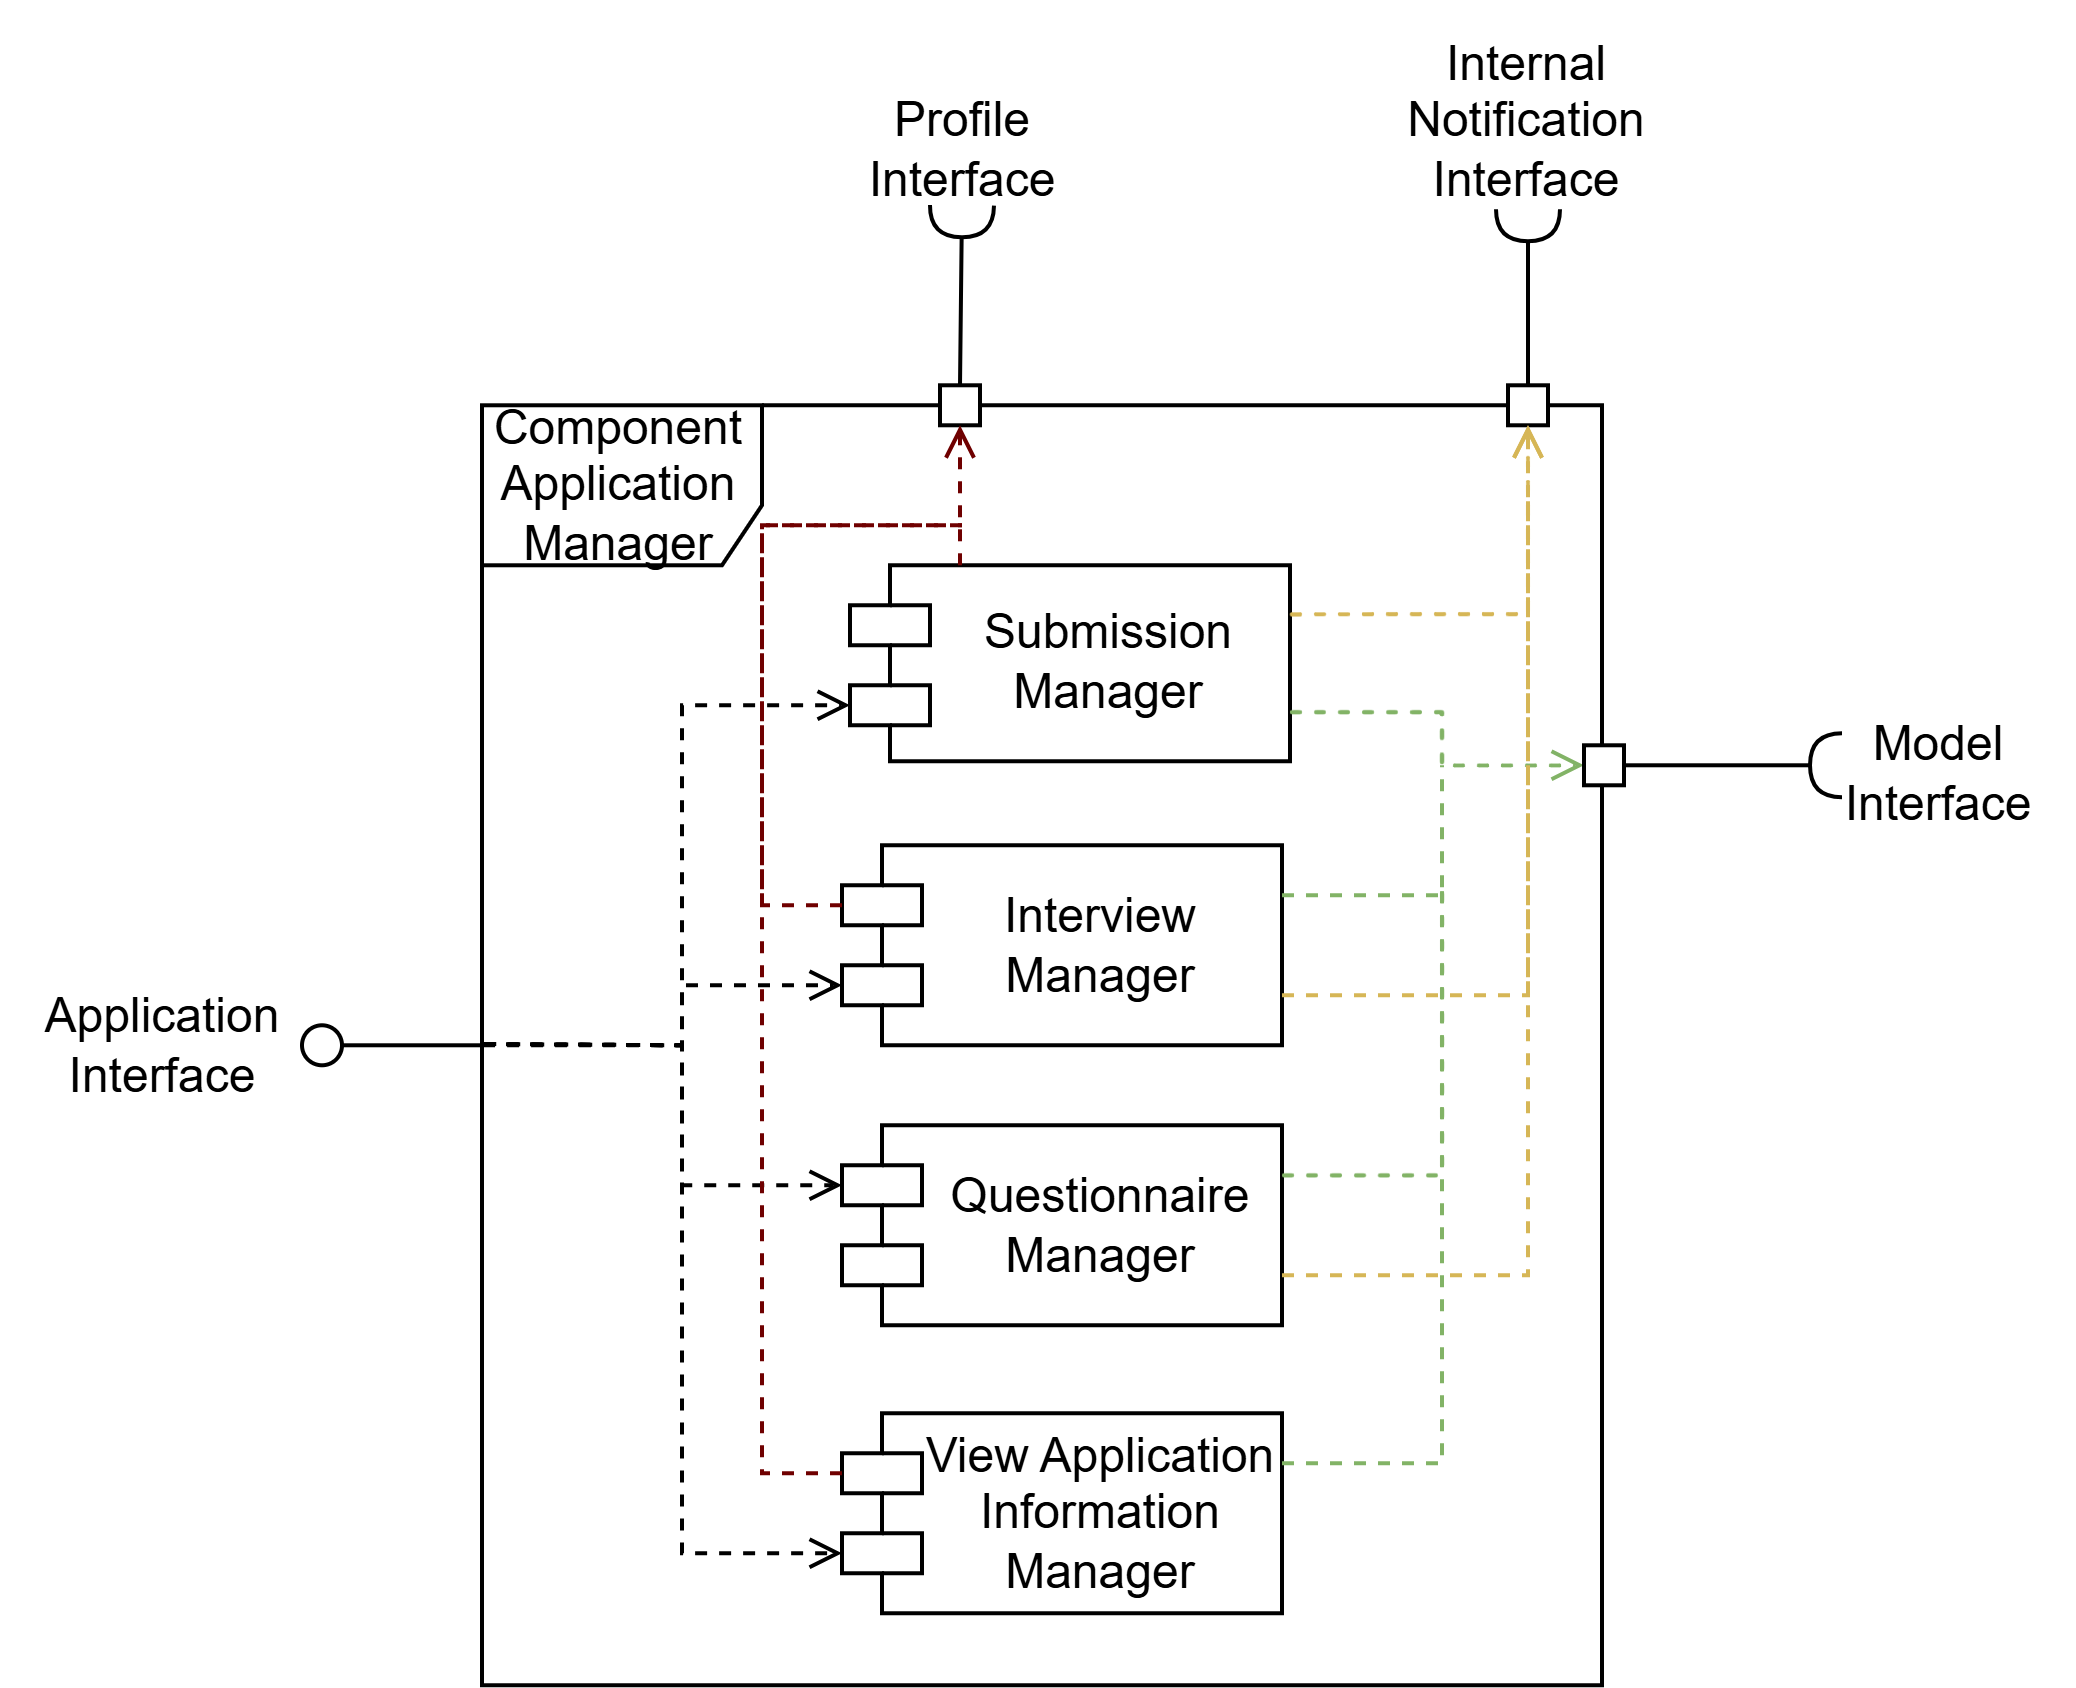
\includegraphics[width=0.75\textwidth]{Images/Components/application_Component.png}
    \caption{Application Manager}\label{fig:application_manager}
\end{figure}
\subsubsection{Search Manager}
The Search Manager is responsible for managing the search functionality of the platform, allowing users to search using filters or keywords. It interacts with 
the Model Module to retrieve search results from the database. It also interacts with the Recommendation Module to provide personalized, real-time 
recommendations to users.
\subsubsection{Notification Manager}
The Notification Manager is responsible for managing the notification system of the platform, allowing users to receive real-time updates on their activities.
It provides an Internal Notification Interface that allows other components to send notifications to users.
\subsubsection{Recommentation Module}
The Recommendation Module is responsible for generating personalized recommendations for users based on their interests, skills, and activities. It interacts
directly with the DBMS Server to retrieve the necessary information from the database in order to provide recommendations to users. It also interacts with the 
Search Manager to provide real-time recommendations based on search results.
\subsubsection{Model Module}
The Model Module is responsible for managing the data storage and retrieval operations of the platform. It interacts with the DBMS to store and retrieve
information from the database. It provides the Module Interface that allows other components to access the data stored in the database.



\section{Deployment view}\label{sec:deployment view}
\begin{figure}[H]
    \centering
    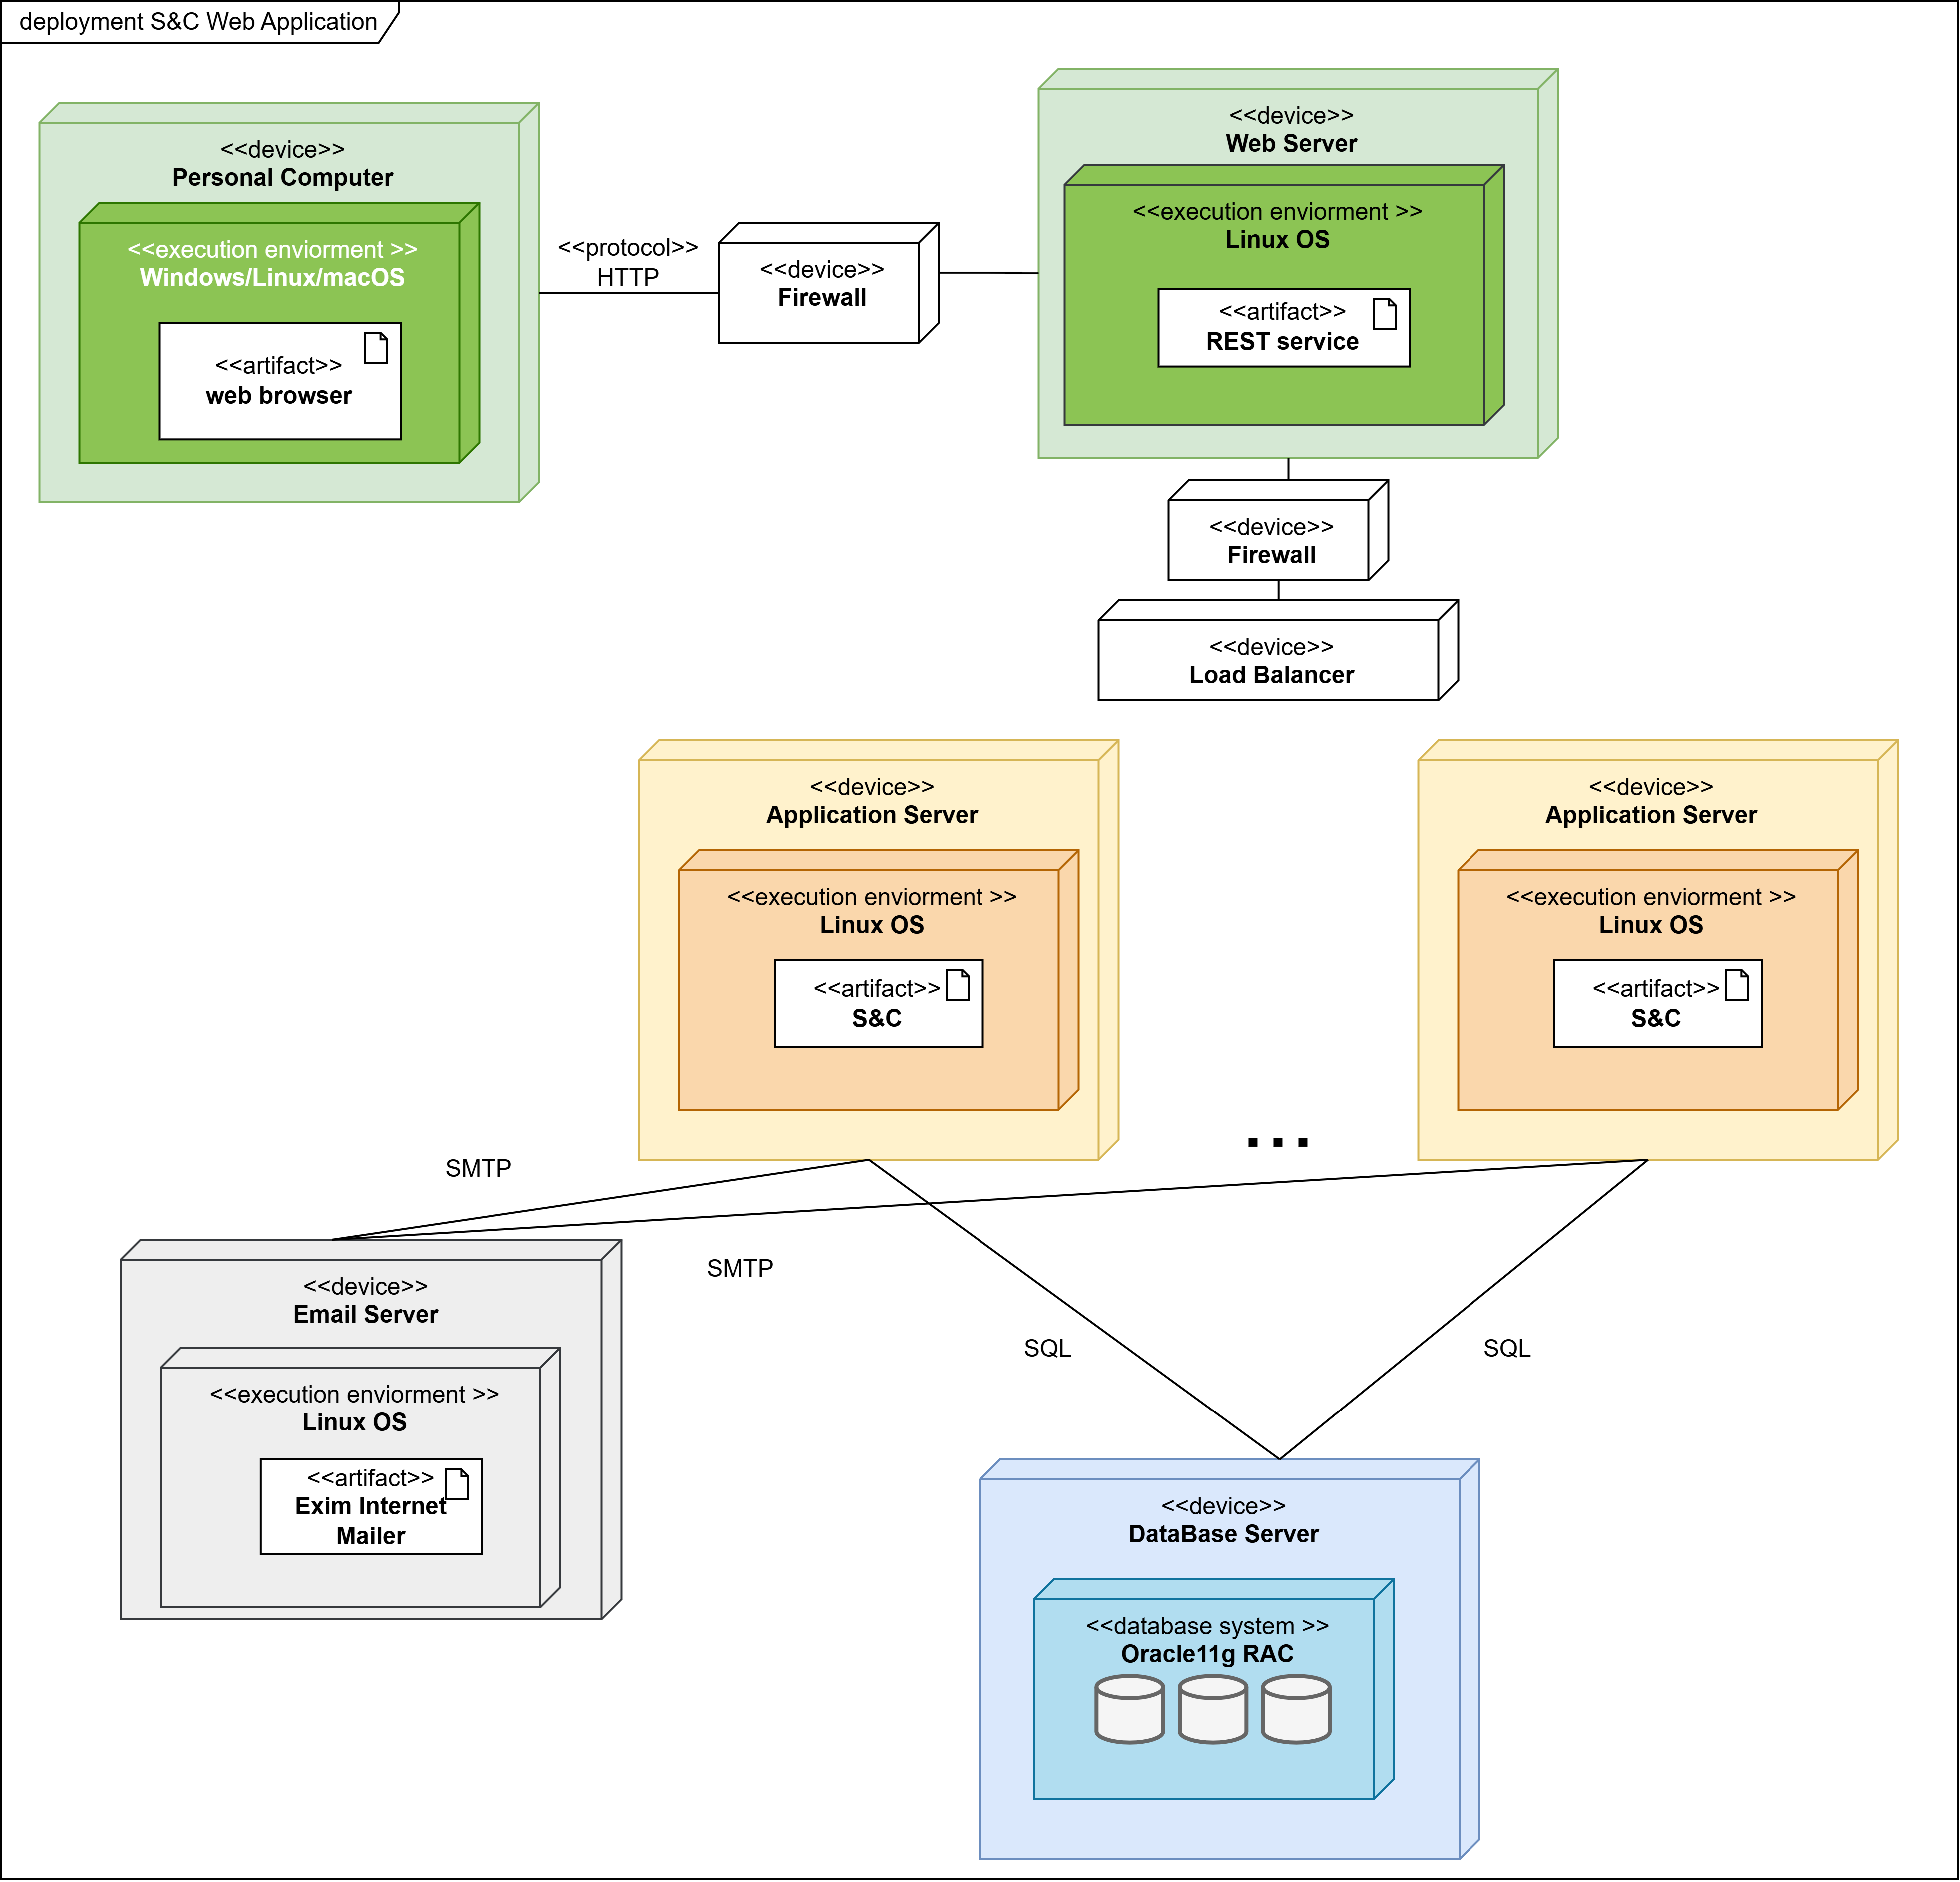
\includegraphics[width=1\textwidth]{Images/Deployment_View.png}
    \caption{S\&C deployment diagram}\label{fig:deployment_diagram}
\end{figure}
The infrastructure of the S\&C platform is described in below using a deployment diagram and a description of the components and their interactions.
As described at the beginning of this document, the system is divided into three layers: the presentation layer, the application layer, and the data layer.
The deployment diagram in Figure \ref{fig:deployment_diagram} shows the physical distribution of the components across different servers and the communication
between them.

\begin{itemize}
    \item \textbf{Personal Computer:} Anyone interested in using the platform can access it through any type of personal computer. Users can also access the 
    platform using any device capable of running a web browser. This component communicates and interacts with the Web Server via HTTPS protocols and RESTful 
    API services.
    \item \textbf{Web Server:} The Web Server hosts the web application and serves web pages to users. It handles HTTP requests from clients and forwards them 
    to the Application Server. Together with the Firewall and Load Balancer, it ensures the security, scalability, and availability of the system. It acts as 
    a gateway between the client and the Application Server.
    \item \textbf{Application Server:} This component contains the core application logic of the platform, managing the operations necessary to provide services 
    and functionalities to users. Thanks to RESTful API services and the Load Balancer, it can handle multiple requests simultaneously without the risk of 
    overloading or crashing. It interacts with the Database Server to access or store data, such as recording a student's new internship. Additionally, it 
    communicates with the Mail Server, particularly during user registration, to authenticate email addresses and verify user identities.
    \item \textbf{Database Server:} Most primary operations of the platform require frequent interaction with the Database Server. This component manages 
    personal data, tracks the progress of applications and internships, stores chat histories between users, and more. The Application Server retrieves or 
    stores data using SQL queries.
    \item \textbf{Mail Server:} During the registration process, the platform requires users to verify their email addresses to confirm their identity and 
    complete account creation. The Application Server interacts with the Mail Server via SMTP requests to send verification emails.
    \item \textbf{Firewall:} The Firewall protects the core components of the system by filtering incoming and outgoing traffic and restricting access based on 
    predefined rules. For example, if an unauthorized individual attempts to access the Application Server and modify data in the Database Server without proper 
    credentials, the Firewall blocks the attempt, preventing unauthorized access.
    \item \textbf{Load Balancer:} The Load Balancer distributes incoming client requests to ensure that no one application server is overwhelmed to operate at 
    peak efficiency. It is placed between the Web Server and the Application Server, in order to optimize the performance and availability of the system.
\end{itemize}

\section{Component interfaces}\label{sec:component interfaces}
In the following paragraphs, we describe the interfaces of the main components of the platform specifying the methods that each component can perform.
Note: 

- \textit{userId} are unique identifiers generated by the system for each user once they register on the platform and are used to access the data related to 
that user.

- \textit{userTypes} enumeration is used to distinguish between the different types of users that can register on the platform: Student, Company, University.

- \textit{SearchType} enumeration used to distinguish between the different types of searches that can be performed on the platform: Internship and User Profile.

- \textit{NotificationType} enumeration used to distinguish between the different types of notifications that can be sent on the platform in order to handle 
them in a different way.

- \textit{InternshipID} is a unique identifier generated by the system for each internship published successfully and is used to access the data related to 
that internship.

- \textit{ChatID} is a unique identifier generated by the system for each chat created between two users and is helpful to access the data related to that 
chat more easily.

- \textit{ApplicationID} is a unique identifier generated by the system for each application submitted by a student for an internship and is used to access 
the data related to that application and take a track of its status.


\subsubsection{authorization Manager}
\paragraph{Registration Manager}
\begin{itemize}
    \item[-] registration (String email, String password, String name, String surname, University university, List[Field] interests, List[String] skills): Boolean
    \item[-] registration (String email, String password, String legalName, String EIN, String department, List[Field] fields): Boolean
    \item[-] registration (String email, String password, String name, String legalName): Boolean
    \item[-] generateUserId (): int
    \item[-] confirmRegistration (String email): Boolean 
\end{itemize}

\paragraph{Login Manager}
\begin{itemize}
    \item[-] login (String email, String password): Boolean
\end{itemize}


\subsubsection{User Manager}
\paragraph{Profile Modification Manager}
\begin{itemize}
    \item[-] uploadCV (int userId, File cv): Boolean
    \item[-] updatePersonalInfo (int userId, String name, String surname): Boolean
    \item[-] updateUniversityInfo (int userId, University university): Boolean
    \item[-] updateInterestsAndSkills (int userId, List<Field> interests, List<String> skills): Boolean
    \item[-] updatePassword (int userId, String oldPassword, String newPassword): Boolean
    \item[-] updateLegalInfo (int userId, String legalName, String EIN, String department): Boolean
    \item[-] updateProfilePicture (int userId, File profilePicture): Boolean
    \item[-] addFieldOfInterest (int userId, Field field): Boolean
    \item[-] removeFieldOfInterest (int userId, Field field): Boolean
    \item[-] addSkill (int userId, String skill): Boolean
    \item[-] removeSkill (int userId, String skill): Boolean
    \item[-] checkFileFormat (File file): Boolean
    \item[-] saveModifications (int userId): Boolean 
    \item[-] saveModifications (int userId, String email, String password, String name, String surname, University university, List[Field] interests, List[String] skills): Boolean
    \item[-] saveModifications (int userId, String email, String password, String legalName, String EIN, String department, List[Field] fields): Boolean
    \item[-] saveModifications (int userId, String email, String password, String legalName): Boolean  
\end{itemize}

\paragraph{View Profile Manager}
\begin{itemize}
    \item[-] getProfile (int userId): Profile
    \item[-] getListOfEnrolledStudents (University university): List[Student]
\end{itemize}


\subsubsection{Search Manager}
\begin{itemize}
    \item[-] search (int userId, String keyword): List[Result] and List[Recommendation]
    \item[-] searchFilterByType (int userId, SearchType type, List[Result]): List[Result]
    \item[-] searchFilterByField (int userId, Field field, List[Result]): List[Result]
    \item[-] searchFilterByLocation (int userId, String location, List[Result]): List[Result]
    \item[-] searchFilterByTime (int userId, Date startDate, Date endDate, List[Result]): List[Result]
\end{itemize}


\subsubsection{Notification Manager}
\begin{itemize}
    \item[-] notify (int userId, String notification, NotificationType type): Boolean 
    \item[-] notify (int userId, String notification): Boolean 
    \item[-] notify (String internshipId, String notification): Boolean
    \item[-] getNotifications (int userId): List[Notification]
    \item[-] getNotificationDetails (int userId): Notification
    \item[-] isRead (int userId, String notification): Boolean
    \item[-] deleteNotification (int userId, String notification): Boolean
    \item[-] deleteAllNotifications (int userId): Boolean
\end{itemize}


\subsubsection{Recommendation Module}
\begin{itemize}
    \item[-] getRecommendations (int userId): List[Recommendation]
    \item[-] generateRecommendations (int userId): List[Recommendation]
    \item[-] revaluateRecommendationsList (int userId, List[Recommendation] 
    oldRecommendations): List[Recommendation]
    \item[-] needRecommendationUpdate (int userId): Boolean
\end{itemize}


\subsubsection{Internship Manager}
\paragraph{Creation Manager}
\begin{itemize}
    \item[-] createInternship (String title, String description, Field field, String location, Date startDate, Date endDate, int duration, String position, Date deadline): Boolean
    \item[-] generateInternshipID (): String
    \item[-] addInternshipInList (String internshipId, Company company): Boolean
\end{itemize}

\paragraph{View Internship Information Manager}
\begin{itemize}
    \item[-] getInternshipInformation (String internshipId): Internship
    \item[-] getInternshipList (Company company): List[Internship]
    \item[-] getInternshipList (Student student): List[Internship]
\end{itemize}

\paragraph{Selection Manager}
\begin{itemize}
    \item[-] selectStudentForInterview (String internshipId, List[Student]): Boolean
    \item[-] selectStudentForInternship (String internshipId, List[Student]): Boolean
    \item[-] getSelectedStudents (String internshipId): List[Student]
    \item[-] updateStudentStatus (String internshipId, Student student, Status status): Boolean
    \item[-] getCandidatesList (String internshipId): List[Student]
    \item[-] acceptOffer (String internshipId, int userId): Boolean
    \item[-] rejectOffer (String internshipId, int userId): Boolean  
\end{itemize}

\paragraph{Feedback Manager}
\begin{itemize}
    \item[-] writeFeedback (int userId, String internshipId, String feedback): Boolean
    \item[-] getFeedback (String internshipId): List[String]
\end{itemize}

\paragraph{Chat Manager}
\begin{itemize}
    \item[-] sendMessage (int receiverId, String ChatID, String message): Boolean
    \item[-] getChatHistory (int userId, String ChatID): List[Message]
    \item[-] createChat (int userId1, int userId2): String
    \item[-] getChatID (int userId1, int userId2): String
    \item[-] openChat (String ChatID): Boolean
    \item[-] closeChat (String ChatID): Boolean
    \item[-] getChatList (int userId): List[Chat]
\end{itemize}


\subsubsection{Application Manager}
\paragraph{Submission Manager}
\begin{itemize}
    \item[-] applyForInternship (String internshipId): Boolean
    \item[-] submitApplication (int userId, String internshipId): Boolean
    \item[-] generateApplicationID (): String
    \item[-] acceptOffer (String internshipId, int userId): Boolean
    \item[-] rejectOffer (String internshipId, int userId): Boolean
    \item[-] getApplicationStatus (String internshipId, int userId): Status
    \item[-] updateApplicationStatus (String internshipId, int userId, ApplicationStatus status): Boolean
    \item[-] getApplicationList (int userId): List[Application]
\end{itemize}

\paragraph{View Application Information Manager}
\begin{itemize}
    \item[-] getApplicationList (String internshipId): List[Application]
    \item[-] getApplicationStatus (String applicationID, int userId): Status
\end{itemize}

\paragraph{Interview Manager}
\begin{itemize}
    \item[-] setUpInterview (int companyId, Form questionnaire, String info, List[Student] students): Boolean
    \item[-] submitInterviewForm (String descriptionLetter, List[String] question): Boolean
    \item[-] recordInterviewResults (String formID, int userId, ApplicationStatus InterviewResult): Boolean
    \item[-] getInterviewResults (String applicationID): List[ApplicationStatus]
    \item[-] addQuestion (String question): List[String]
    \item[-] removeQuestion (String question): List[String]
\end{itemize}

\paragraph{Questionnaire Manager}
\begin{itemize}
    \item[-] getInterviewForm (int userId, String formID): Form
    \item[-] respondForm (int userId, String formID, List[String] answers): Boolean
    \item[-] getFormResponses (String internshipId): List[Form]
    \item[-] checkAnswerValidity (List[String] answers): Boolean
\end{itemize}


\subsubsection{Model Module}
\paragraph{Model Module}
\begin{itemize}
    \item[-] checkValidity (String email, String password, String name, String surname, University university): Boolean
    \item[-] checkValidity (String email, String password, String legalName, String EIN): Boolean
    \item[-] checkValidity (String email, String password, String legalName): Boolean
    \item[-] confirmRegistration (int userId, String email, String password, String name, String surname, University university, List[Field] interests, List[String] skills): Boolean
    \item[-] confirmRegistration (int userId, String email, String password, String legalName, String EIN, String department, List[Field] fields): Boolean
    \item[-] confirmRegistration (int userId, String email, String password, String name, String legalName): Boolean
    \item[-] checkCredentials (String email, String password): Boolean
    \item[-] getUserId (String email): int
    \item[-] getMatchingTuple (String keyword): List[Result]
    \item[-] getRecommendations (int userId): List[Recommendation]
    \item[-] retrieveProfileInfo (int userId): Profile
    \item[-] retrieveInternshipInfo (String internshipId): Internship
    \item[-] retrieveProfileInfo (int userId): Profile
    \item[-] storeNewCV (int userId, File cv): Boolean
    \item[-] checkSubmissionValidity (int userId, String internshipId): Boolean
    \item[-] submitApplication (int userId, String internshipId): Boolean
    \item[-] retrieveApplicationDetails (int userId, String internshipId): Application
    \item[-] checkInterviewValidity (int companyId, Form questionnaire, String info, List[Student] students): Boolean
    \item[-] createInterview (int companyId, Form questionnaire, String info, List[Student] students): Boolean
    \item[-] retrieveInterviewForm (int formId): Form
    \item[-] storeResponse (int userId, int formId, List[String] answers): Boolean
    \item[-] checkSelection (String internshipId, List[Student] students): Boolean
    \item[-] storeSelection (String internshipId, List[Student] students): Boolean
    \item[-] checkFeedbackValidity (int userId, String internshipId, String feedback): Boolean
    \item[-] storeFeedback (int userId, String internshipId, String feedback): Boolean
    \item[-] retrieveChatList (int userId): List[Chat]
    \item[-] retrieveChatHistory (int userId, int chatId): List[Message]
    \item[-] checkValidity (int userId, int chatId, String message): Boolean    
    \item[-] storeMessage (int userId, int chatId, String message): Boolean
    \item[-] storeInternship (String title, String description, List[Field] fields, String location, Date startDate, Date endDate, int duration, String position, Date deadline): Boolean
    \item[-] checkSelectionValidity (String internshipId, List[Student] students): Boolean
    \item[-] retrieveEnrolledList (int userId): List[Student]
\end{itemize}

\section{Runtime view}\label{sec:runtime view}
In the following section we describe the runtime view of the S\&C platform, focusing on the interactions between the components and the 
sequence of operations that occur during the execution of the system. We provide a sequence diagram for each of the main use cases of the
platform, showing the interactions between the components and the flow of data between them. This is still a high-level description, so 
function names, results, errors, and other details will be modified or added during the development process.

% Use Case 1
\begin{figure}[H]
    \centering
    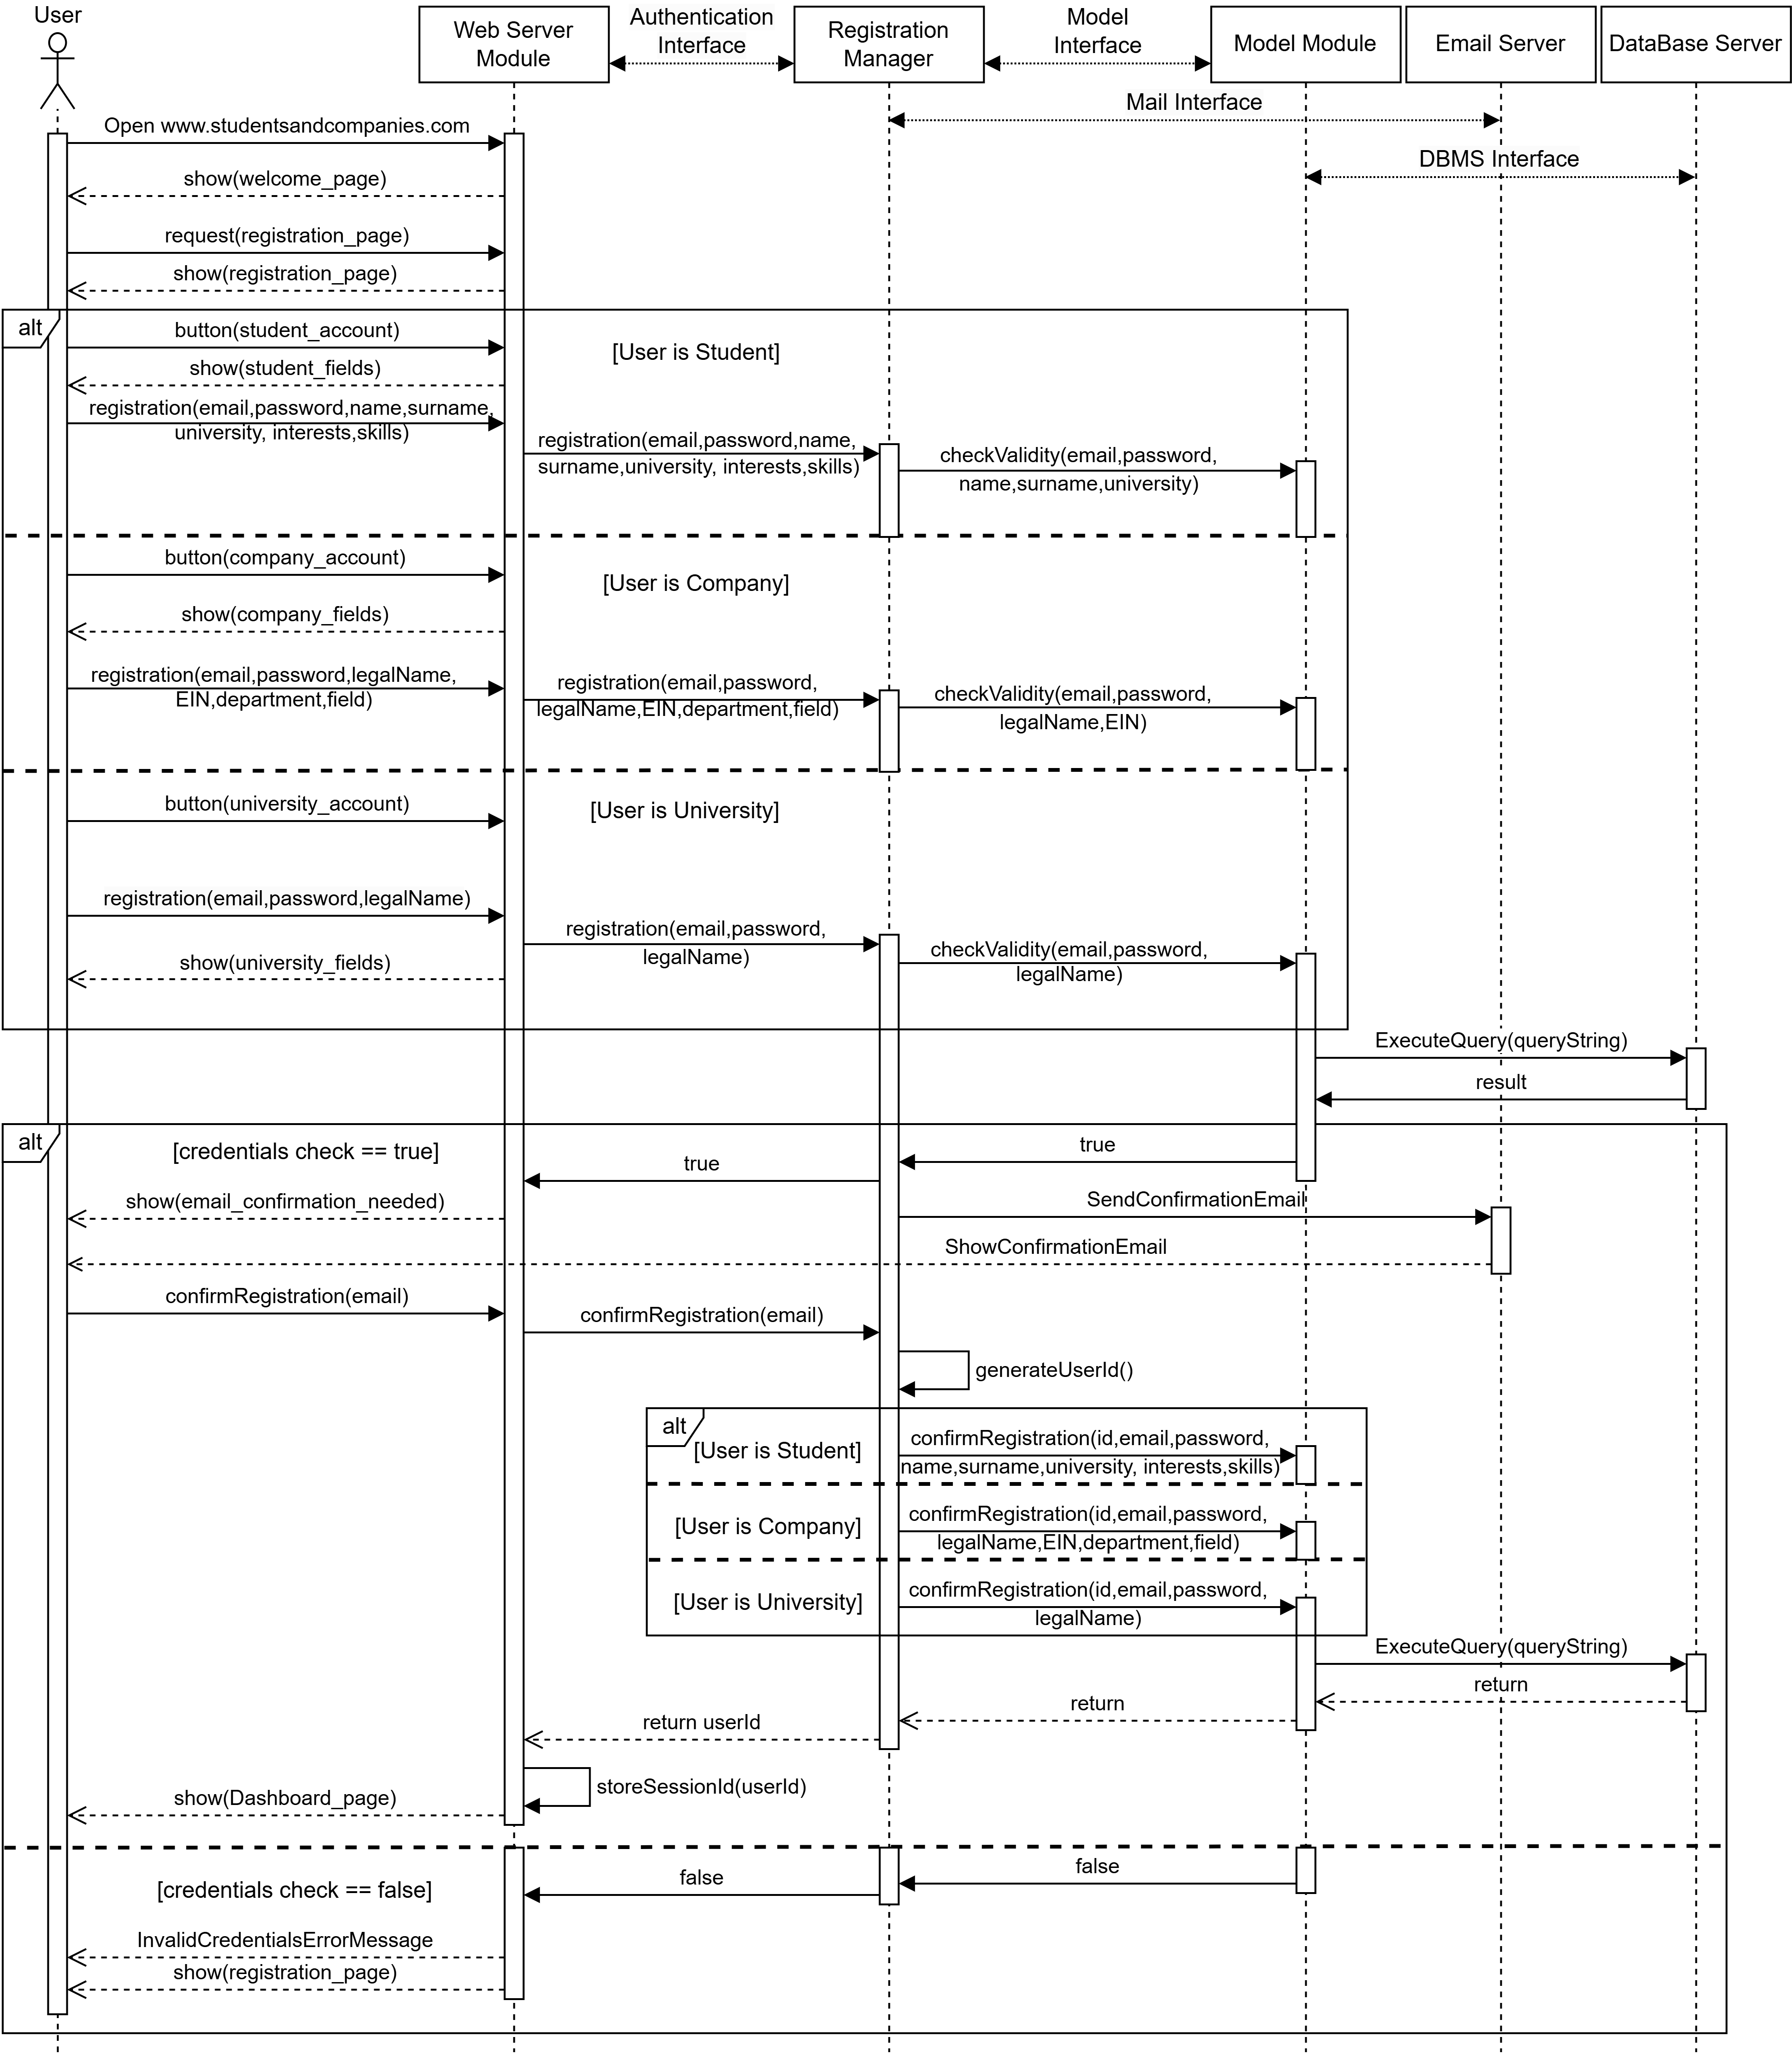
\includegraphics[width=1\textwidth]{Images/Runtime_view/registration_SD.png}
    \caption{Registration to S\&C Sequence Diagram}
\end{figure}
% Use Case 2
\begin{figure}[H]
    \centering
    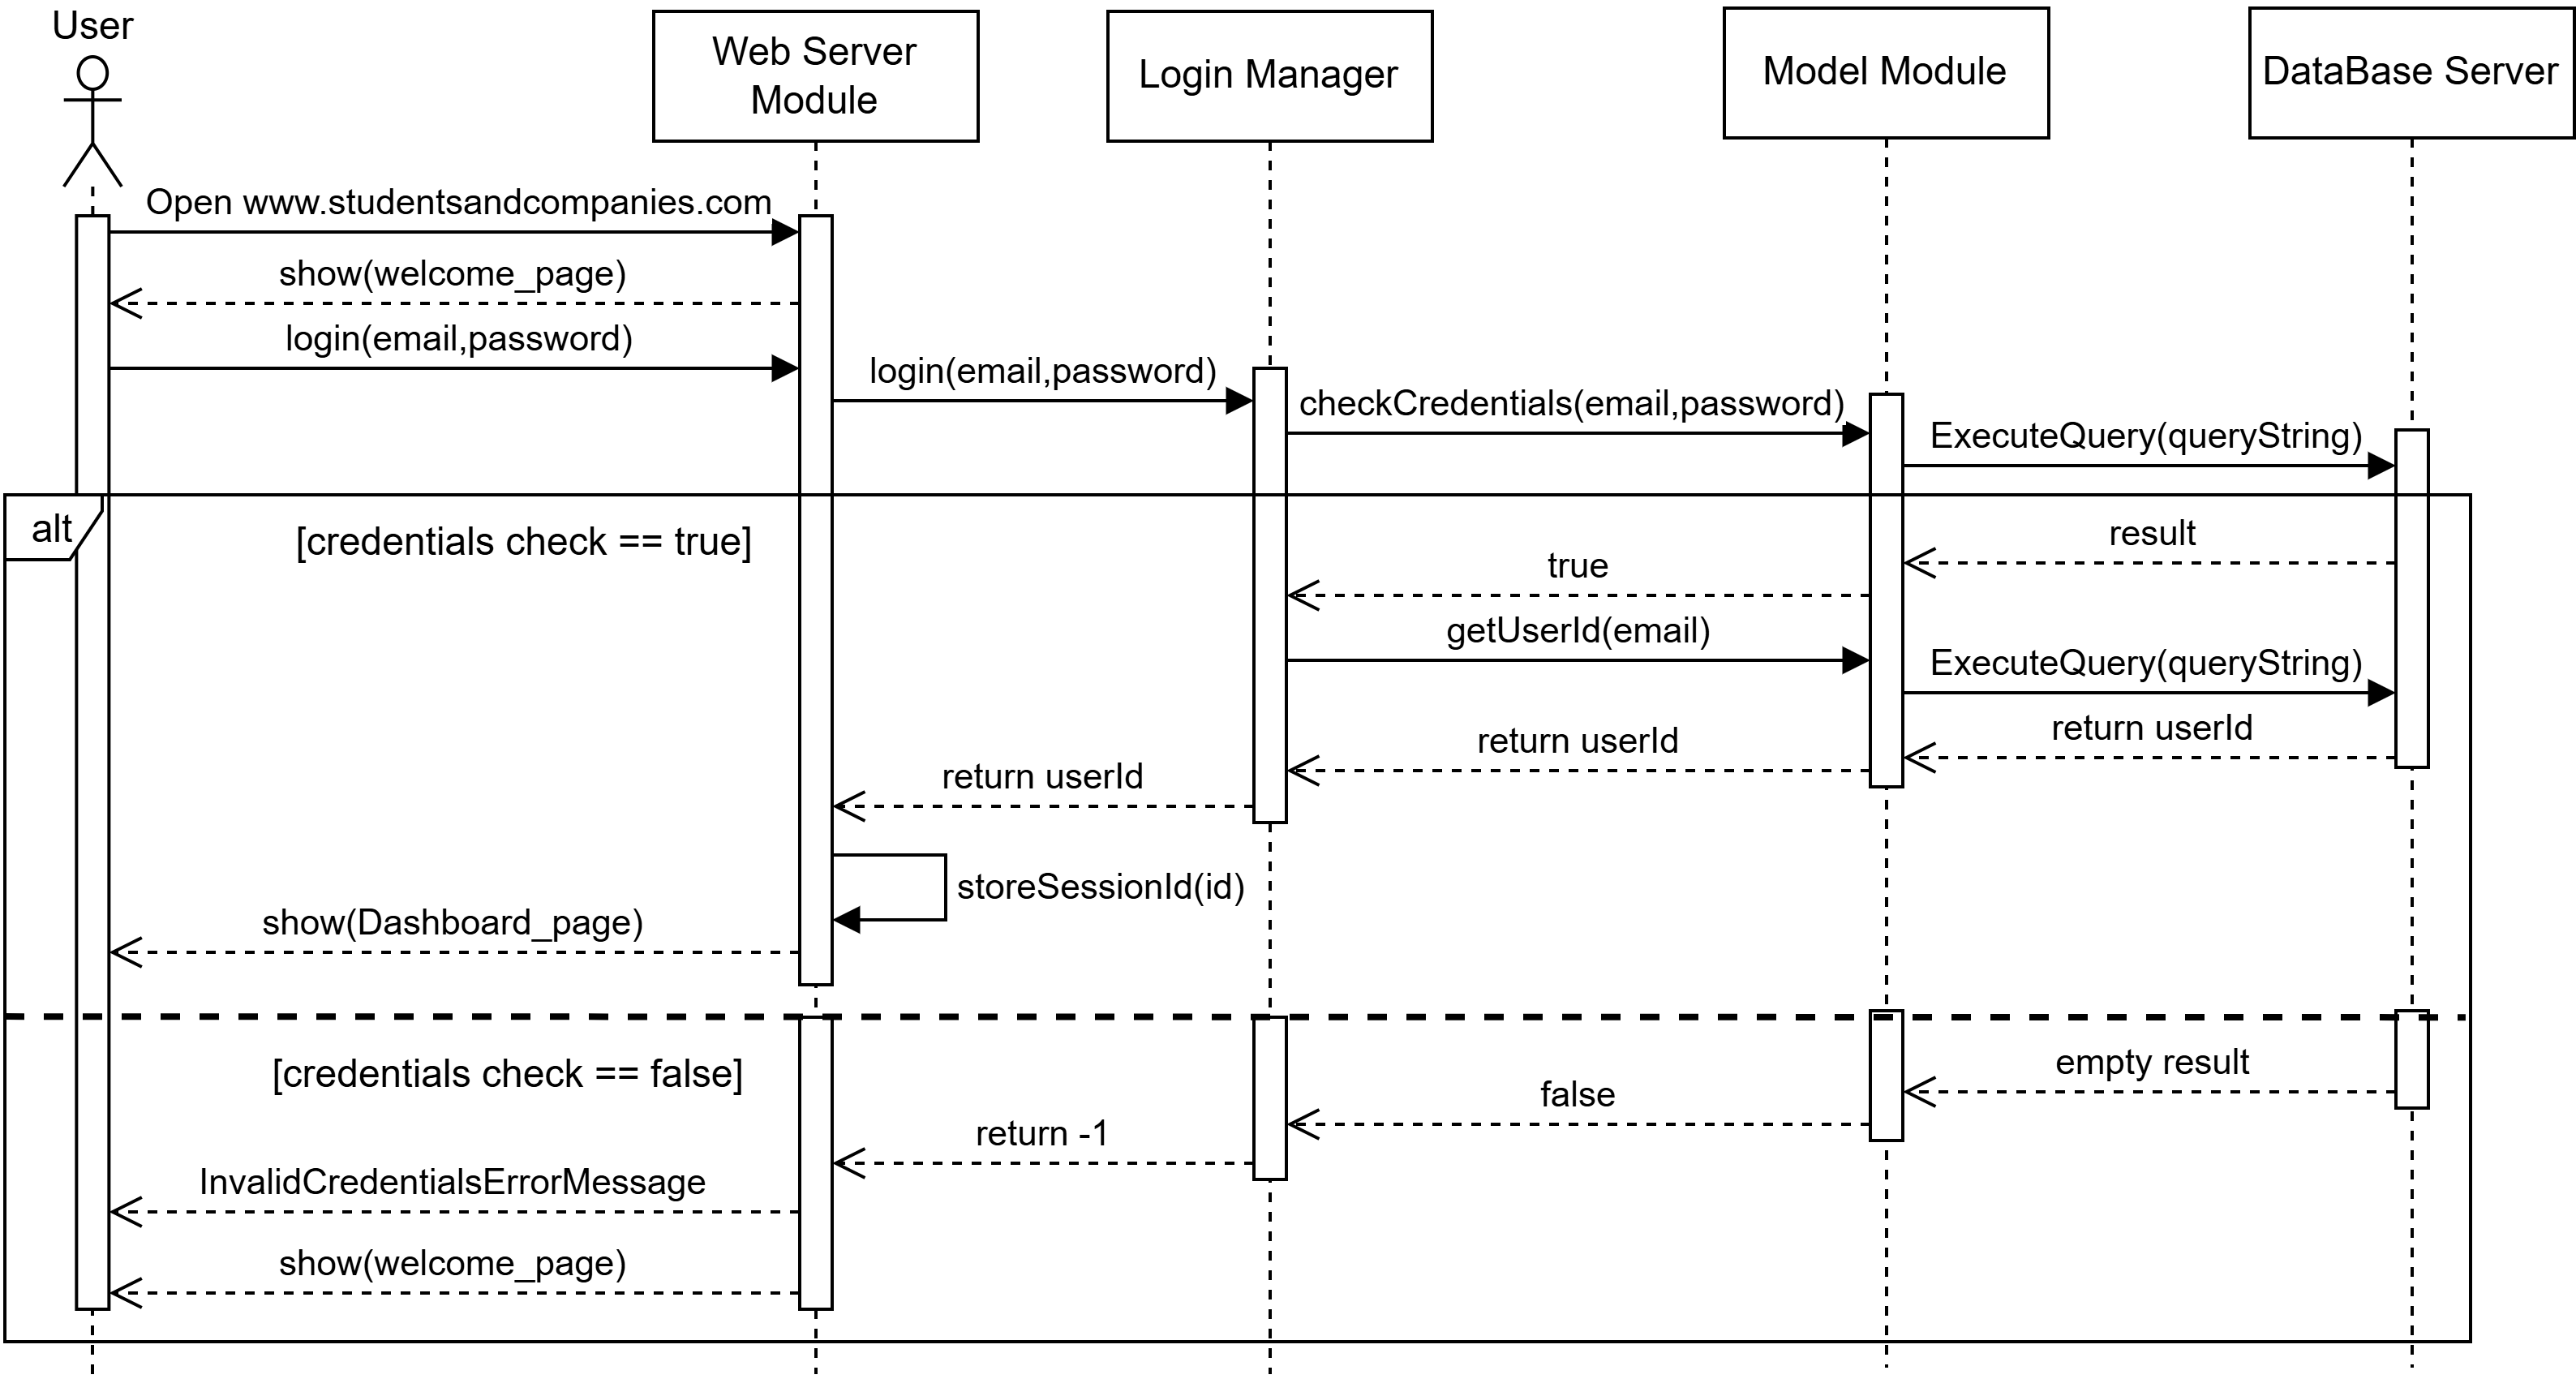
\includegraphics[width=1\textwidth]{Images/Runtime_view/login_SD.png}
    \caption{Login to S\&C Sequence Diagram}
\end{figure}
% Use Case 3
\begin{figure}[H]
    \centering
    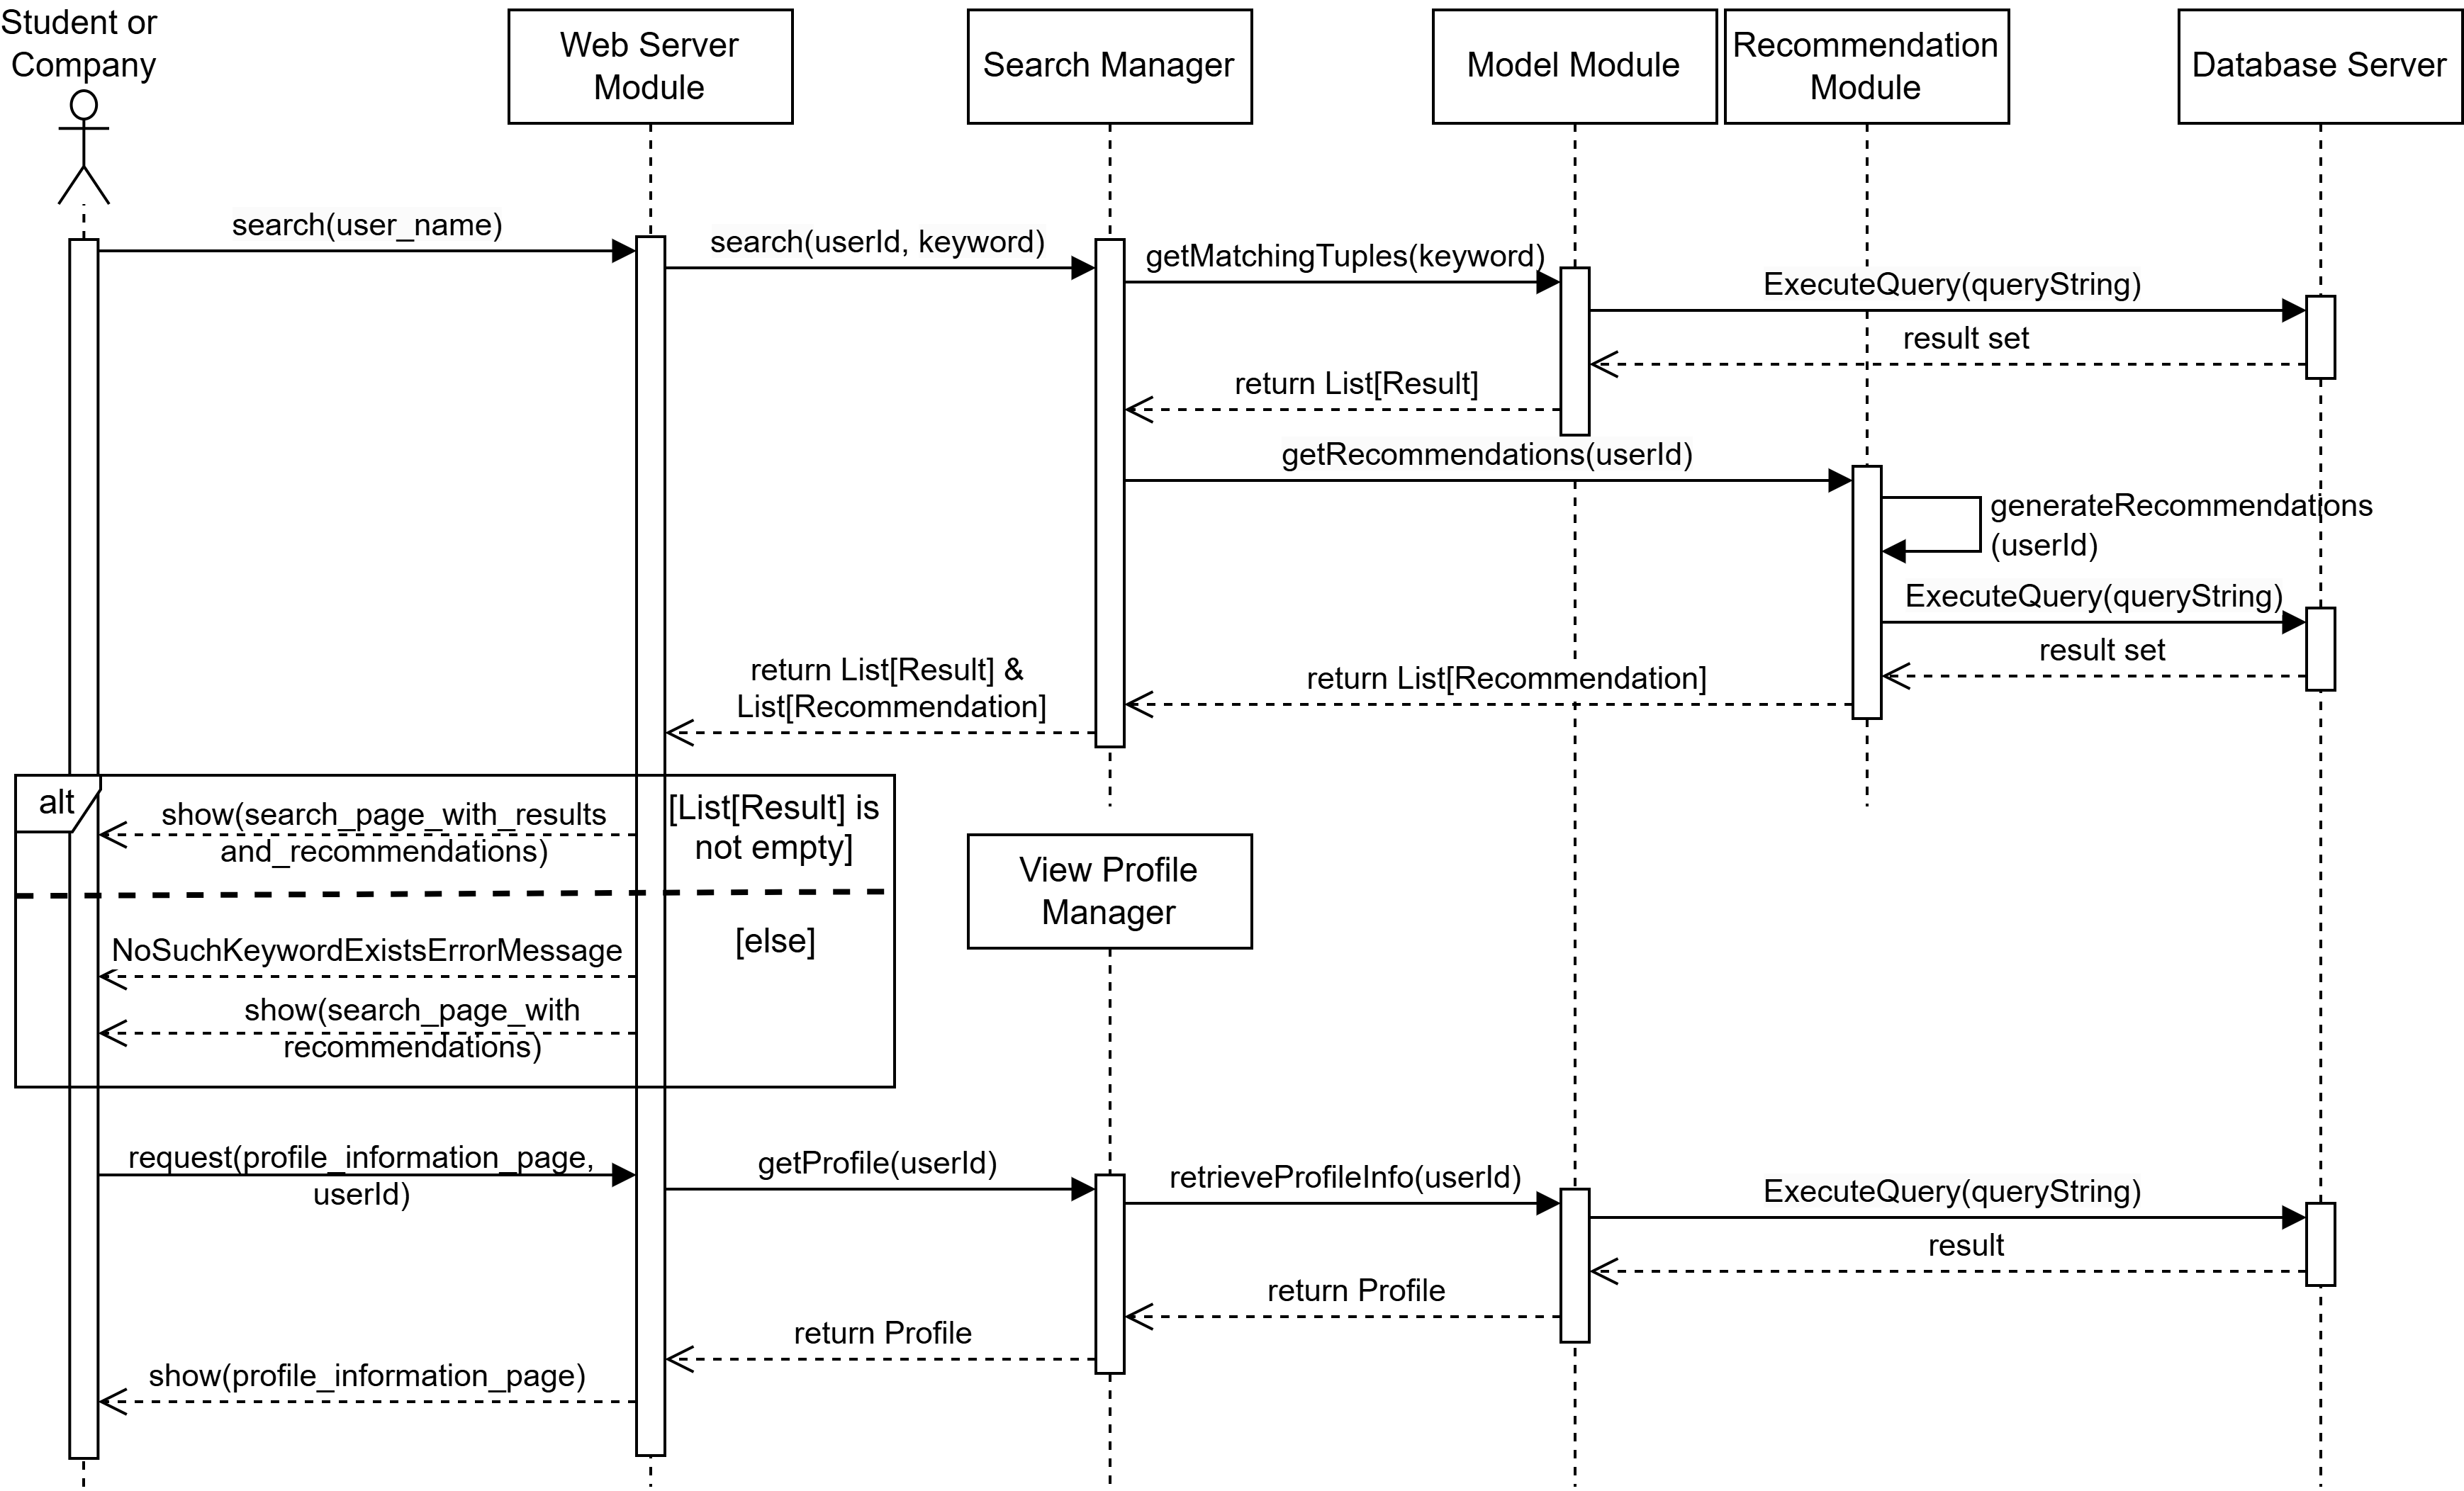
\includegraphics[width=1\textwidth]{Images/Runtime_view/seeProfile_SD.png}
    \caption{User sees profile information Sequence Diagram}
\end{figure}
% Use Case 4
\begin{figure}[H]
    \centering
    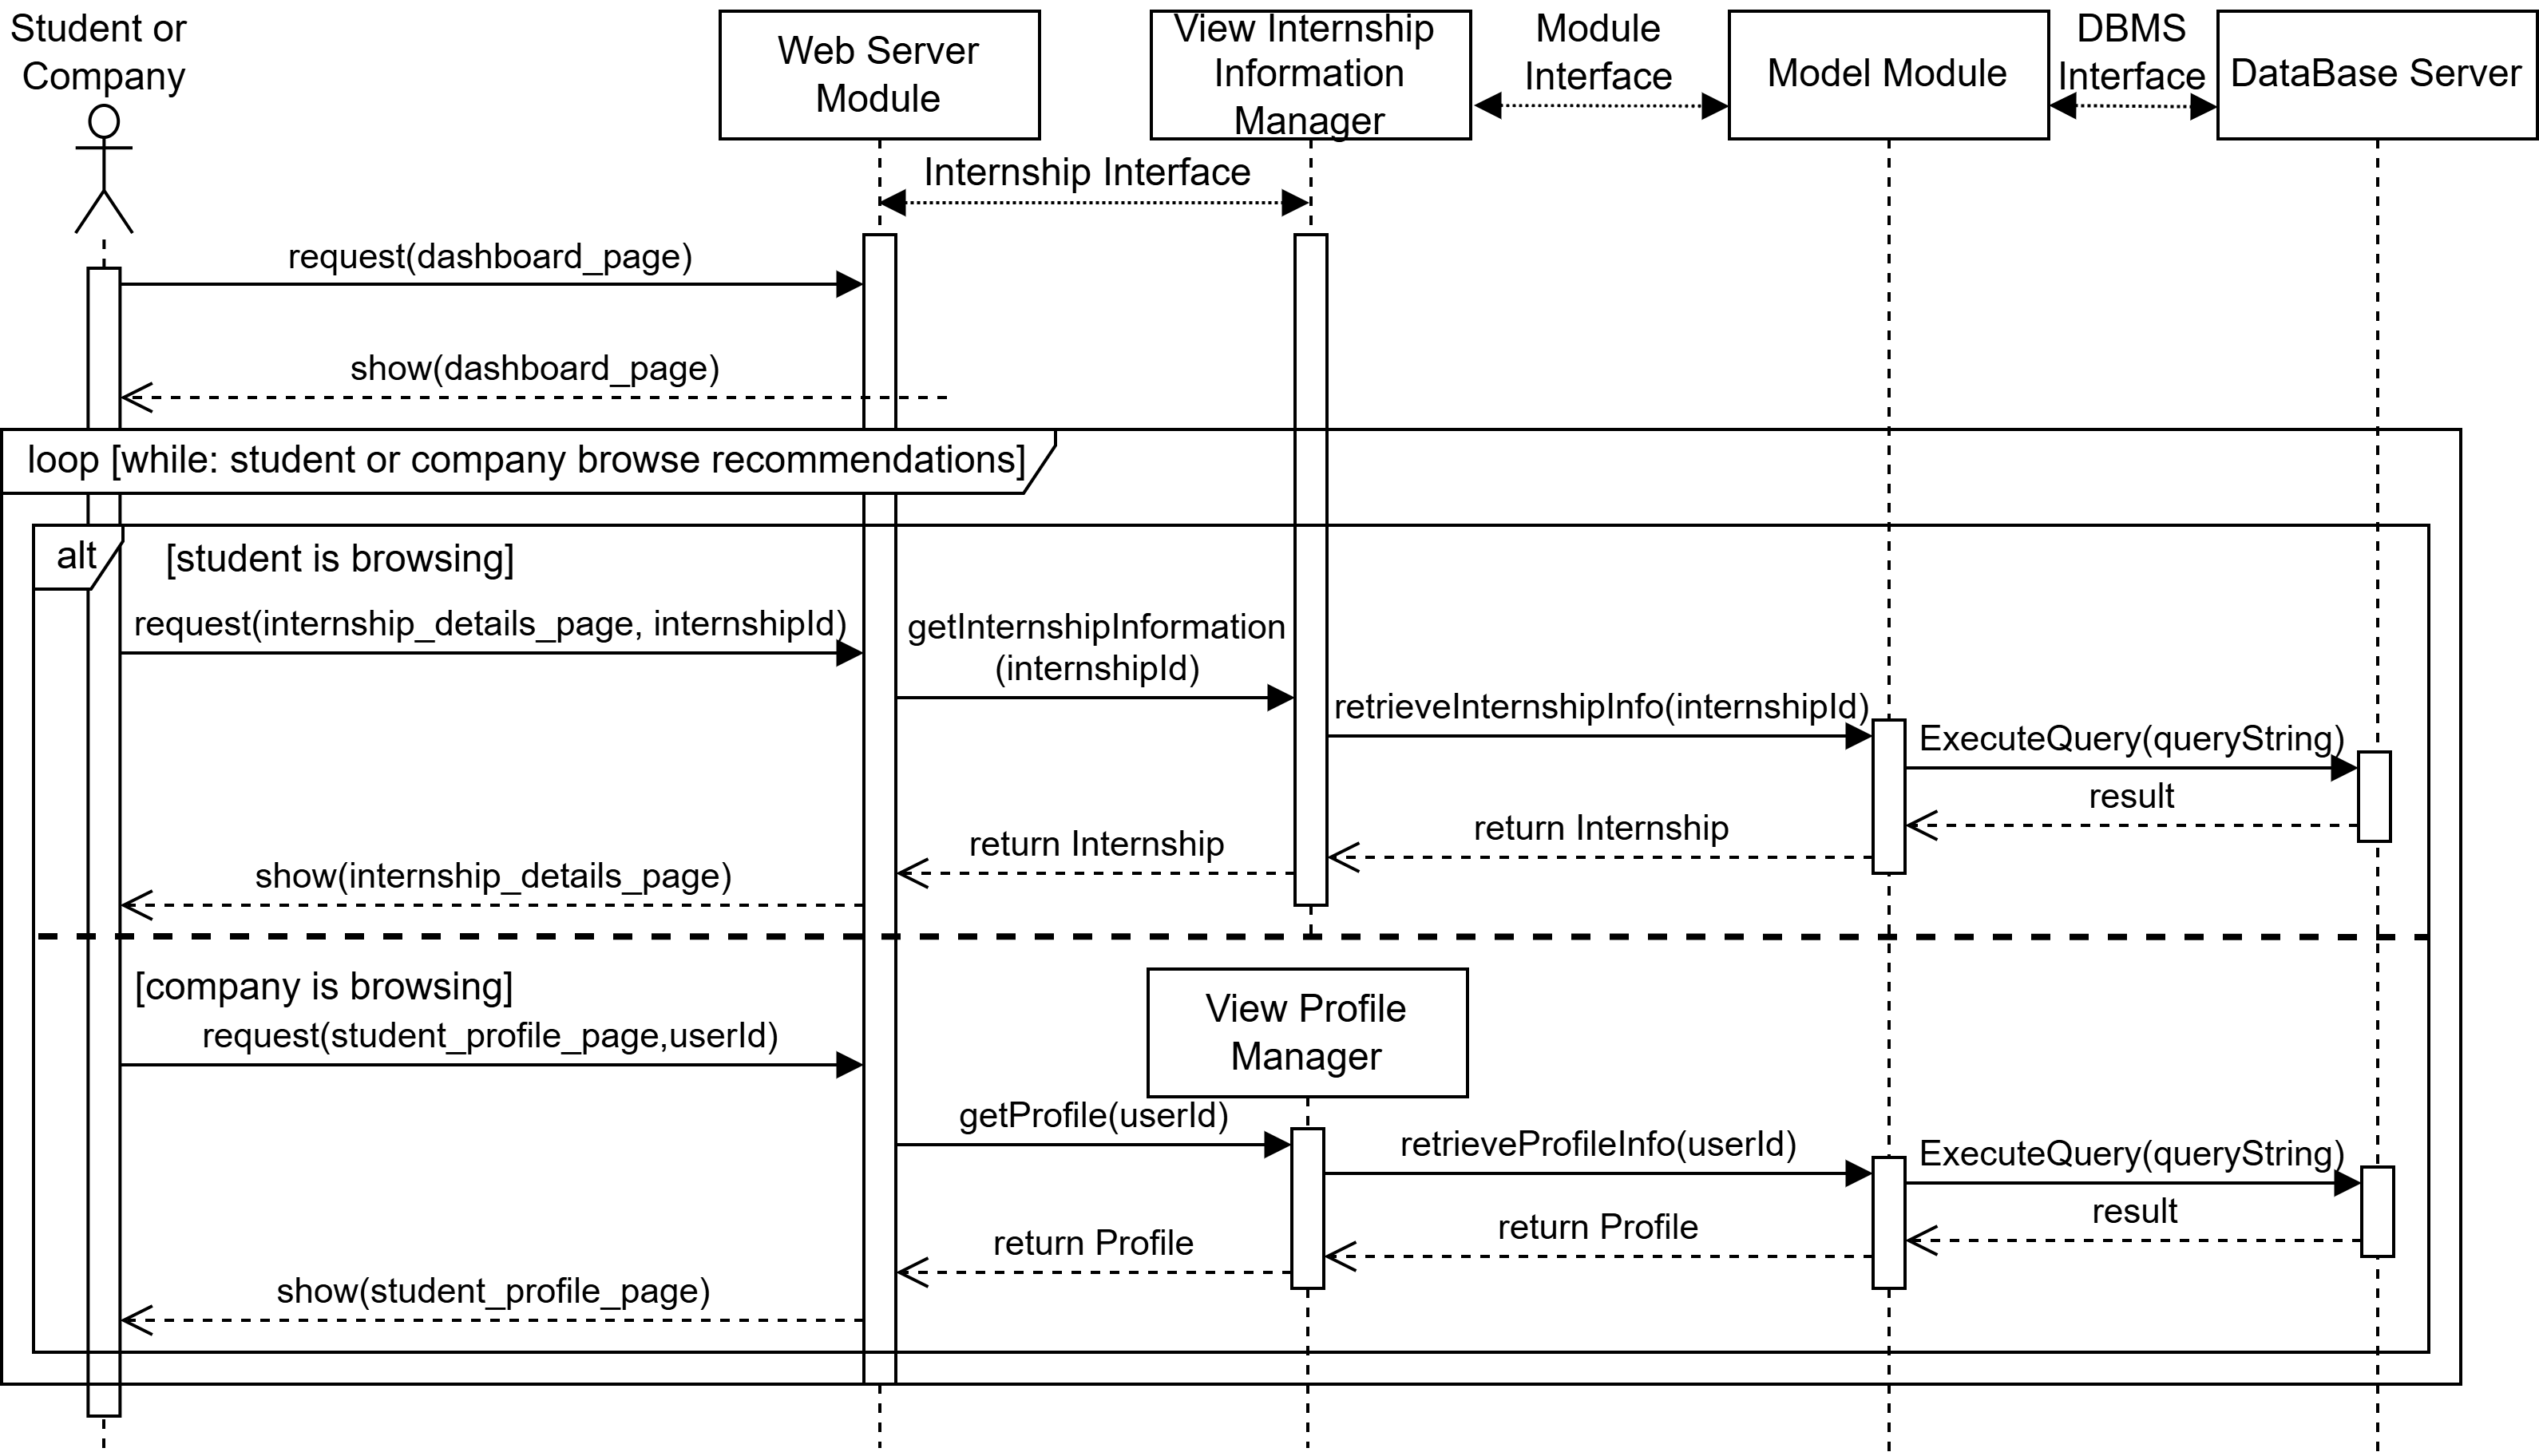
\includegraphics[width=1\textwidth]{Images/Runtime_view/recommendation_SD.png}
    \caption{Student or Company views recommendation Sequence Diagram}
\end{figure}
% Use Case 5
\begin{figure}[H]
    \centering
    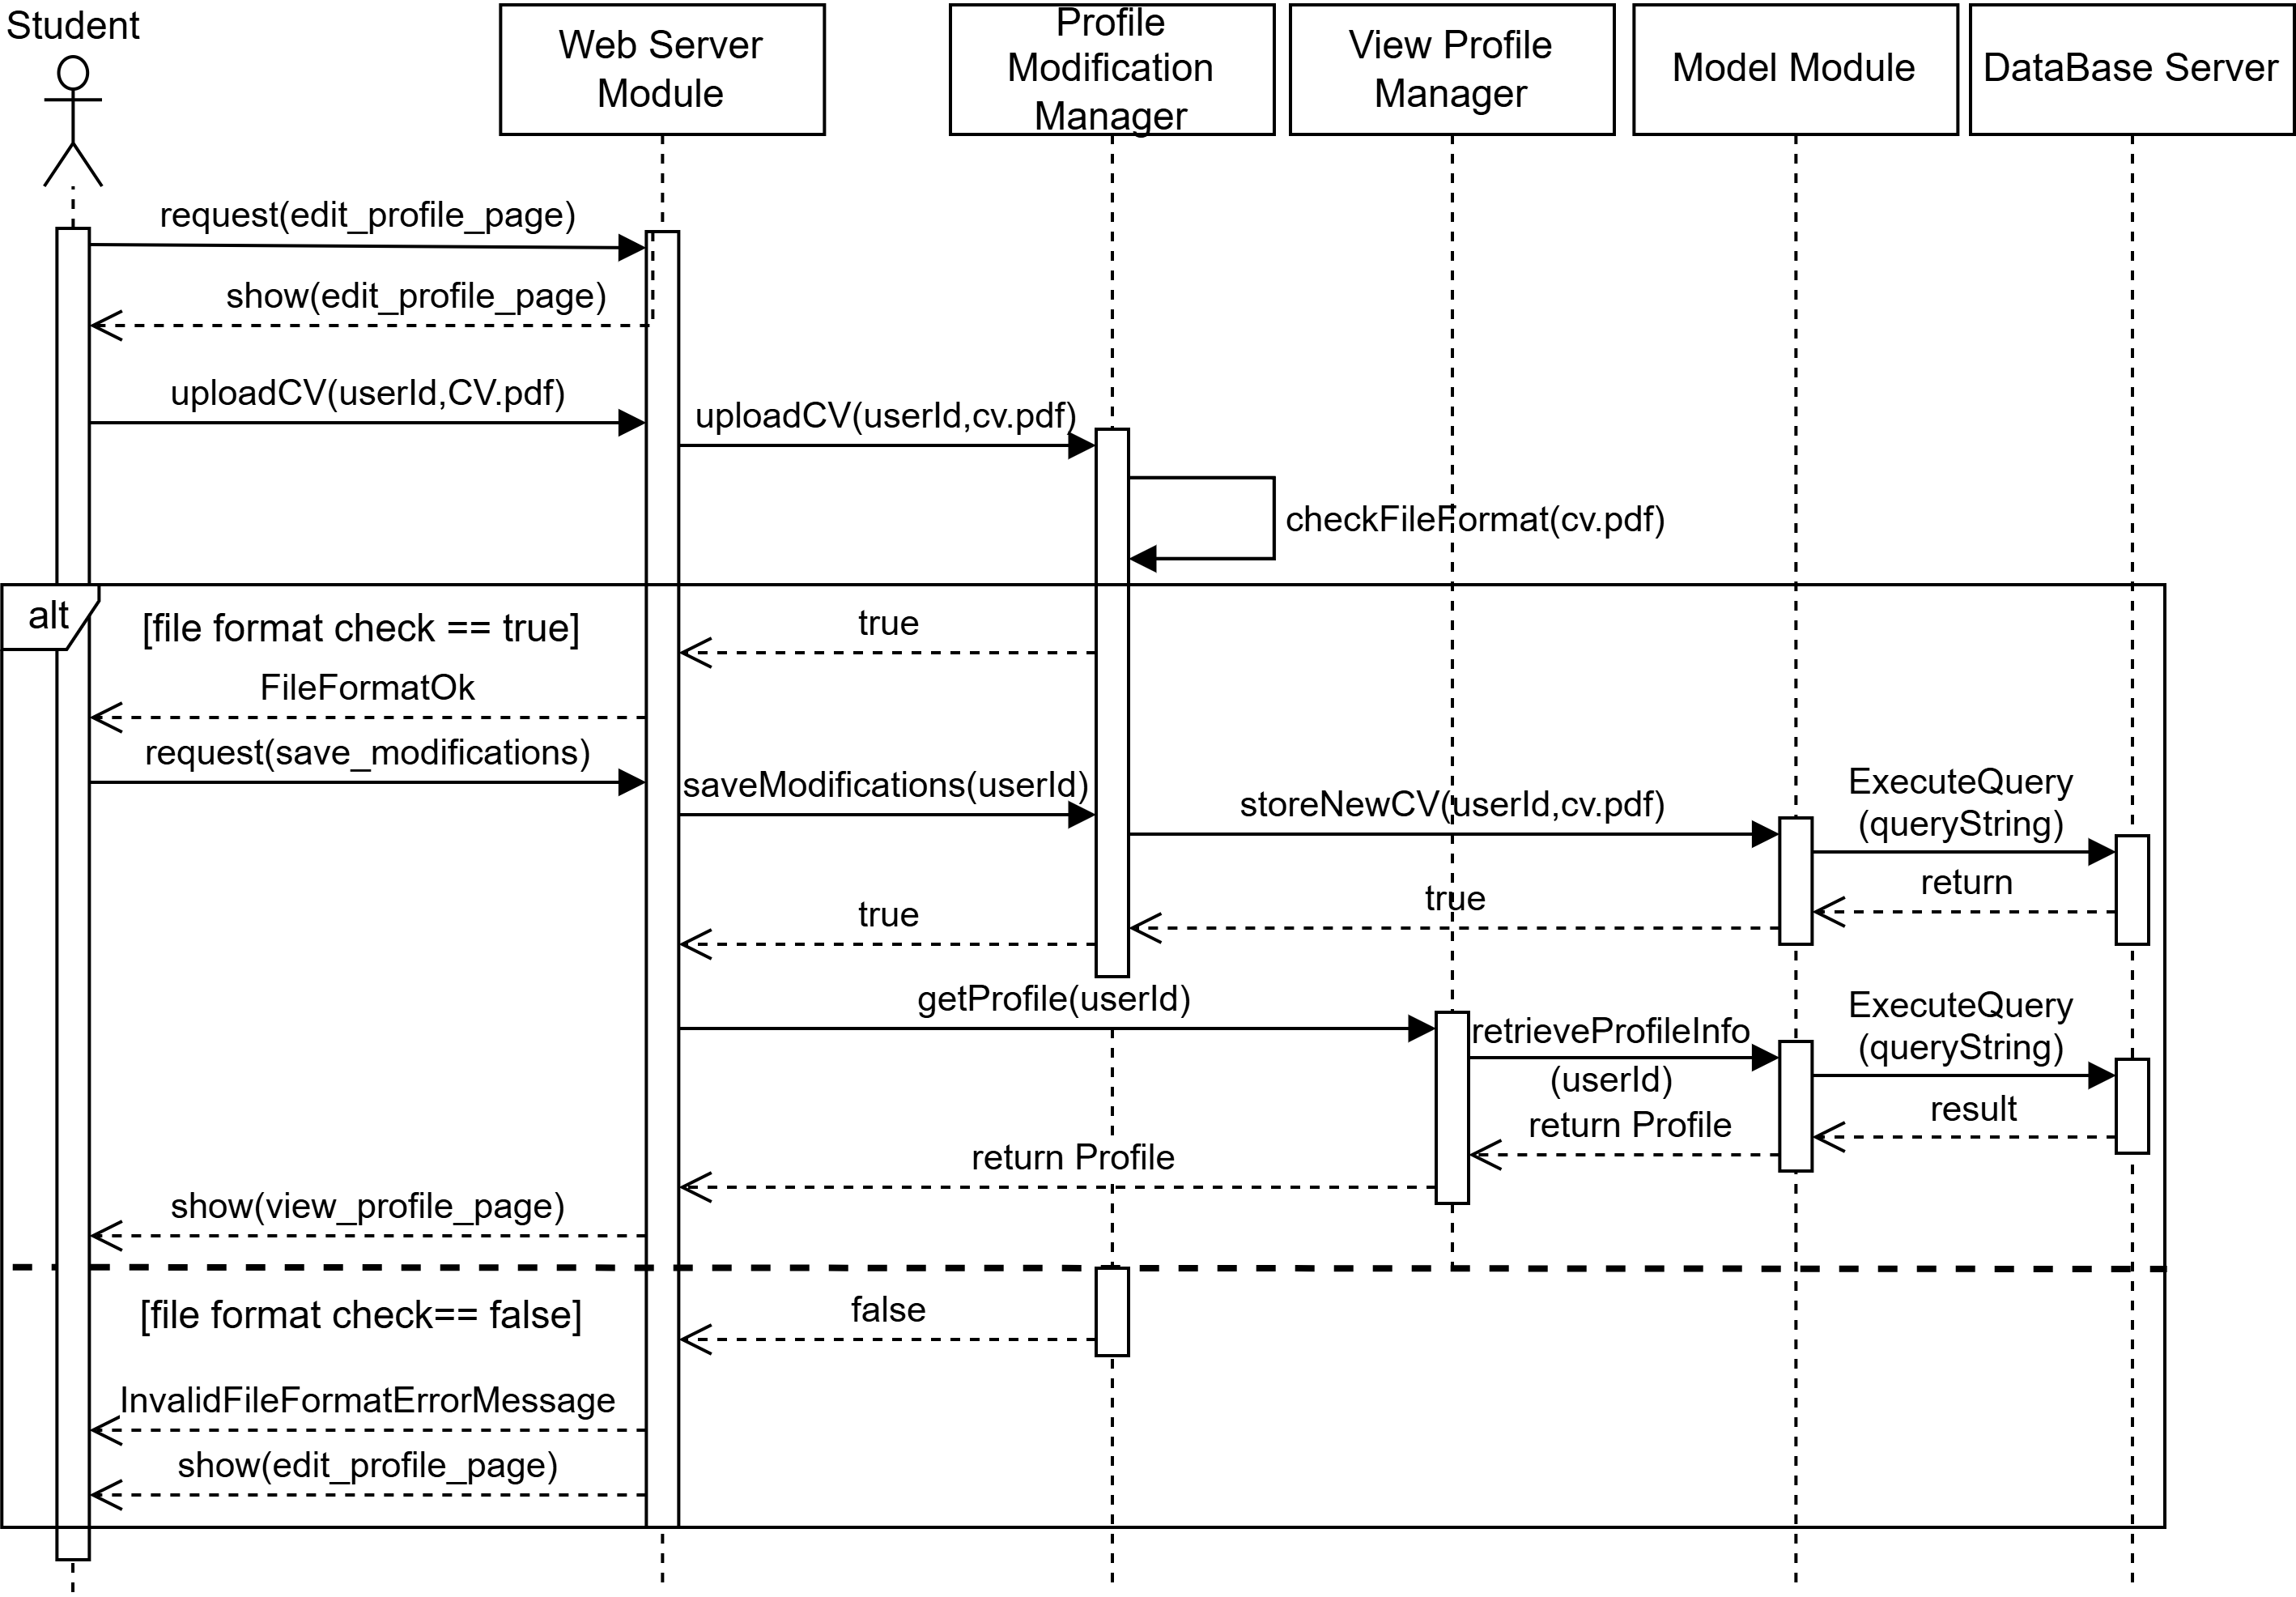
\includegraphics[width=1\textwidth]{Images/Runtime_view/uploadCV_SD.png}
    \caption{Student uploads CV to his profile Sequence Diagram}
\end{figure}
% Use Case 6
\begin{figure}[H]
    \centering
    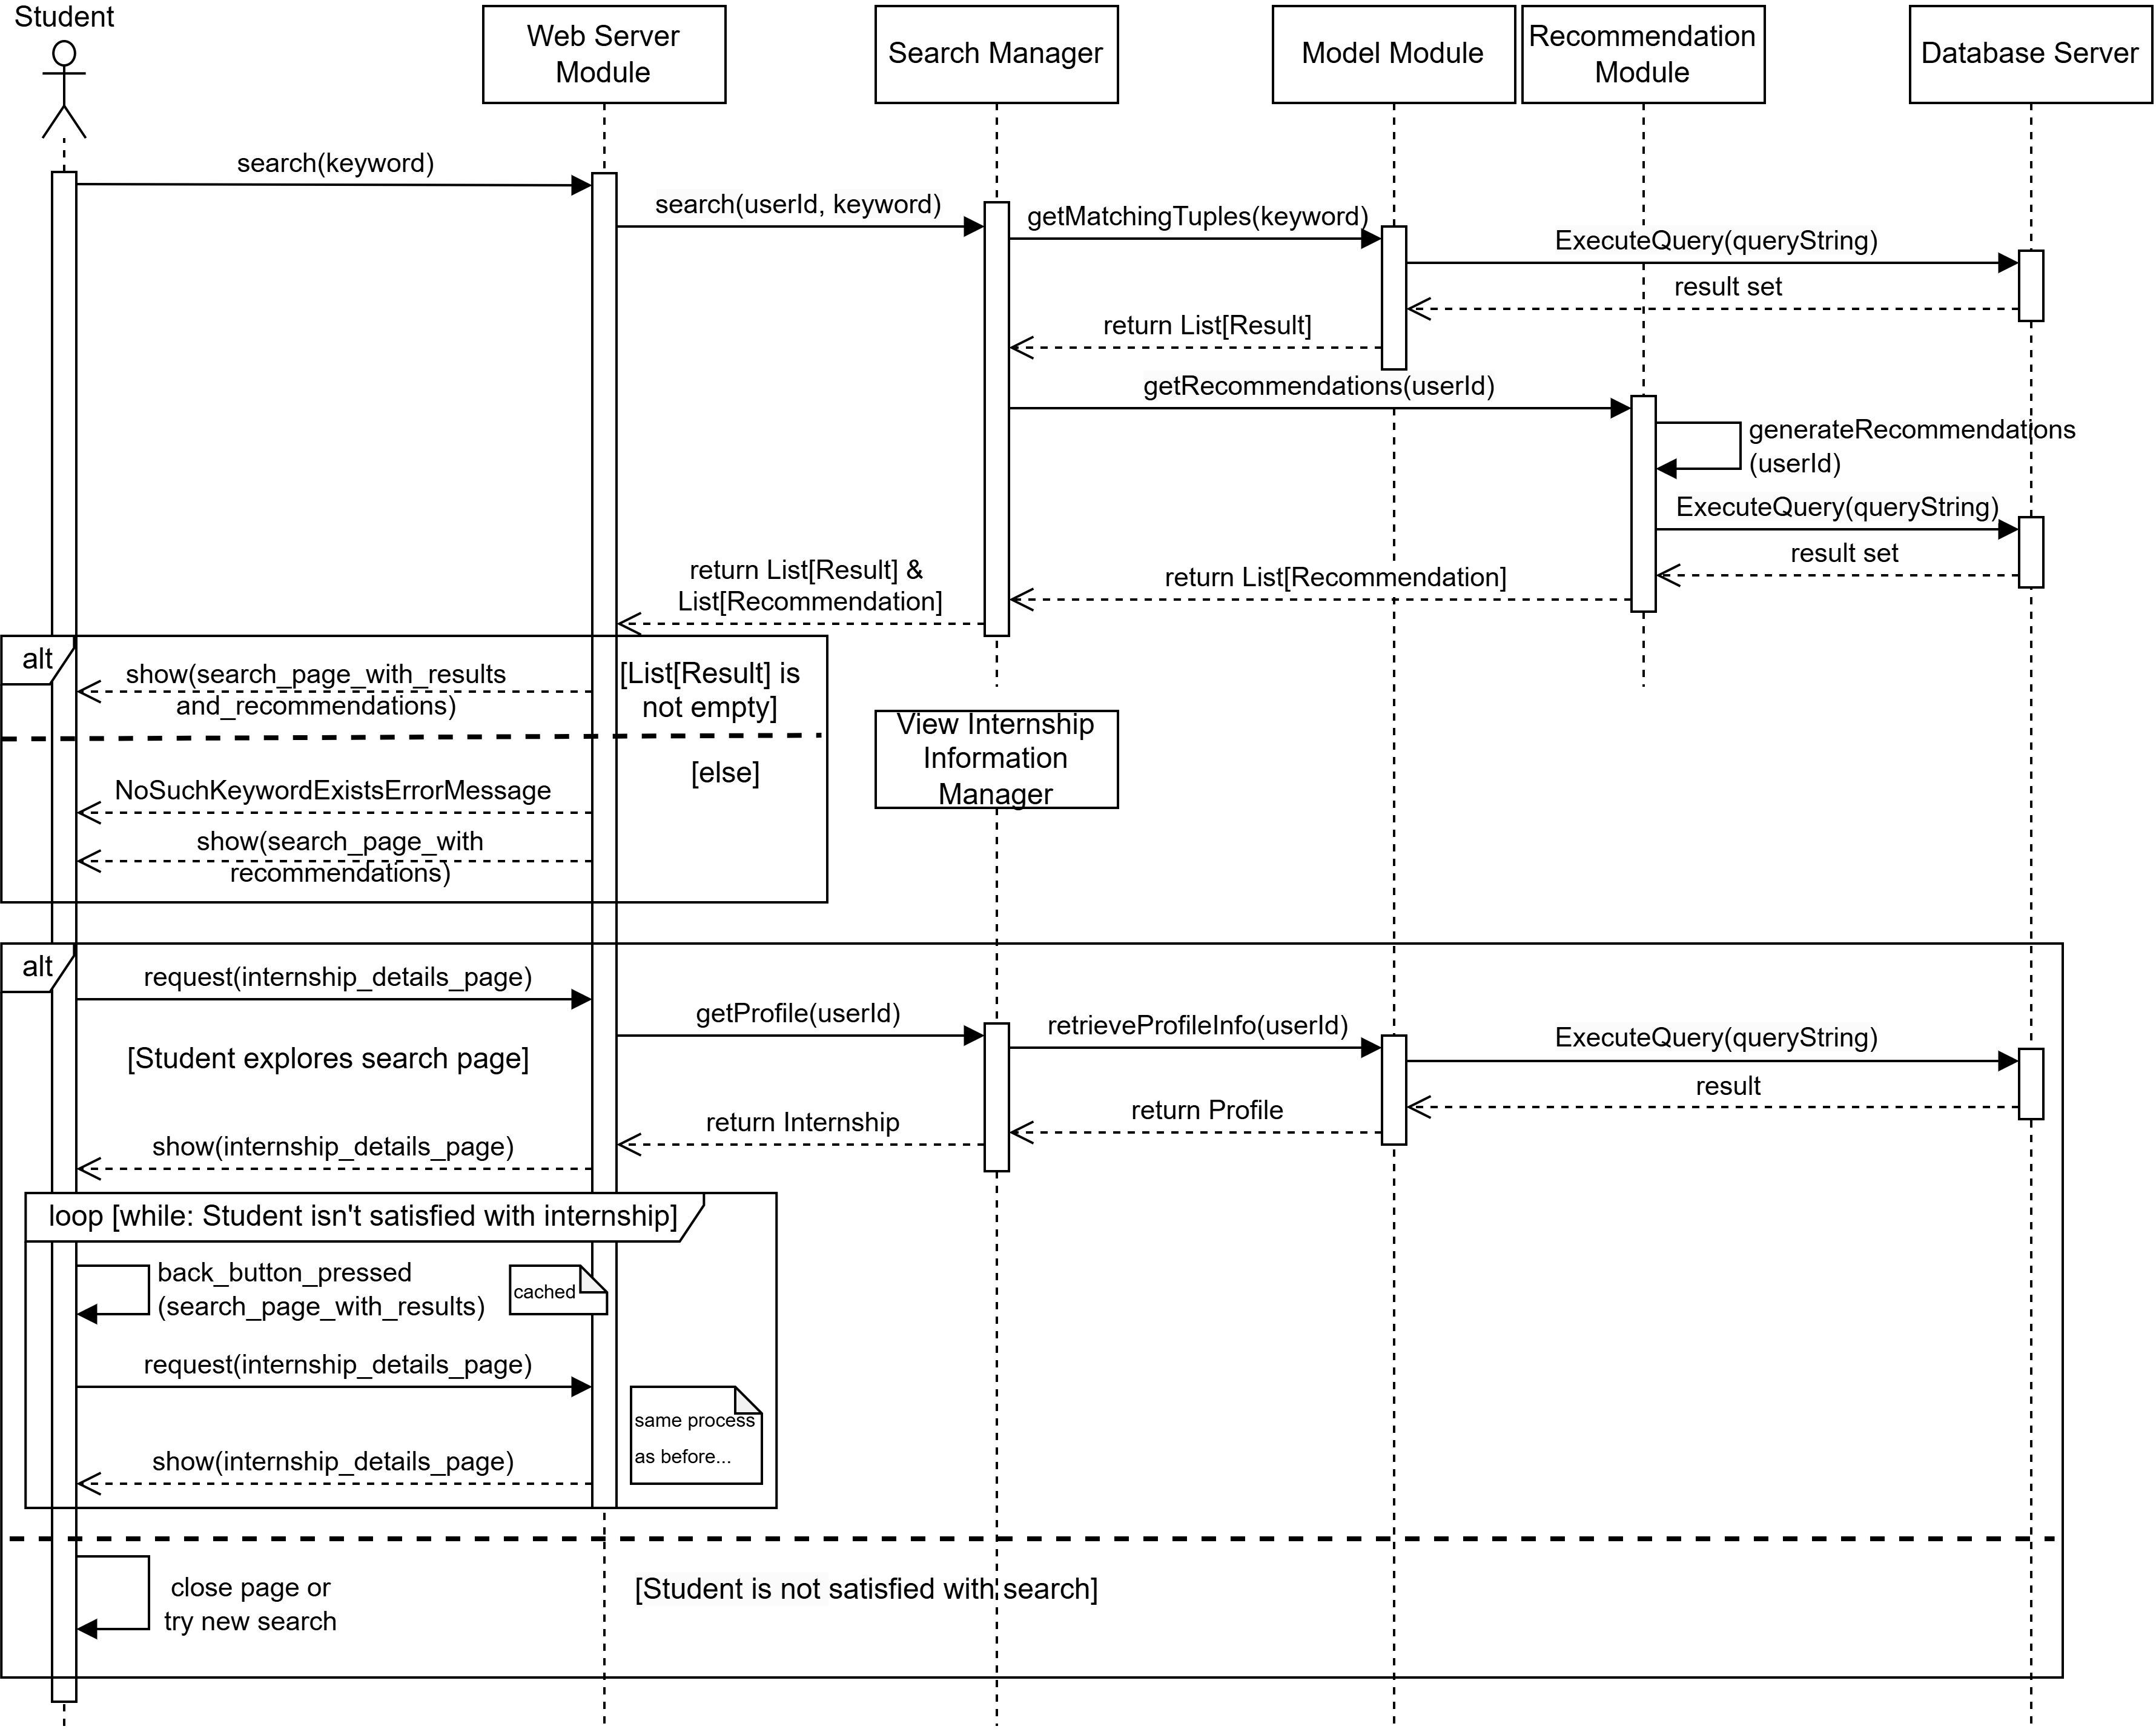
\includegraphics[width=1\textwidth]{Images/Runtime_view/searchInt_SD.png}
    \caption{Student searches for an internship Sequence Diagram}
\end{figure}
% Use Case 7
\begin{figure}[H]
    \centering
    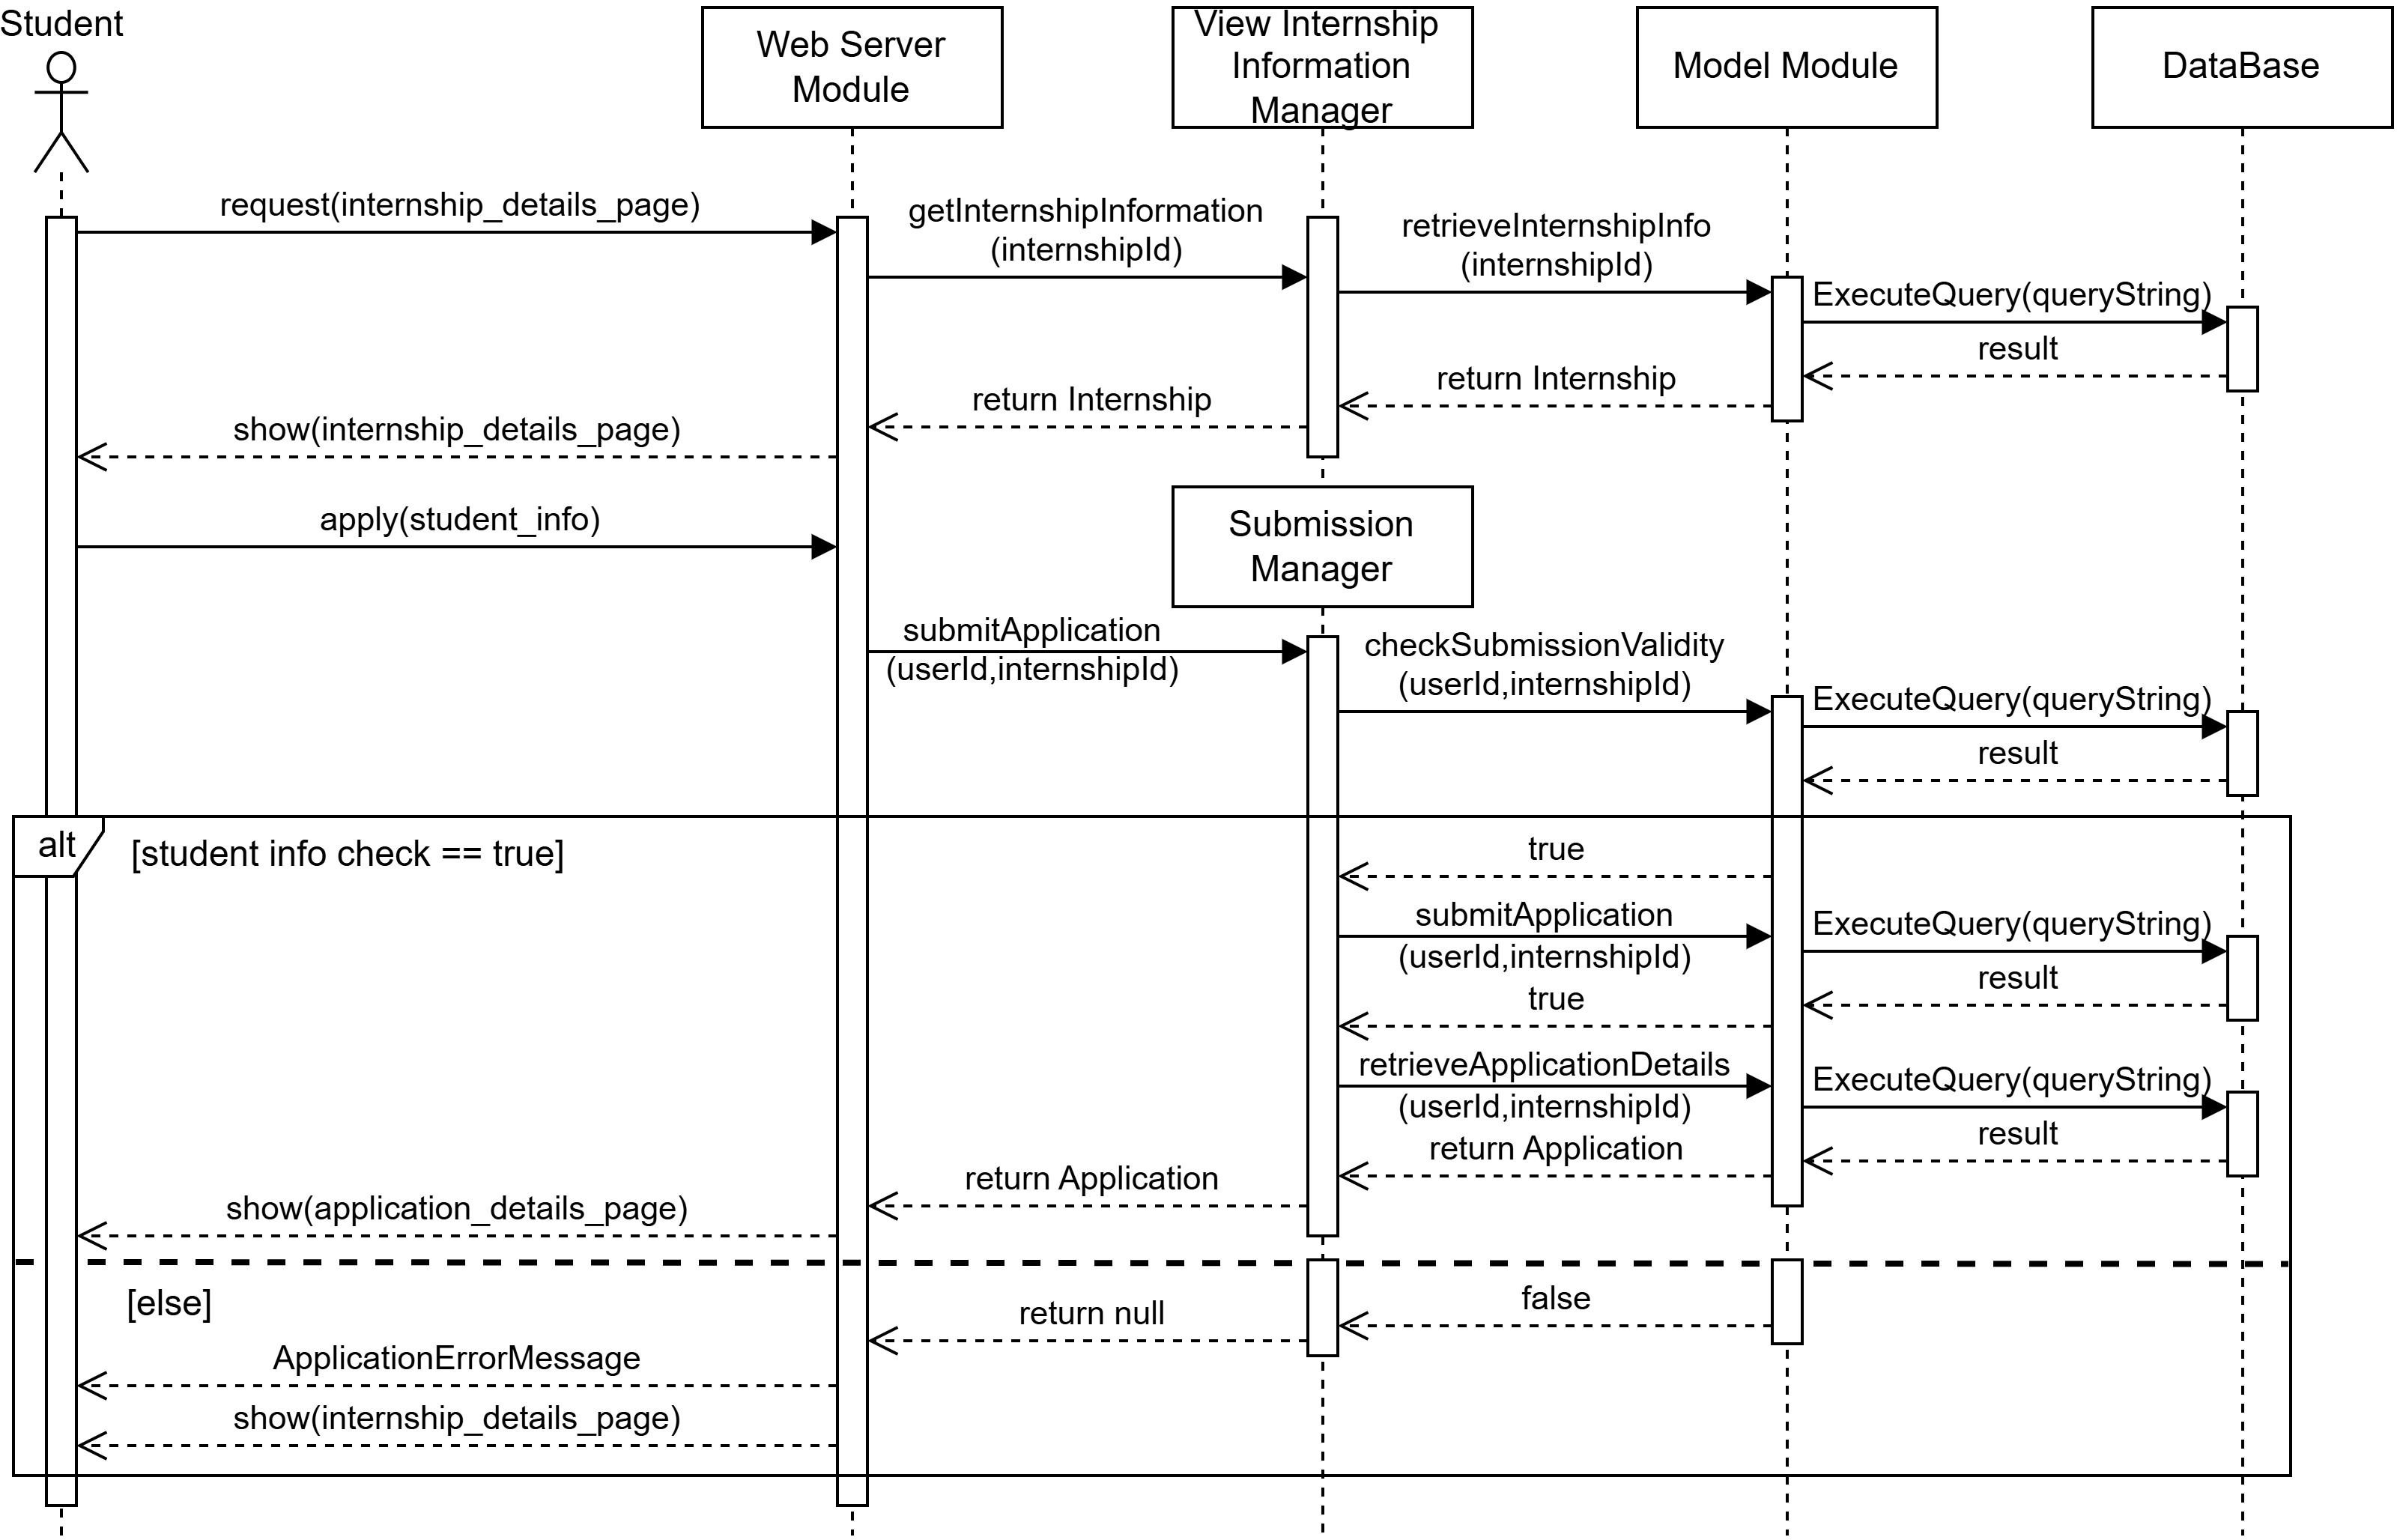
\includegraphics[width=1\textwidth]{Images/Runtime_view/applyInt_SD.png}
    \caption{Student applies for an internship Sequence Diagram}
\end{figure}
% Use Case 8
\begin{figure}[H]
    \centering
    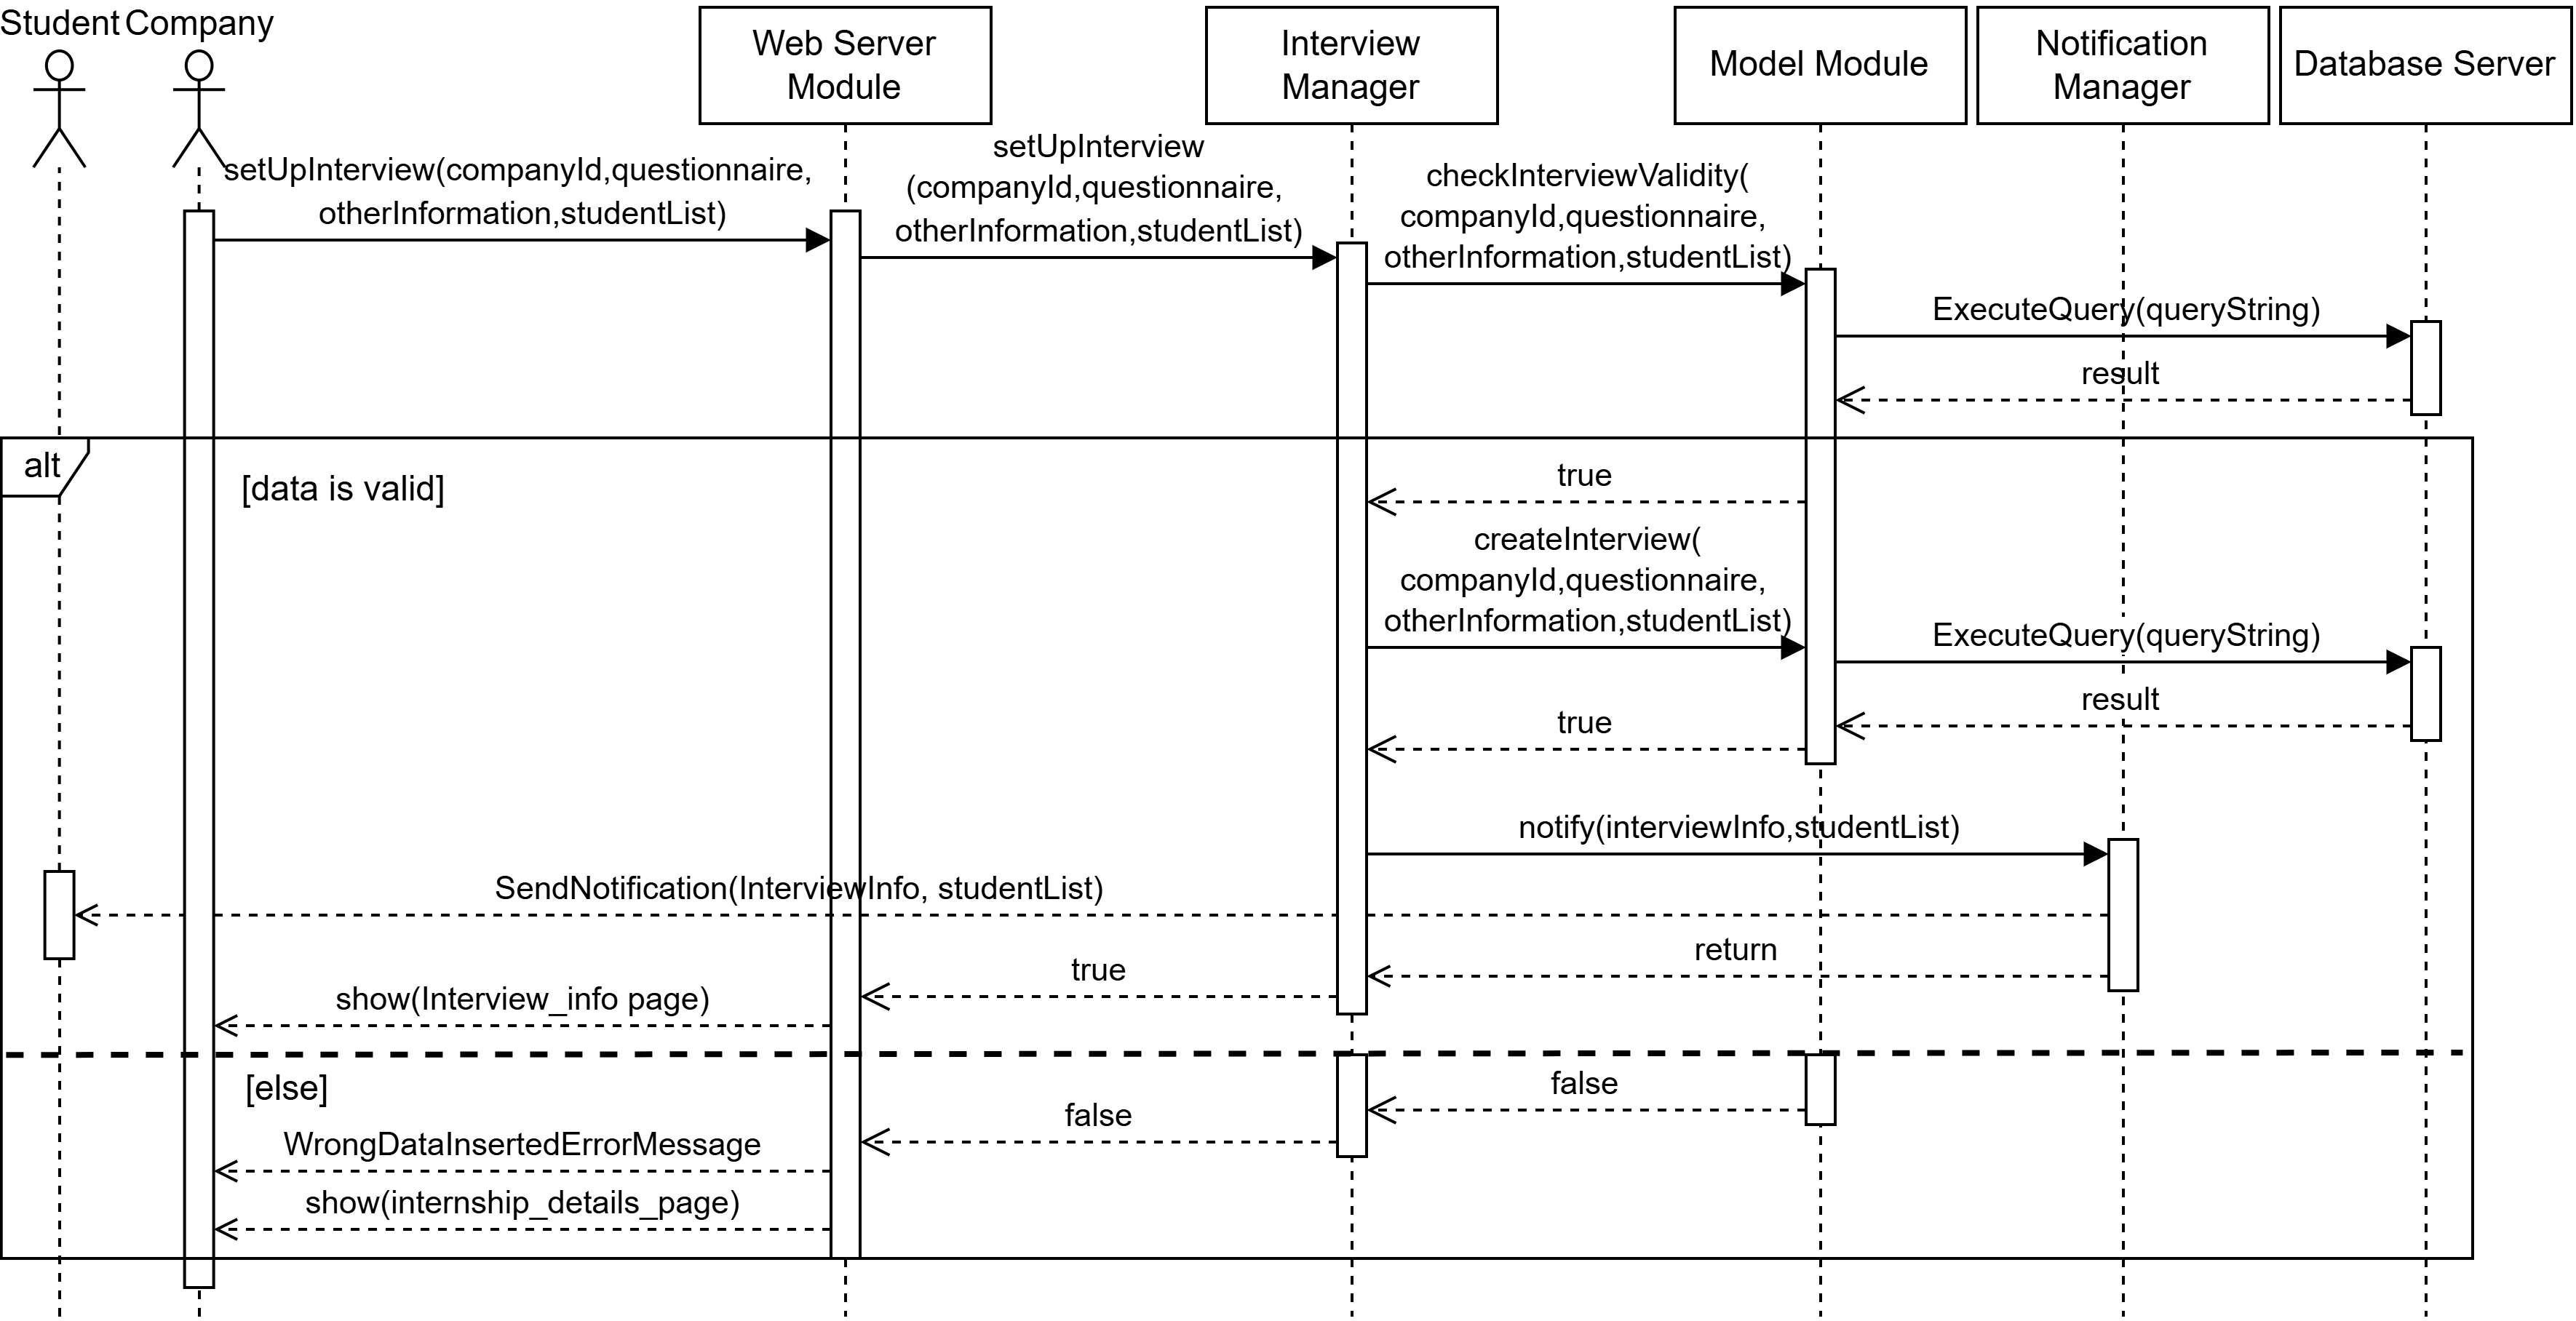
\includegraphics[width=1\textwidth]{Images/Runtime_view/createIntvw_SD.png}
    \caption{Company creates an interview Sequence Diagram}
\end{figure}
% Use Case 9
\begin{figure}[H]
    \centering
    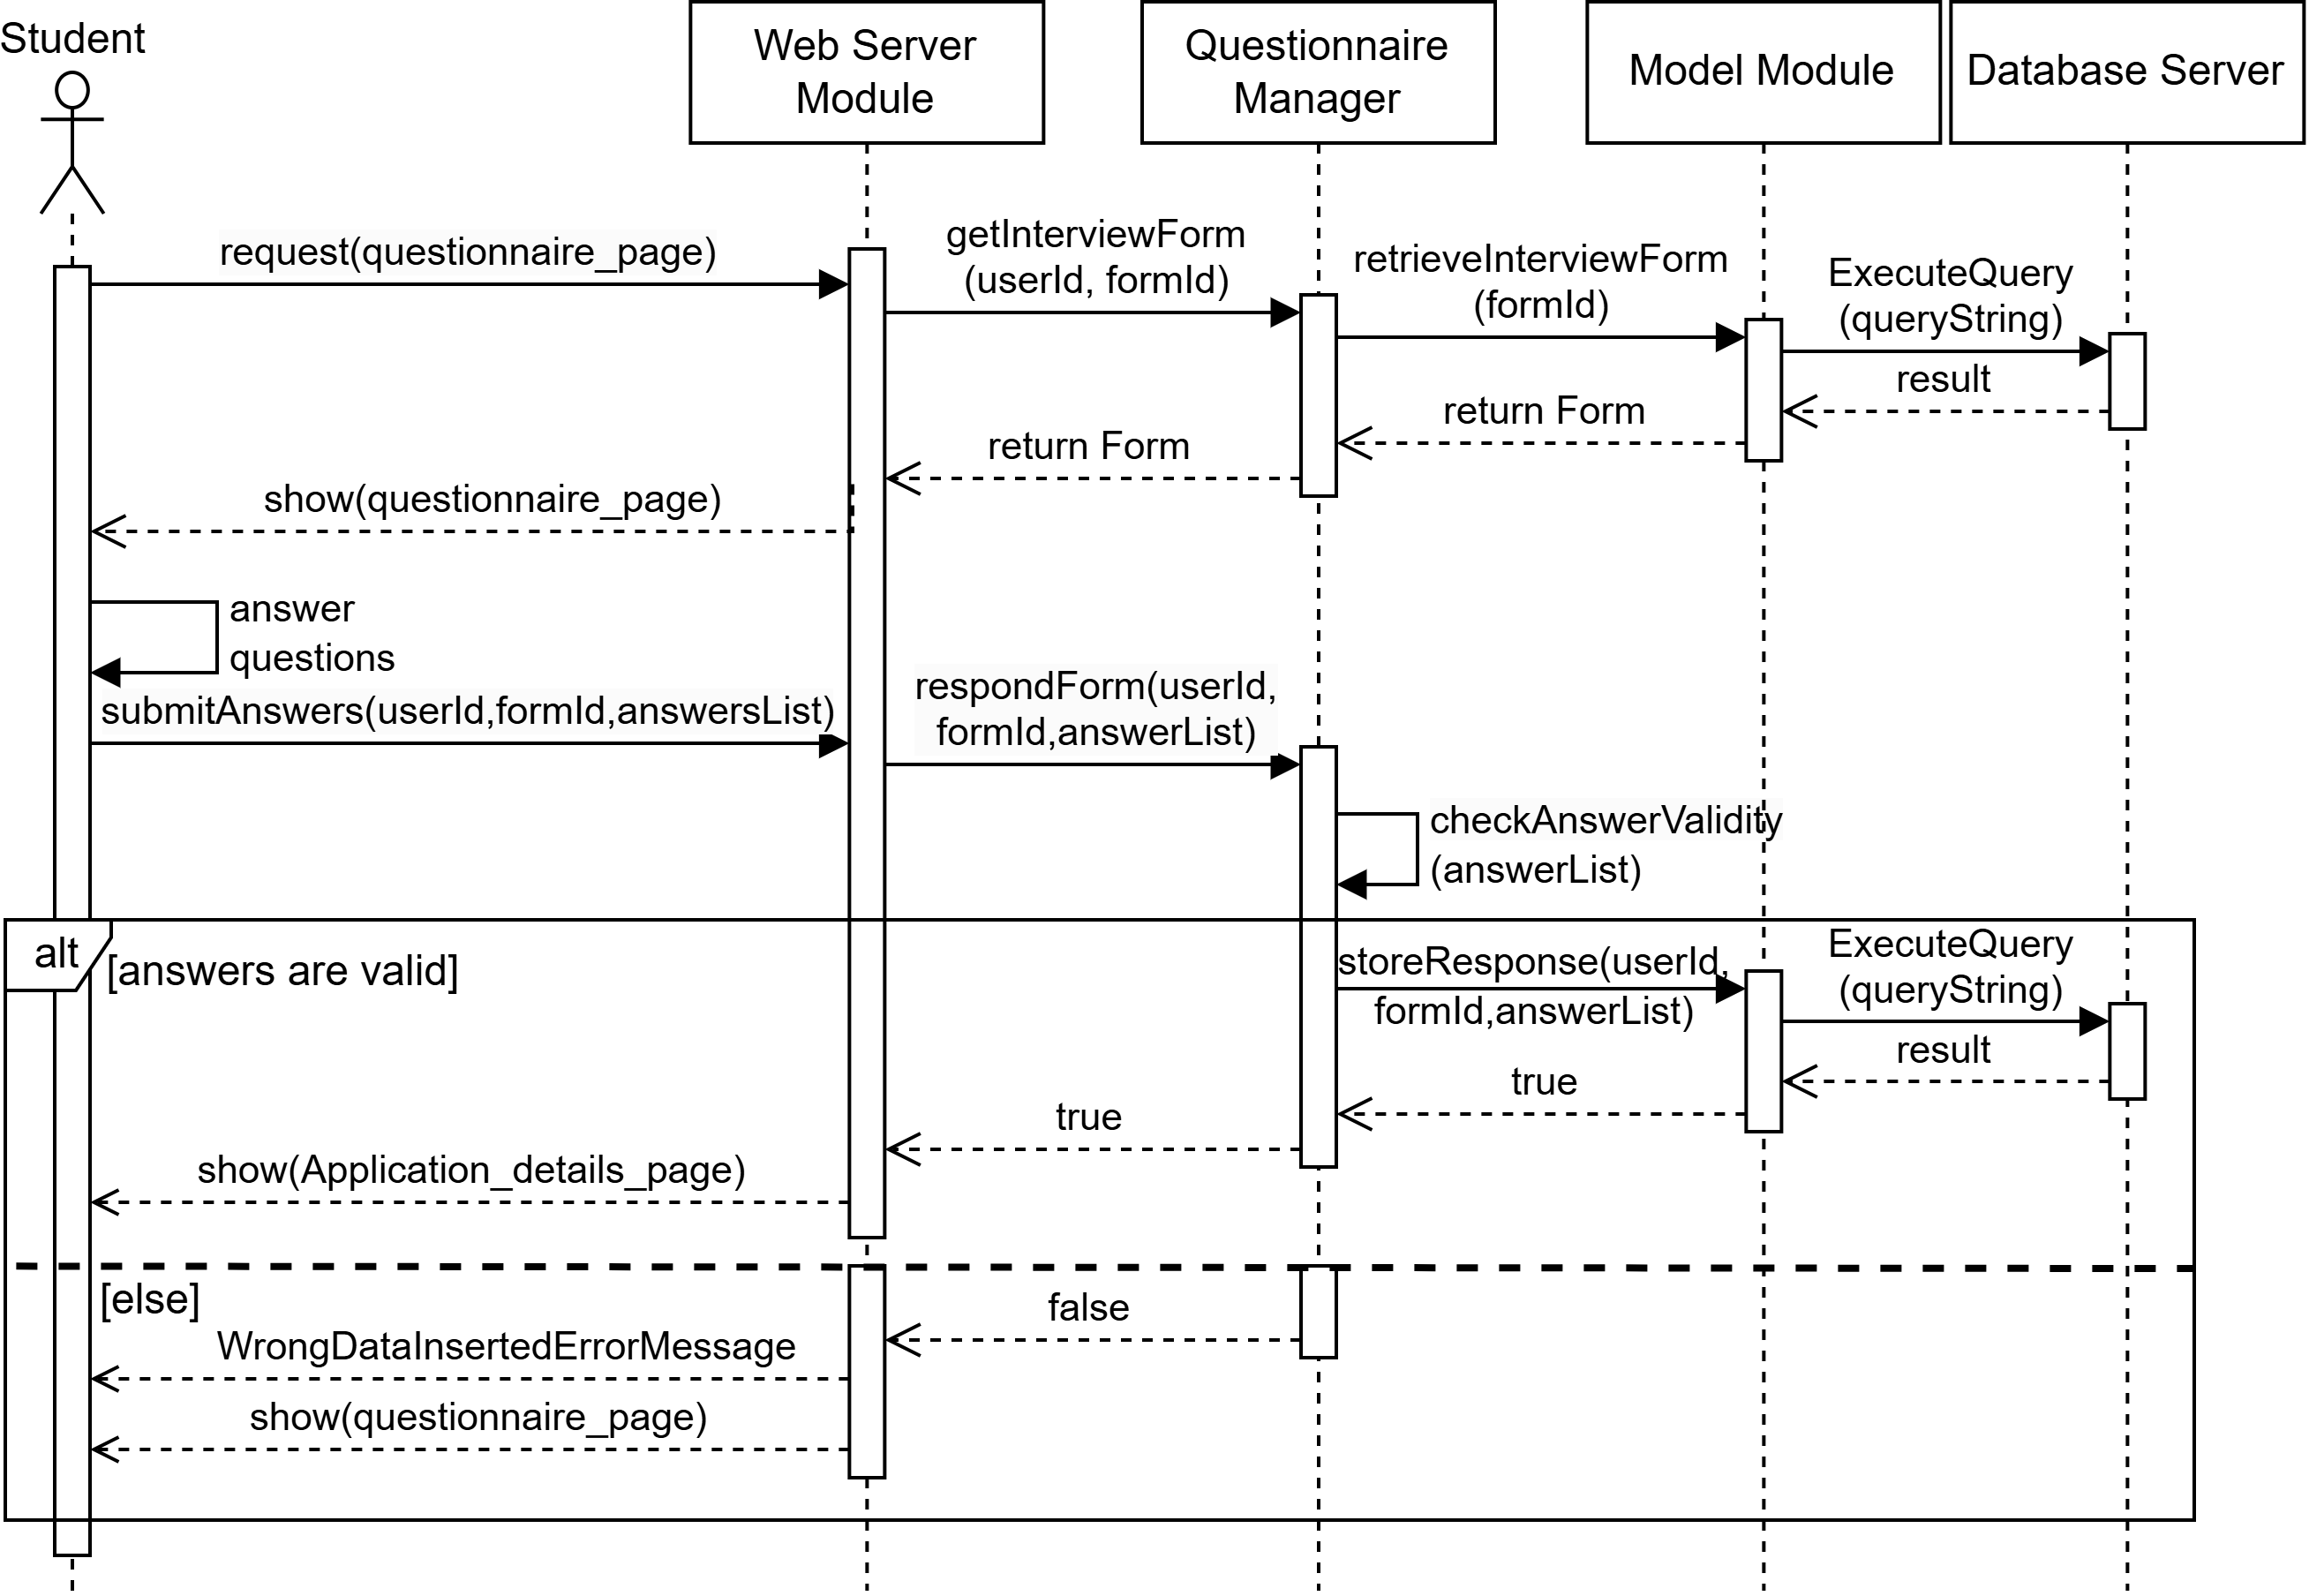
\includegraphics[width=1\textwidth]{Images/Runtime_view/respondQuest_SD.png}
    \caption{Student responds to an interview questionnaire Sequence Diagram}
\end{figure}
% Use Case 10
\begin{figure}[H]
    \centering
    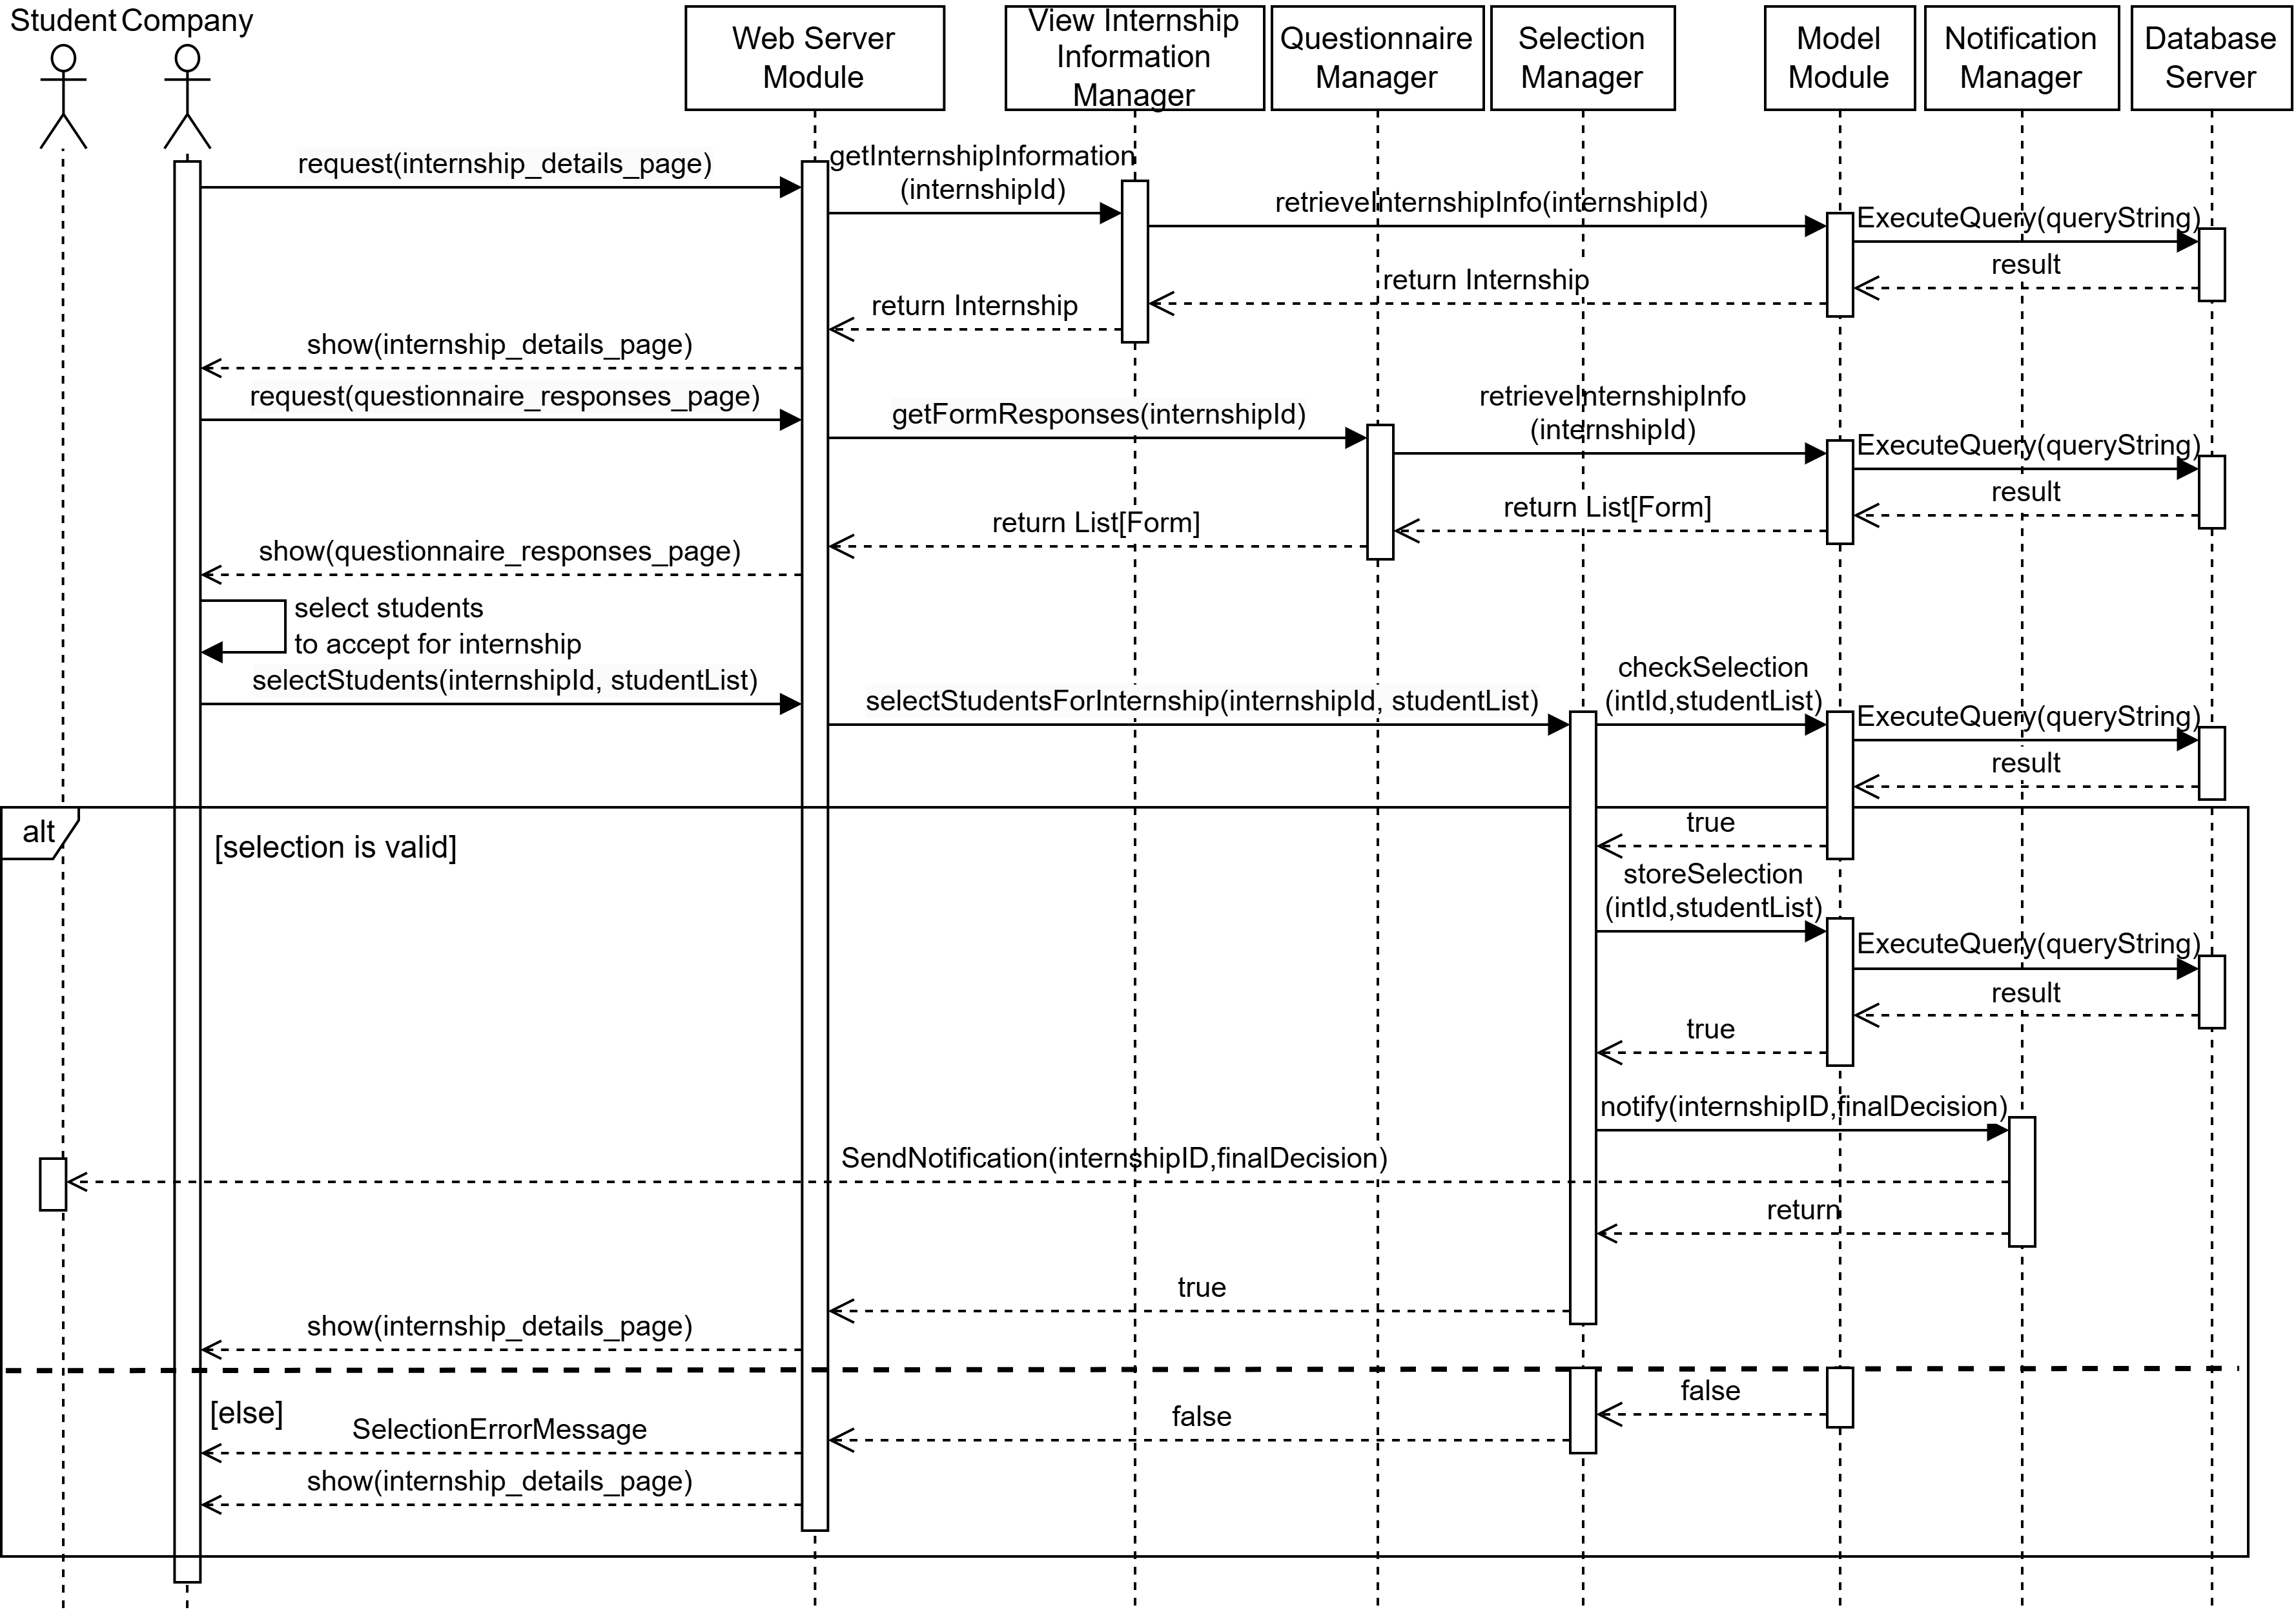
\includegraphics[width=1\textwidth]{Images/Runtime_view/intResults_SD.png}
    \caption{Company sends interview results Sequence Diagram}
\end{figure}
% Use Case 11
\begin{figure}[H]
    \centering
    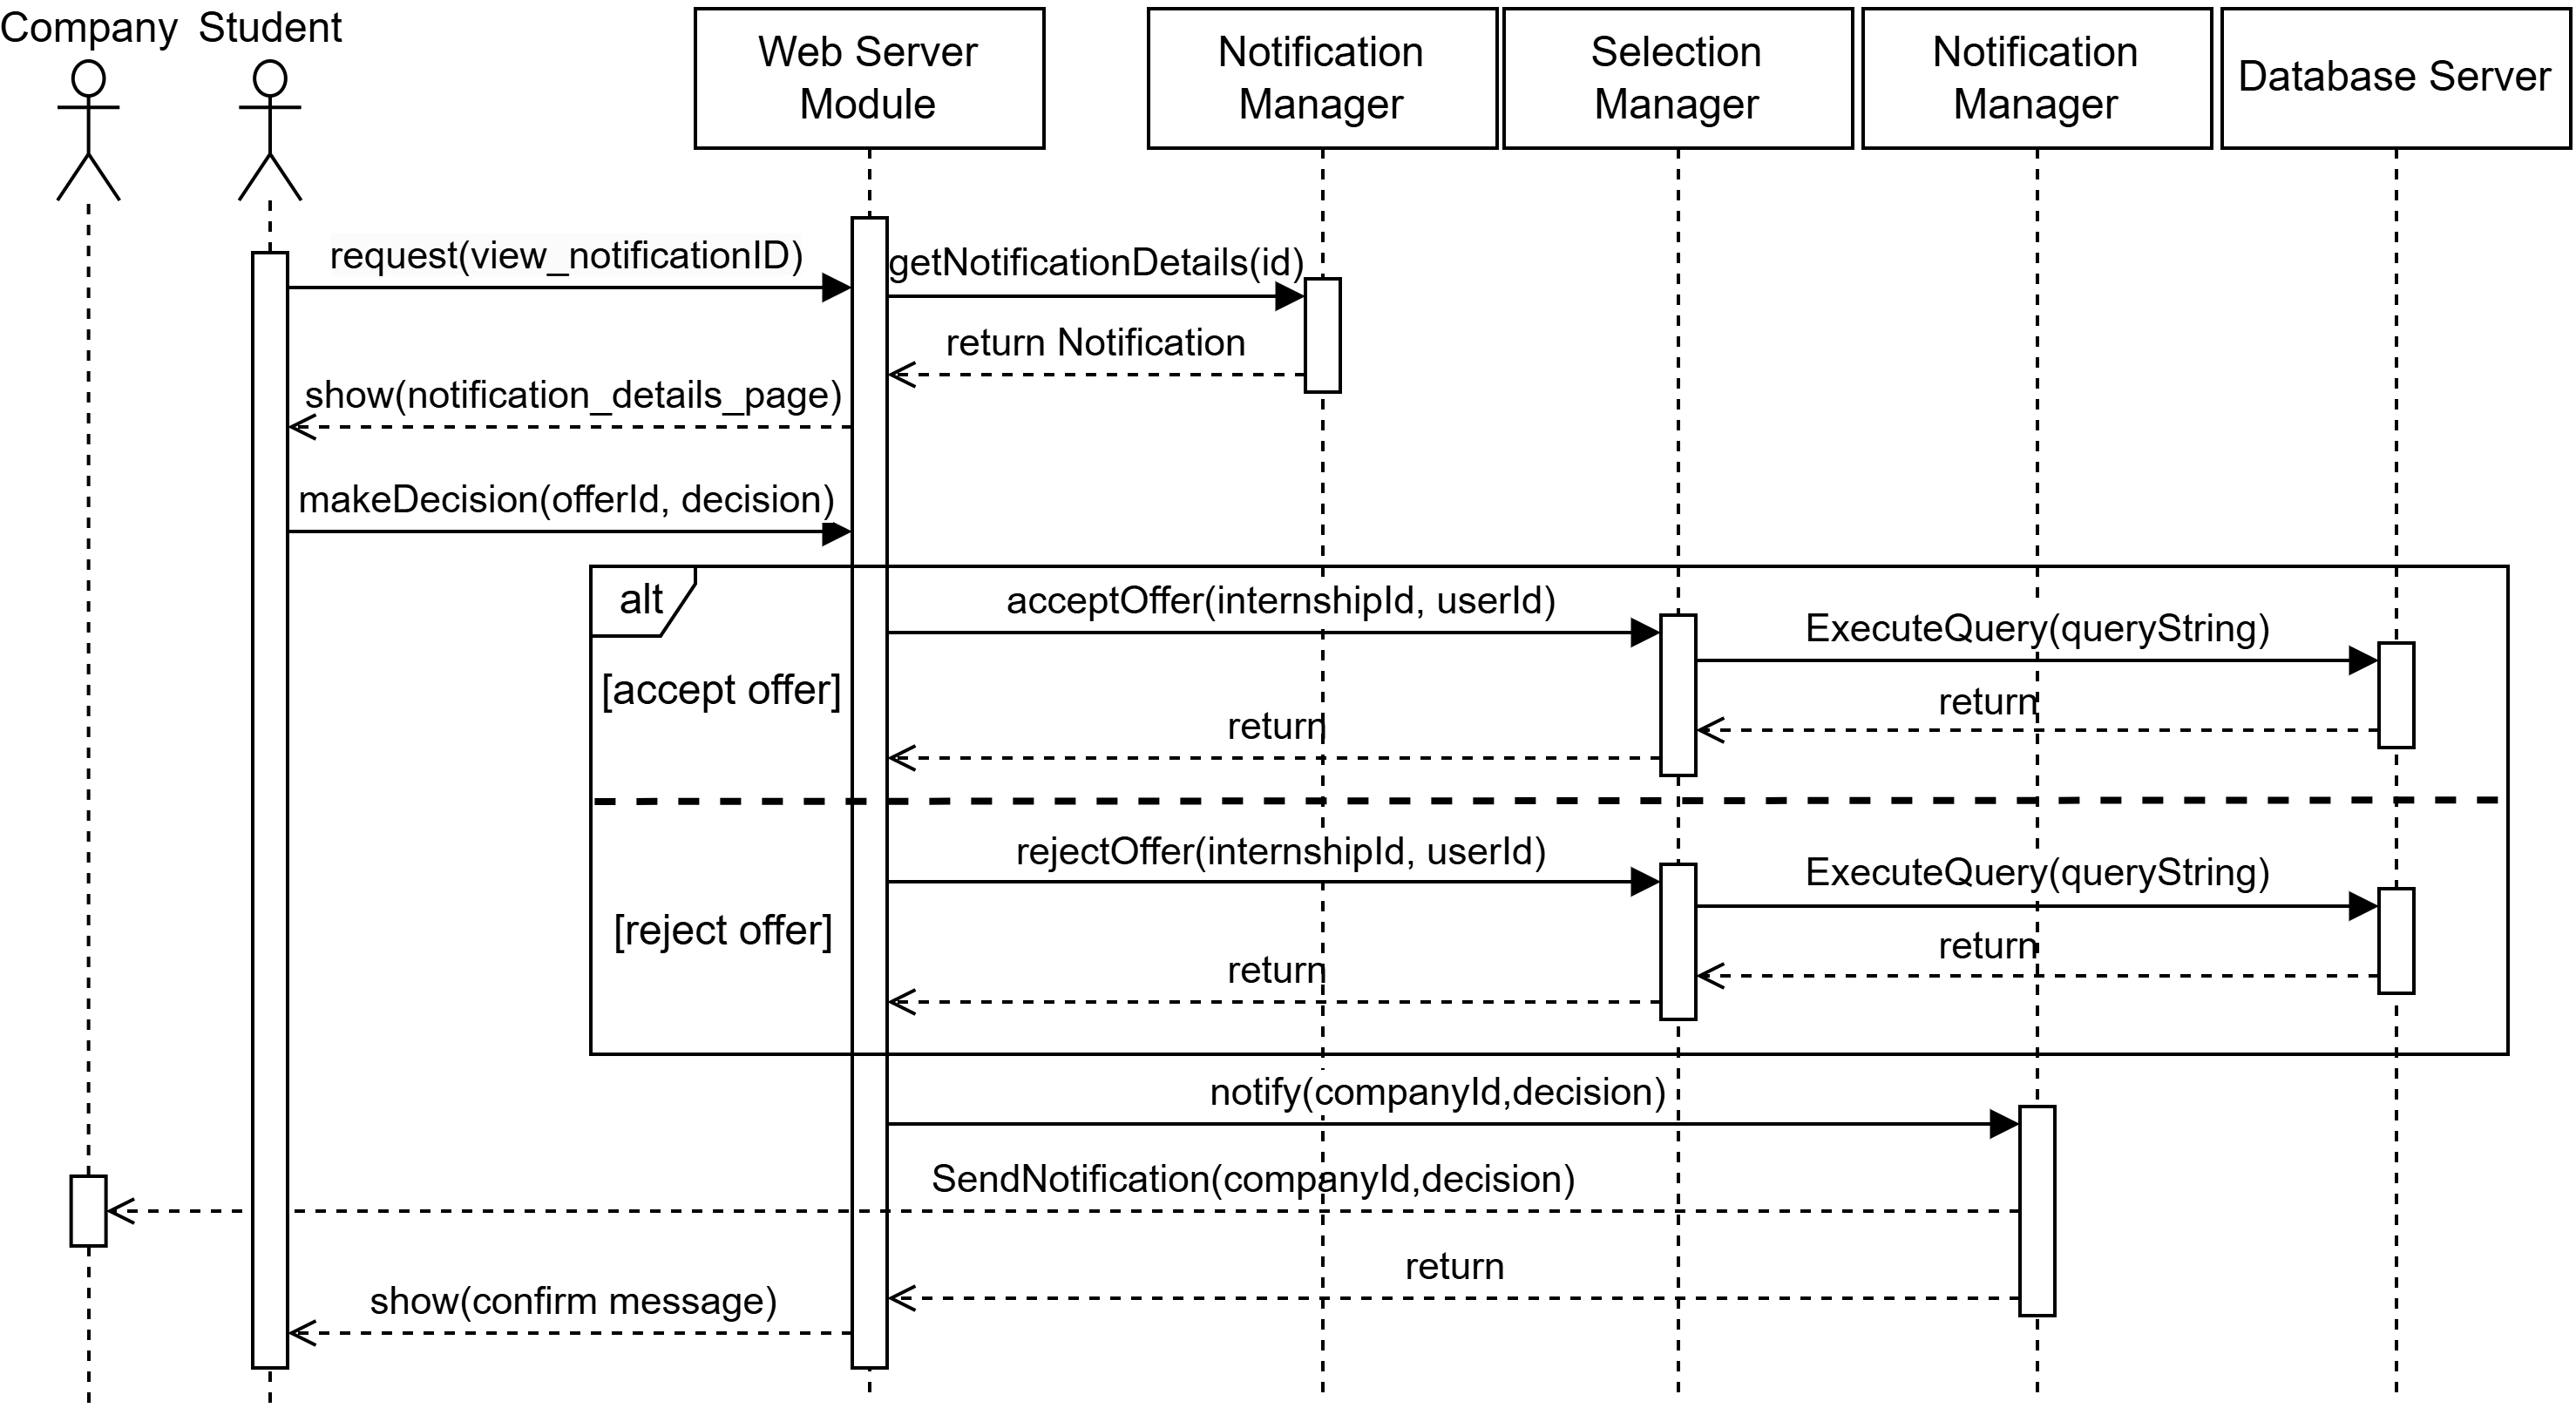
\includegraphics[width=1\textwidth]{Images/Runtime_view/acceptRej_SD.png}
    \caption{Student accepts/rejects an offer Sequence Diagram}
\end{figure}
% Use Case 12
\begin{figure}[H]
    \centering
    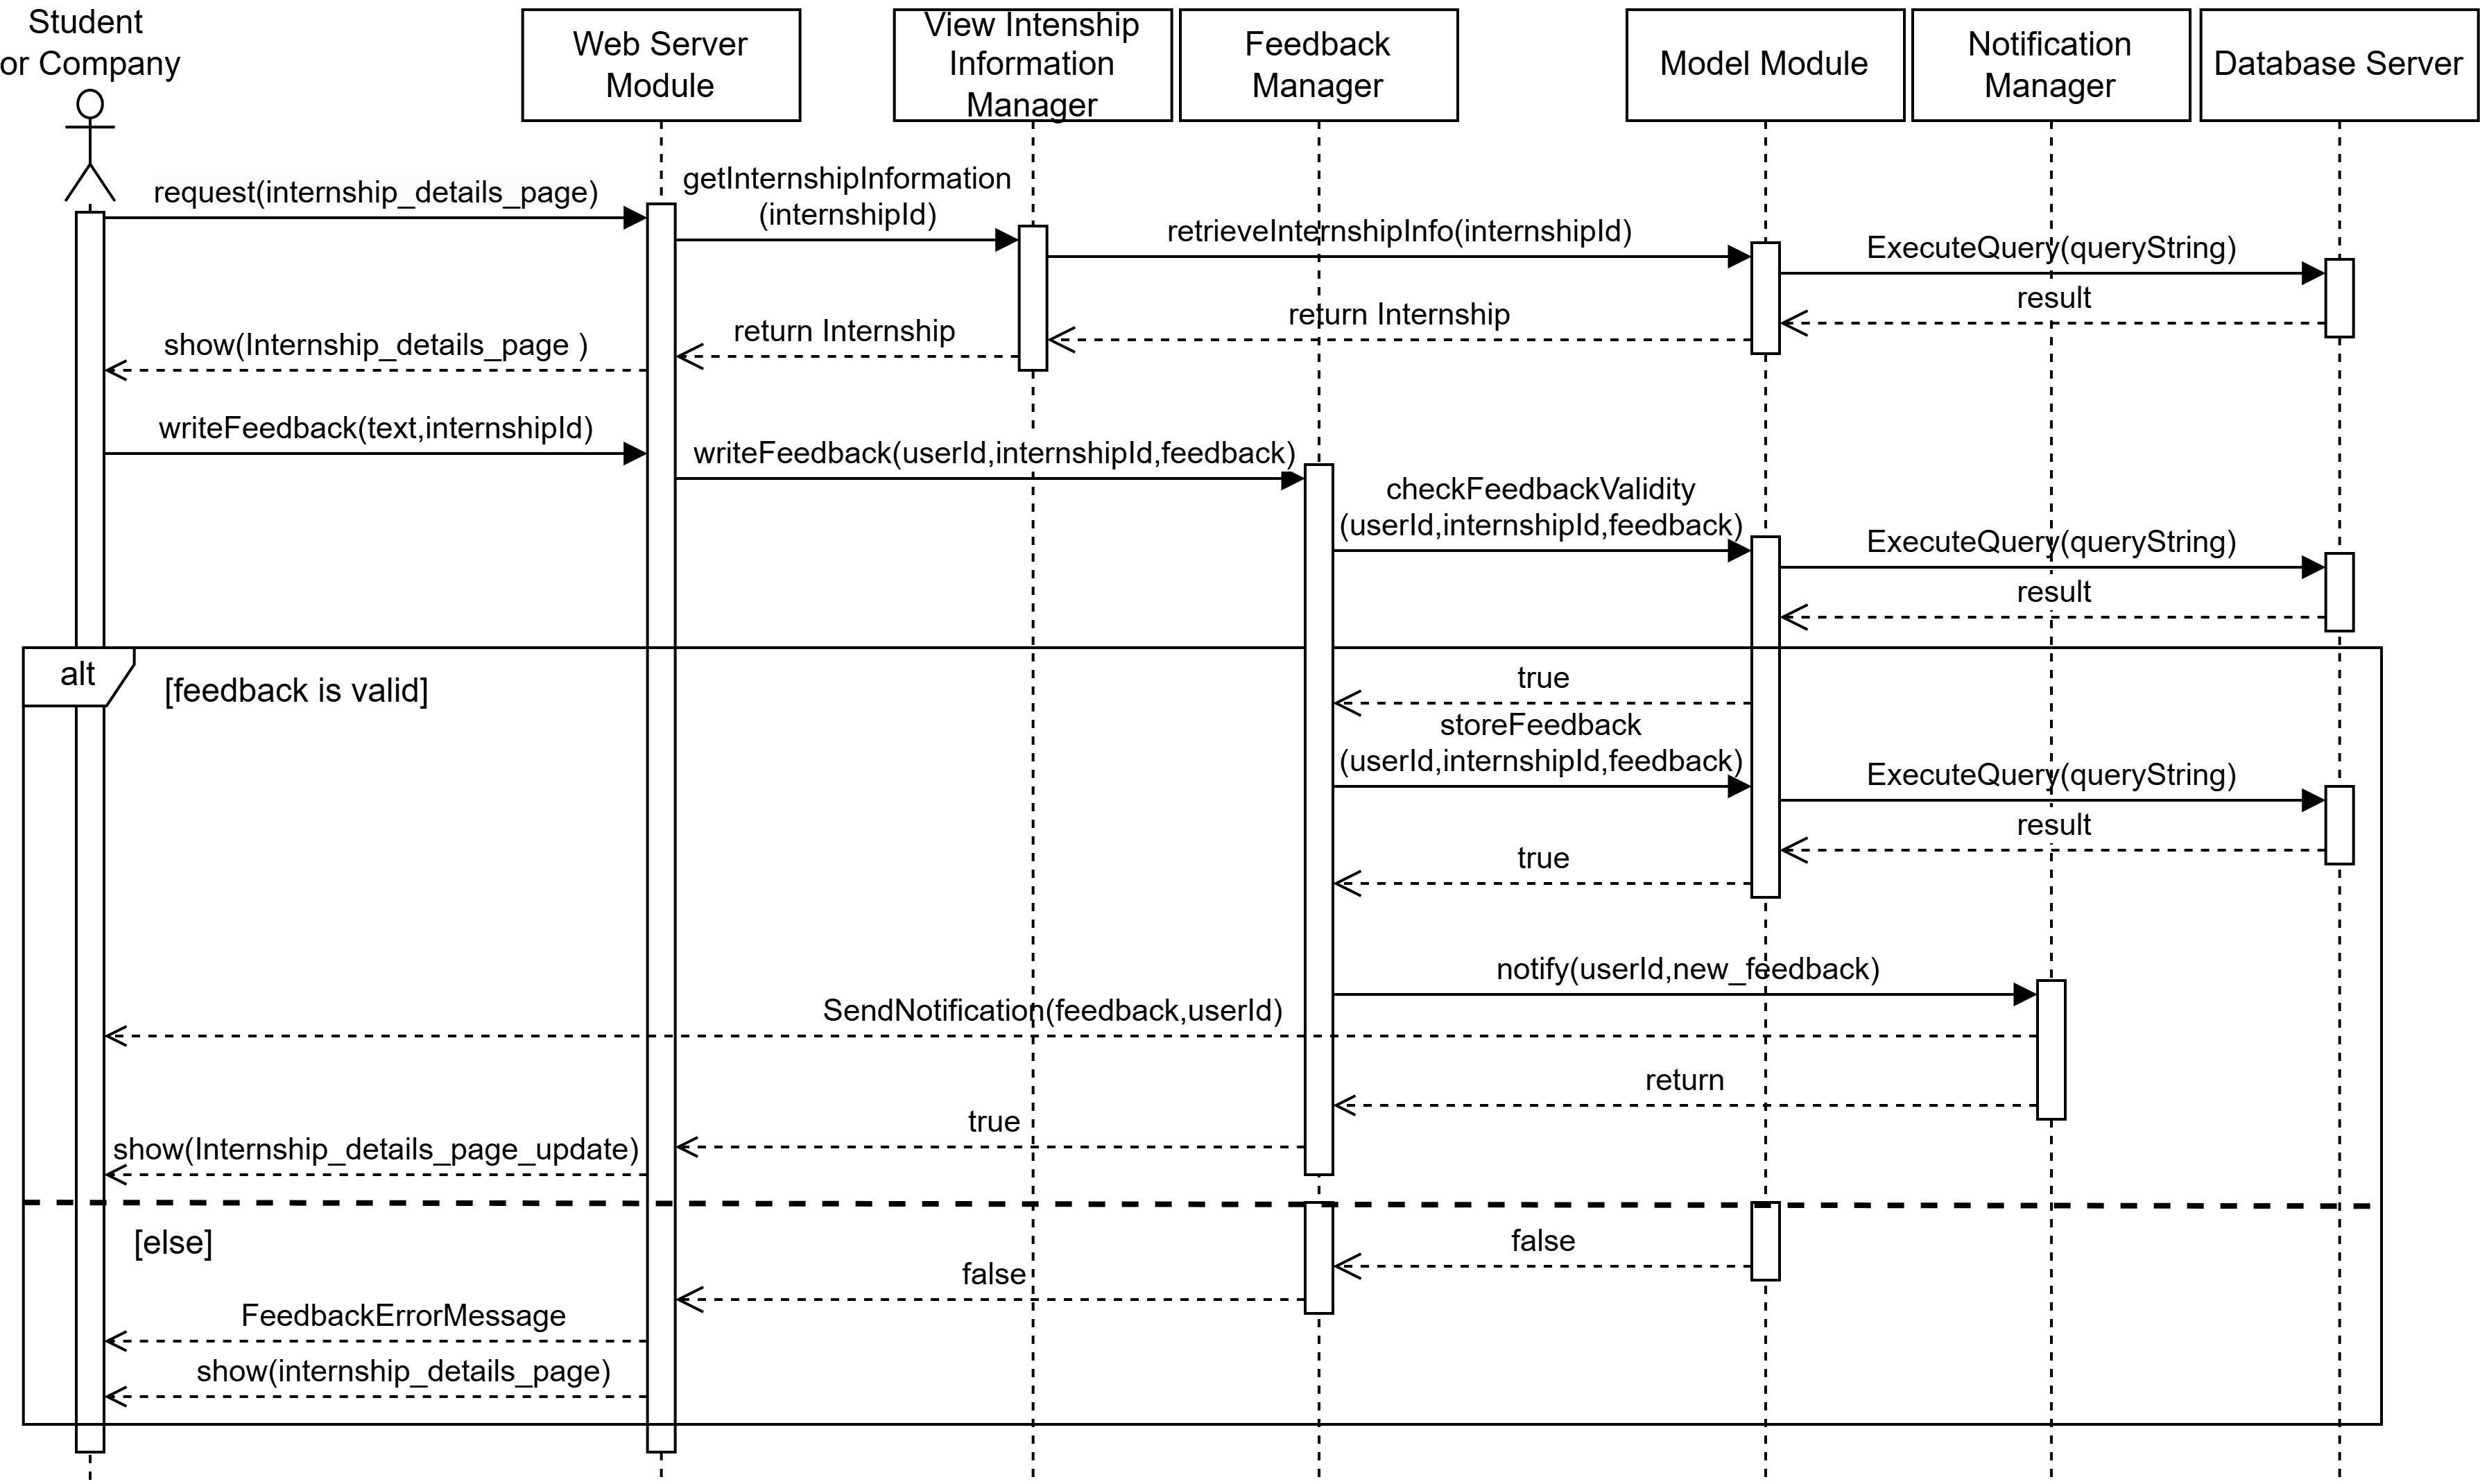
\includegraphics[width=1\textwidth]{Images/Runtime_view/feedback_SD.png}
    \caption{Student or Company writes feedback Sequence Diagram}
\end{figure}
% Use Case 13
\begin{figure}[H]
    \centering
    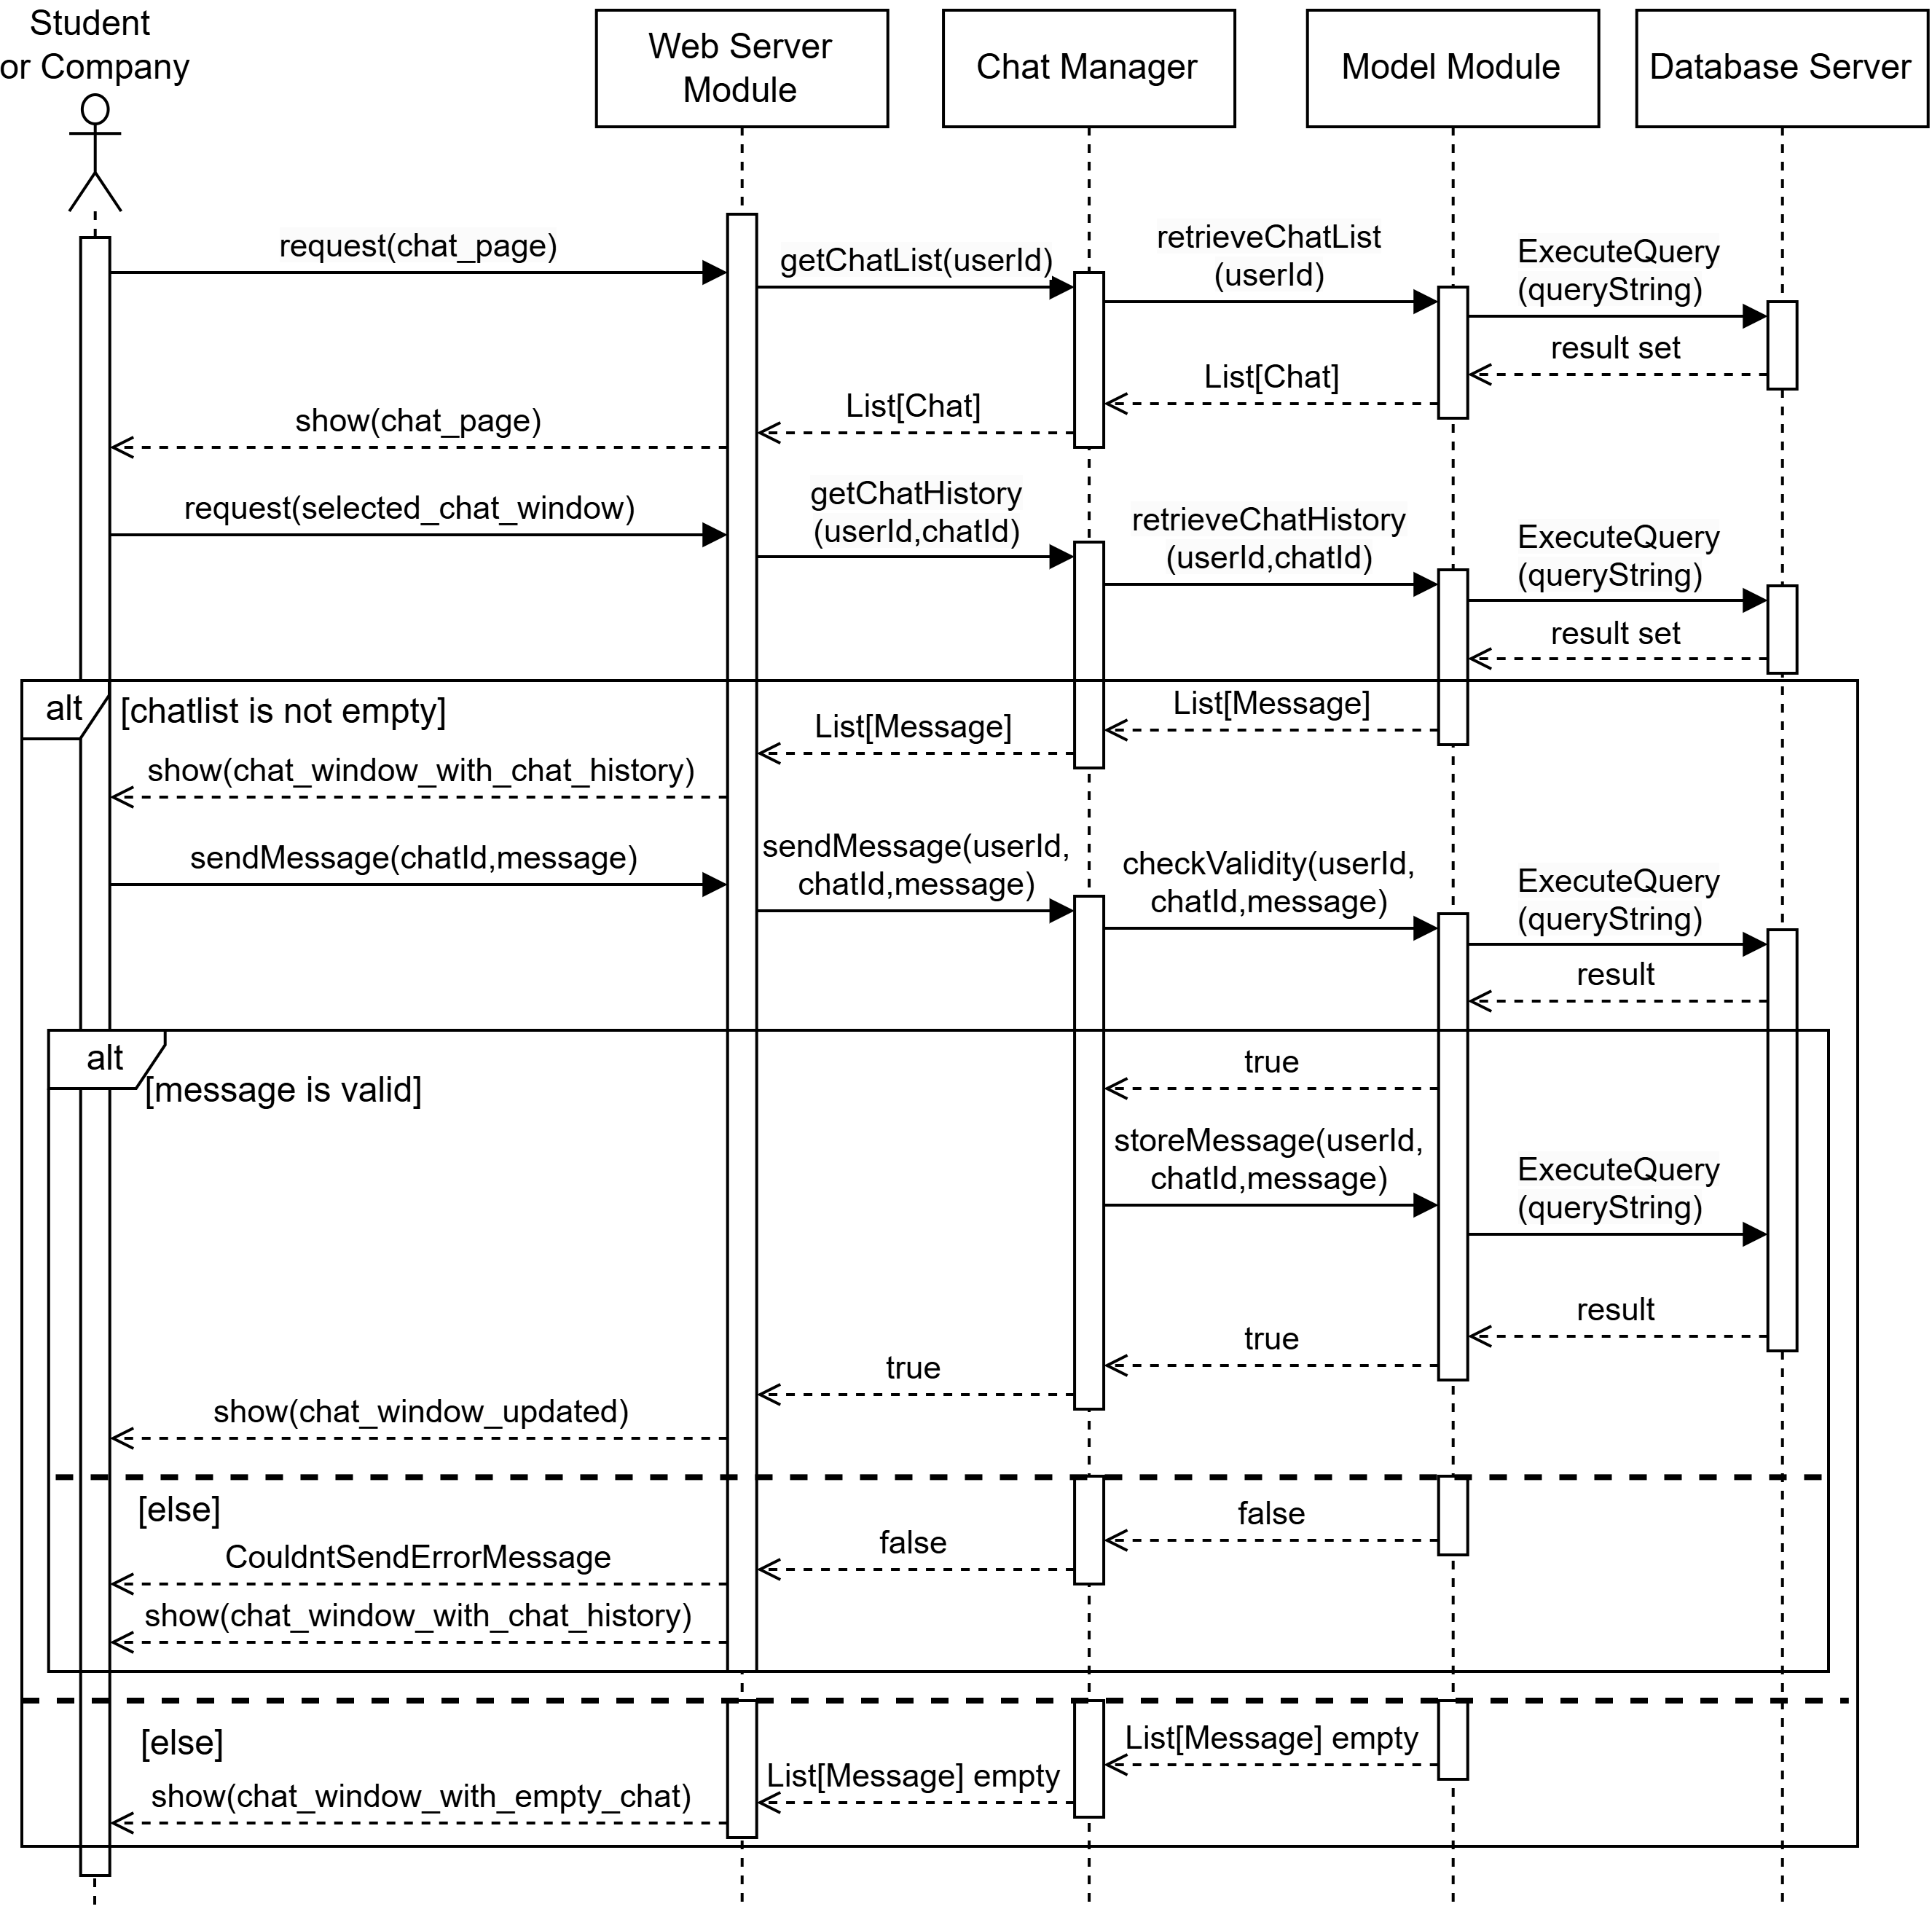
\includegraphics[width=0.86\textwidth]{Images/Runtime_view/chatting_SD.png}
    \caption{Student or Company chats with each other Sequence Diagram}
\end{figure}
% Use Case 14
\begin{figure}[H]
    \centering
    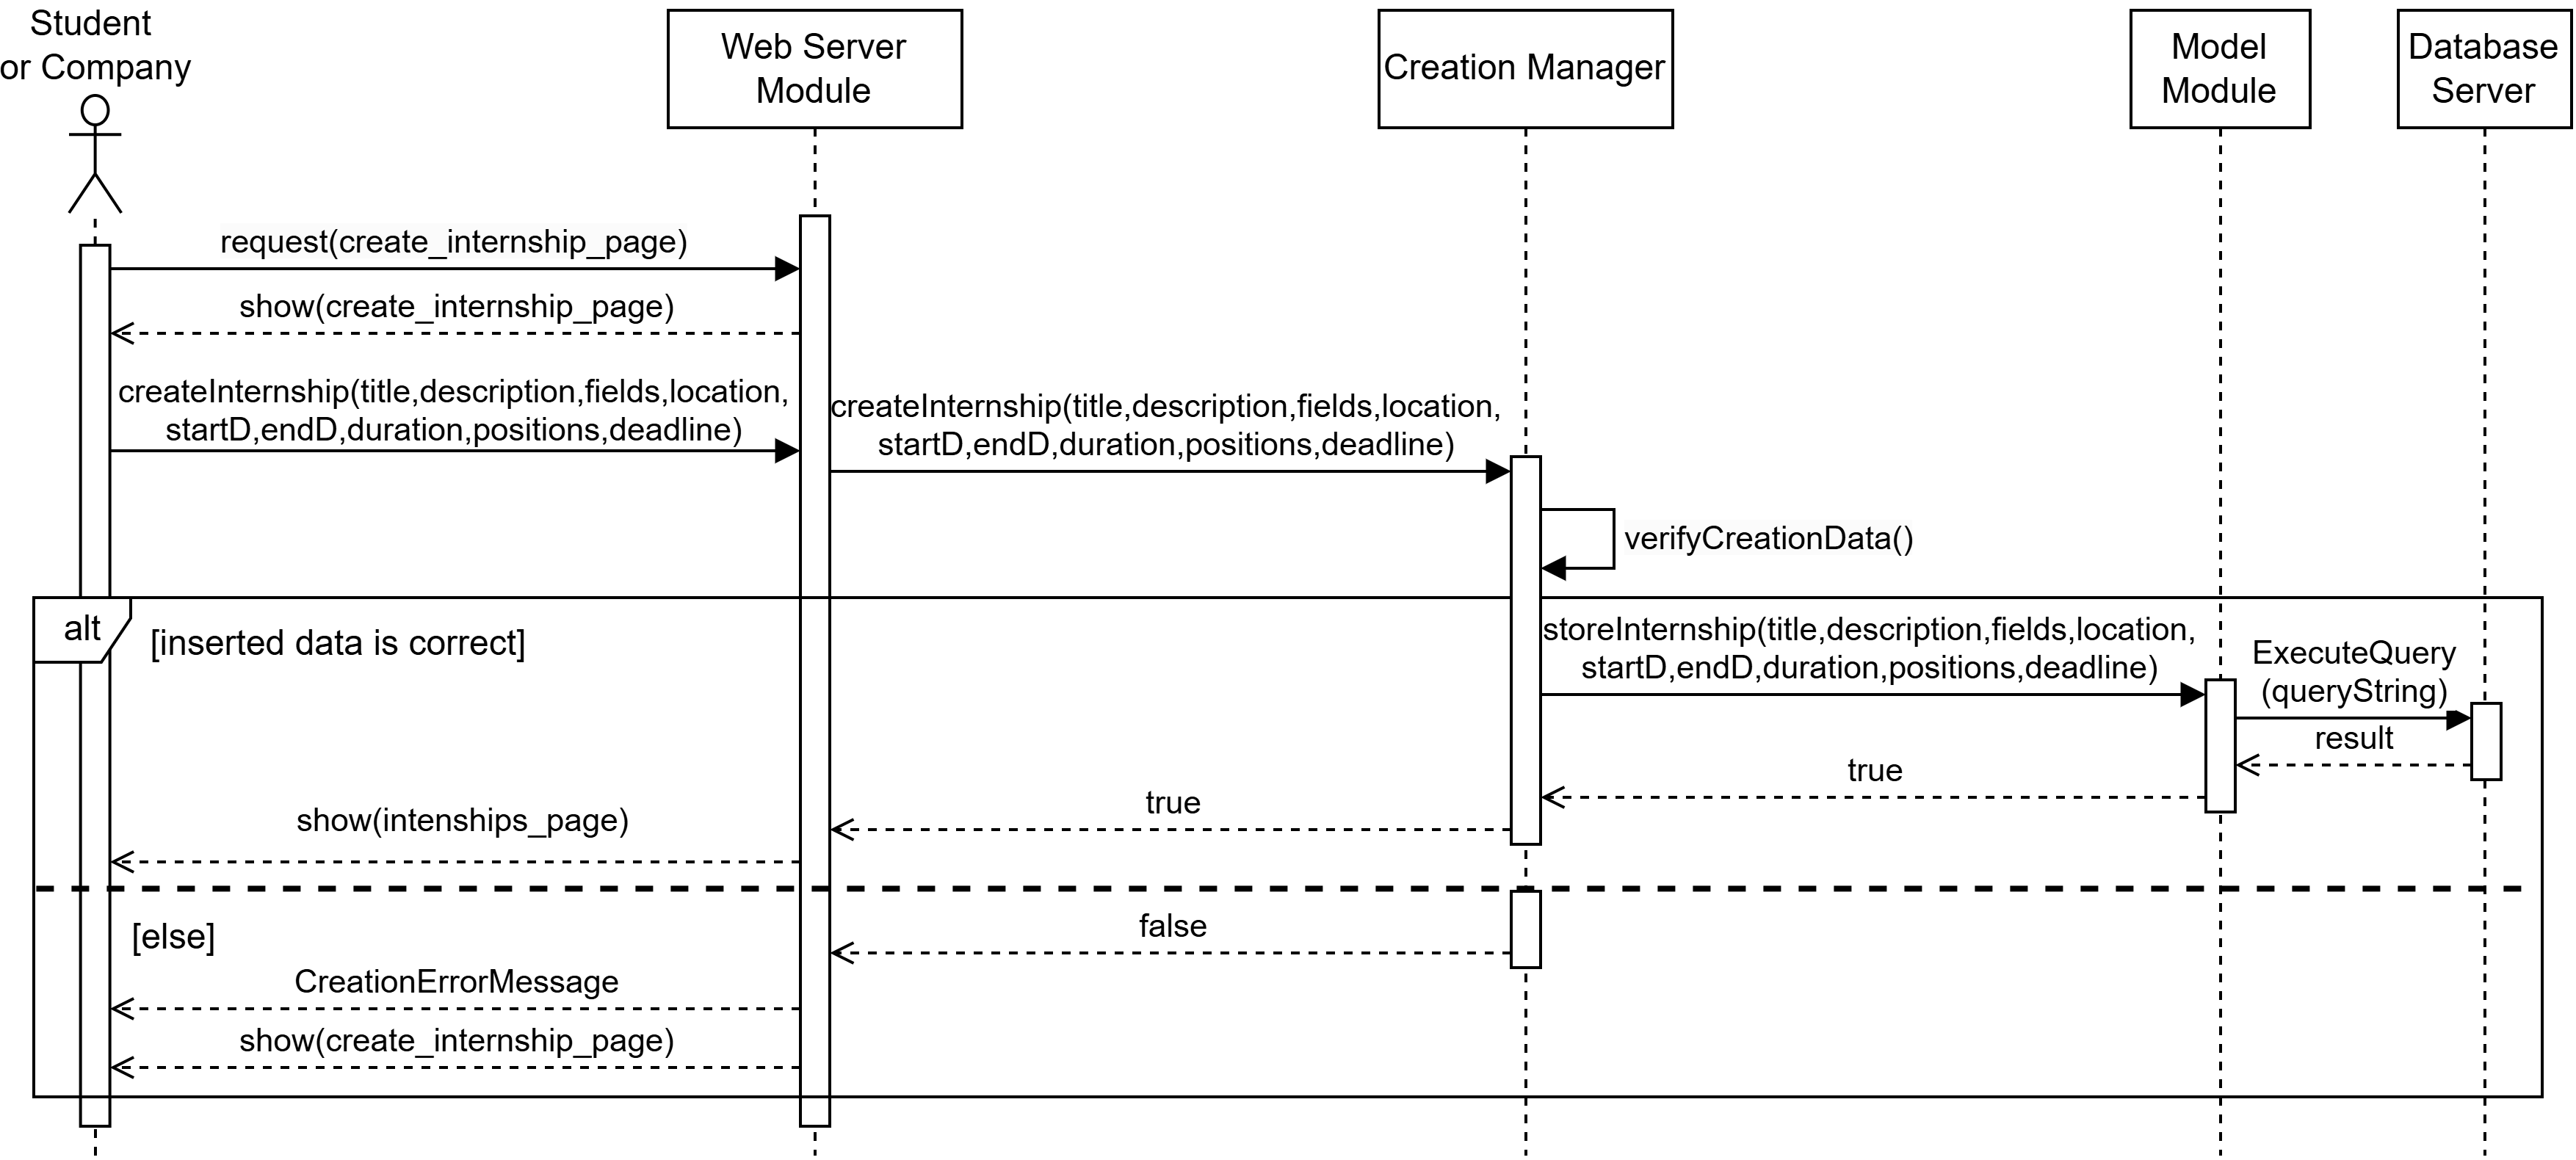
\includegraphics[width=0.94\textwidth]{Images/Runtime_view/createInt_SD.png}
    \caption{Company creates and publishes an internship Sequence Diagram}
\end{figure}
% Use Case 15
\begin{figure}[H]
    \centering
    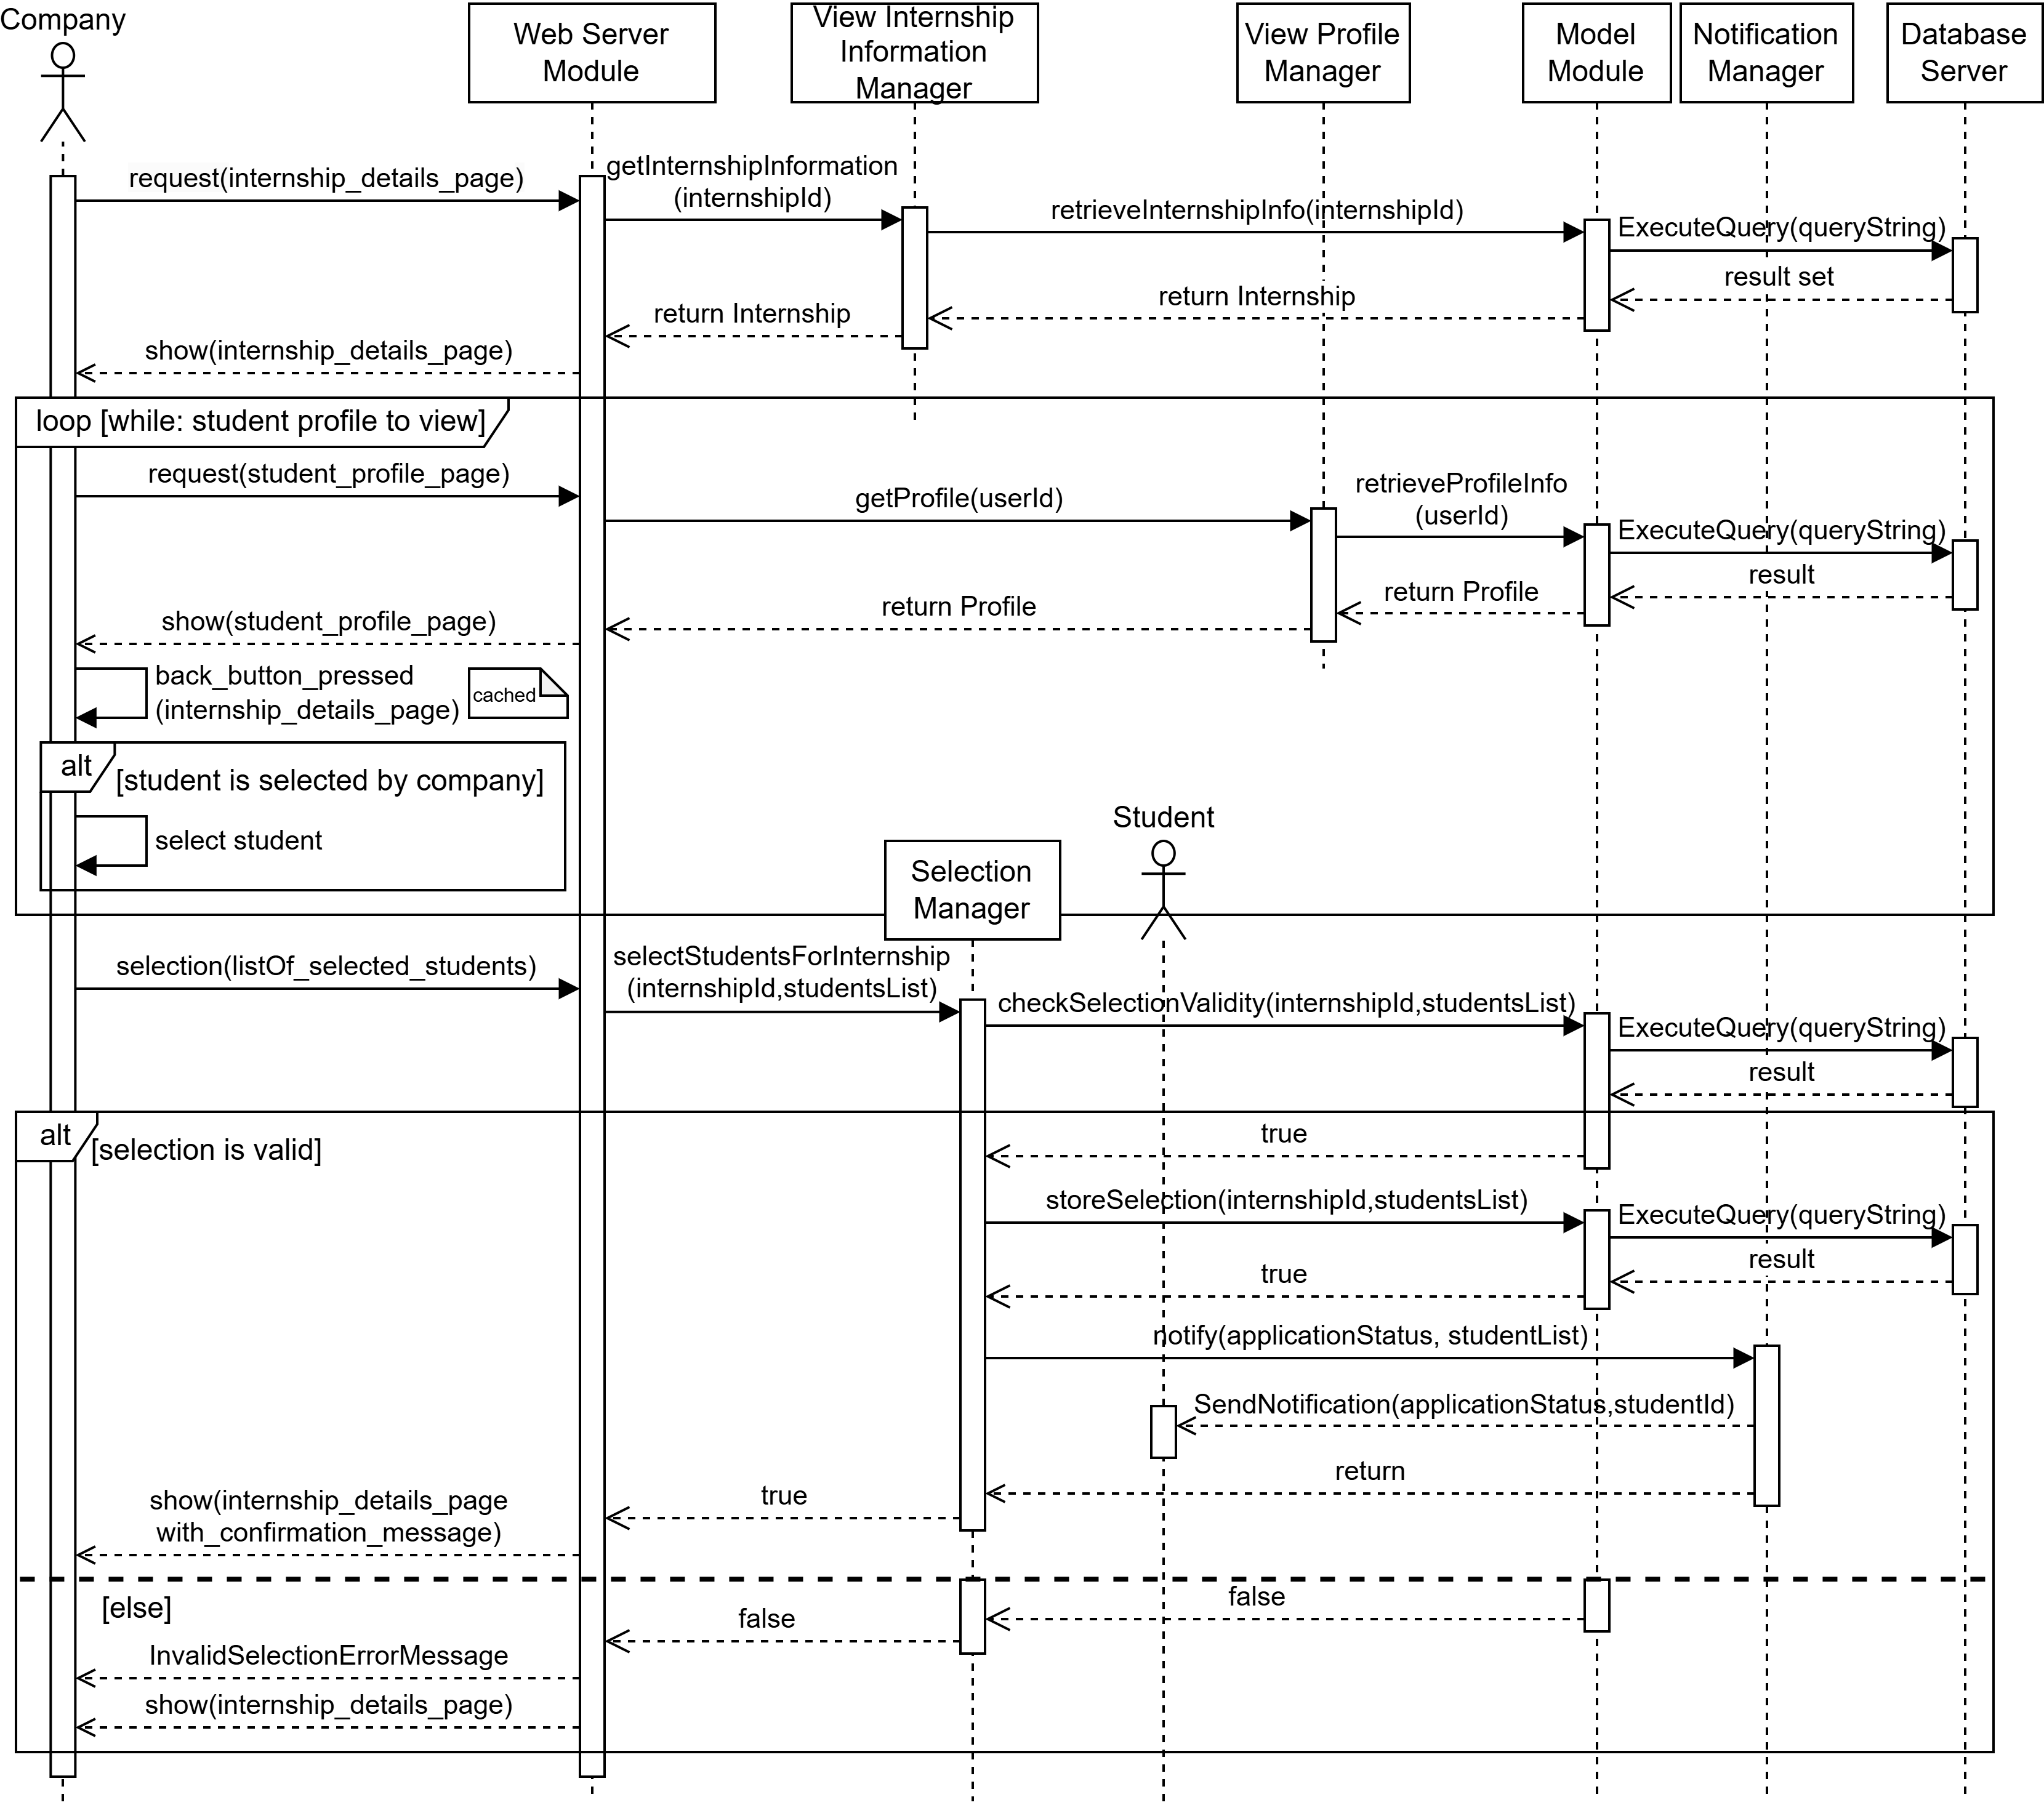
\includegraphics[width=1\textwidth]{Images/Runtime_view/select_SD.png}
    \caption{Company selects candidates Sequence Diagram}
\end{figure}
% Use Case 16
\begin{figure}[H]
    \centering
    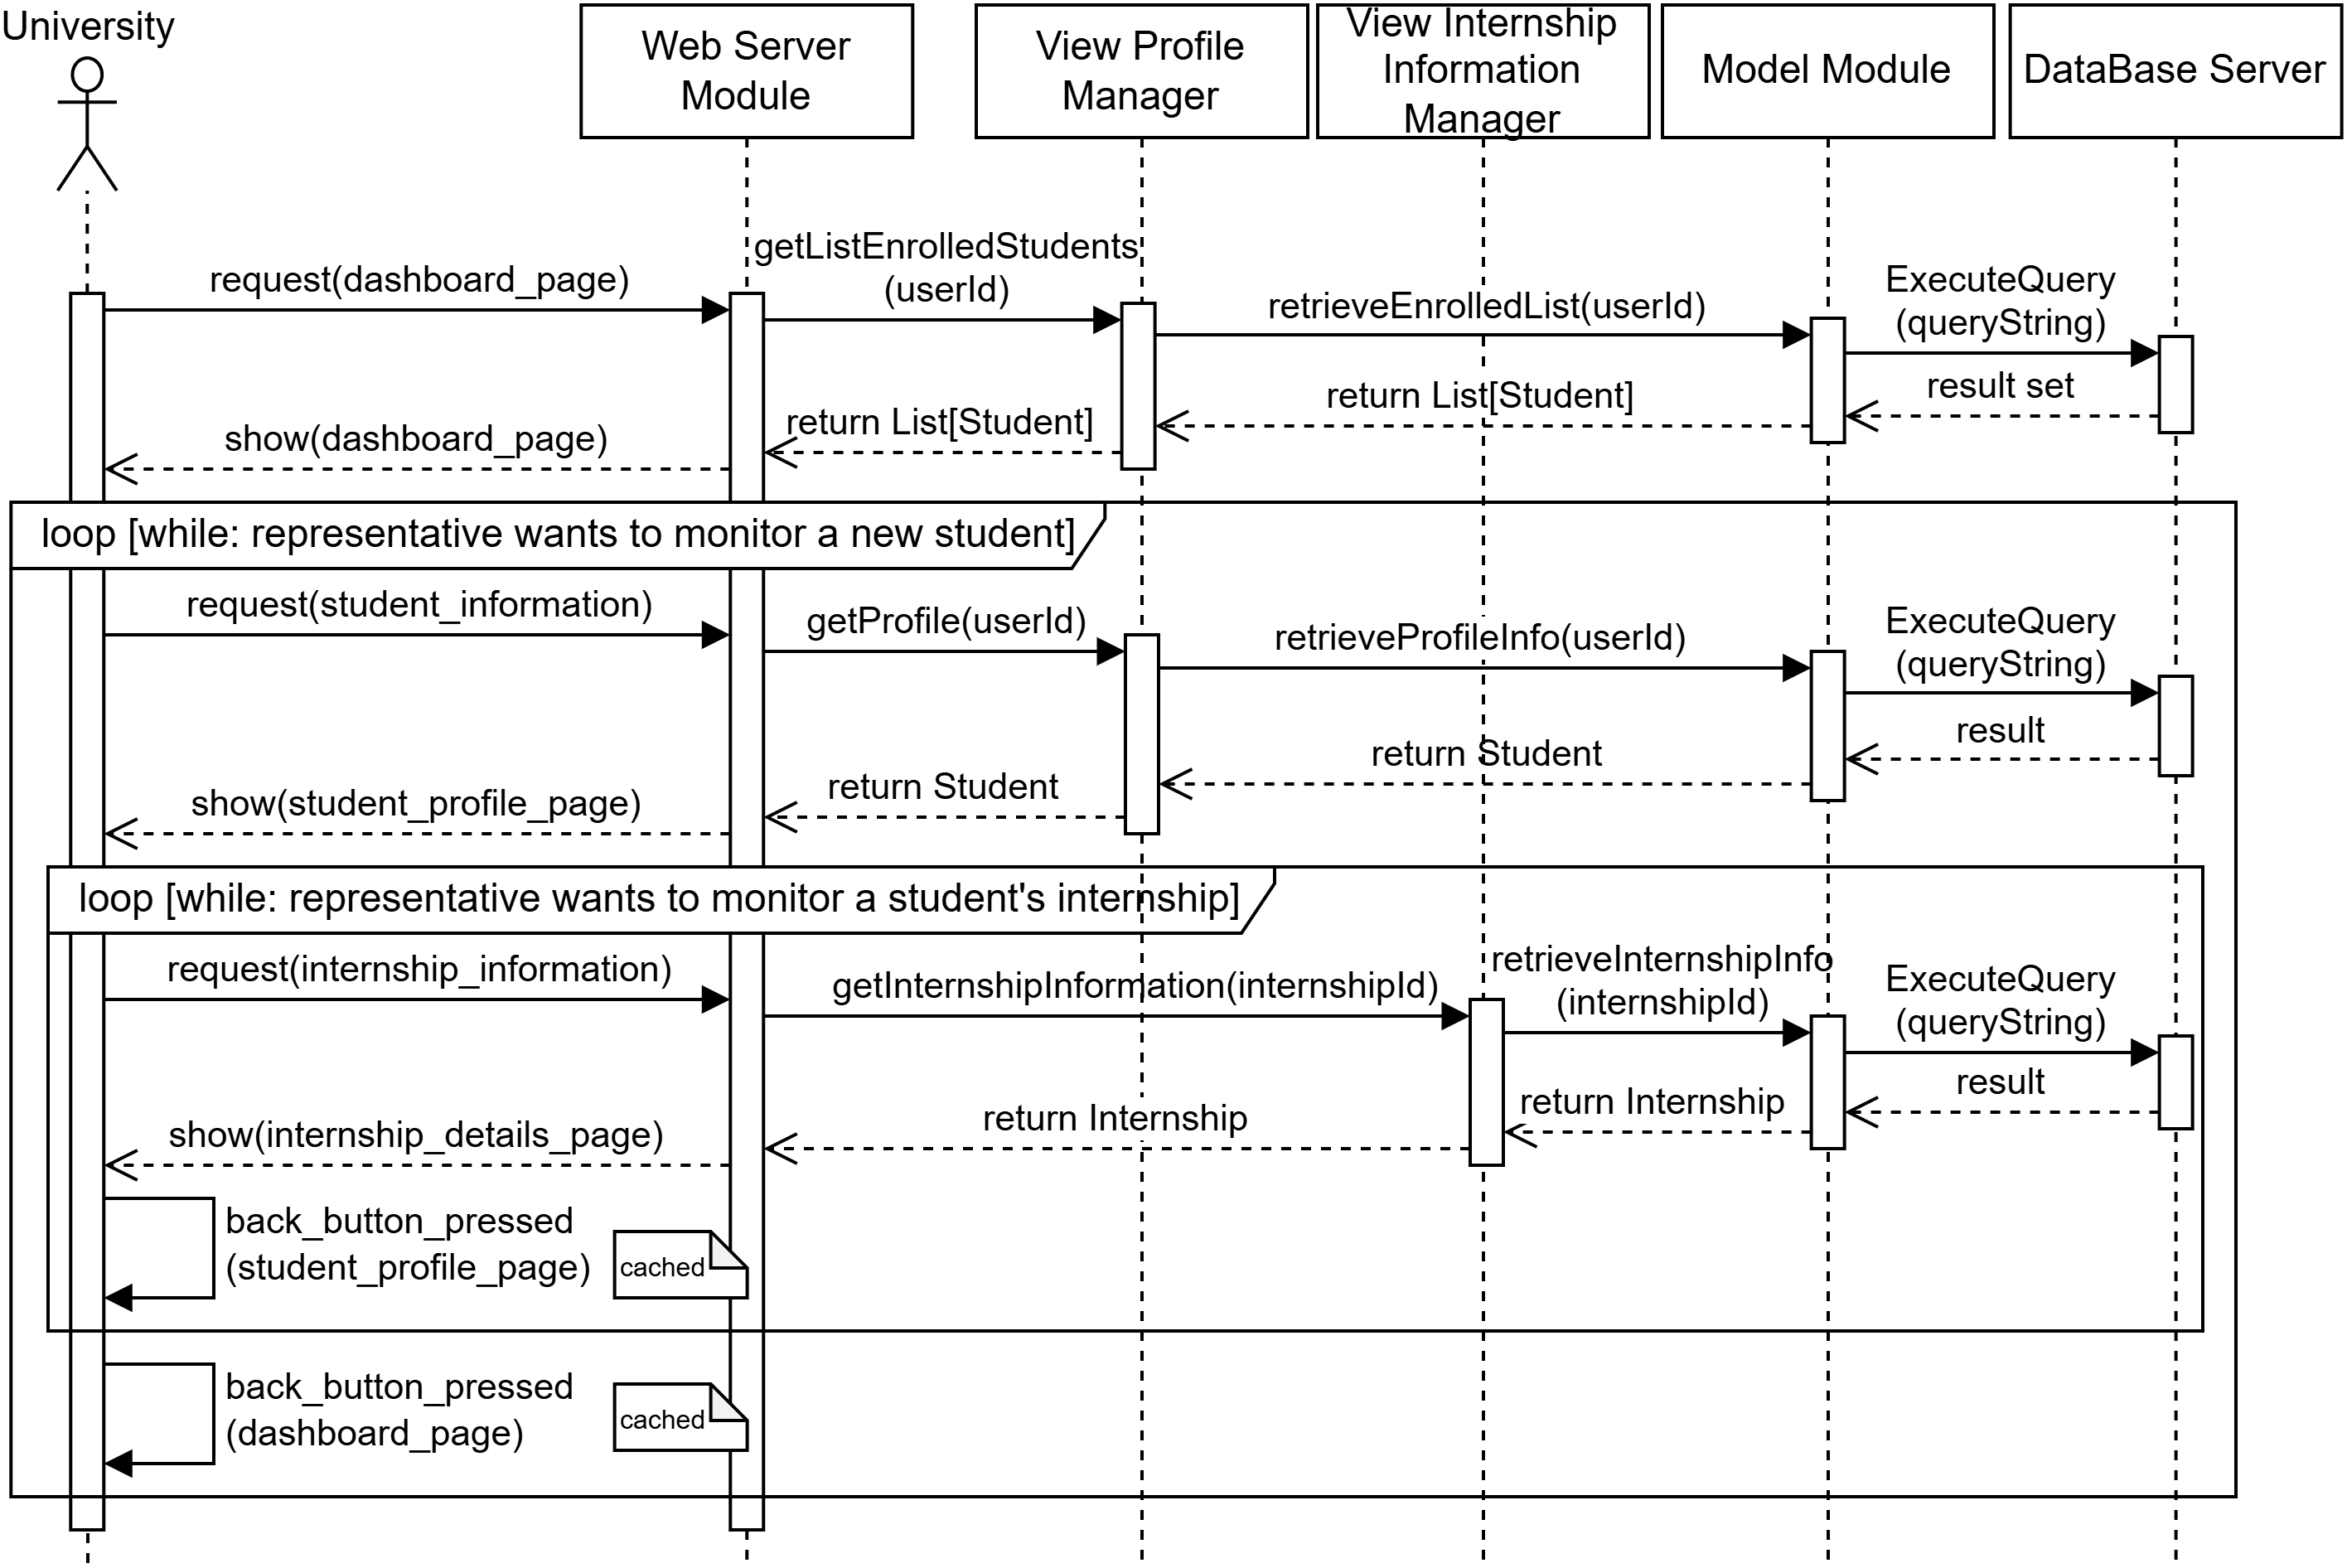
\includegraphics[width=1\textwidth]{Images/Runtime_view/monitor_SD.png}
    \caption{University monitors the internship processes of students Sequence Diagram}
\end{figure}


\section{Selected architectural styles and patterns}\label{sec:selected architectural styles and patterns}
\subsection{Three-Tiered Architecture}\label{subsec:three-tiered architecture}
As described in Section Overview, the Students\&Companies (S\&C) platform is build using a multi-tier architecture. This decision was made with the aim of 
providing a more scalable and flexible system.
The system is divided into three main layers: the presentation layer, the application layer, and the data layer.
Each layer has its own responsibilities and plays a specific role in the system: the presentation layer serves as the front end, accessible through the GUI, 
while the application layer and data layer together form the back end of the system, accessible via API-based methods.
\begin{itemize}
    \item \textbf{Presentation Layer:} The presentation layer is implemented as a generic web application accessible through a web browser.
    It is responsible for managing the presentation logic, including user interaction, the user interface, and rendering information.
    This layer serves as the front end of the system, the only part that the user can access directly.
    \item \textbf{Application Layer:} The application layer is implemented as a set of RESTful web services.
    It is responsible for managing the functional logic of the system, controlling communication between the presentation layer and the data layer.
    This layer allows the system to react to user input and generate appropriate responses accordingly.
    It includes the Application Server and is also used to interact with third-party services.
    \item \textbf{Data Layer:} The data layer is responsible for managing the data storage and access within the system.
    All operations that require data manipulation must be performed through interactions with the data layer.
    The platform uses a Relational Database Management System (RDBMS), making the data accessible through SQL queries.
\end{itemize}
\subsection{RESTful API}\label{subsec:restful api}
The Representational State Transfer (REST) style is designed to be stateless, enabling more efficient and seamless communication between the client and the 
server. It uses standard HTTP methods (GET, POST, PUT, DELETE) to perform operations on resources.
The decision to incorporate RESTful APIs into the architecture provides advantages in terms of performance, modifiability, and simplicity by defining conventions 
for interacting with resources in resource-oriented manner.
\subsection{Model-View-Controller (MVC) Pattern}\label{subsec:model-view-controller pattern}
One of the most recommended design patterns for the Three-Tier Architecture is the Model-View-Controller (MVC) pattern. It separates the application into three 
components: the model, the view, and the controller, minimizing interdependencies between the components and improving the maintainability, manageability, and 
scalability of the system. Each component can be developed, tested, and maintained independently.
\begin{itemize}
\item \textbf{Model:} Contains the state and application logic and is independent of the other components.
\item \textbf{View:} Represents the visual presentation logic of the Model and is responsible for displaying data to the user.
\item \textbf{Controller:} Acts as an intermediary between the Model and the View. It receives user input forwarded by the View, then processes operations and 
updates the Model and the View accordingly.
\end{itemize}

\section{Other design decisions}\label{sec:other design decisions}
\begin{itemize}
    \item \textbf{Design patterns related to the behavioral aspects:} Observer Pattern and State Pattern.
    \item \textbf{Design decisions related to the system's requirements:} Some design decisions are already described in the RASD, such as reliability, 
    availability, scalability, security, maintainability, and portability. 
    The following sections revisit availability, scalability, and security to emphasize their importance in the system.
\end{itemize}
\subsection{Observer Pattern}\label{subsec:observer pattern}
The Observer pattern is particularly useful when multiple objects need to be notified about a change in the state of another object. In the context of the 
S\&C platform, a large number of functionalities require the participation of multiple objects, such as notifying users about the results of an interview or 
updates on the status of an application.
\subsection{State Pattern}\label{subsec:state pattern}
The State pattern is recommended to efficiently manage operations across different states and handle transitions between them, as it allows objects to change 
their behavior when their internal state changes. In the context of the S\&C platform, the State pattern can be used to manage the lifecycle of an application 
for a internship position.

\subsection{Availability}\label{subsec:availability}
The system is designed to be highly available, ensuring that users can access the platform at any time, as described in the RASD, with at least 99.8 percent 
uptime. To achieve this, critical components should be replicated across multiple servers to provide redundancy and fault tolerance in case of failure. Load 
balancing is correctly configured to distribute incoming traffic, preventing overload on any single server. Continuous monitoring of the system's performance 
allows for the detection and resolution of any issues that may arise in real-time.
\subsection{Scalability}\label{subsec:scalability}
The platform is designed to handle increased user loads in the future by scaling individual layers independently, thanks to the architectural styles and patterns 
mentioned earlier. As described in the RASD, the system can be scaled horizontally by adding more servers or vertically by increasing the resources of existing 
servers, without affecting performance. This scalability is essential, especially as the number of users grows, leading to a higher volume of application 
requests over time.
\subsection{Security}\label{subsec:security}
The system is designed to ensure the privacy and security of user data both during transmission over the network and while stored in the database. This includes 
the use of authentication and authorization mechanisms to ensure that only authorized users can access the system, reducing the risk of unauthorized access. 
Additionally, a firewall and Intrusion Detection System (IDS) are set up in the network to protect the system from external threats and attacks. Protocols like 
HTTPS are used to encrypt communication between the client and server, and other encryption algorithms are employed to protect sensitive data stored in the 
database, such as user passwords.


\clearpage
\chapter{User Interface Design}\label{sect:user interface design}
\section{User Interface Design}
In this section, the user interface design will be presented using mockups within the short description.
The design focuses on optimizing the user experience and ensuring that the user can easily navigate on the website to perform the desired actions.
There will be separate in subsection to describe more clearly the main pages needed to satisfy the user requirements.

\subsection{Welcome Page}

\begin{figure}[H]
    \centering
    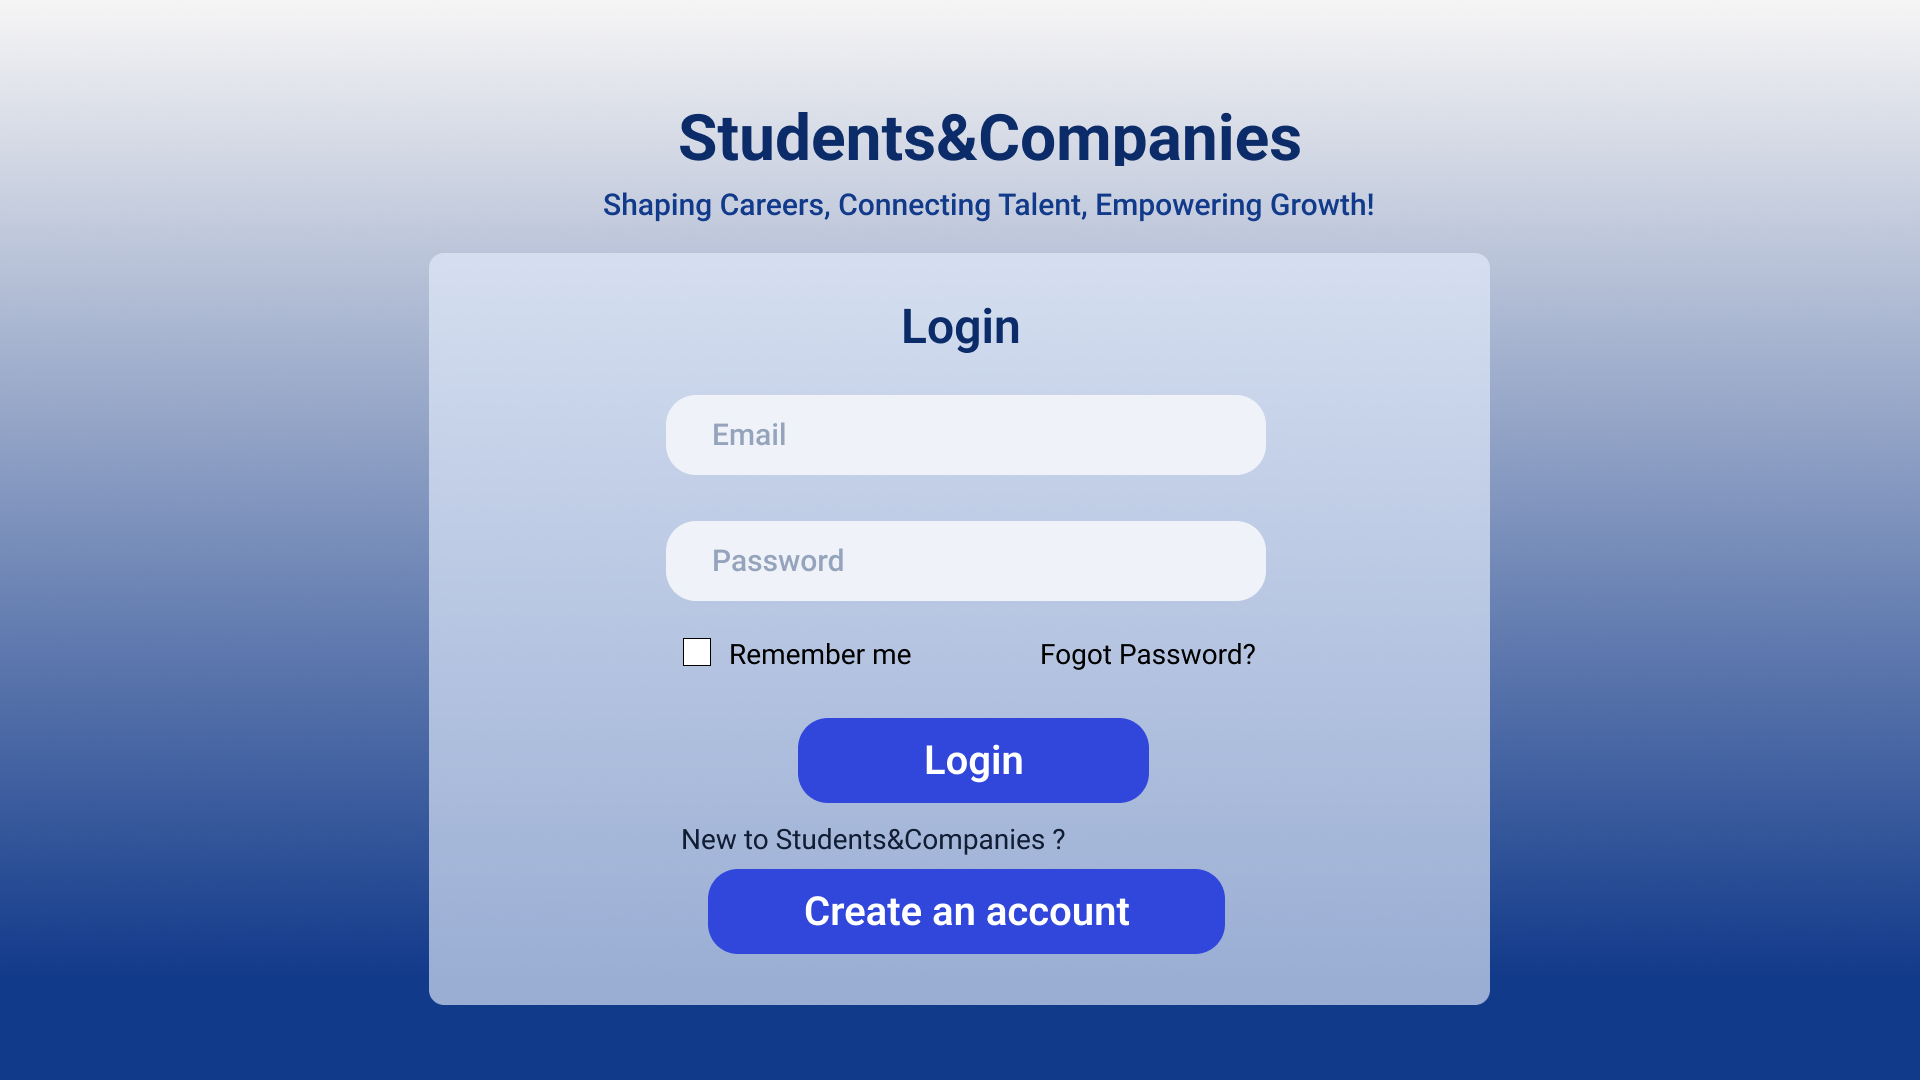
\includegraphics[width=0.8\textwidth]{Images/UI/Welcome Page.png}
    \caption{Welcome Page}\label{fig:Welcome_page}
\end{figure}

\subsection{Register Page}
If the User is not registered and wants to create an account, they will be asked to choose the type of account they want to create. 
Clicking on the type listed will redirect to the corresponding Register Page where the user can fill in the required information.
\begin{figure}[H]
    \centering
    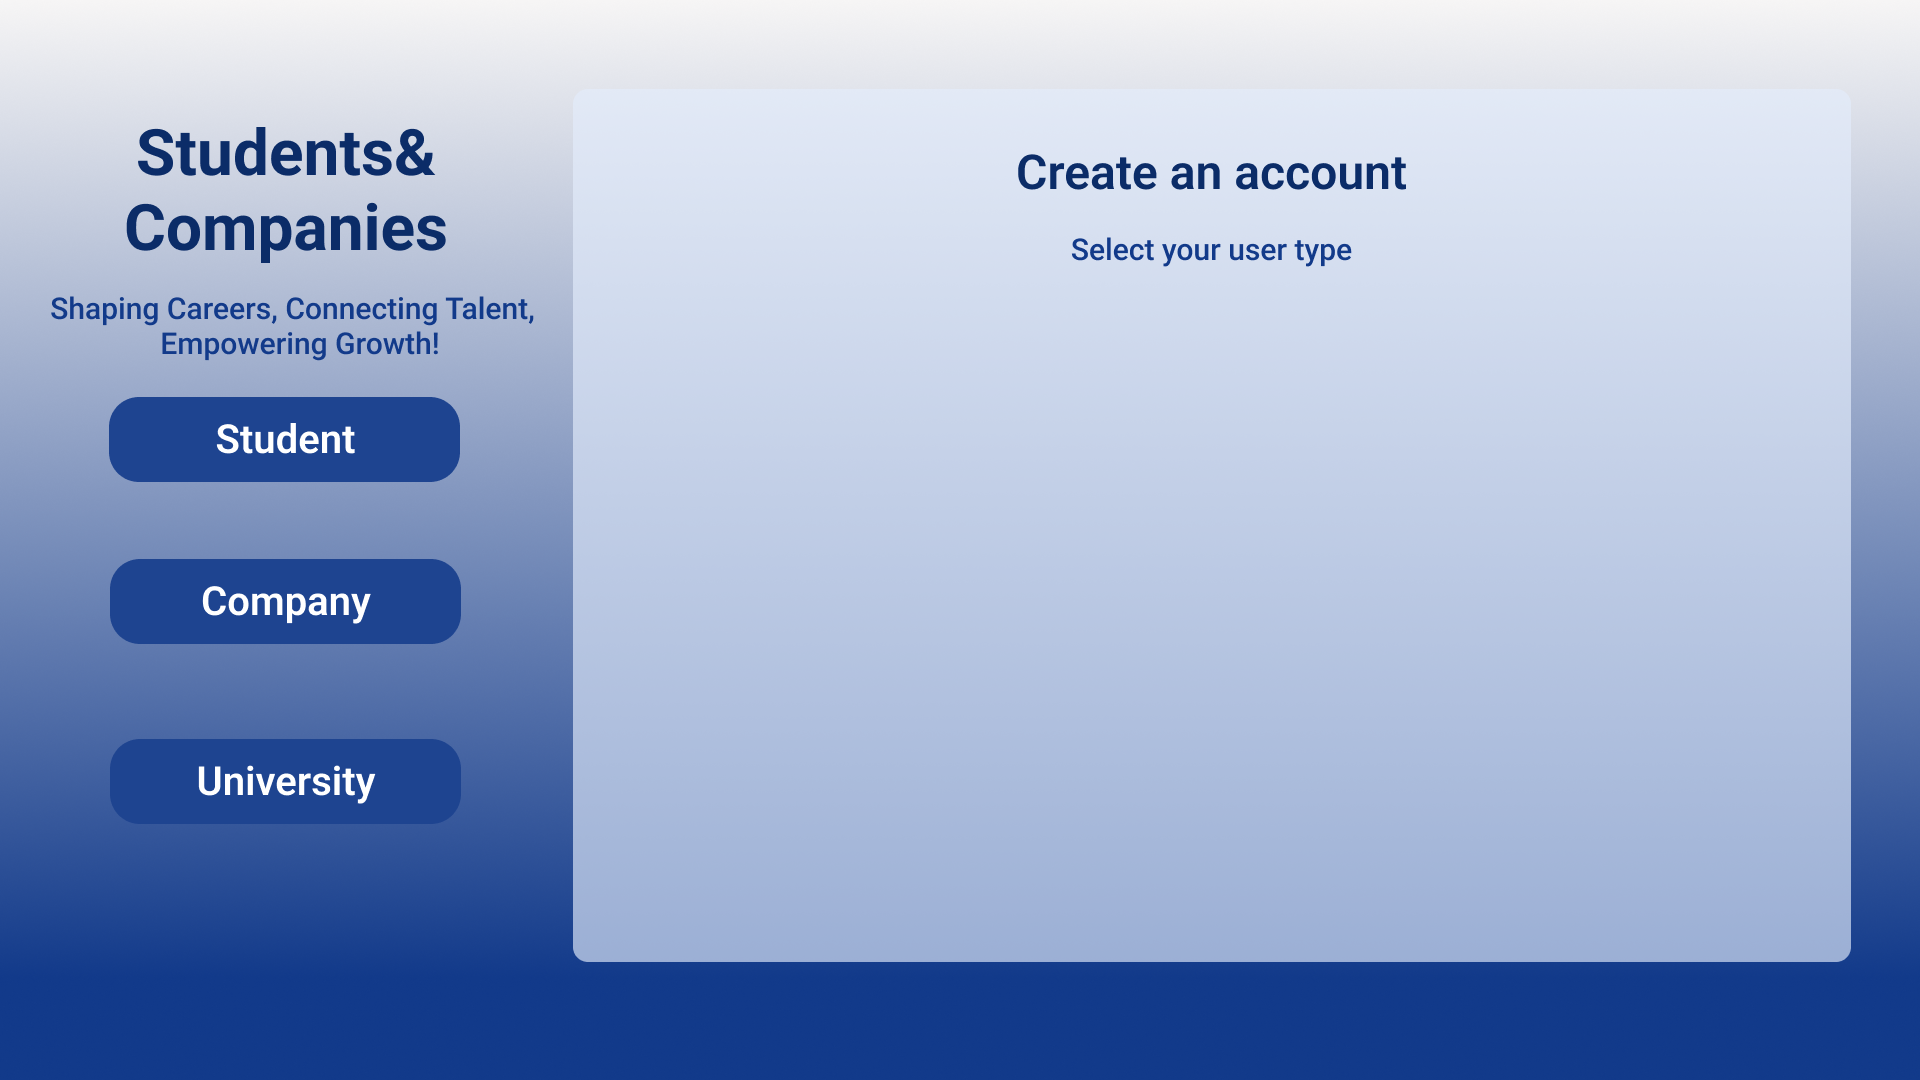
\includegraphics[width=0.8\textwidth]{Images/UI/Create account.png}
    \caption{Register Page}\label{fig:Creat_account}
\end{figure}

\begin{figure}[H]
    \centering
    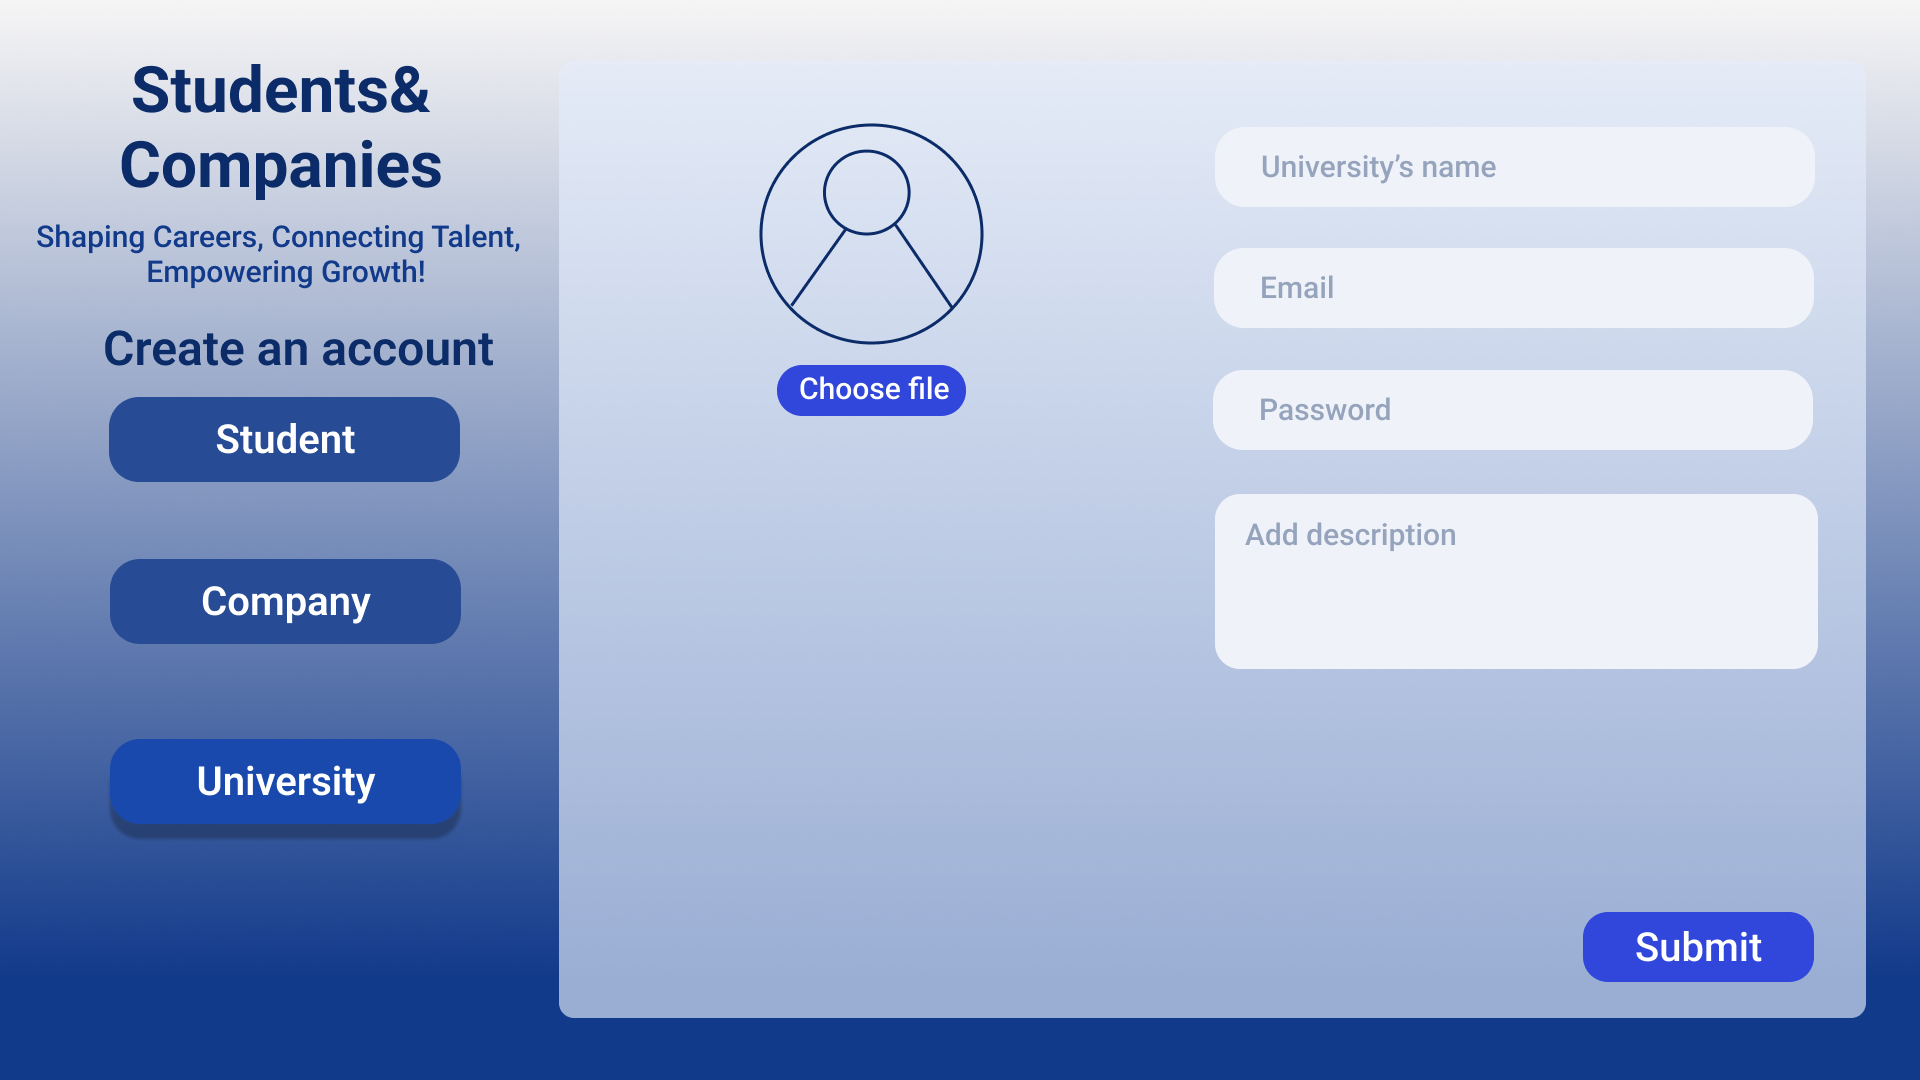
\includegraphics[width=0.8\textwidth]{Images/UI/Create account University.png}
    \caption{University create account}\label{fig:Creat_account University}
\end{figure}

\begin{figure}[H]
    \centering
    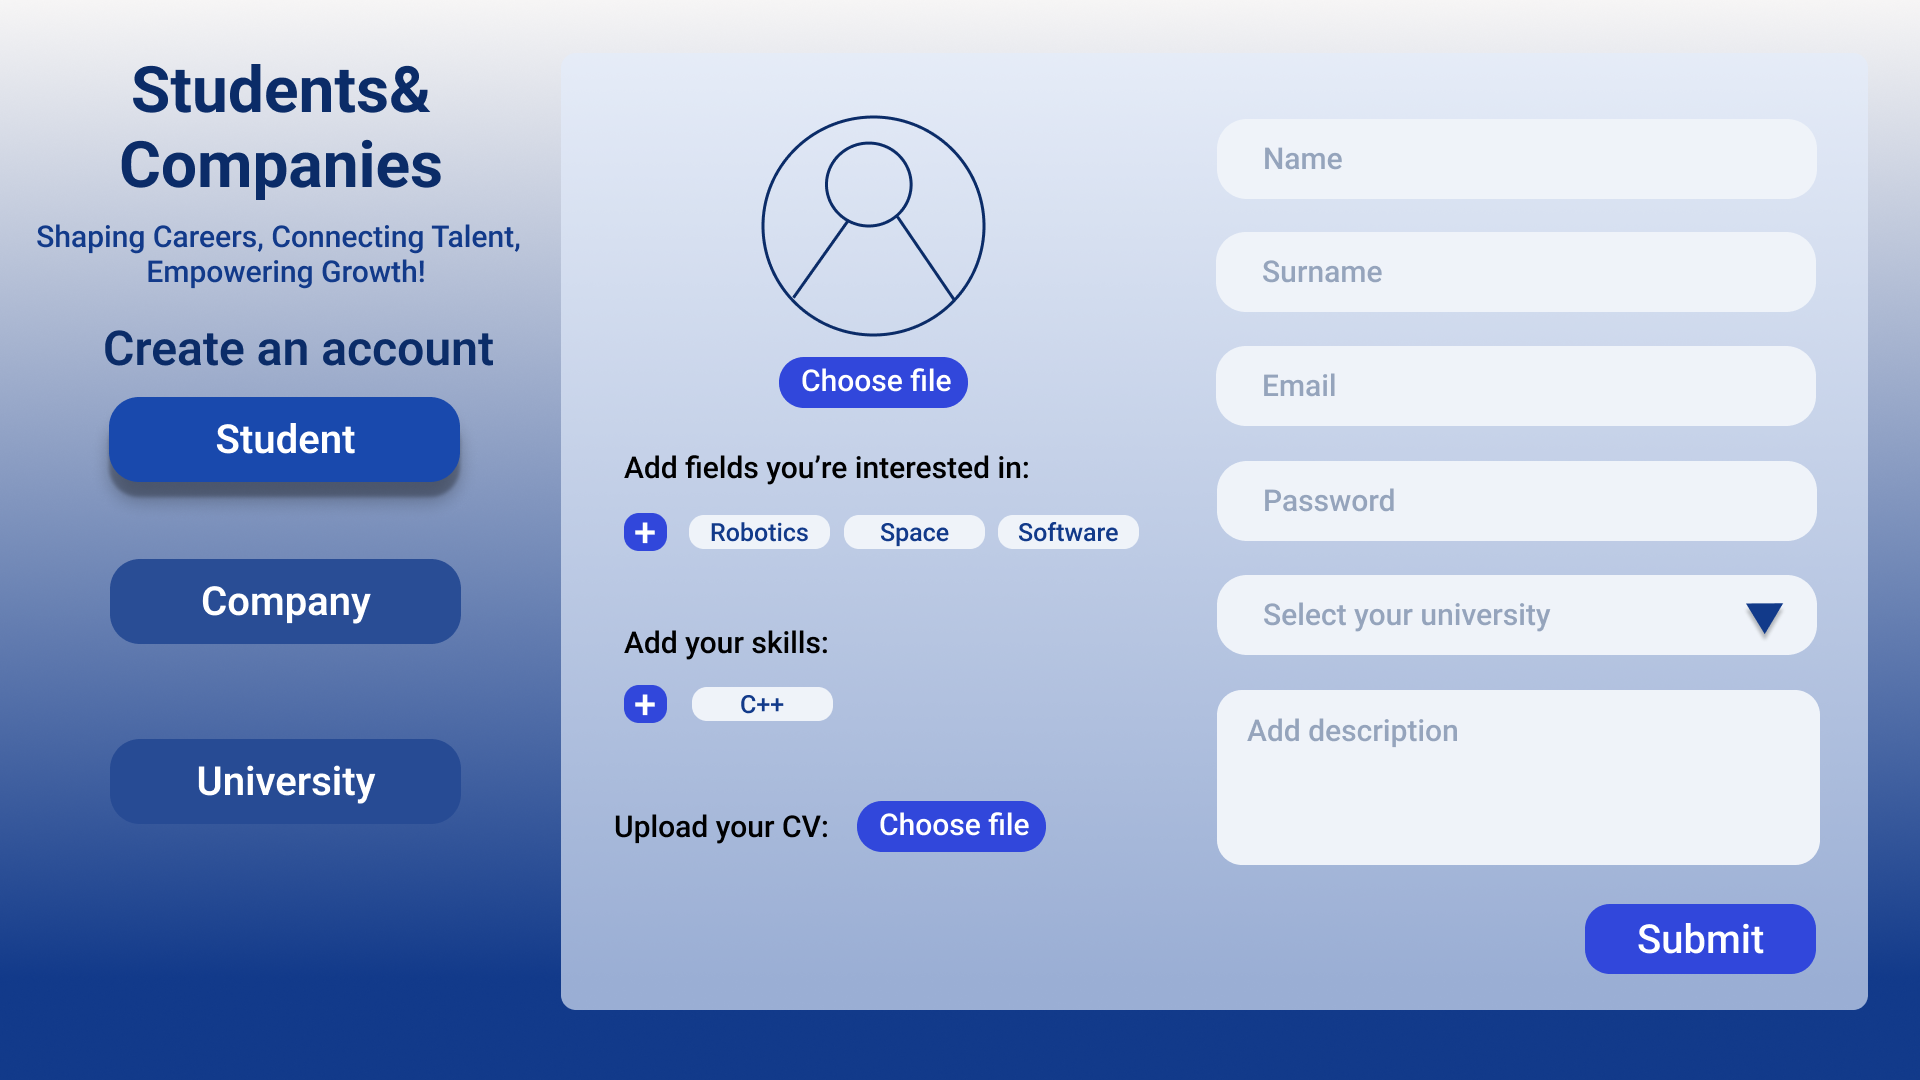
\includegraphics[width=0.8\textwidth]{Images/UI/Create account student.png}
    \caption{Student create account}\label{fig:Creat_account student}
\end{figure}

\begin{figure}[H]
    \centering
    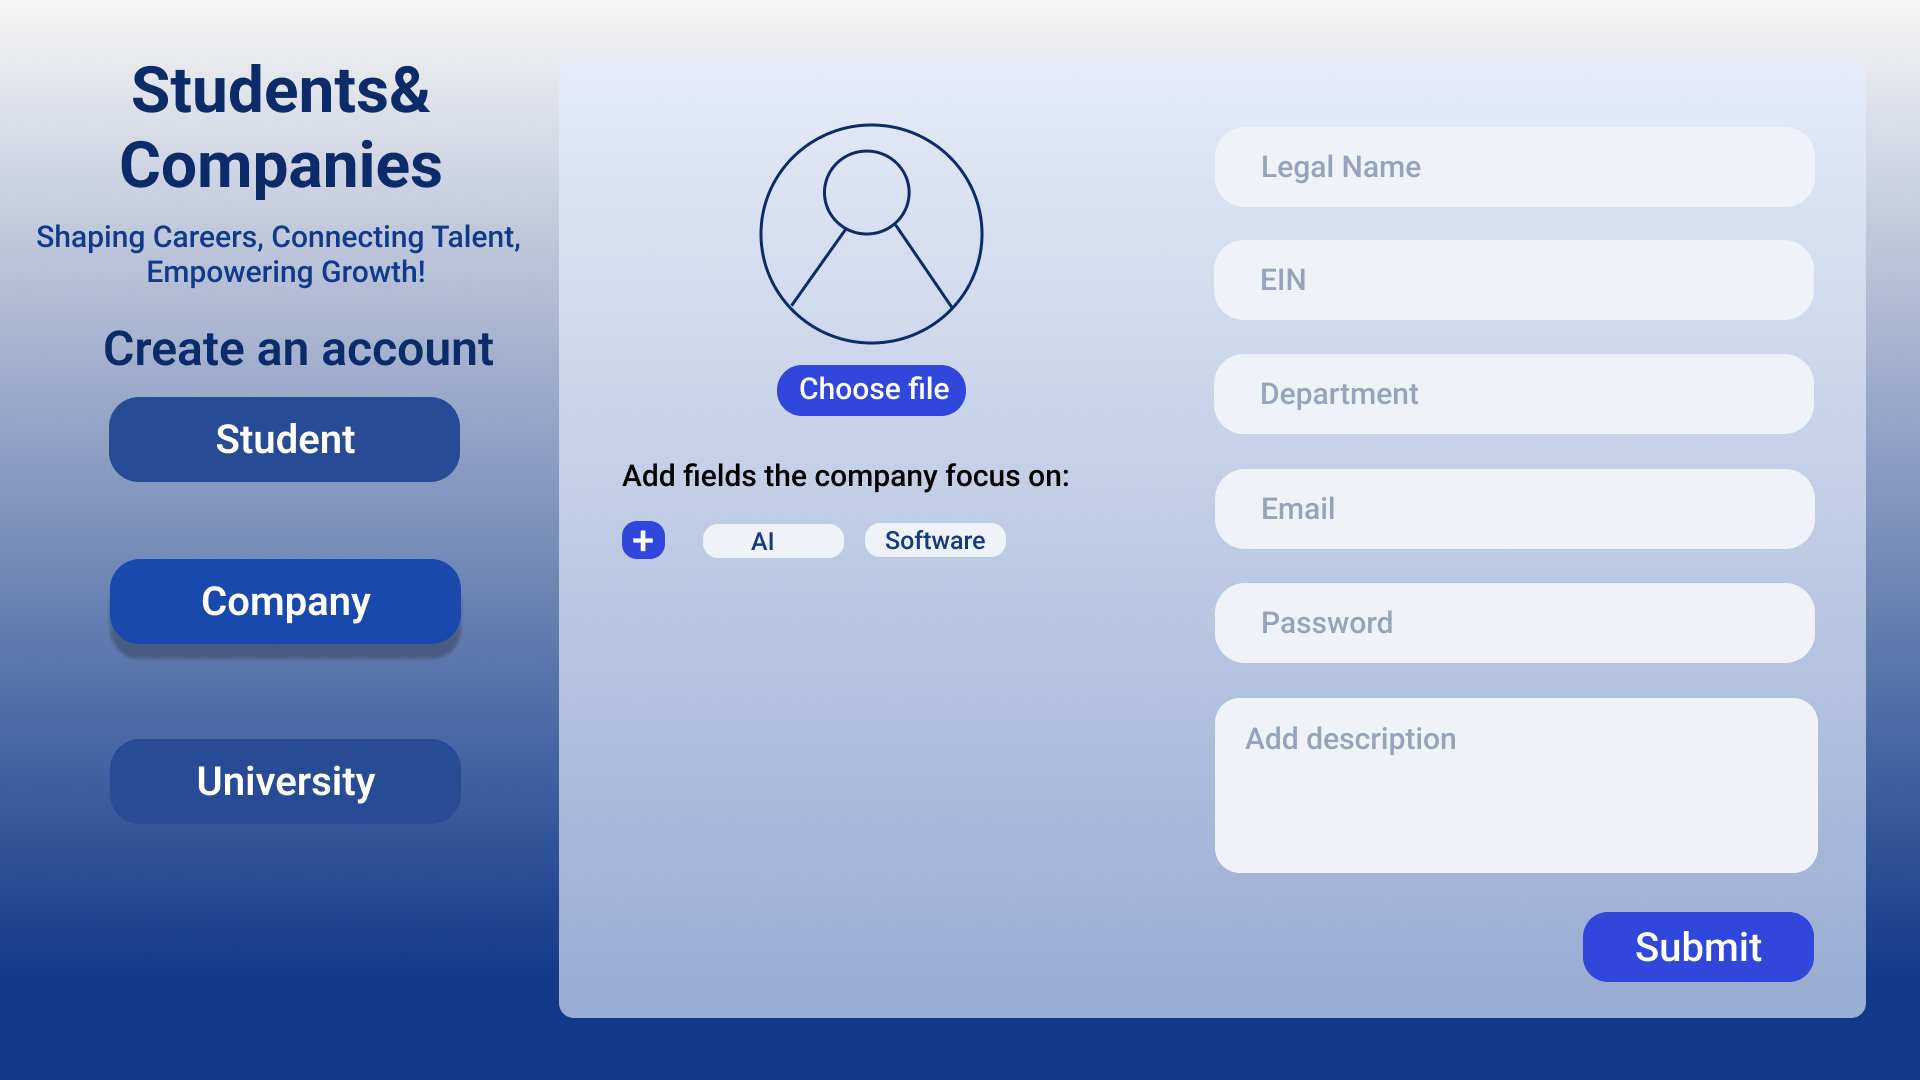
\includegraphics[width=0.8\textwidth]{Images/UI/Create account company.png}
    \caption{Company create account}\label{fig:Creat_account company}
\end{figure}
\subsection{Header bar}
The header bar is displayed on every page of the platform and contains the logo of the platform, 
the side menu button, the notification bell, and the user profile button. In particular, there 
is also the chat icon that allows the Student and Company to access available chat lists.

\subsection{Student's view}
Once access to the platform, to optimizing the user experience, the student will be able to use the side menu to navigate to the desired page:
\textit{Search, Dashboard, My applications and My internships}.
\begin{figure}[H]
    \centering
    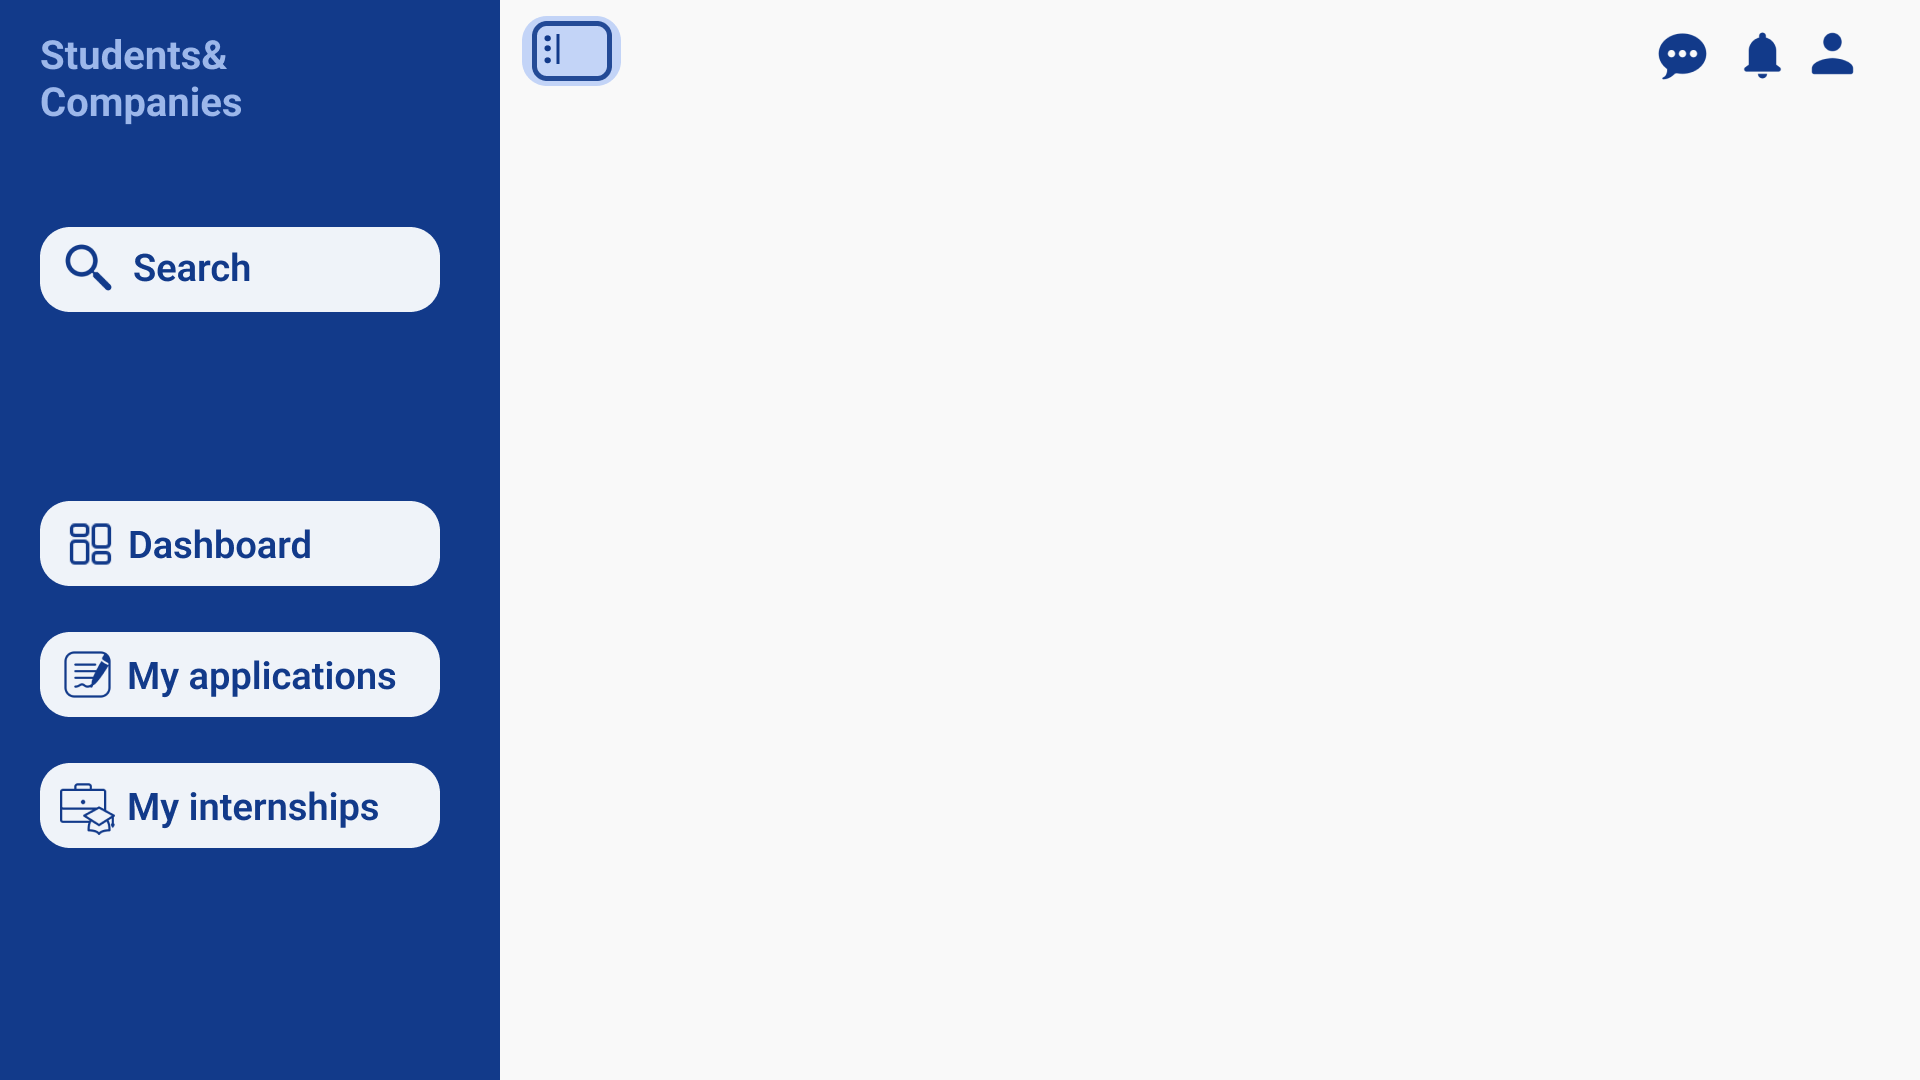
\includegraphics[width=0.8\textwidth]{Images/UI/Layout-Student.png}
    \caption{Student's Side Menu}\label{fig:Student_view}
\end{figure}
\subsubsection{Dashboard page}
By default, students are directed to the Dashboard page upon logging in.\\ 
The Dashboard provides an overview that allows students to quickly assess 
the current status of their applications and the performance of internships they are participating in or have completed.
Clicking on a specific application or internship within the overview list redirects students to a detailed page for that application or internship.\\
Next to the historical internship section, there is a window displaying the latest comments on the current internship with quick access to 
the Feedback and Complaint pages for the ongoing internship, click on \textit{Open}.\\
Additionally, students can use the search bar to find internships or user profiles by entering relevant keywords. Below the search bar, there is a
 \textit{Suggested Job Searches} section, where students can click on a keyword to quickly search for internships that match their interests.
Below this section, a list of recommended internship announcements tailored to the student is displayed. Each announcement includes a brief description, 
and students can take one of three actions:
\begin{itemize}
    \item[-] Click the \textit{Apply Now} button to apply for the internship.
    \item[-] Click the block to view more details about the internship announcement.
    \item[-] Click the \textit{X} to remove the internship announcement from the display.
\end{itemize}
\begin{figure}[H]
    \centering
    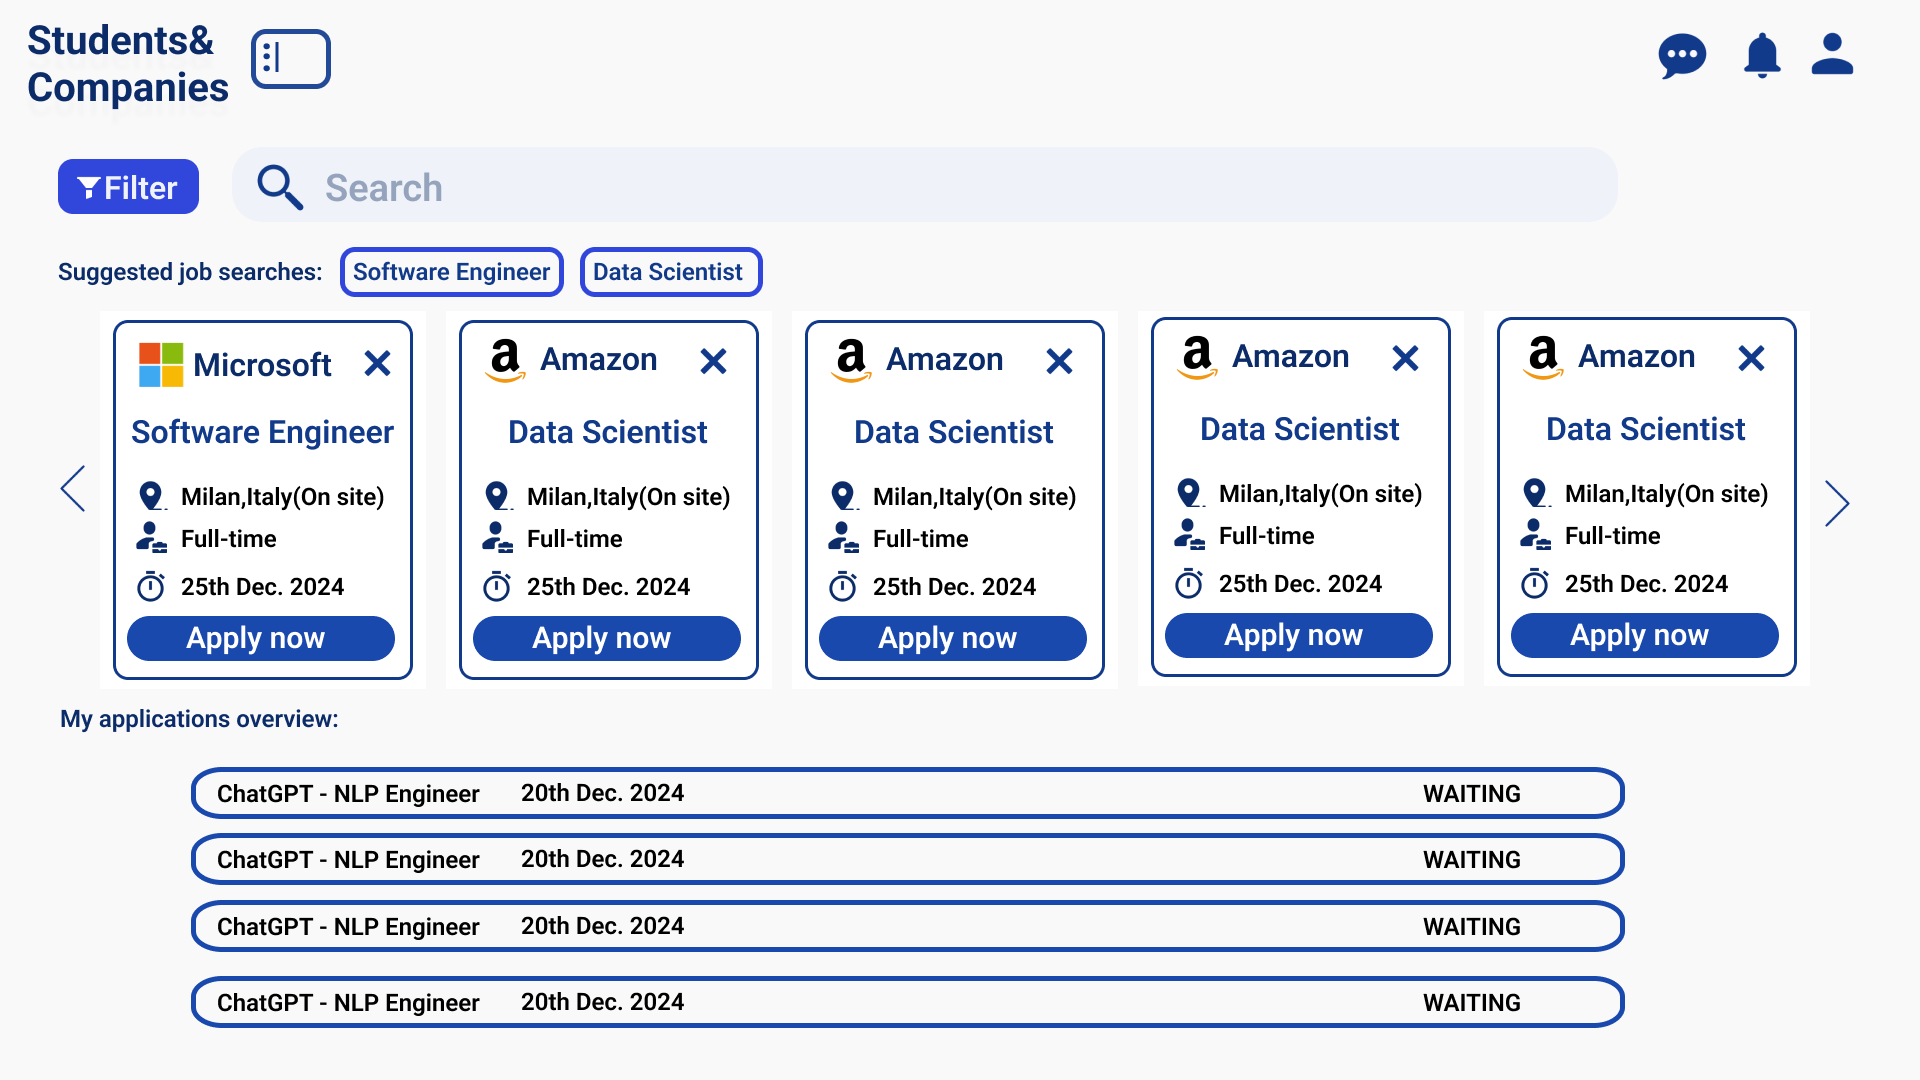
\includegraphics[width=0.8\textwidth]{Images/UI/Dashboard 1-student.png}
    \caption{Student's Dashboard 1}\label{fig:DashboardStudent1}
\end{figure}

\begin{figure}[H]
    \centering
    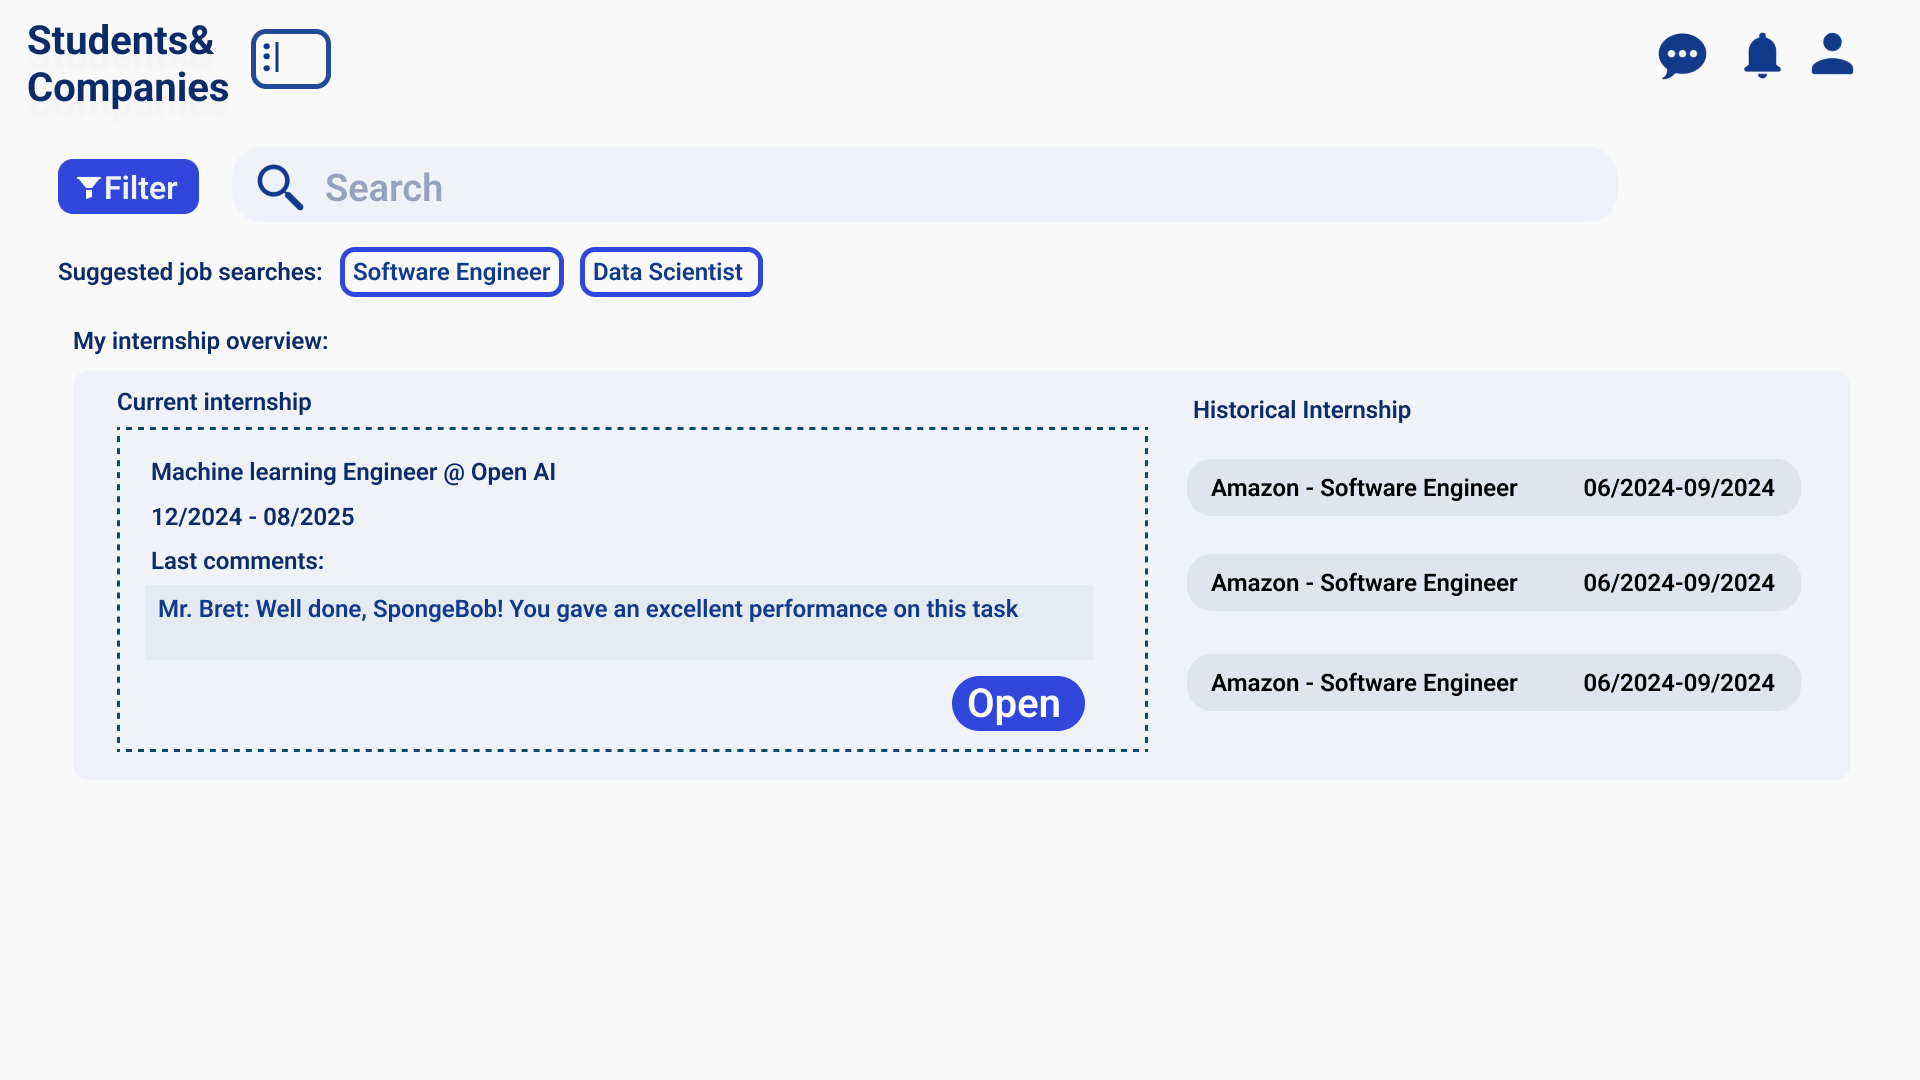
\includegraphics[width=0.8\textwidth]{Images/UI/Dashboard 2-student.png}
    \caption{Student's Dashboard 2}\label{fig:Dashboard Student 2}
\end{figure}
\subsubsection{My application page}
Here in figure\ref{fig:My application}, the student can view the status of their applications and take action based on the status of the application:
\begin{itemize}
    \item[-] Click on the \textit{View details} button to view the page with details of the internship announcement, figure\ref{fig:Internship announcement details}.
    \item[-] Click on the \textit{Invited to interview} button to view the details of the interview and questionnaire requested by the company to fill in, figure\ref{fig:Interview details 1}.
    \item[-] Click on the \textit{Accept or Reject Offer} button to view the details offer letter and to take the decision to accept or reject the offer, figure\ref{fig:Accept or Reject Offer}.
\end{itemize}
\begin{figure}[H]
    \centering
    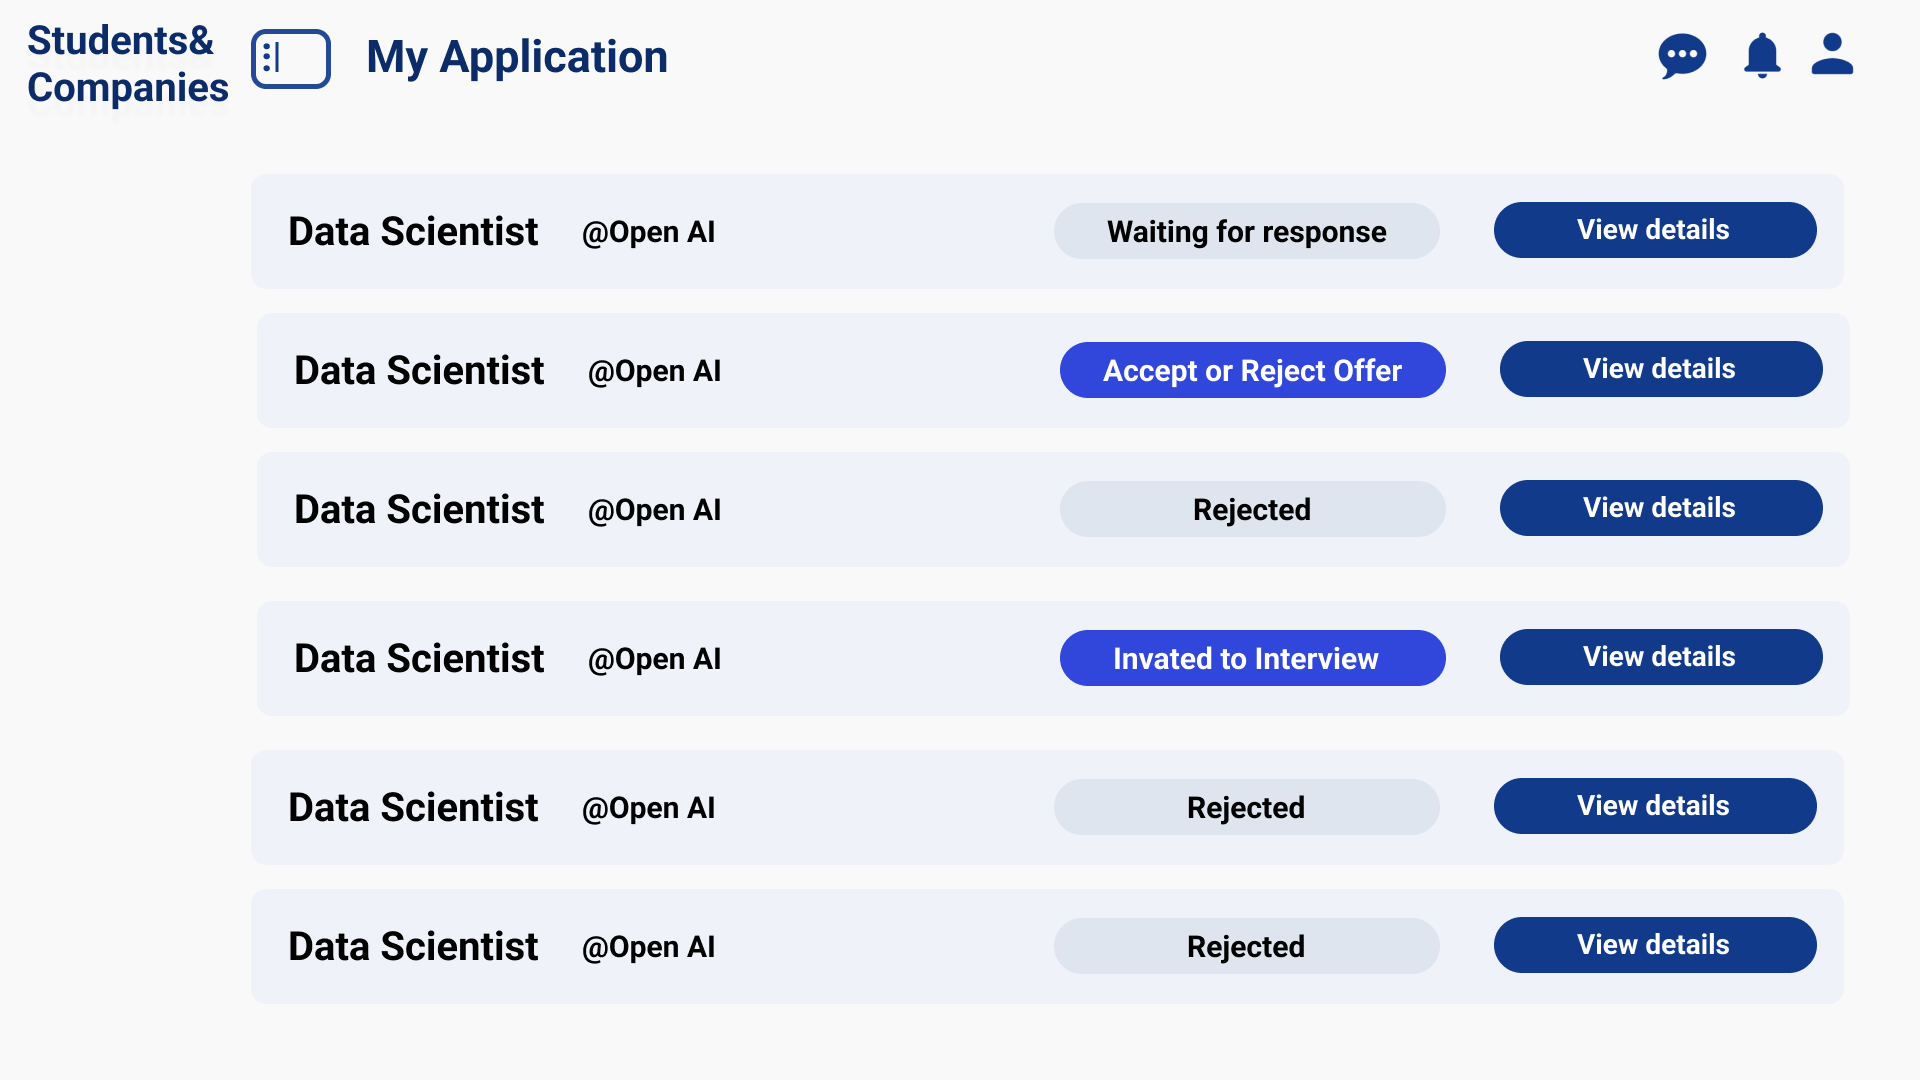
\includegraphics[width=0.8\textwidth]{Images/UI/My Application-student.png}
    \caption{My application}\label{fig:My application}
\end{figure}
\subsubsection{Interview details page}
Show the detail information related to the interview and the pre-interview questionnaire asked by the company to candidate to fill in.\\
Once completed all questions with the provided answers, the student can click on the \textit{Submit} button to send the answers to the company and save the answers in the platform for future reference.
\begin{figure}[H]
    \centering
    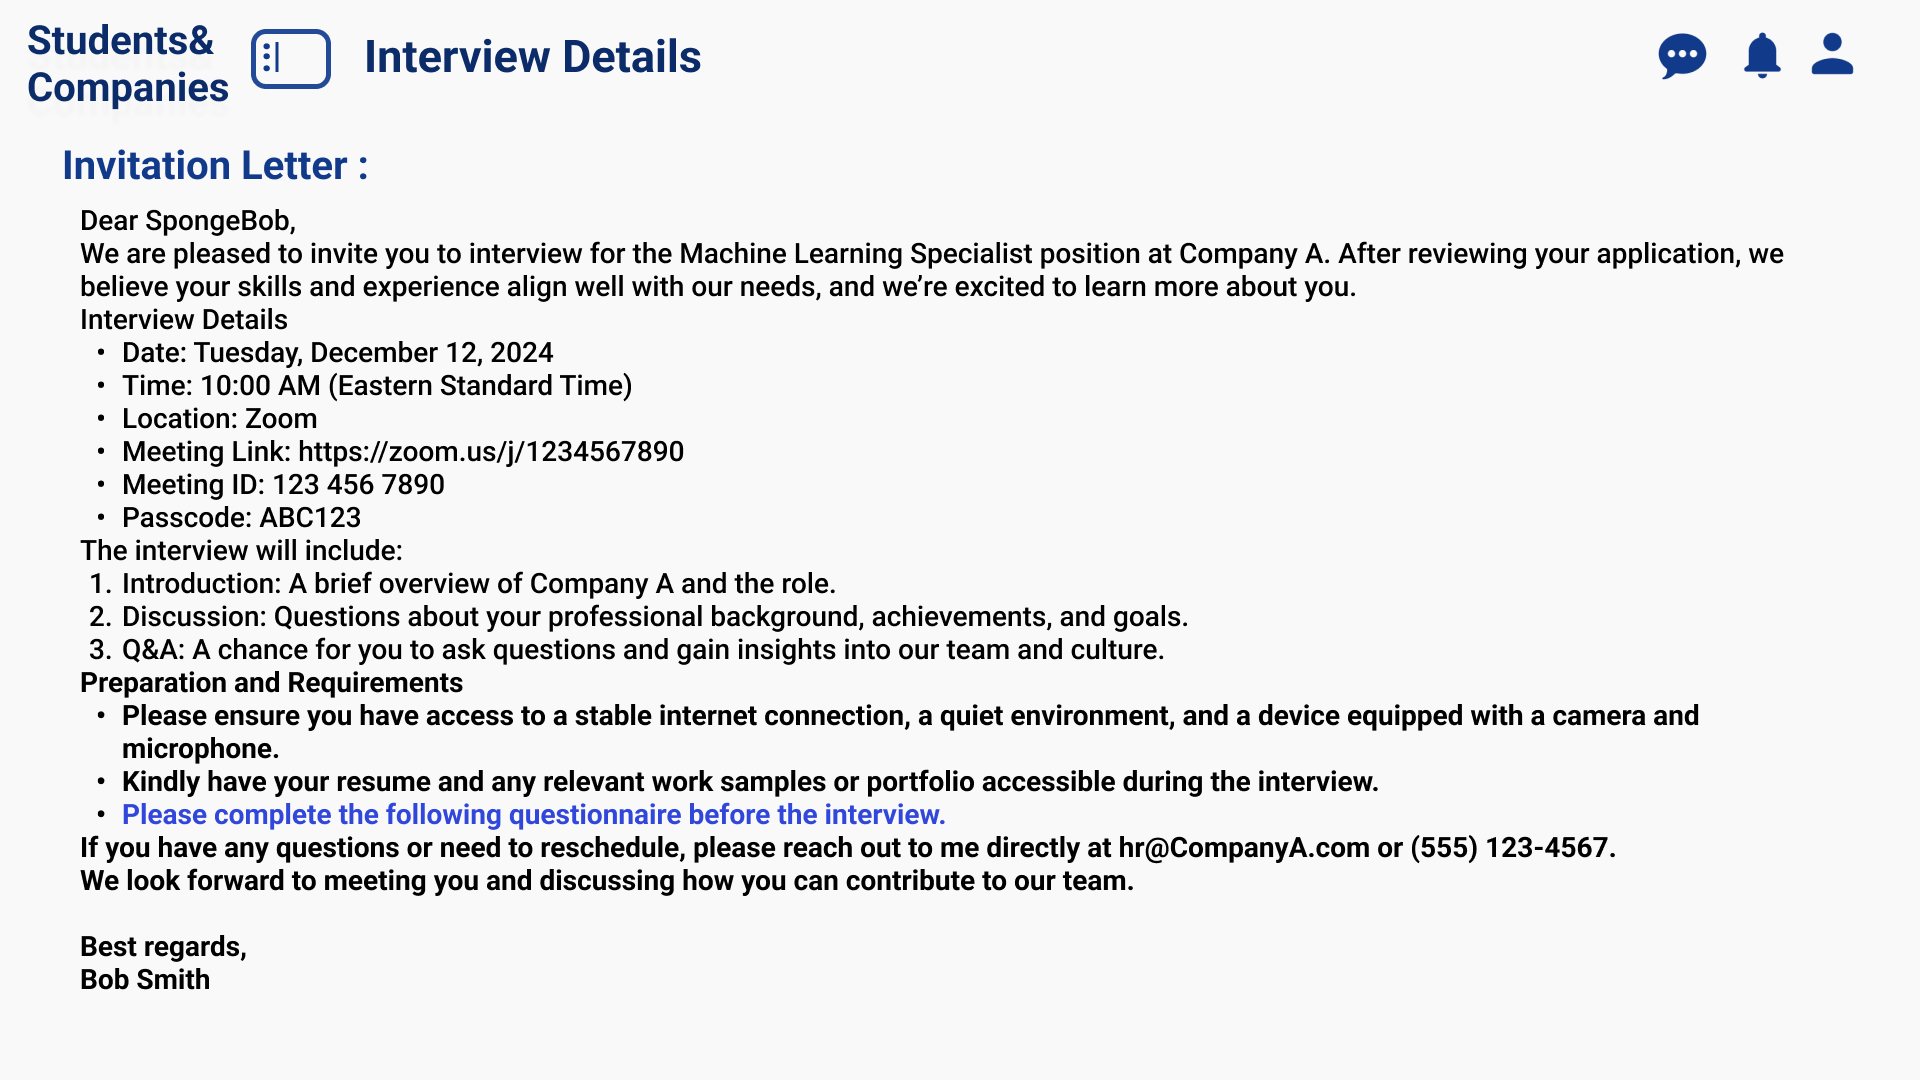
\includegraphics[width=0.8\textwidth]{Images/UI/Interview Details-student.png}
    \caption{Interview details 1}\label{fig:Interview details 1}
\end{figure}

\begin{figure}[H]
    \centering
    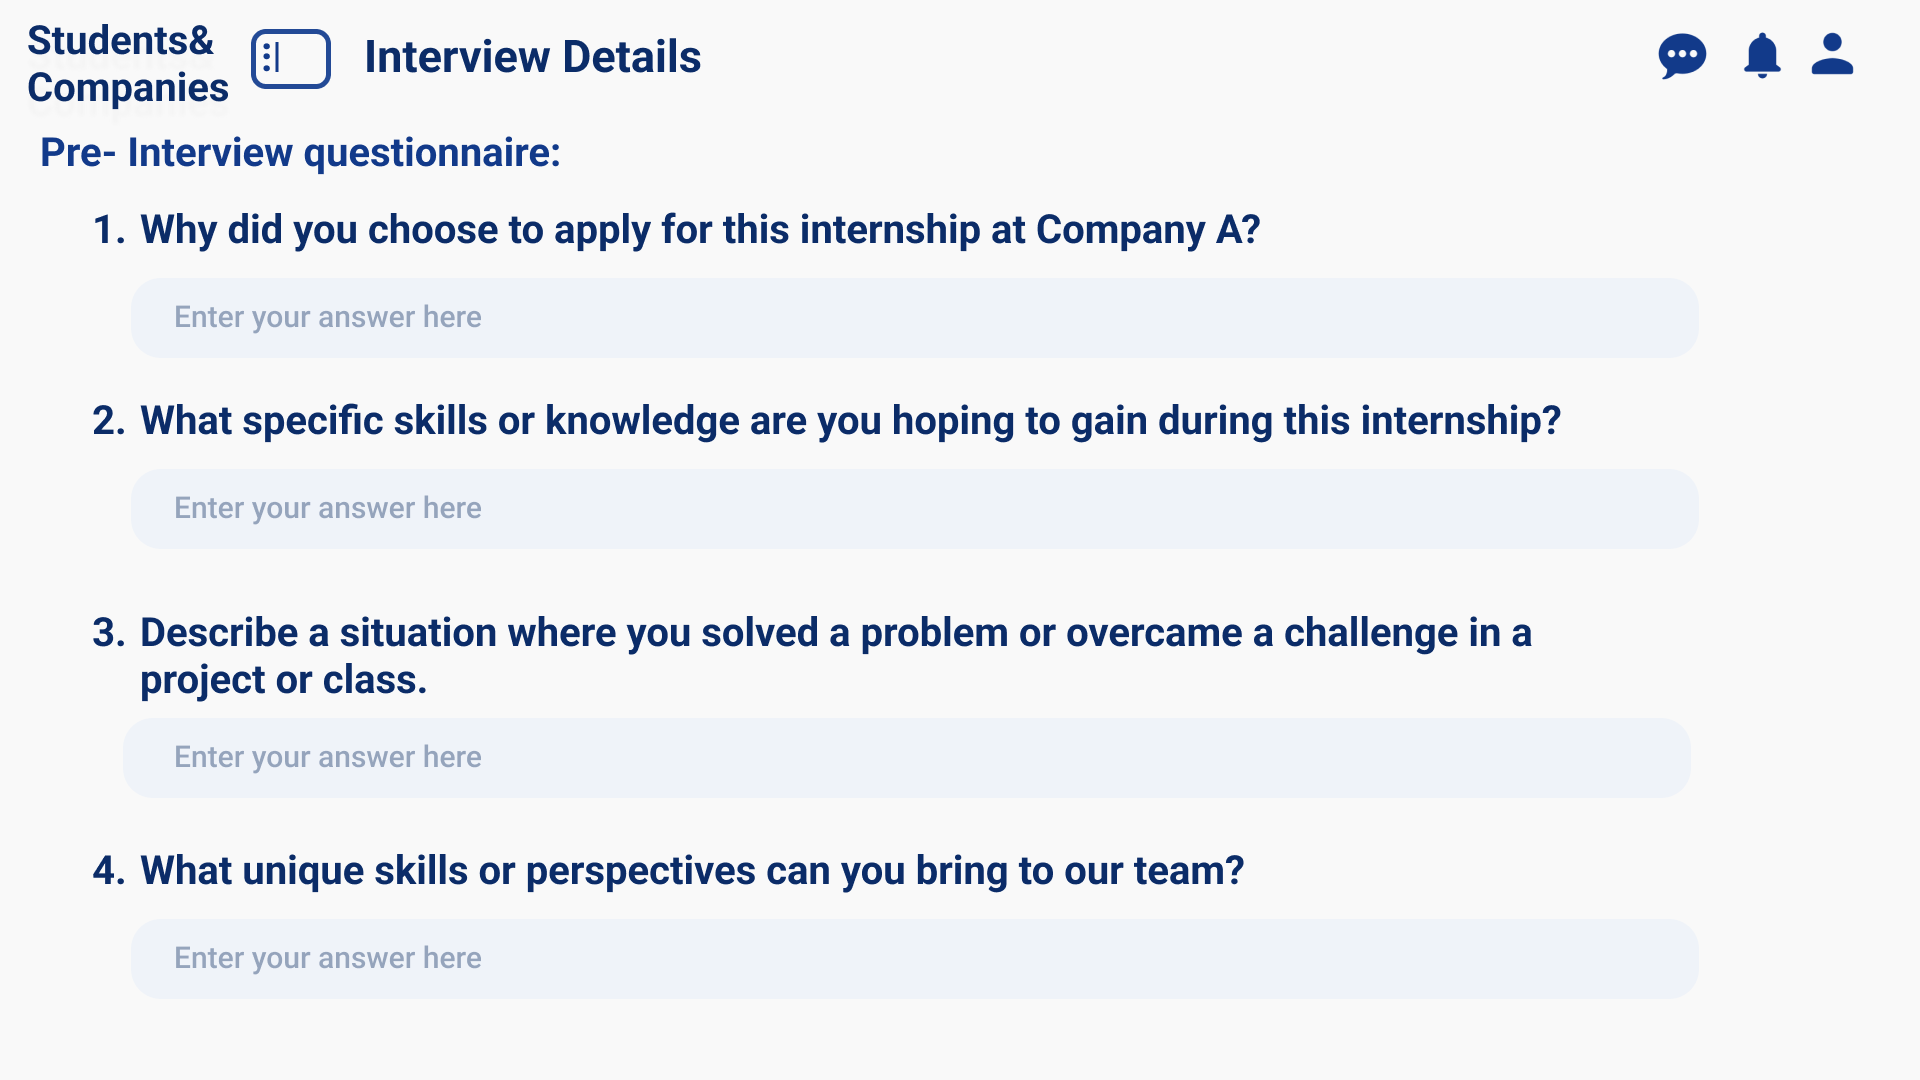
\includegraphics[width=0.8\textwidth]{Images/UI/Interview Details2-student.png}
    \caption{Interview details 2}\label{fig:Interview details 2}
\end{figure}

\begin{figure}[H]
    \centering
    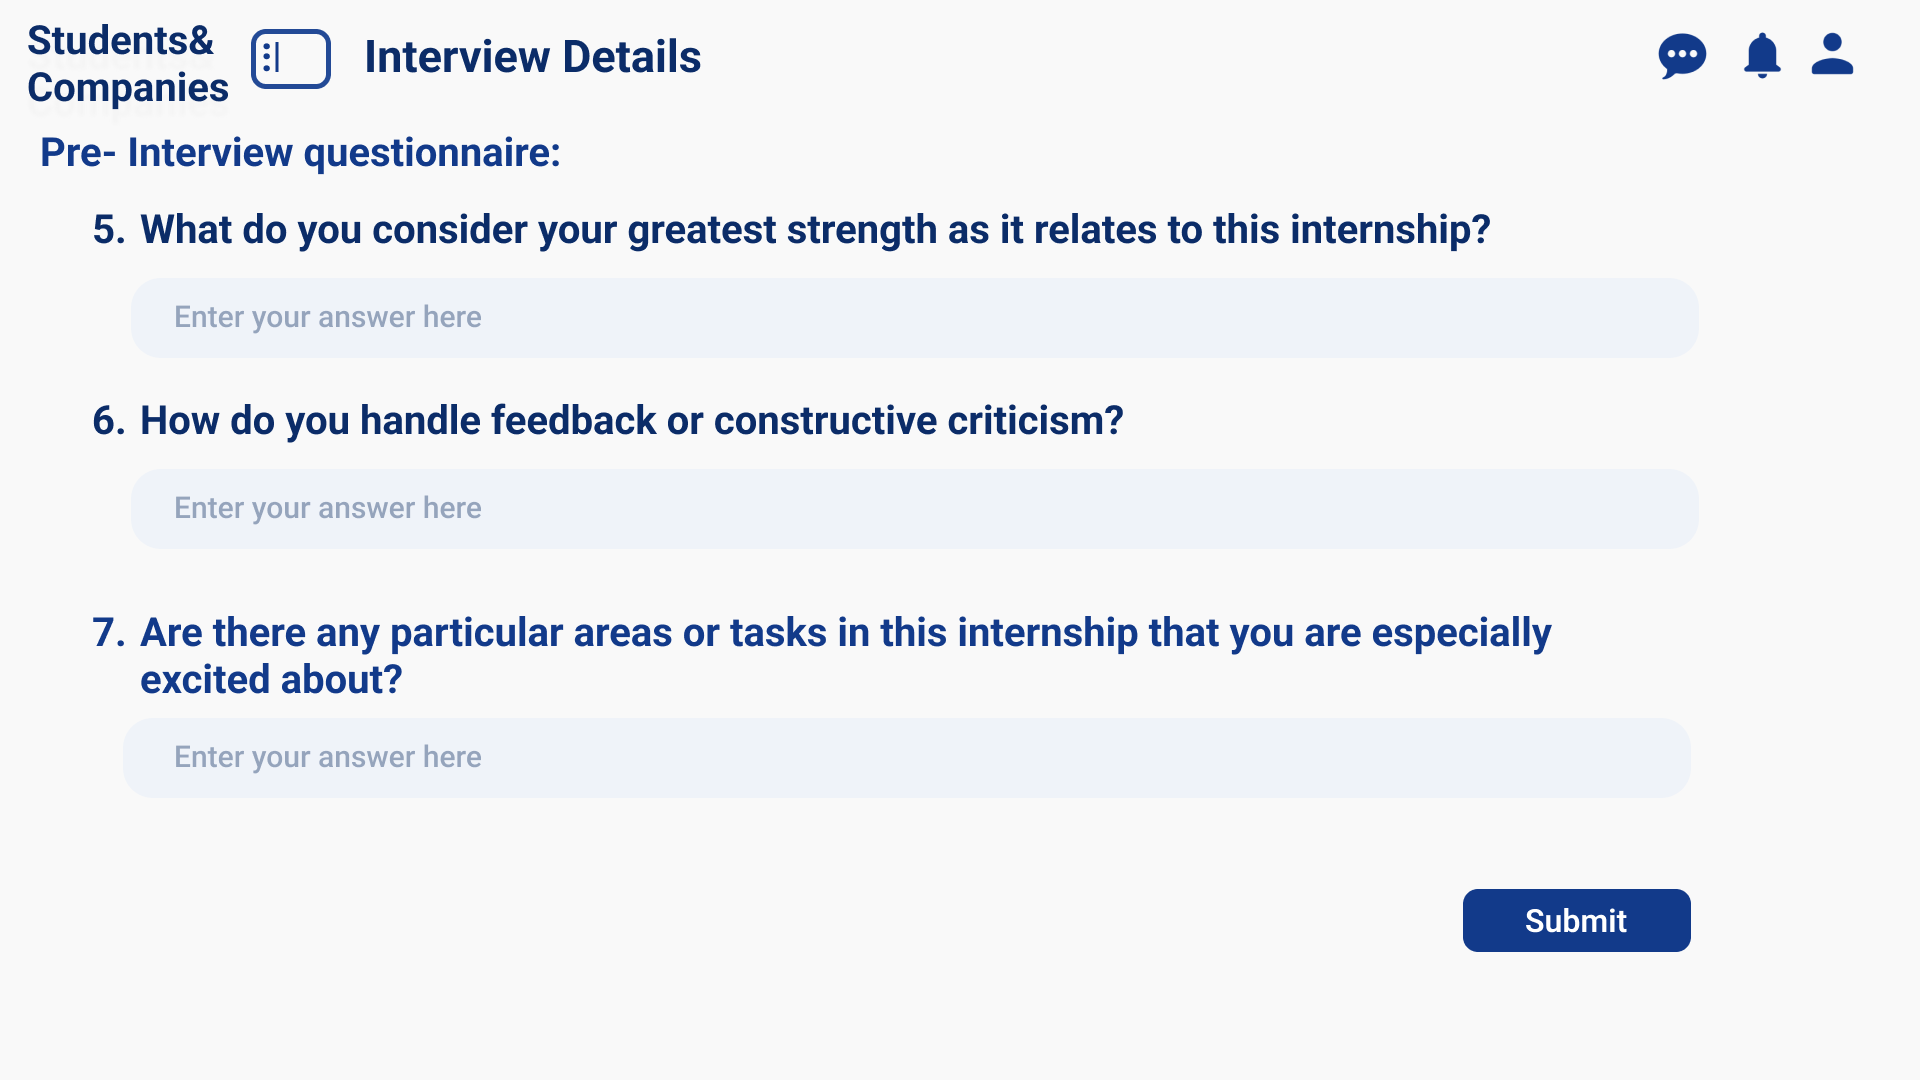
\includegraphics[width=0.8\textwidth]{Images/UI/Interview Details3-student.png}
    \caption{Interview details 3}\label{fig:Interview details 3}
\end{figure}
\subsubsection{Offer page}
Provide the offer letter sent by the company to the student. The student can take the decision to accept or reject the offer by clicking on the corresponding button.
Then the student decision will be sent to the company and recorded in the database, the application status will be updated accordingly.
\begin{figure}[H]
    \centering
    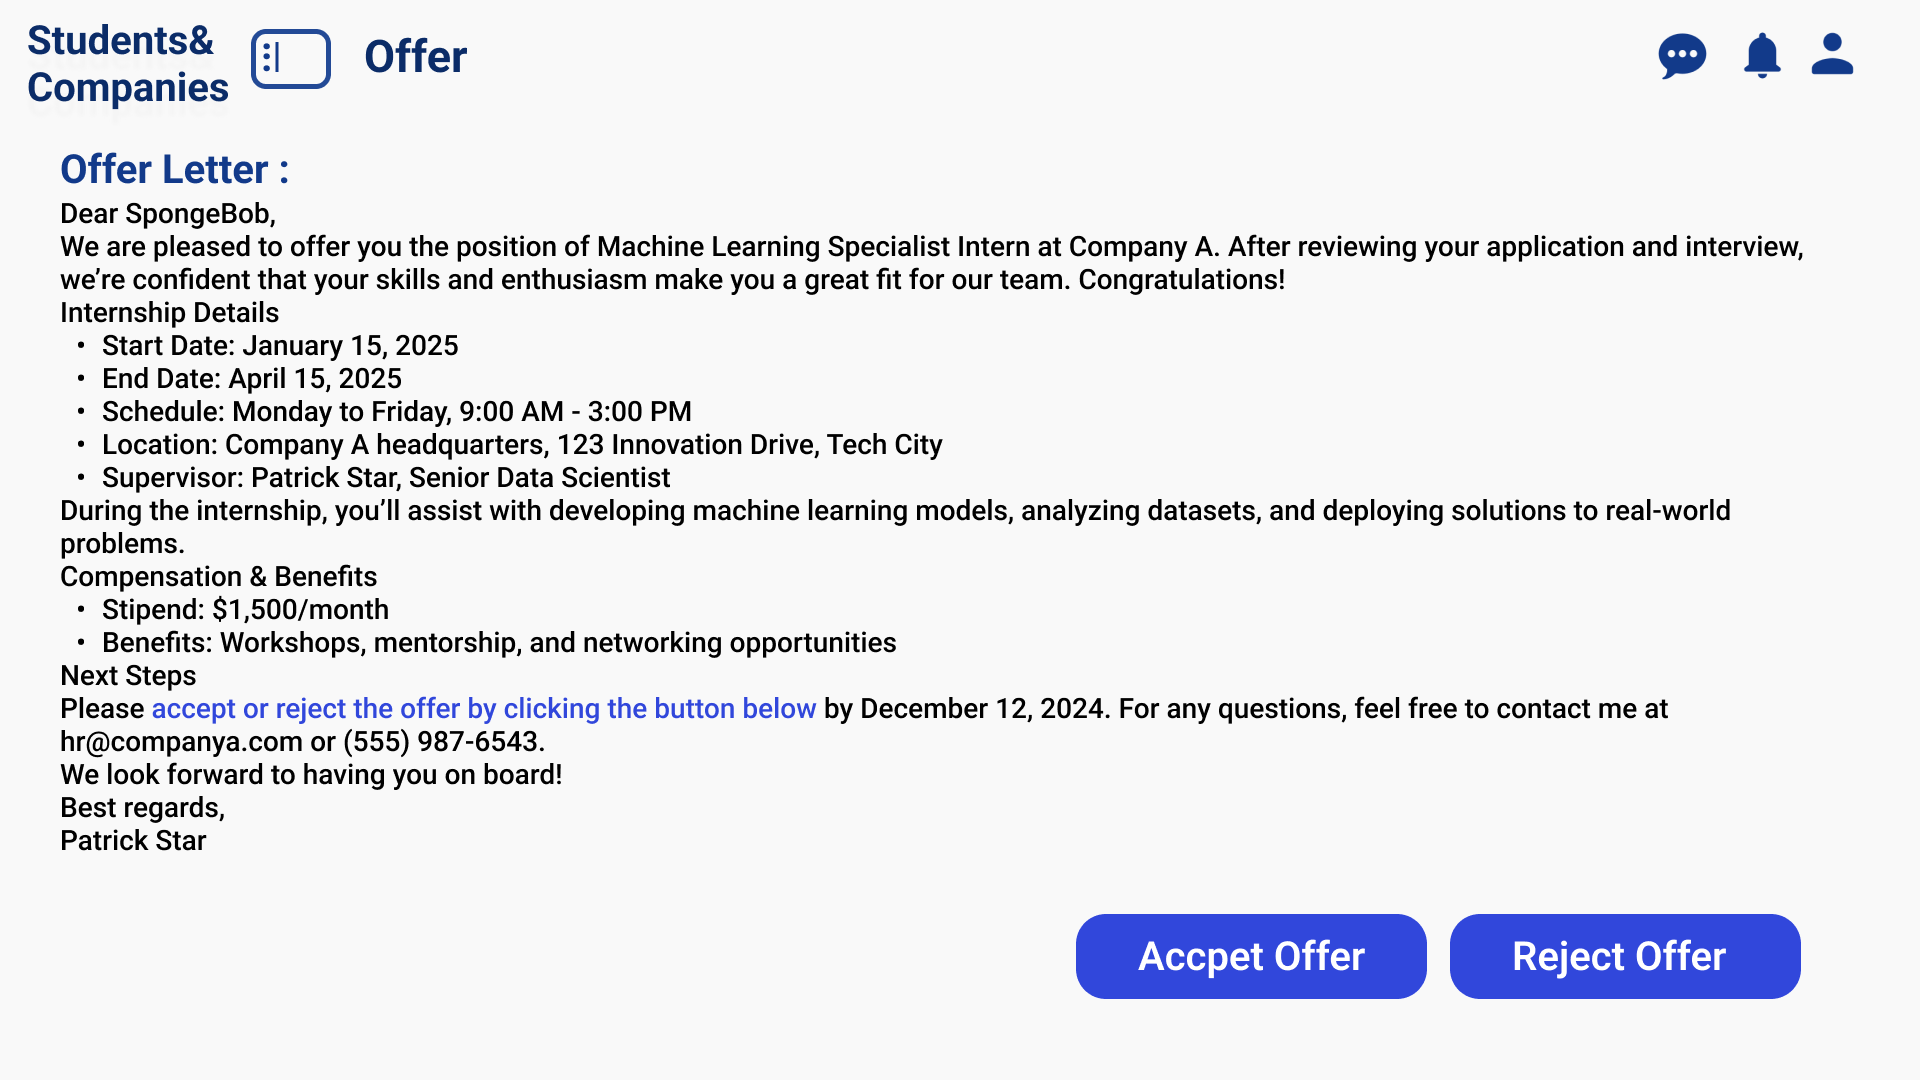
\includegraphics[width=0.8\textwidth]{Images/UI/Reject-student.png}
    \caption{Accept or Reject Offer }\label{fig:Accept or Reject Offer}
\end{figure}
\subsubsection{My internship page}
Here in figure\ref{fig:My internship}, the student can view the list of internships they are participating in or have completed.\\
For the current internship, the student can access the feedback and complaint page by clicking on the \textit{Add comments} button. \\
For the historical internship, the student can view the feedback and complaints recorded by the company and the student during the internship clicking
on the \textit{View details} button.
\begin{figure}[H]
    \centering
    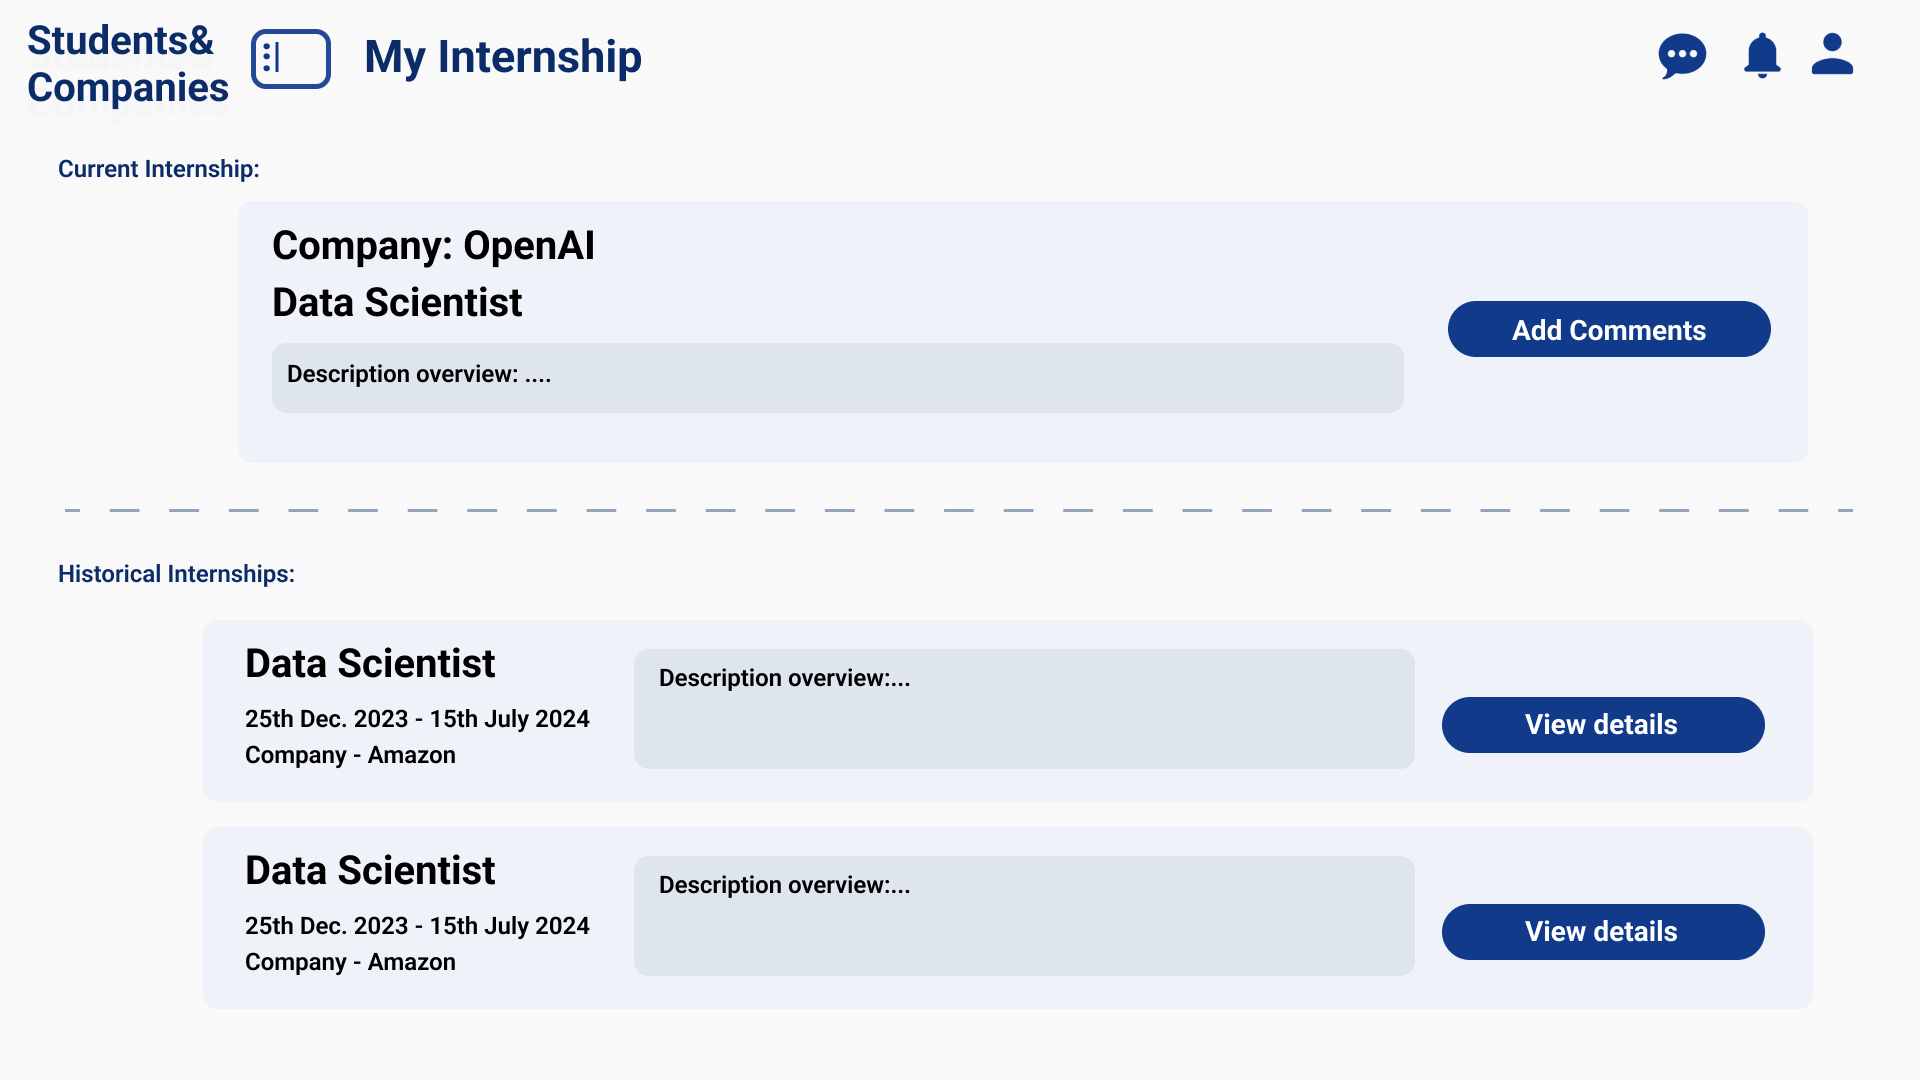
\includegraphics[width=0.8\textwidth]{Images/UI/My Internship-student.png}
    \caption{My internship }\label{fig:My internship}
\end{figure}
\subsubsection{Internship announcement page}
Represents the internship announcement details by the student's view side.
\begin{figure}[H]
    \centering
    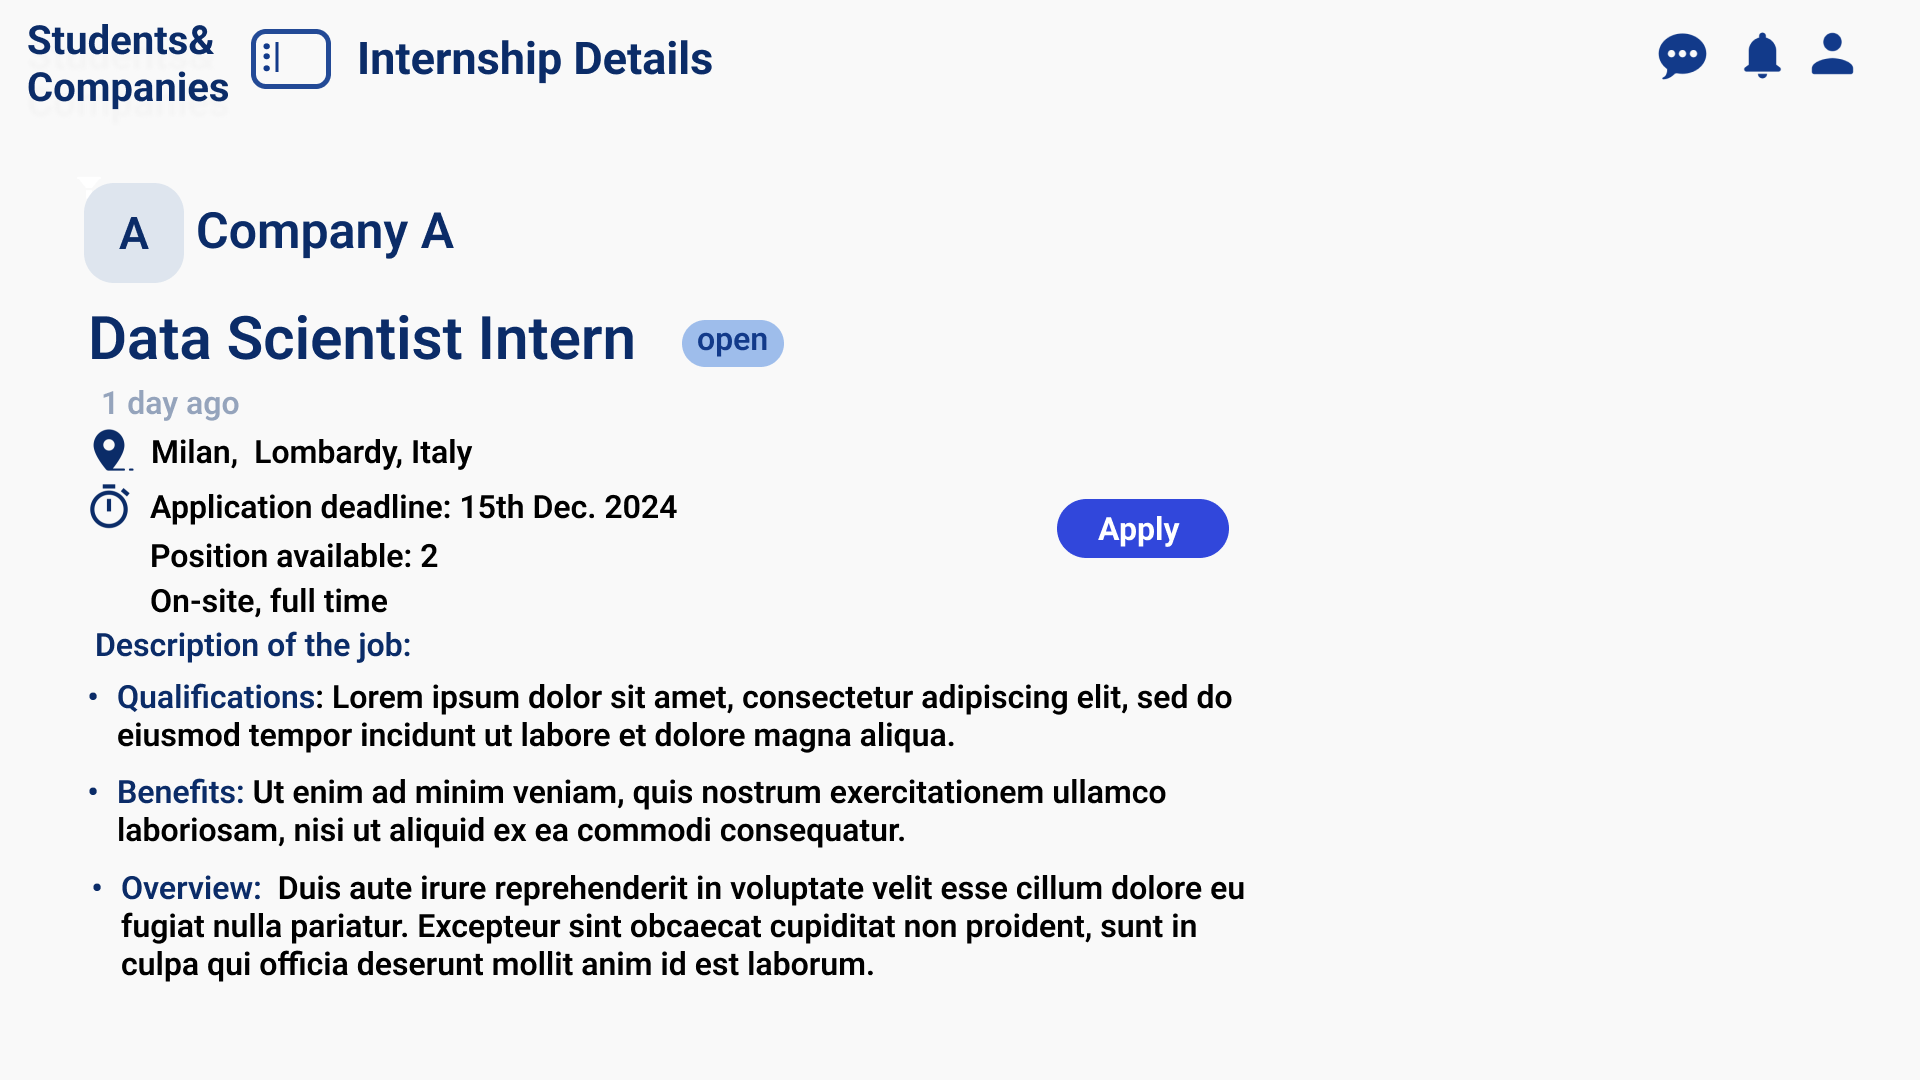
\includegraphics[width=0.8\textwidth]{Images/UI/Internship details-student view.png}
    \caption{Internship announcement details }\label{fig:Internship announcement details}
\end{figure}
\subsubsection{Student profile page}
It shows a student's profile from the prospective of other's user once looking for his/her profile.
The personal information such as profile photo, name, email and major are displayed in this page as 
well as the list of internships the student has participated. 
\begin{figure}[H]
    \centering
    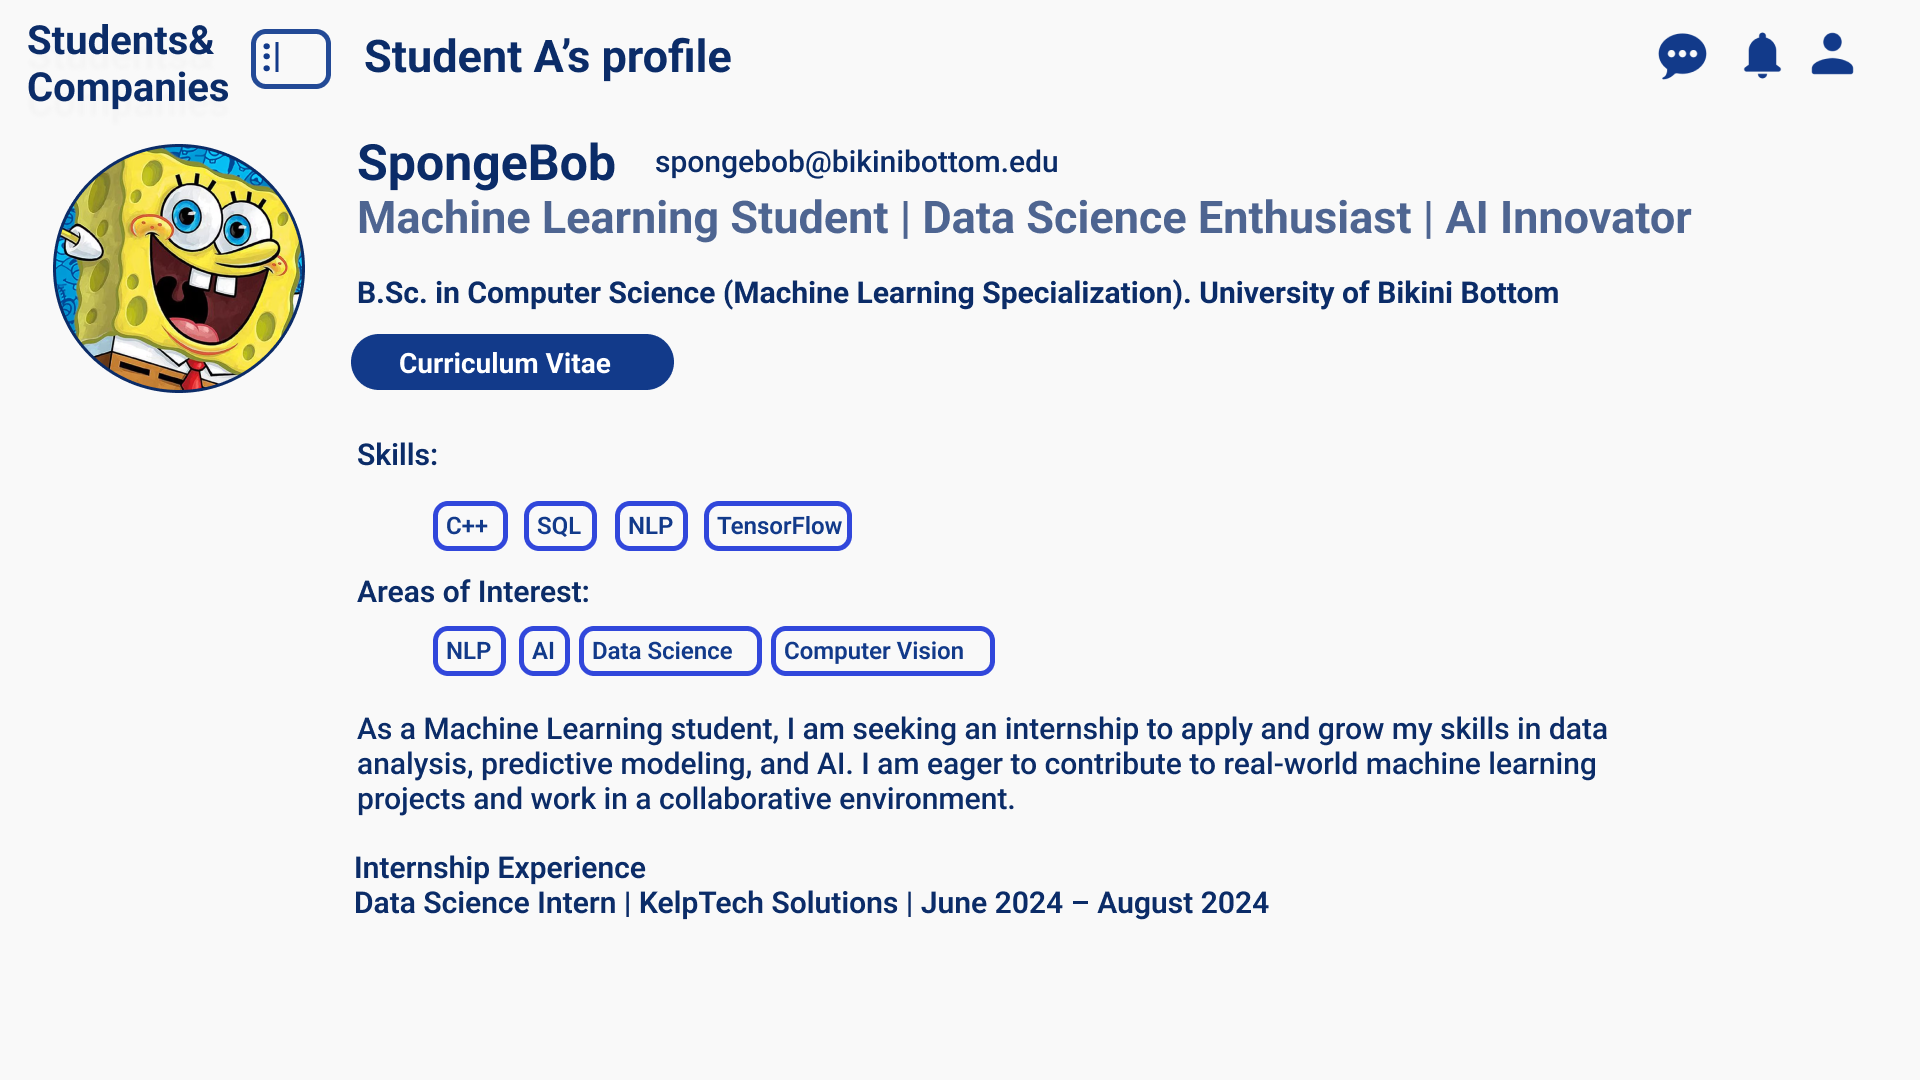
\includegraphics[width=0.8\textwidth]{Images/UI/Student profile.png}
    \caption{Student's profile from other's view}\label{fig:Student's profile from other's view}
\end{figure}

\newpage
\subsection{Company's view}
As the student, the company can use the side menu to navigate to the desired page:
\textit{Search},\textit{Dashboard},\textit{Publish Internship},\textit{Internship Management}.
\begin{figure}[H]
    \centering
    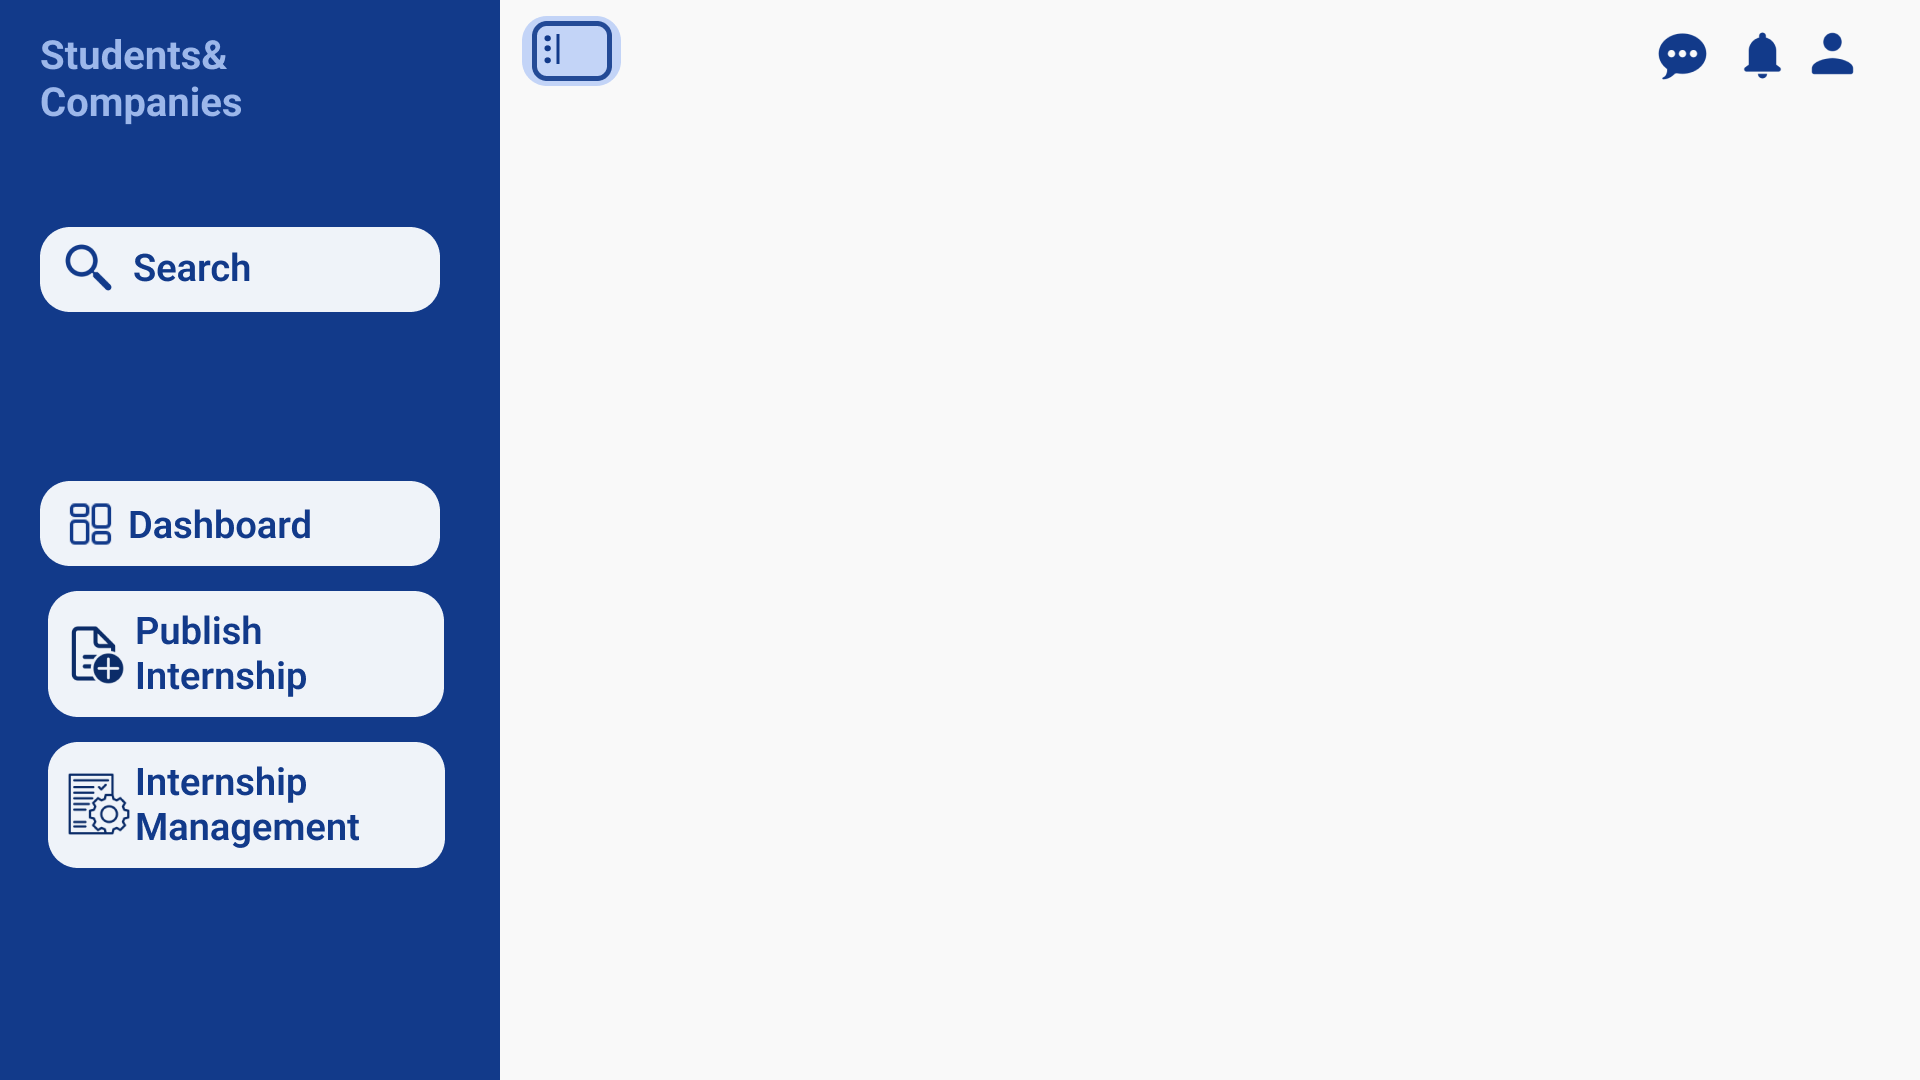
\includegraphics[width=0.8\textwidth]{Images/UI/Layout-Company.png}
    \caption{Company's Side Menu}\label{fig:Company_view}
\end{figure}
\subsubsection{Dashboard page}
Similar to the student's view, the company is directed to the Dashboard page upon logging in.
At the top of the page, the company can use the search bar as well as the search bar presented in the student's view.\\
The Dashboard provides an overview that allows companies to quickly assess the announcements they have published
and allows them to access directly to the publish internship page by clicking on the \textit{Publish new internship} button.\\
Below that, there is a section In progress internship overview that allows companies to monitor the status of the internships in progress 
and clicking on the open button will redirect the company to the feedback and complaint page for the that internship.\\
\begin{figure}[H]
    \centering
    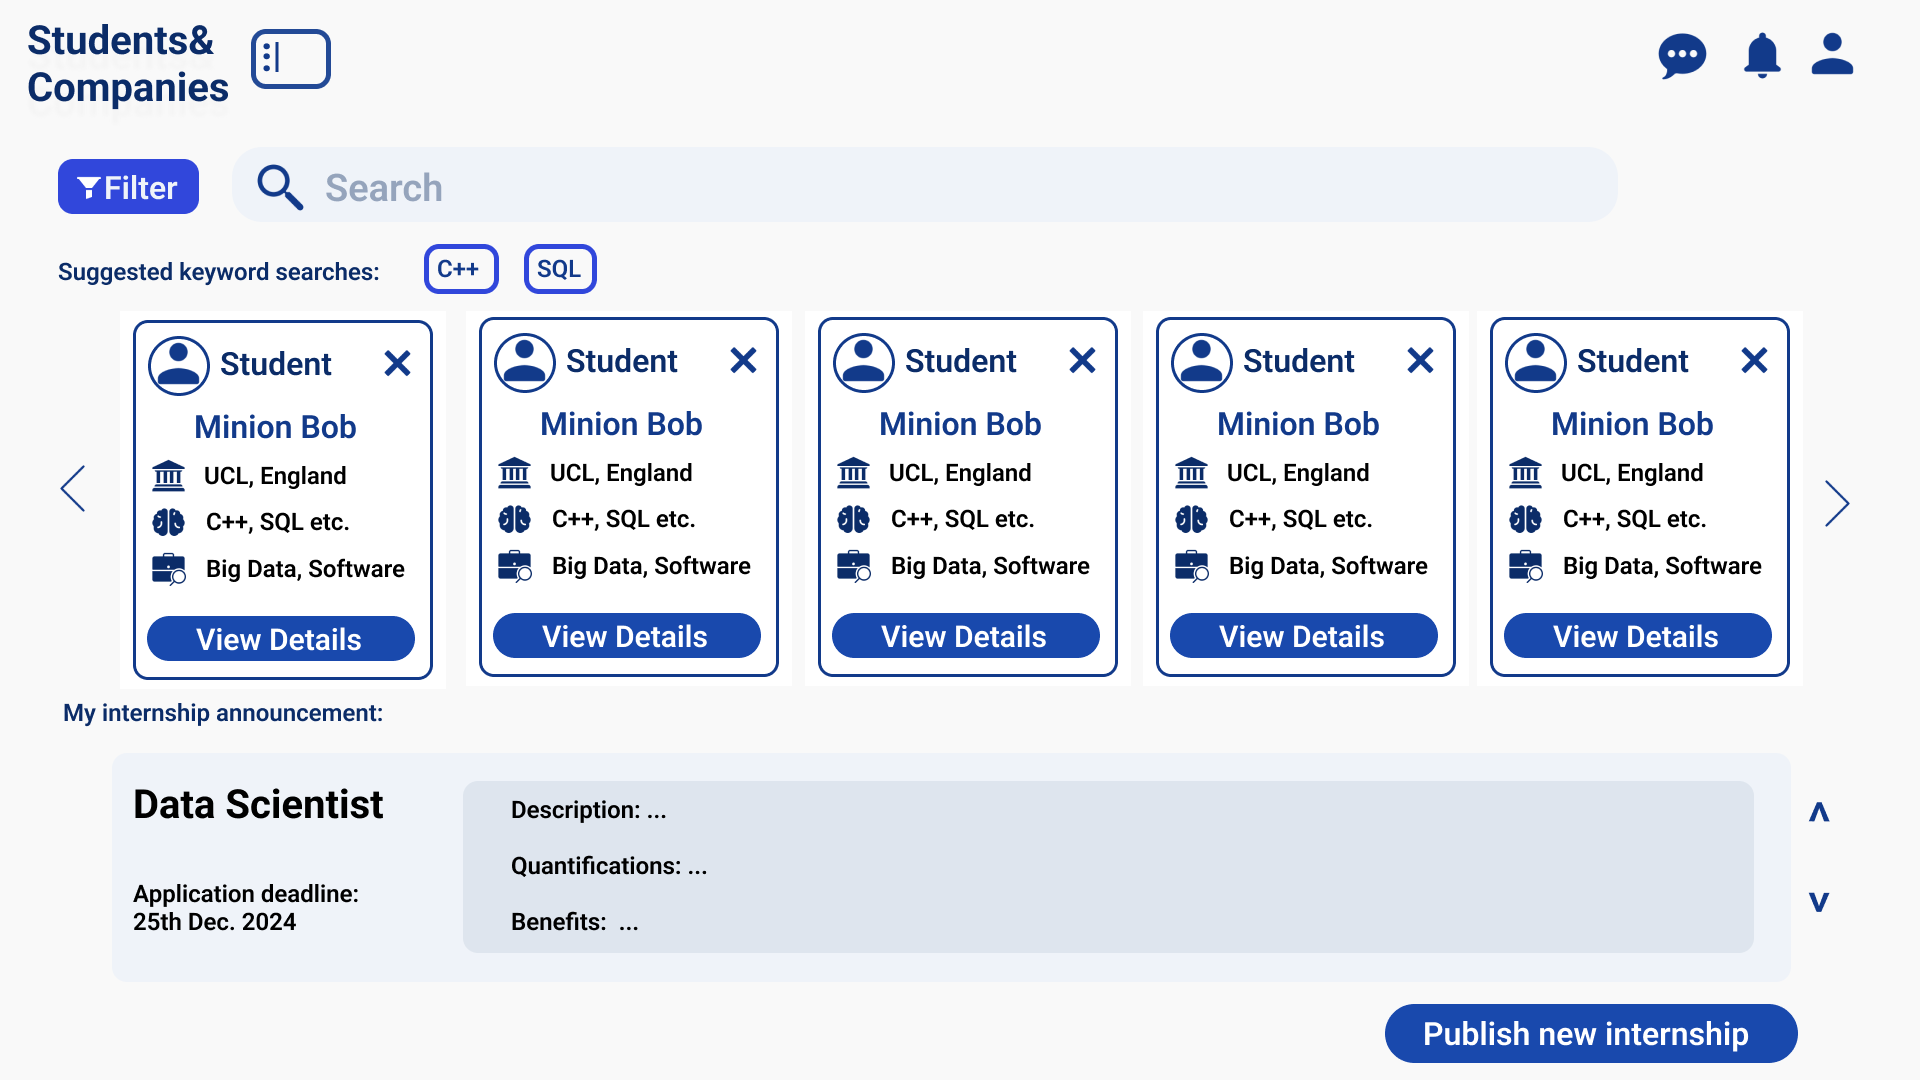
\includegraphics[width=0.8\textwidth]{Images/UI/Dashboard 1-company.png}
    \caption{Company's Dashboard 1}\label{fig:DashboardCompany1}
\end{figure}

\begin{figure}[H]
    \centering
    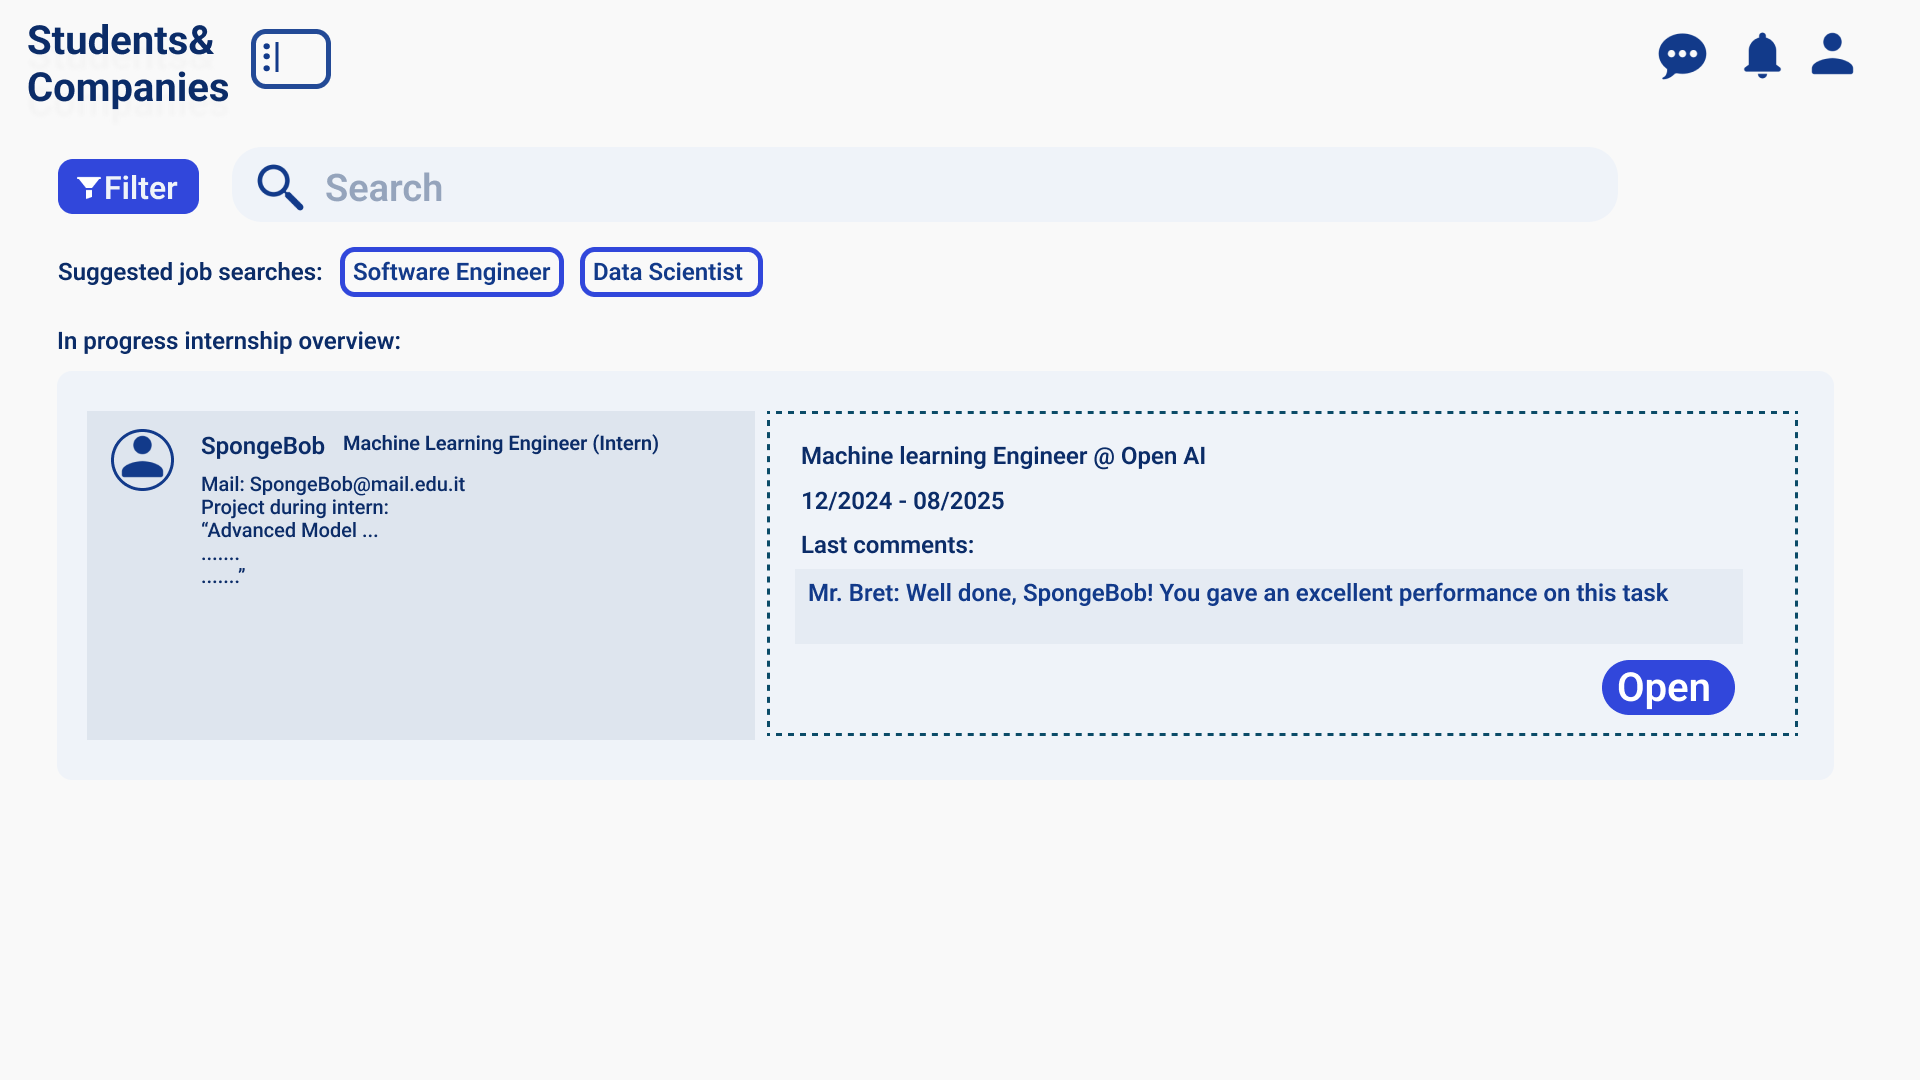
\includegraphics[width=0.8\textwidth]{Images/UI/Dashboard 2-company.png}
    \caption{Company's Dashboard 2}\label{fig:DashboardCompany2}
\end{figure}
\subsubsection{Publish Internship page}
In this page, the company can fill in the required information to publish a new internship announcement on the platform.
\begin{figure}[H]
    \centering
    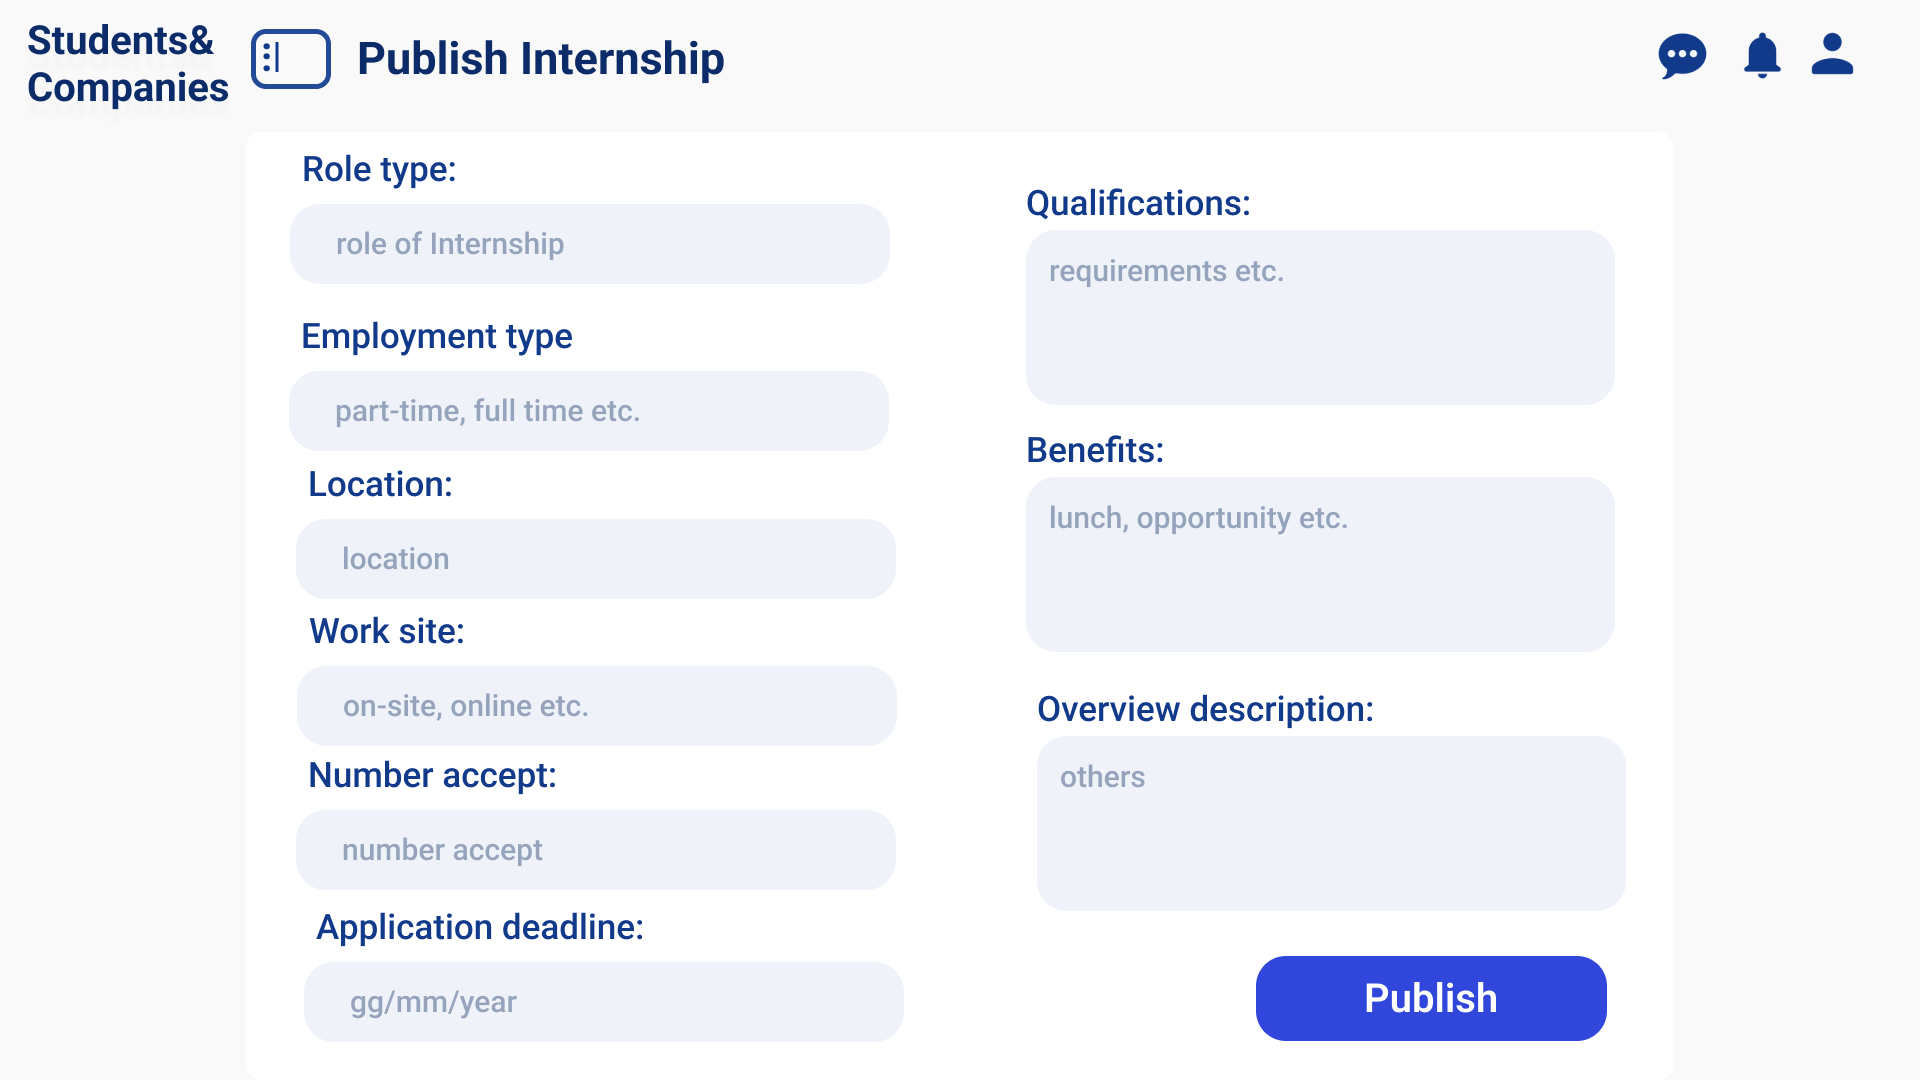
\includegraphics[width=0.8\textwidth]{Images/UI/Publish Internship -company.png}
    \caption{Publish Internship}\label{fig:Publish Internship}
\end{figure}

\subsubsection{Internship Management page}
Here in figure\ref{fig:Internship Management 1}, the company can view the list of internships they have published and take action based on the status of the internship:
\begin{itemize}
    \item[-] In publishing, means the internship announcement is still open for students to apply, the company can click on the \textit{View details} button to view the page with details of the internship announcement, figure\ref{fig:Internship details in publishing phase}.
    \item[-] In selection, means the deadline is reached and the internship enter in selection phase, the company can click on the 
    \textit{Select candidates} button to view the list of candidates who have applied for the internship and take action to select 
    the candidates to process the interview, figure\ref{fig:Select candidates}.
    \item[-] In progress, means that internship is in progress, the company can click on the \textit{Add comments} button to access the feedback and complaints page for the internship, figure\ref{fig:Feedback and Complaint}.
    \item[-] Completed, means that internship is finished, the company can click on the \textit{View details} button to view the announcement details and feedback and complaints recorded by the company and the student during the internship.
\end{itemize}

\begin{figure}[H]
    \centering
    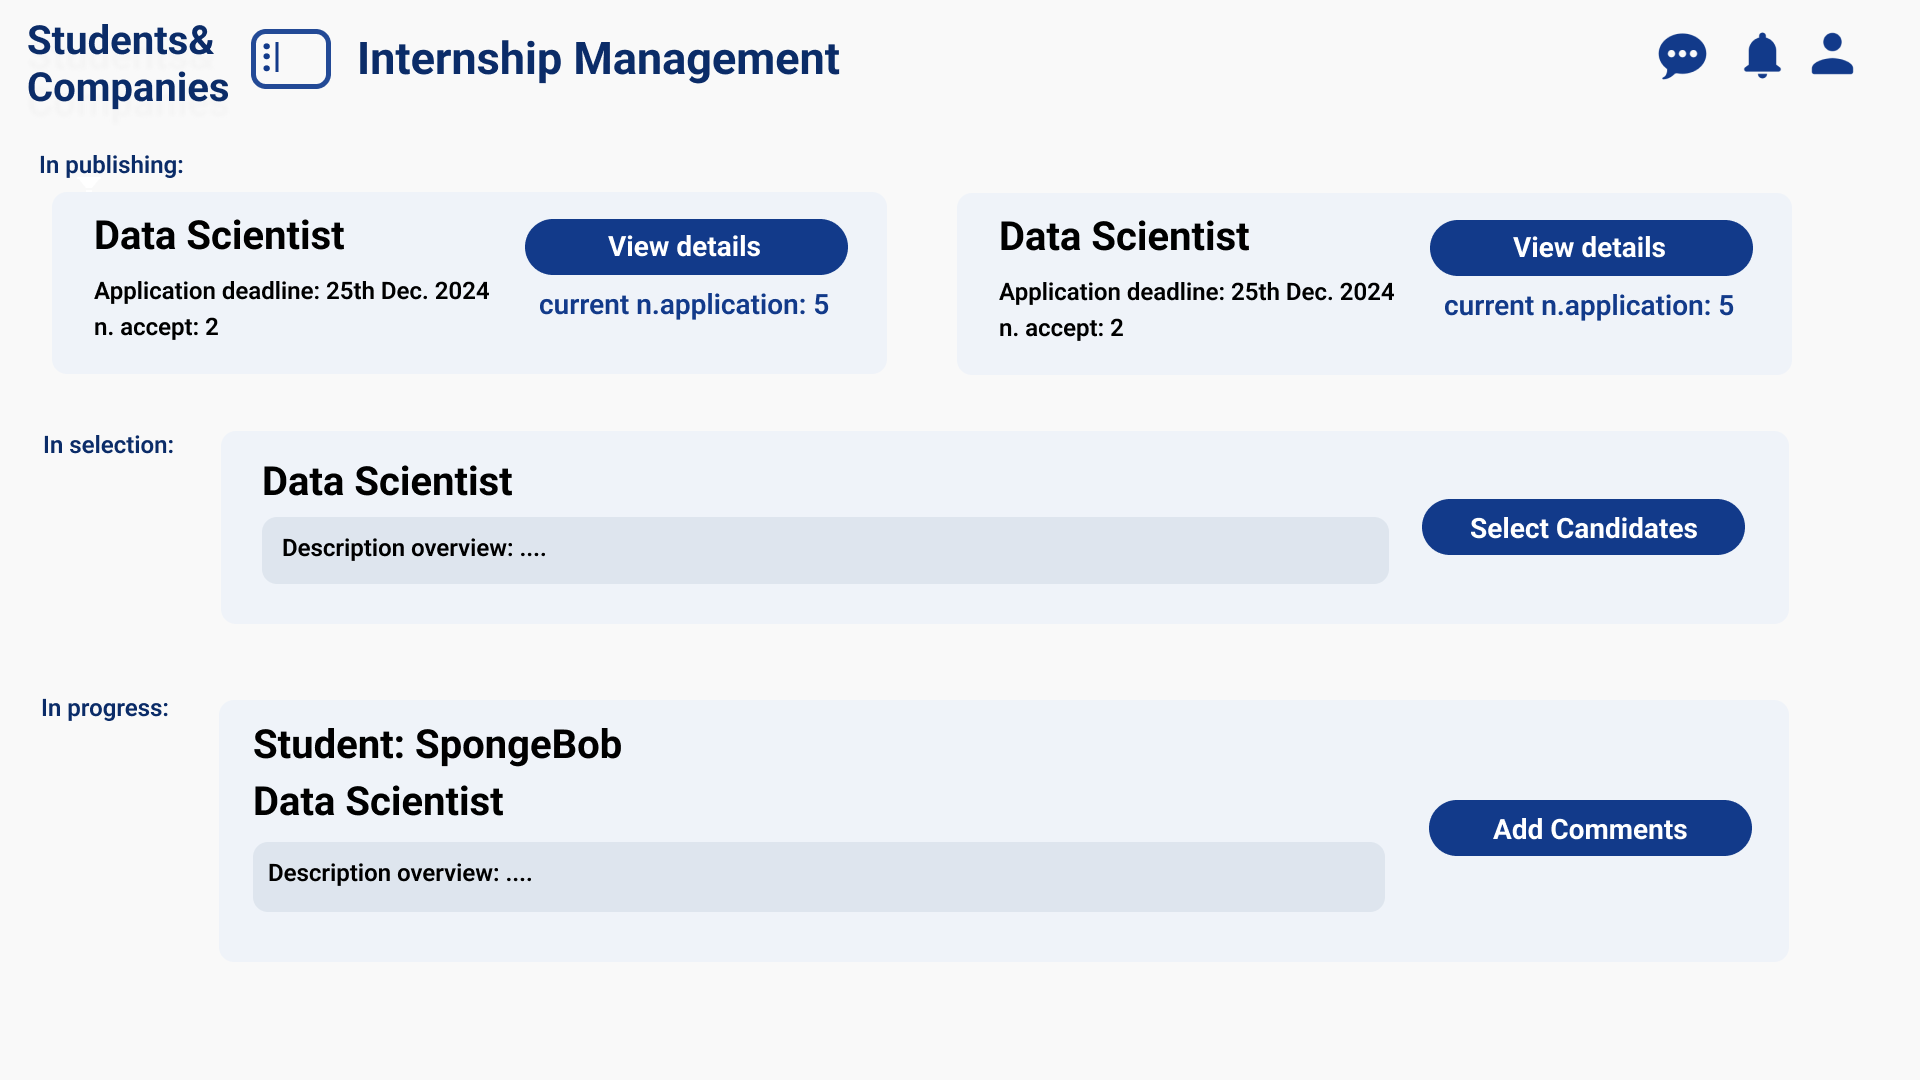
\includegraphics[width=0.8\textwidth]{Images/UI/Internship Management-company.png}
    \caption{Internship Management 1}\label{fig:Internship Management 1}
\end{figure}

\begin{figure}[H]
    \centering
    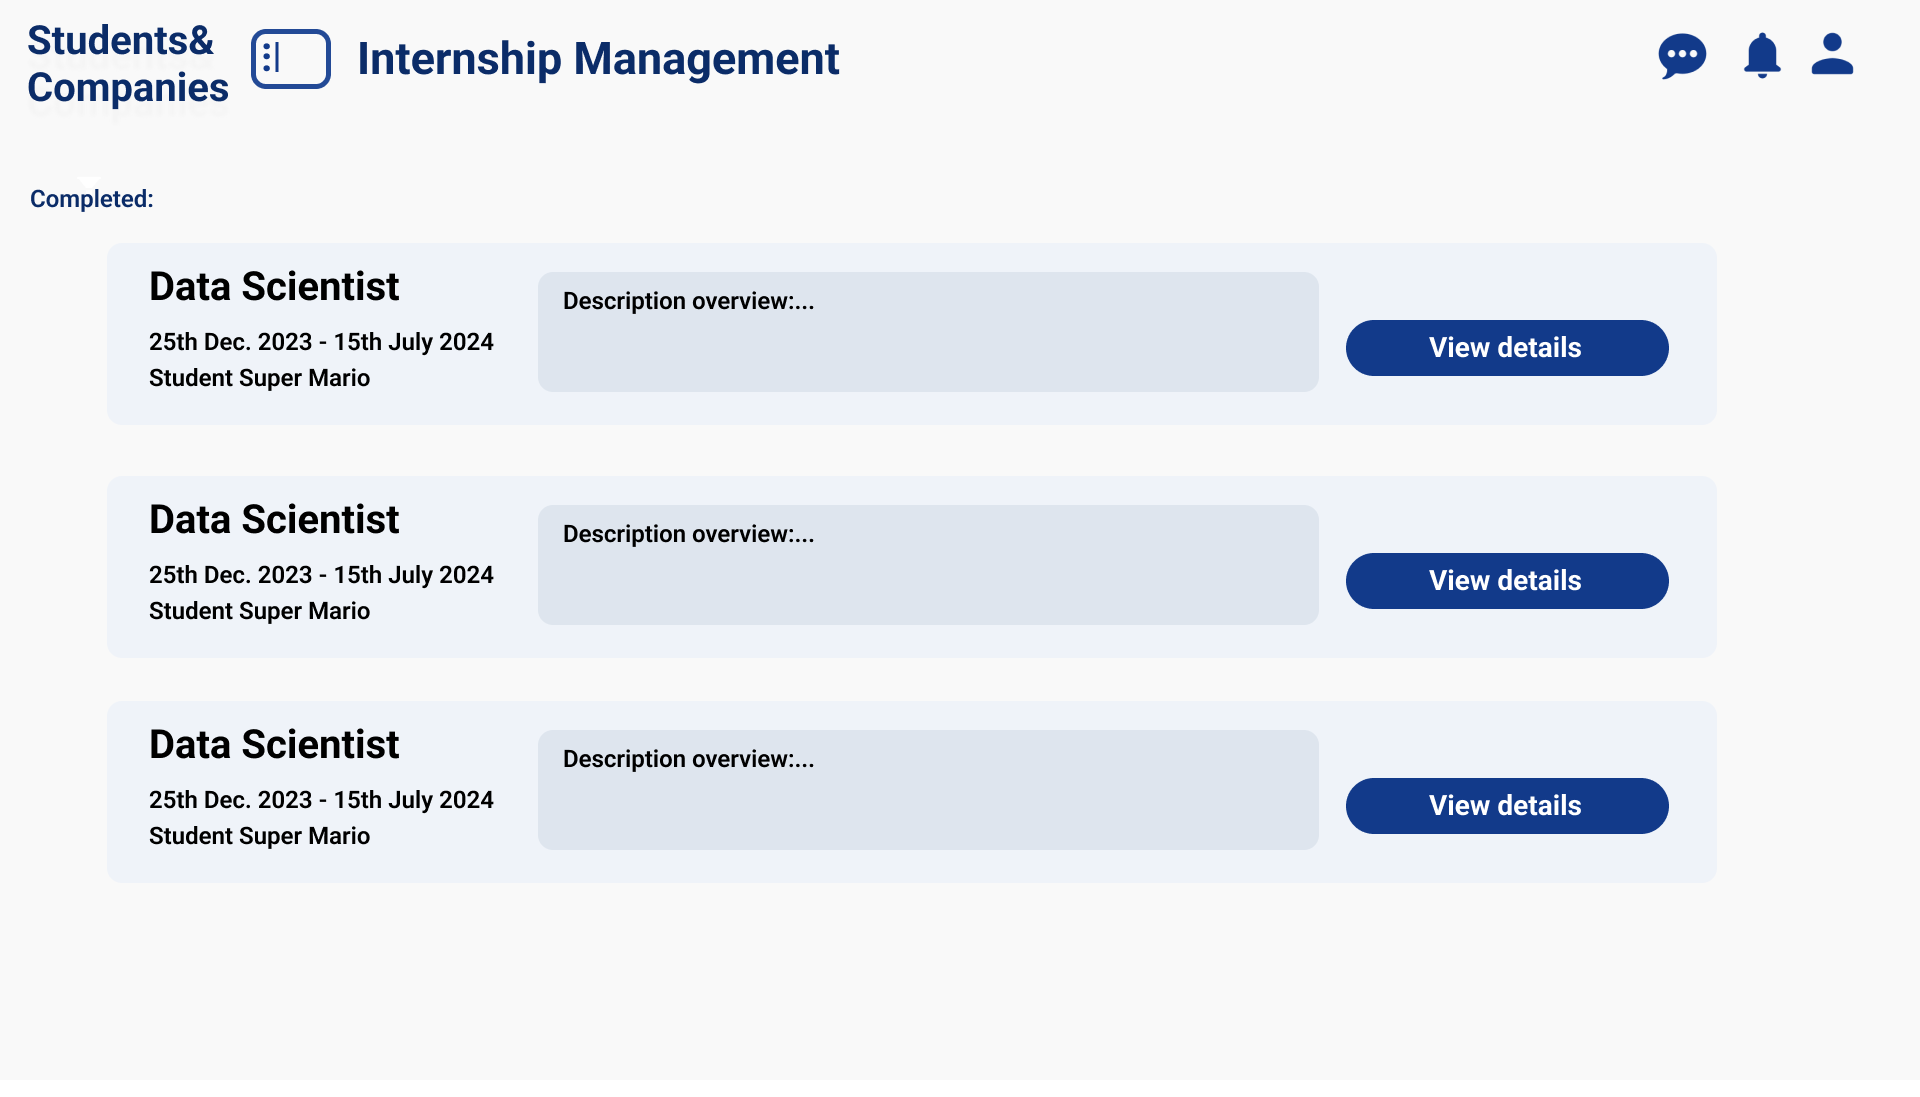
\includegraphics[width=0.8\textwidth]{Images/UI/Internship Management2-company.png}
    \caption{Internship Management 2}\label{fig:Internship Management 2}
\end{figure}

\subsubsection{Internship details page}
The internship details page in selection phase, the company can view the list of candidates who 
have applied for the internship and select the candidates to process the interview by clicking on the button \textit{process interview}.
\begin{figure}[H]
    \centering
    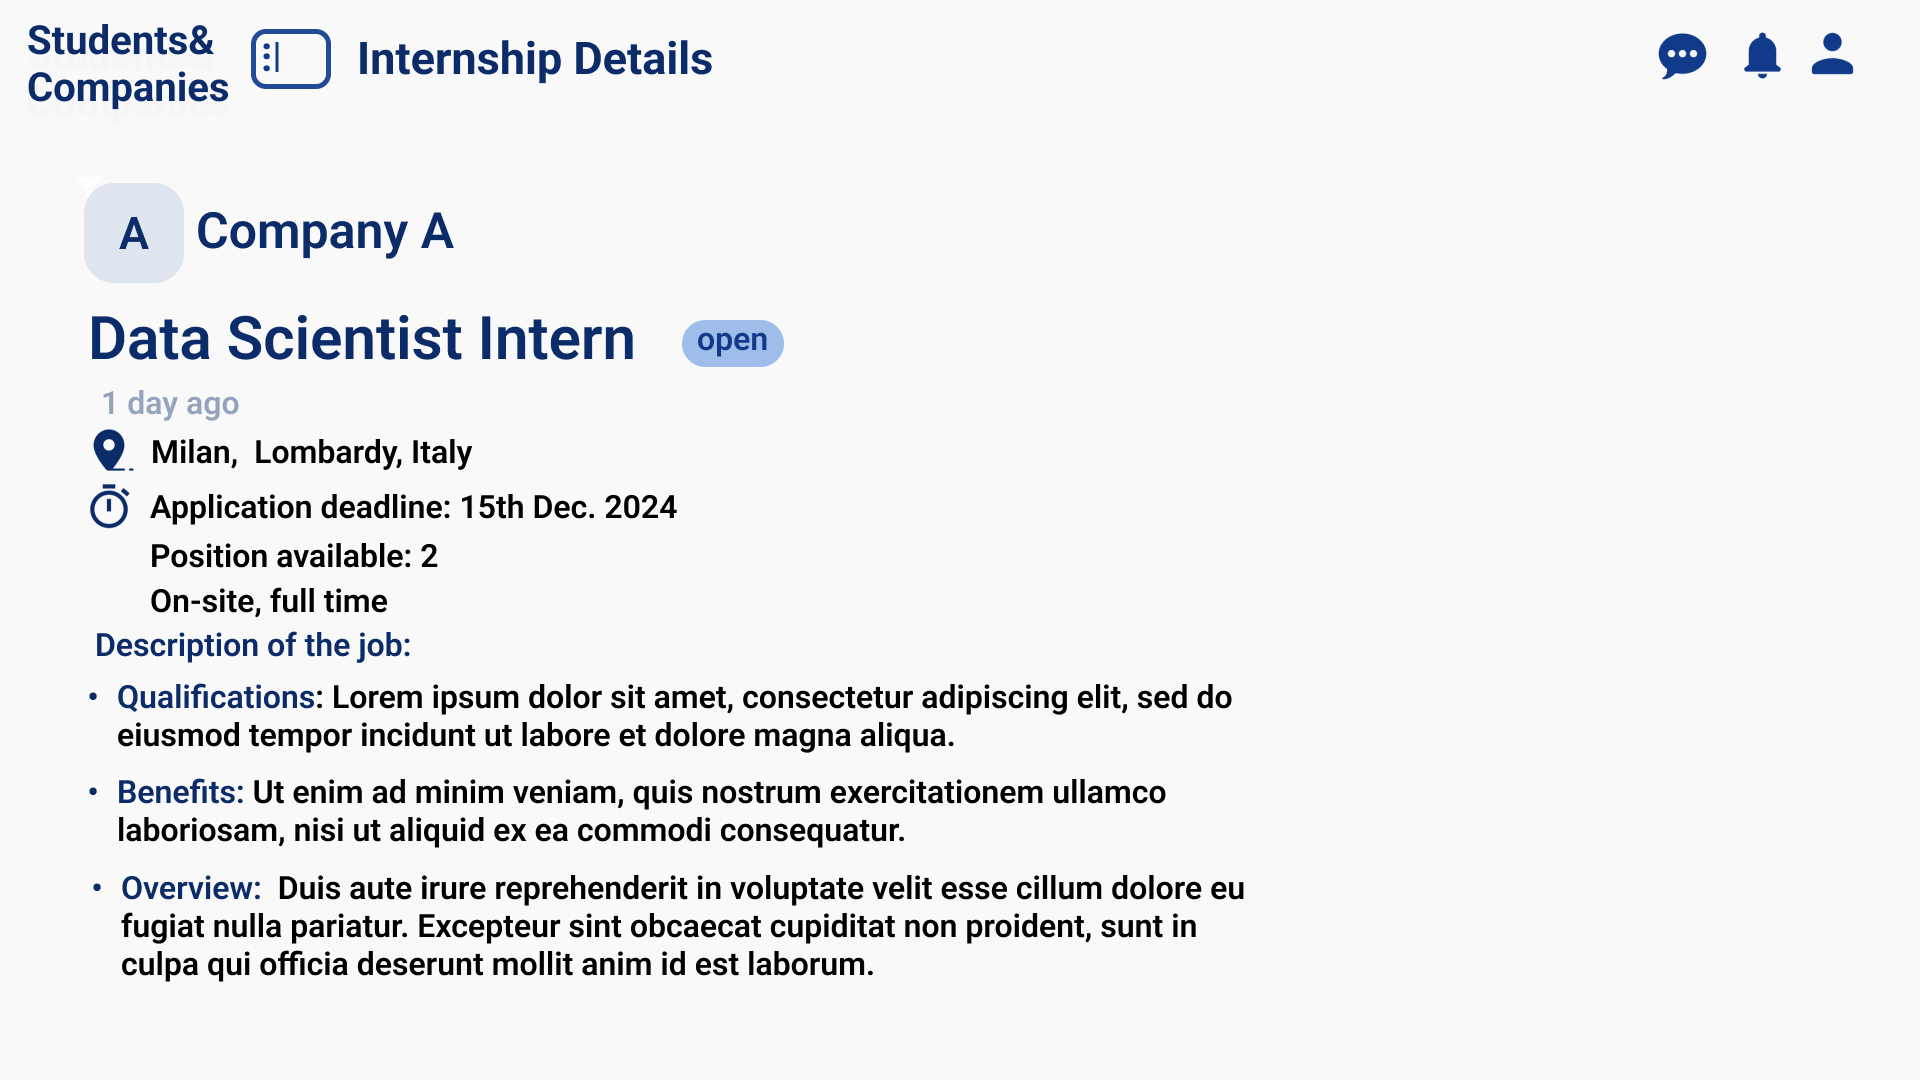
\includegraphics[width=0.8\textwidth]{Images/UI/Internship details-company view.png}
    \caption{Internship details in publishing phase}\label{fig:Internship details in publishing phase}
\end{figure}
\begin{figure}[H]
    \centering
    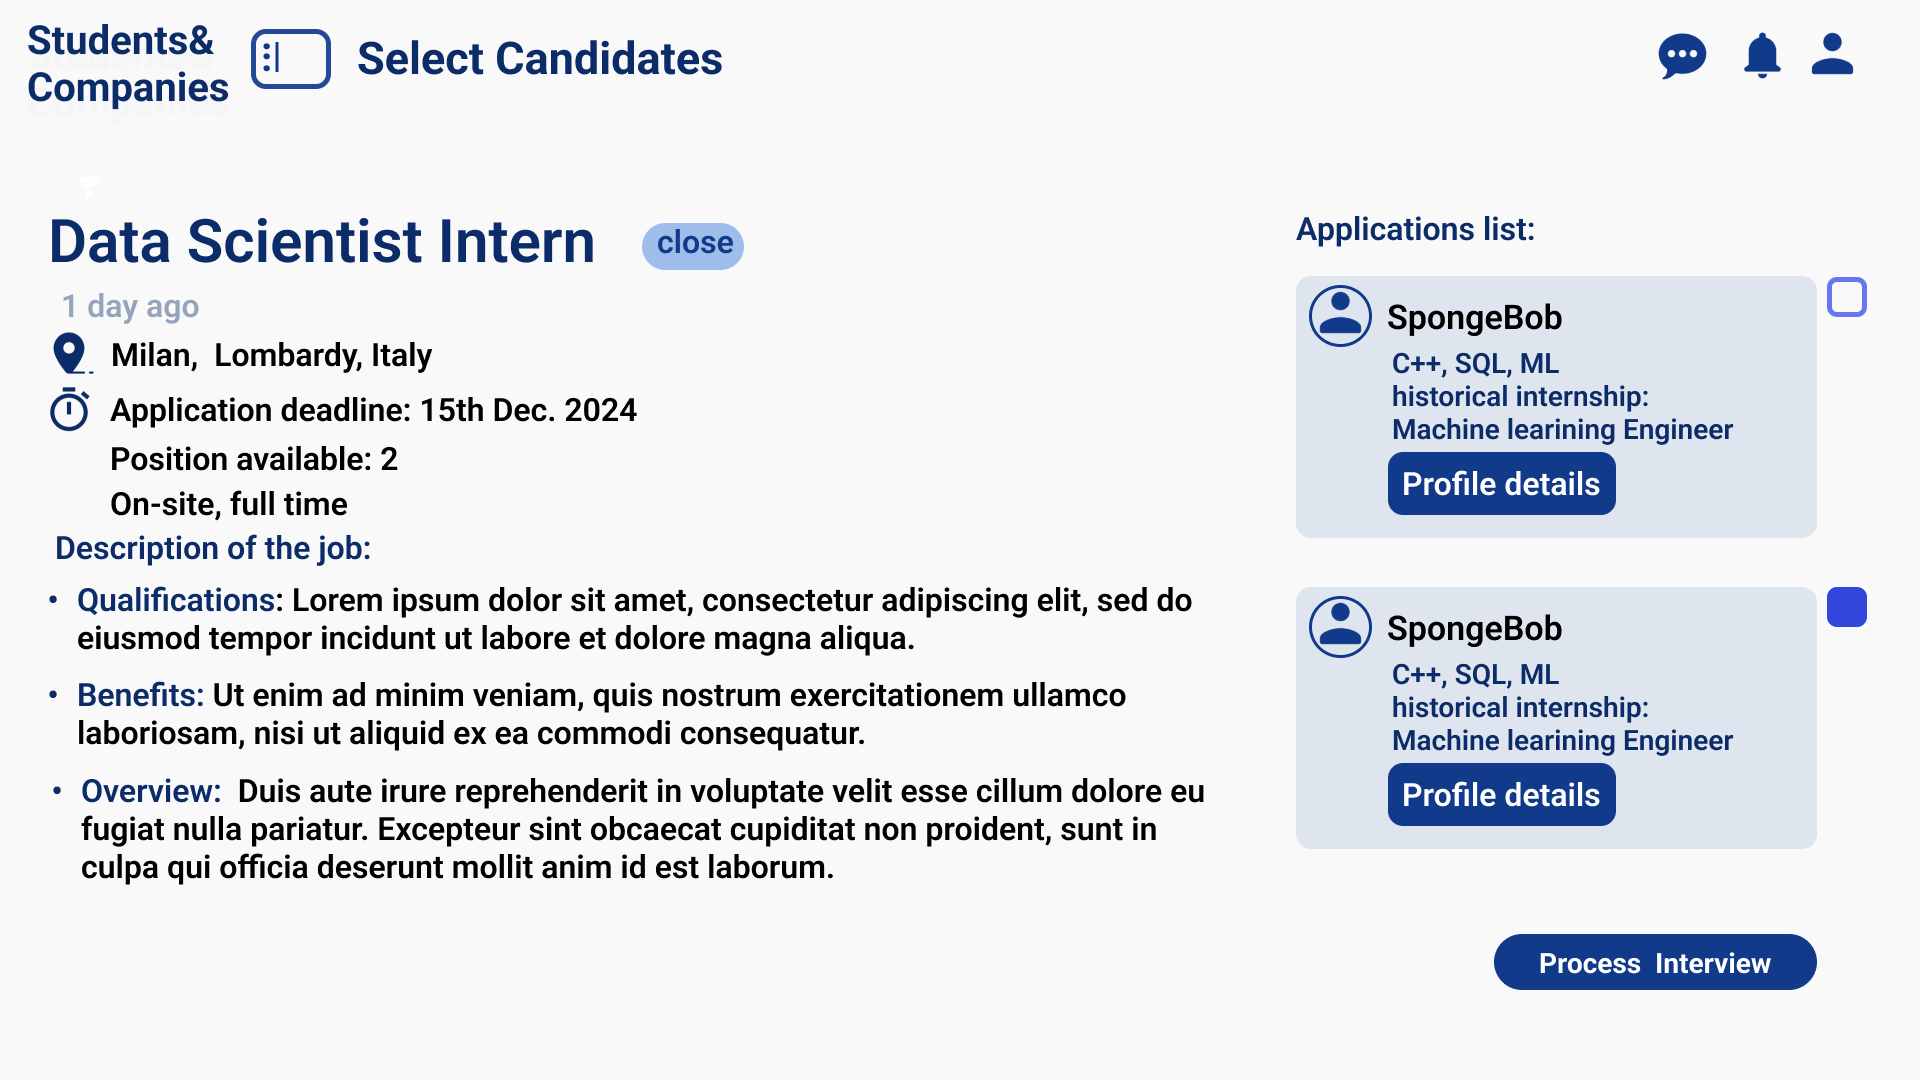
\includegraphics[width=0.8\textwidth]{Images/UI/Select candidates.png}
    \caption{Select candidates}\label{fig:Select candidates}
\end{figure}

\subsubsection{Interview set up page}
In this page, the company can write the invitation letter with the necessary information for the interview and prepare
the questionnaire to ask the candidate to fill in before the interview. Clicking on the \textit{Submit} button will send 
the invitation letter and the questionnaire to the student selected for the interview.
\begin{figure}[H]
    \centering
    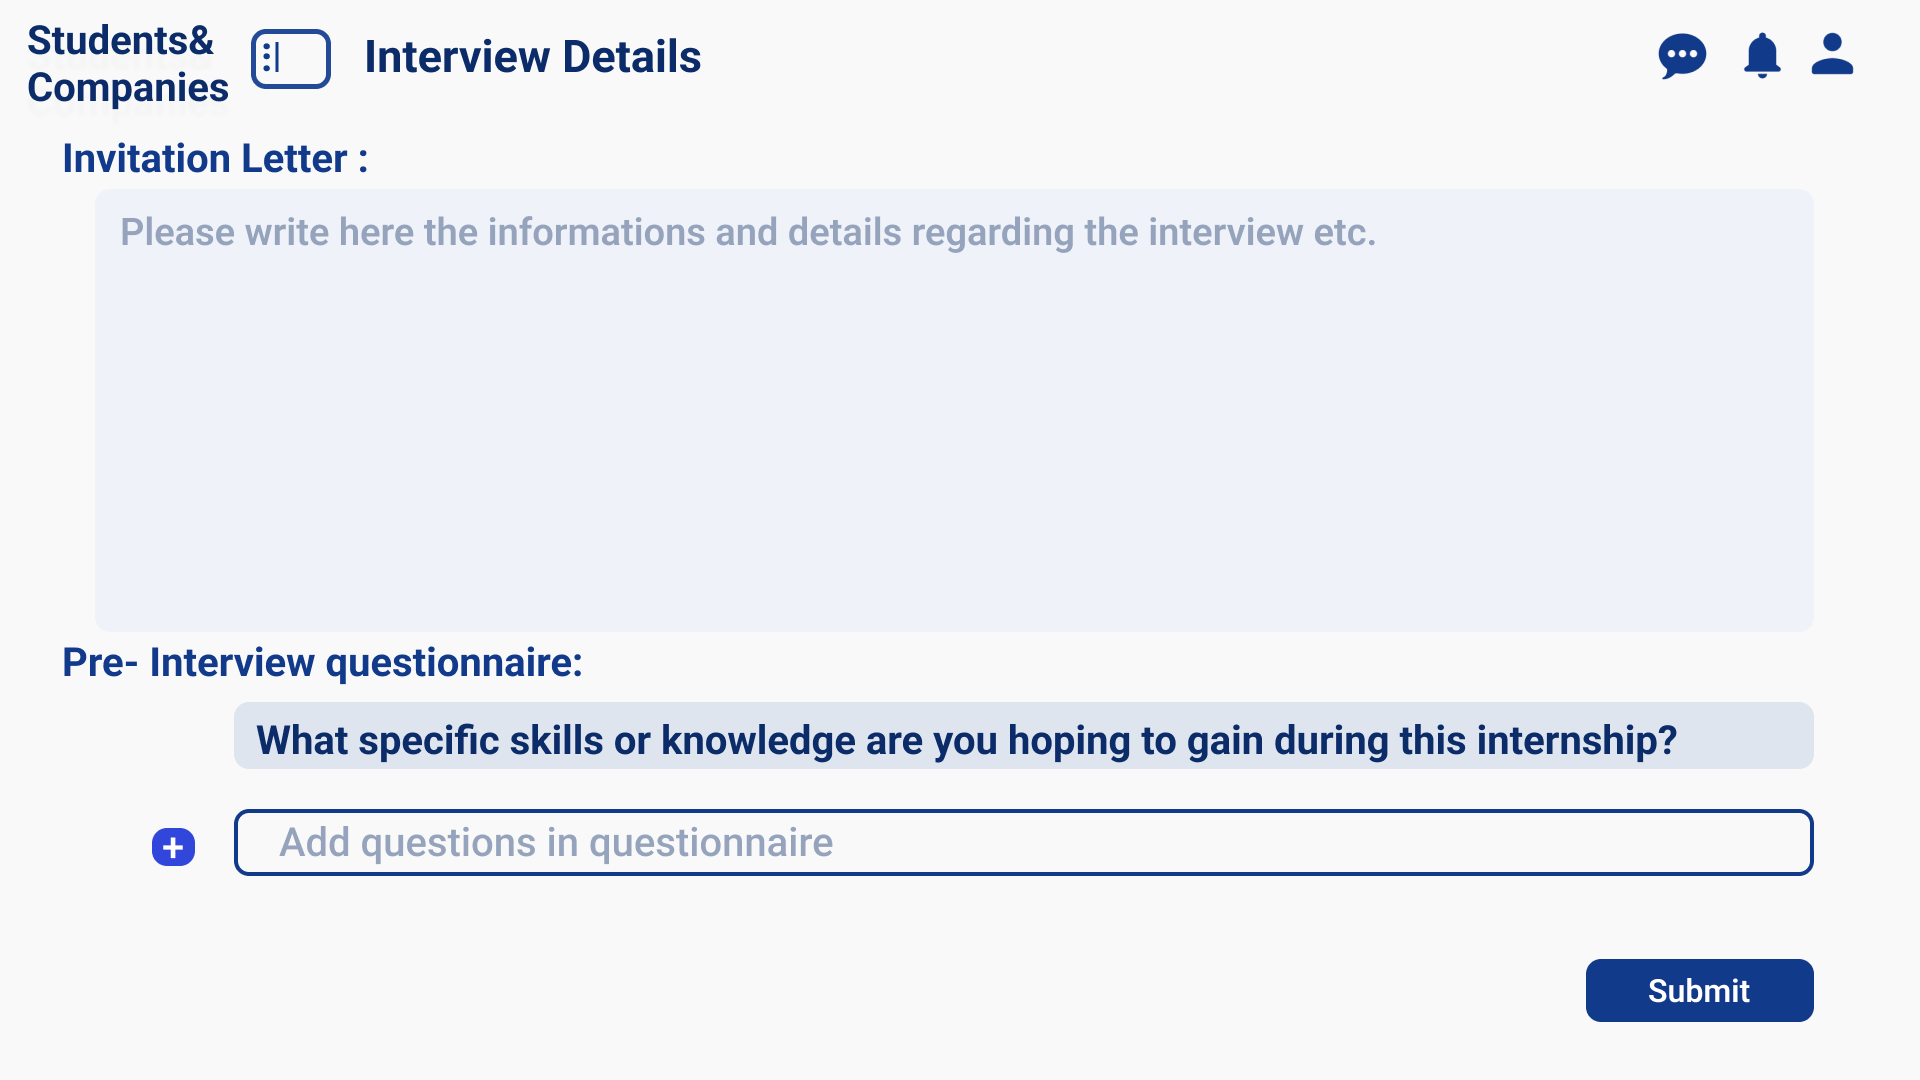
\includegraphics[width=0.8\textwidth]{Images/UI/Set Interview-Company.png}
    \caption{Set up interview}\label{fig:Set up interview}
\end{figure}

\subsubsection{Company profile page}
Figure\ref{fig:Company's profile from other's view} shows a company's profile from the 
prospective of other's user once looking for its profile.
Including the company brief description, contact email, specific fields of the company that 
the company is focusing on and the list of internships the company has published.
\begin{figure}[H]
    \centering
    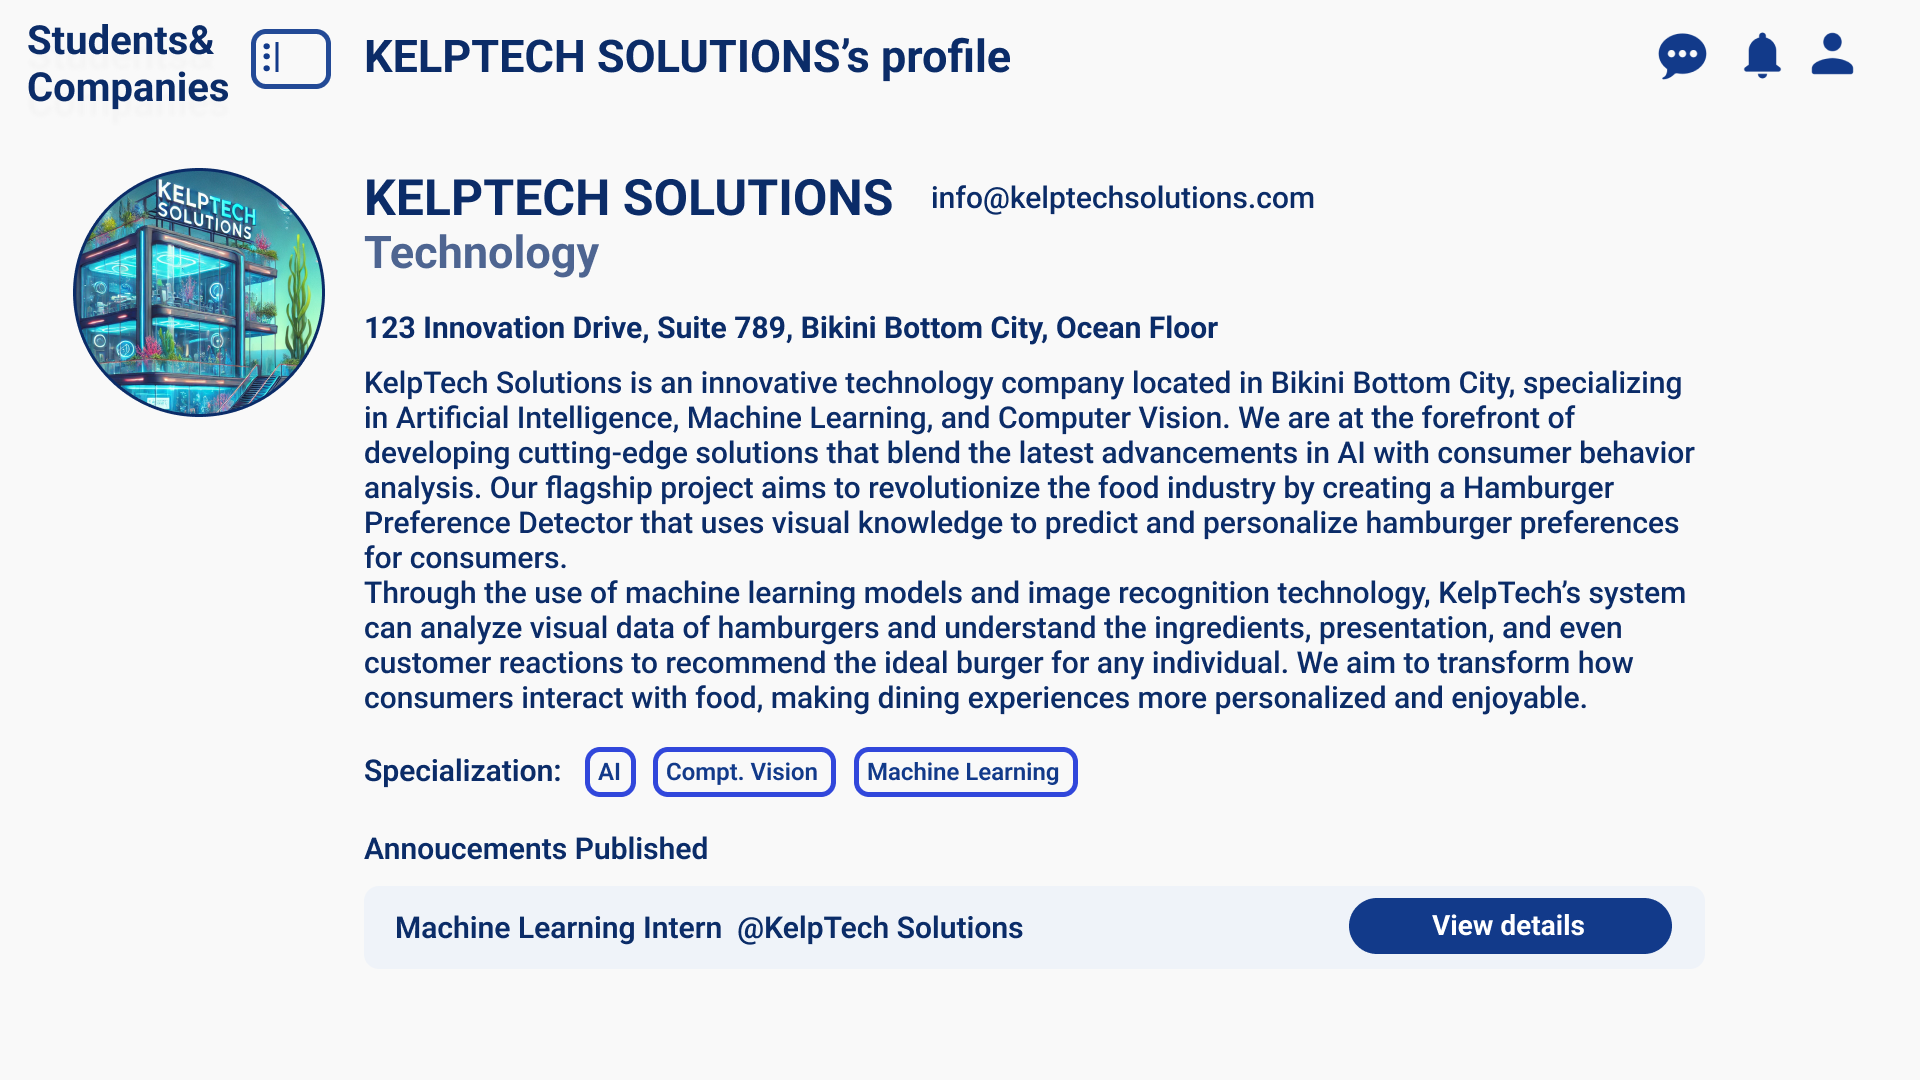
\includegraphics[width=0.8\textwidth]{Images/UI/Company profile.png}
    \caption{Company's profile from other's view}\label{fig:Company's profile from other's view}
\end{figure}

\newpage
\subsection{Student and Company's view}
\subsubsection{FeedBack and Compalint page}
Figure\ref{fig:Feedback and Complaint} shows the page where the involved parties can leave feedback and complaints about the internship.
There are two blocks, one shows the feedback and complaints history and one is the box where the user can 
write the feedback or complaint.
\begin{figure}[H]
    \centering
    \includegraphics[width=0.8\textwidth]{Images/UI/FeedBack&Complaint- Student & Company.png}
    \caption{Feedback and Complaint}\label{fig:Feedback and Complaint}
\end{figure}

\newpage
\subsection{University's view}
For the university, the GUI is more simple than the student and company's view, because the university has only 
the role of monitoring the activities of its students.
As other users, the university can use the side menu to navigate to the desired page:
\textit{Search},\textit{Dashboard}.
\begin{figure}[H]
    \centering
    \includegraphics[width=0.8\textwidth]{Images/UI/Layout-University.png}
    \caption{University's Side Menu}\label{fig:University_view}
\end{figure}
\subsubsection{Dashboard page}
The university is directed to the Dashboard page upon logging in. The search bar, the Student list and a 
specific student's activities overview will be displayed in this page. To change the student, click on 
the box of certain student in the Student list, the student's activities overview will be updated and showed
respectively. If the university wants to view the Student's profile, click on the \textit{Profile details} button.
\begin{figure}[H]
    \centering
    \includegraphics[width=0.8\textwidth]{Images/UI/Dashboard 1-university.png}
    \caption{University's Dashboard 1}\label{fig:DashboardUniversity1}
\end{figure}

\subsubsection{FeedBack and Compalint page}
This page will be displayed when the university click on the \textit{View details} button of one of the student's activities.
The university can view the feedback and complaints history written by the student and the company during the internship and 
at the end of the internship.

\begin{figure}[H]
    \centering
    \includegraphics[width=0.8\textwidth]{Images/UI/FeedBack&Complaint- University view.png}
    \caption{Feedback and Complaint}\label{fig:Feedback and Complaint University}
\end{figure}

\clearpage
\chapter{Requirements Traceability}\label{sect:requirements tracebility}
\subsubsection{Authorization Manager}
\paragraph{Registration Manager}
\begin{itemize}
    \item \textbf{R1}: S\&C allows unregistered Users to sign up
\end{itemize}

\paragraph{Login Manager}
\begin{itemize}
    \item \textbf{R2}: S\&C allows registered Users to login
\end{itemize}


\subsubsection{User Manager}
\paragraph{Profile Modification Manager}
\begin{itemize}
    \item \textbf{R3}: S\&C allows STs to upload their CV in their profile section
    \item \textbf{R36}: S\&C allows Users to modify their own profile data
\end{itemize}

\paragraph{View Profile Manager}
\begin{itemize}
    \item \textbf{R34}: S\&C allows UNIs to access the list of all the enrolled STs that are registered on the platform
    \item \textbf{R35}: S\&C allows Users to visualize the own and other users' profiles
\end{itemize}


\subsubsection{Search Manager}
\begin{itemize}
    \item \textbf{R4}: S\&C allows STs to search for internships
\end{itemize}


\subsubsection{Notification Manager}
\begin{itemize}
    \item \textbf{R8}: S\&C should notify STs when they are selected by the CO for the interview process
    \item \textbf{R9}: S\&C should notify STs when a CO is interested in their profile
    \item \textbf{R10}: S\&C should notify STs when he is successfully selected for a position
    \item \textbf{R11}: S\&C should notify STs when a CO rejects their application
    \item \textbf{R12}: S\&C should notify UNIs when their students start an internship
    \item \textbf{R13}: S\&C should notify STs when an internship available matches their interest
    \item \textbf{R14}: S\&C should notify COs when the deadline for a published internship has expired
    \item \textbf{R15}: S\&C should notify COs when the candidate accepts the position
    \item \textbf{R16}: S\&C should notify COs when the candidate refuses the position
    \item \textbf{R17}: S\&C should notify COs and STs when a new chat message is available
    \item \textbf{R18}: S\&C should notify COs when a ST with a CV that corresponds to their needs is available
    \item \textbf{R37}: S\&C  should notify UNIs when their students register on the platform
\end{itemize}


\subsubsection{Recommendation Module}
\begin{itemize}
    \item \textbf{R19}: S\&C should be able to analyze the User's data to provide the recommendations to both STs and COs
\end{itemize}


\subsubsection{Internship Manager}
\paragraph{Creation Manager}
\begin{itemize}
    \item \textbf{R5}: S\&C allows COs to create internships by compiling all the information
    \item \textbf{R6}: S\&C allows COs to set a deadline for submitting the application to an internship
    \item \textbf{R7}: S\&C  allows COs to publish internships
\end{itemize}

\paragraph{View Internship Information Manager}
\begin{itemize}
    \item \textbf{R21}: S\&C allows STs to visualize information about a published internship
    \item \textbf{R33}: S\&C allows UNIs to check the status of the internship records of their students
\end{itemize}

\paragraph{Selection Manager}
\begin{itemize}
    \item \textbf{R23}: S\&C allows COs to record STs selection outcomes
\end{itemize}

\paragraph{Feedback Manager}
\begin{itemize}
    \item \textbf{R30}: S\&C allows STs and COs to write feedback and complaints relating to the internship experience
    \item \textbf{R31}: S\&C allows Users to view feedback and complaints relating to the internship experience
\end{itemize}

\paragraph{Chat Manager}
\begin{itemize}
    \item \textbf{R32}: S\&C allows STs and COs to exchange information using the chat, only if the ST is participating or has participated 
                        in an internship offered by the company
\end{itemize}


\subsubsection{Application Manager}
\paragraph{Submission Manager}
\begin{itemize}
    \item \textbf{R20}: S\&C allows STs to submit their application for an internship
    \item \textbf{R29}: S\&C allows STs to accept or reject the offer after receiving the interview results
\end{itemize}

\paragraph{View Application Information Manager}
\begin{itemize}
    \item \textbf{R22}: S\&C allows COs to view the list of all applications that were submitted for a specific internship
    \item \textbf{R28}: S\&C allows STs to check the status of their applications
\end{itemize}

\paragraph{Interview Manager}
\begin{itemize}
    \item \textbf{R24}: S\&C allows COs to create forms to submit to candidates for the interview process
    \item \textbf{R27}: S\&C allows COs to record the results of the interview
\end{itemize}

\paragraph{Questionnaire Manager}
\begin{itemize}
    \item \textbf{R25}: S\&C allows candidates to respond to the received forms
    \item \textbf{R26}: S\&C allows COs to visualize the responses of the candidates who have replied to the forms 
\end{itemize}


\clearpage
\chapter{Implementation, Integration and Test Plan}\label{sect:implementation}
\renewcommand{\thesection}{\Alph{section}}
To implement the system more effectively and efficiently, it is crucial to stabilize the development process. This provides a clear 
understanding of the tasks to be completed, their order of execution, and a reliable reference framework for teams working collaboratively 
on the same project. Therefore a proper planning for implementation and testing is essential. In following sections will be presented the
strategy in this phase of the project: the implementation plan, the integration plan, and the testing plan.

As the platform consists of several components and features, each with varying levels of complexity and dependencies on other components, 
the Bottom-Up is the suitable approach to optimize the development process. This approach allows team members to work independently on 
different parts of the system simultaneously. The process begins with the leaves of the "use" hierarchy and progresses upward toward the root.
This typically requires the creation of multiple drivers, one for each module. By following this approach, several subsystems will be developed 
and with the continuous integration of these subsystems, the final system will be created.

\section{Implementation Plan}\label{sec:implementation-plan}
The priority of components to be implemented is determined by their functionality and the dependencies between them. Since the system is divided 
into a set of components, as described in Section \ref{sect:architectural design}, the following list outlines the importance of each component
at the development stage, allowing for a smooth and efficient build process.
\begin{table}[H]
    \centering
    \begin{tabular}{|c|c|}
        \hline
        \textbf{Component} & \textbf{Priority} \\
        \hline
        Model Module & Very High \\
        \hline
        Notification Manager & Low \\
        \hline
        Authentication Manager & Medium \\
        \hline
        User Manager & High \\
        \hline
        Internship Manager & High \\
        \hline
        Application Manager & High \\
        \hline
        Recommendation Module & Medium \\
        \hline
        Search Module & Low \\
        \hline
    \end{tabular}
    \caption{Implementation Plan}\label{tab:implementation-plan}
\end{table}

 The Model Module serves as the foundation for all other components, meaning it is responsible for managing the platform's data. It facilitates
 communication between other components and the DBMS, providing an interface for accessing the data. Therefore, it should be implemented in 
 the first stage. Next, there is the Notification Manager supports communication between other components, such as the Authentication Manager, 
 Internship Manager, and Application Manager. After that, the Authentication Manager should be implemented, as it is an essential first step 
 for accessing the platform and controlling access to other components. Then following the dependency tree, the User Manager should then be 
 implemented which is responsible for managing user data and providing an interface for user-related operations. Once the basic components are
 are implemented, the core functions of the platform—the Internship Manager and Application Manager—can be developed. Afterward, the Search 
 Module and Recommendation Module can be implemented at the last stage, as they are secondary functions that are closely connected to the 
 platform's core functionalities.

\section{Integration Plan}\label{sec:integration-plan}
In this section will specify the order in which the components will be integrated and the components of each manager described in the
previous paragraph. The integration process will be divided into two main phases: the first phase will focus on integrating the components
of each manager, while the second phase will focus on integrating the managers themselves. Also during the integration process, the
unit testing and the integration testing will be performed to ensure that the components are working correctly by adding the functionalities
to the system.
\begin{enumerate}
    \item \textbf{Model Module:} The connection between the Model Module and the DBMS will be established first, as it is responsible for 
    managing the platform's data and providing an interface for other components to access the data.
    \begin{figure}[H]
        \centering
        \includegraphics[width=0.16\textwidth]{Images/BottomUp/Model.png}
    \end{figure}
    \item \textbf{Notification Manager:} The Notification Manager will be integrated next with the Model Module, at this stage, the connection
    between the Notification Manager and the Model Module will be established and tested.
    \begin{figure}[H]
        \centering
        \includegraphics[width=0.2\textwidth]{Images/BottomUp/Notification.png}
    \end{figure}
    \item \textbf{Authentication Manager:} The Authentication Manager, including the Registration and Login Manager, will be integrated next, 
    as these are the basic functionalities for accessing the platform. After interaction with the Model Module and the Notification Manager, 
    their functionalities will be tested to ensure that reading and writing operations in the database work correctly and that notifications 
    are sent properly during the registration and login processes. Additionally, the communication with the external email service will be verified.
    \begin{figure}[H]
        \centering
        \includegraphics[width=0.4\textwidth]{Images/BottomUp/Auth.png}
    \end{figure} 
    \item \textbf{User Manager:} As the last basic component, the View Profile Manager and Profile Modification Manager will be integrated. 
    Since they depend only on components that have already been integrated, unit testing and integration testing can be conducted to ensure that 
    all basic functionalities work correctly before moving to the integration of the core functionalities.
    \begin{figure}[H]
        \centering
        \includegraphics[width=0.7\textwidth]{Images/BottomUp/Profile.png}
    \end{figure}
    \item \textbf{Internship Manager:} The Internship Manager is the first core functionality to be integrated, as it is responsible for managing 
    internship data and providing an interface for internship-related operations. The order of integration of its components is as follows: 
    Creation Manager, View Internship Information Manager, Selection Manager, Chat Manager, and Feedback Manager, reflecting the order of processing 
    internship evolution. Unit testing is crucial at this stage, and extreme cases should be evaluated. Mock data will be used to simulate real 
    internship events. Integration testing of all components integrated so far will also be conducted to ensure that everything works without 
    conflicts or crashes.
    \begin{figure}[H]
        \centering
        \includegraphics[width=1\textwidth]{Images/BottomUp/Intern.png}
    \end{figure}
    \item \textbf{Application Manager:} Next, the Application Manager, which manages applications and controls the selection process, will be integrated. 
    The order of integration of its components is as follows: Submissions Manager, View Application Information Manager, Interview Manager, and 
    Questionnaire Manager. It must collaborate seamlessly with the Internship Manager and the User Manager. Integration testing is critical during 
    this phase since the platform's main functionalities are involved.
    \begin{figure}[H]
        \centering
        \includegraphics[width=1\textwidth]{Images/BottomUp/Application.png}
    \end{figure}
    \item \textbf{Recommendation Module:} After integrating and testing the core and basic functionalities, the Recommendation Module will be integrated. 
    This module depends on all previously developed components. Testing of the recommendation algorithm will be performed to verify that it provides 
    suitable recommendations based on the user's profile and internship experiences. 
    \begin{figure}[H]
        \centering
        \includegraphics[width=1\textwidth]{Images/BottomUp/Recomm.png}
    \end{figure}
    \item \textbf{Search Module:} Even though the Search Module is not closely related to all components developed so far, it will be integrated at the
     end of the integration process. This is because it is a secondary function closely connected to the platform's core functionalities. Once all other
      components have been integrated and tested, the Search Module can be integrated and tested. This approach ensures that any issues with the search 
      functionalities are not caused by other components.
      \begin{figure}[H]
        \centering
        \includegraphics[width=1\textwidth]{Images/BottomUp/Search.png}
    \end{figure}
    \item After completing the server-side integration, the client-side integration will be performed. The integration of server-side components with 
    client-side components will be processed, and testing of the interaction between server-side and client-side components will be conducted.
\end{enumerate}

\section{System Testing}\label{sec:testing-plan}
After the iterative testing process during the integration of the components, once the system is fully integrated, it needs to be tested as a whole
 using other testing techniques. In this section, the testing will focus on identifying any issues with the system's functionalities and determining 
 whether all the requirements are satisfied. During this phase, all different roles of project members will be involved in the testing process, 
 including developers, users, and black-box testers.
    \begin{itemize}
        \item \textbf{Functional Testing:} Functional testing is used to check if all functional requirements indicated in the RASD are fulfilled by 
        the software. Communication between different stakeholders and users is important to understand if the functionalities are truly as expected. 
        \item \textbf{Load Testing:} Load testing will check if the platform can handle the expected load, and if there are any bugs, such as memory 
        leaks, mismanagement of memory, or buffer overflows. It will also identify the upper limits of the components and help evaluate the optimal 
        architectural options. The system will be tested with increasing workloads until it reaches its capacity.
        \item \textbf{Performance Testing:} Performance testing aims to detect bottlenecks, inefficient algorithms, hardware or network issues, and
         to identify more efficient solutions to achieve specific goals. It should take into consideration response time, utilization, and 
         throughput of the system.
        \item \textbf{Stress testing:} Stress testing ensures high maintainability and availability. It verifies that the system recovers gracefully 
        after unexpected failures or crashes. The system should be tested by overwhelming its resources or reducing resources, for example, by 
        randomly shutting down and restarting ports on a network switch to observe the system's behavior.
        \item \textbf{User Interface Testing:} User interface testing is essential to ensure that the connection between the client and the server
        is established smoothly. It will also verify that the user interface is user-friendly and that the user can easily navigate from the user's
        perspective.
    \end{itemize}



\clearpage
\chapter{Effort Spent}\label{sect:effort}
In following table we provide the tracking of the effort spent by each group member in the development of this document.
\begin{table}[H]
    \centering
    \begin{tabular}{|c|c|c|}
    \hline
    \rowcolor{bluepoli!40}
    \textbf{Section} & \textbf{Jie Chen} & \textbf{Riccardo Bonfanti} \T\B \\
    \hline
     \textbf{1 – Introduction}                  & 0 hours & 1.5 hours \T\B \\
     \textbf{2 – Architectural Design}           & 0 hours & 27 hours \T\B\\
     \textbf{3 – User Interface Design}         & 0 hours & 0 hours \T\B\\
     \textbf{4 – Requirements Traceability}   & 0 hours & 2 hours  \T\B \\
     \textbf{5 – Implementation, Integration, and Test Plan}   & 0 hours & 0 hours  \T\B \\
     \hline
     \textbf{Total}                             & 0 hours & 31.5 hours \T\B \\

    \hline
    \end{tabular}
    \\[10pt]
    \caption{Effort spent for each section}\label{table:effort}
\end{table}

\clearpage
\chapter{References}\label{sect:references}
\renewcommand{\thesection}{\Alph{section}}
The names of \textit{SpongeBob SquarePants} characters referenced in this document are the intellectual property of \textit{Nickelodeon and Viacom International Inc.}
We do not claim any ownership of the copyrighted material. The use of these names is intended solely for purposes such as commentary, criticism, analysis, 
or education, and falls under the "fair use" provisions outlined in Section 107 of the Copyright Act of 1976 (Articolo 70 della Legge sul Diritto d'Autore 
italiana (Legge n. 633/1941)). This use is non-commercial and transformative in nature, with no intention of infringing upon the copyright holders' rights.

Lecture Slides of the course "Software Engineering 2", AA 2024/2025, by professor E. Di Nitto (Politecnico di Milano).

We used Draw.io for the creation of the UML diagrams - \url{https://www.draw.io/}.

We used GitHub for version control - \url{https://github.com/}.

We used Visual Studio Code IDE for development of the LaTeX document - \url{https://www.visualstudio.com/}.

We followed the Politecnico di Milano thesis template for the structure and style of the document -
\url{https://www.overleaf.com/latex/templates/classical
-format-thesis-scuola-di-ingegneria-industriale-e-dellinformazione-politecnico-di-milano/dkmvtndqkyxg}.

\end{document}